% ****************************************************************************************** % Dissertation template and document class for Princeton University
% Author  : Jeffrey Scott Dwoskin <jdwoskin@princeton.edu>
% Adapted from: http://www.math.princeton.edu/graduate/tex/puthesis.html
% ****************************************************************************************** %


%%% For print copies
%% set 'singlespace' option to set entire thesis to single space, and define "\printmode" to remove all hyperlinks for printed copies of the thesis. Delete all output files before changing this mode -- it will turn hyperref package on and off
%\documentclass[12pt,lot, lof, singlespace]{puthesis}
%\newcommand{\printmode}{}

%%% For the electronic copy, use doublespacing, define "\proquestmode" to use outlined links, instead of colored links. 
\documentclass[12pt,lot, lof]{puthesis}
\usepackage{amssymb}
%\usepackage{simplewick}

\newcommand{\proquestmode}{}
% I prefer proquestmode to be off for electronic copies for normal use, since the colored links are less distracting. However when printed in black and white, the colored links are difficult to read. 

%%% For early drafts without some of the frontmatter
% Also see the "ifodd" command below to disable more frontmatter
%\documentclass[12pt]{puthesis}

%%%%%%%%%%%%%%%%%%%%%%%%%%%%%%%%%%%%%%%%%%%%%%%%%%%%%%%%%%%%%\
%%%% Author & title page info

\title{An Inclusive Search for Beyond the Standard Model Long-lived Decays with the CMS Detector at the Large Hadron Collider in $\sqrt{s}=13$ TeV Data  }

\submitted{2017}  % degree conferral date (January, April, June, September, or November)
\copyrightyear{2017}  % year in which the copyright is secured by publication of the dissertation.
\author{Joshua Robert Hardenbrook}
\adviser{Christopher G. Tully}  %replace with the full name of your adviser
%\departmentprefix{Program in}  % defaults to "Department of", but programs need to change this.
\department{Physics}

%%%%%%%%%%%%%%%%%%%%%%%%%%%%%%%%%%%%%%%%%%%%%%%%%%%%%%%%%%%%%\
%%%% Tweak float placements
% From: http://mintaka.sdsu.edu/GF/bibliog/latex/floats.html "Controlling LaTeX Floats"
% and based on: http://www.tex.ac.uk/cgi-bin/texfaq2html?label=floats
% LaTeX defaults listed at: http://people.cs.uu.nl/piet/floats/node1.html

% Alter some LaTeX defaults for better treatment of figures:
    % See p.105 of "TeX Unbound" for suggested values.
    % See pp. 199-200 of Lamport's "LaTeX" book for details.
    %   General parameters, for ALL pages:
    \renewcommand{\topfraction}{0.85}	% max fraction of floats at top
    \renewcommand{\bottomfraction}{0.6}	% max fraction of floats at bottom
    %   Parameters for TEXT pages (not float pages):
    \setcounter{topnumber}{2}
    \setcounter{bottomnumber}{2}
    \setcounter{totalnumber}{4}     % 2 may work better
    \setcounter{dbltopnumber}{2}    % for 2-column pages
    \renewcommand{\dbltopfraction}{0.66}	% fit big float above 2-col. text
    \renewcommand{\textfraction}{0.15}	% allow minimal text w. figs
    %   Parameters for FLOAT pages (not text pages):
    \renewcommand{\floatpagefraction}{0.66}	% require fuller float pages
	% N.B.: floatpagefraction MUST be less than topfraction !!
    \renewcommand{\dblfloatpagefraction}{0.66}	% require fuller float pages

% The documentclass already sets parameters to make a high penalty for widows and orphans. 

%%%%%%%%%%%%%%%%%%%%%%%%%%%%%%%%%%%%%%%%%%%%%%%%%%%%%%%%%%%%%\
%%%% Use packages

%\usepackage{amsfonts}
\usepackage{amsmath}

%%% For figures
\usepackage{graphicx}
%\usepackage{subfig,rotate}
\usepackage{float}

%%% for comments
\usepackage[format=hang]{caption}

%%% for comments
\usepackage{verbatim}

%%% For tables
\usepackage{multirow}
% Longtable lets you have tables that span multiple pages.
\usepackage{longtable}

% Booktabs produces far nicer tables than the standard LaTeX tables.
%   see: http://en.wikibooks.org/wiki/LaTeX/Tables
\usepackage{booktabs}

%set parameters for longtable:
% default caption width is 4in for longtable, but wider for normal tables
\setlength{\LTcapwidth}{\textwidth}

%for Telugu
%\usepackage{fontspec}
%\newfontfamily\telugufont{Pothana2000}
%\usepackage{polyglossia}
%\setdefaultlanguage{english}
%\setotherlanguage{telugu}
\usepackage{pdfpages}

%for French
\usepackage[utf8x]{inputenc}

%%%%%%%%%%%%%%%%%%%%%%%%%%%%%%%%%%%%%%%%%%%%%%%%%%%%%%%%%%
%%% Printed vs. online formatting
\ifdefined\printmode

% Printed copy
% url package understands urls (with proper line-breaks) without hyperlinking them
\usepackage{url}


\else

\ifdefined\proquestmode
%ProQuest copy -- http://www.princeton.edu/~mudd/thesis/Submissionguide.pdf

% ProQuest requires a double spaced version (set previously). They will take an electronic copy, so we want links in the pdf, but also copies may be printed or made into microfilm in black and white, so we want outlined links instead of colored links.
\usepackage{hyperref}
\hypersetup{bookmarksnumbered}

% copy the already-set title and author to use in the pdf properties
\makeatletter
\hypersetup{pdftitle=\@title,pdfauthor=\@author}
\makeatother

\else
% Online copy

% adds internal linked references, pdf bookmarks, etc

% turn all references and citations into hyperlinks:
%  -- not for printed copies
% -- automatically includes url package
% options:
%   colorlinks makes links by coloring the text instead of putting a rectangle around the text.
\usepackage{hyperref}
%\hypersetup{colorlinks,bookmarksnumbered}
\usepackage{color}
\definecolor{customlinkcolor}{rgb}{0.05, 0.05, 0.5}
\hypersetup{colorlinks=true,allcolors = {customlinkcolor}}

% copy the already-set title and author to use in the pdf properties
\makeatletter
\hypersetup{pdftitle=\@title,pdfauthor=\@author}
\makeatother

% make the page number rather than the text be the link for ToC entries
%\hypersetup{linktocpage}
\fi % proquest or online formatting
\fi % printed or online formatting


%%%%%%%%%%%%%%%%%%%%%%%%%%%%%%%%%%%%%%%%%%%%%%%%%%%%%%%%%%%%%\
%%%% Define commands

% Define any custom commands that you want to use.
% For example, highlight notes for future edits to the thesis
%\newcommand{\todo}[1]{\textbf{\emph{TODO:}#1}}


% create an environment that will indent text
% see: http://latex.computersci.org/Reference/ListEnvironments
% 	\raggedright makes them left aligned instead of justified
\newenvironment{indenttext}{
    \begin{list}{}{ \itemsep 0in \itemindent 0in
    \labelsep 0in \labelwidth 0in
    \listparindent 0in
    \topsep 0in \partopsep 0in \parskip 0in \parsep 0in
    \leftmargin 1em \rightmargin 0in
    \raggedright
    }
    \item
  }
  {\end{list}}

% another environment that's an indented list, with no spaces between items -- if we want multiple items/lines. Useful in tables. Use \item inside the environment.
% 	\raggedright makes them left aligned instead of justified
\newenvironment{indentlist}{
    \begin{list}{}{ \itemsep 0in \itemindent 0in
    \labelsep 0in \labelwidth 0in
    \listparindent 0in
    \topsep 0in \partopsep 0in \parskip 0in \parsep 0in
    \leftmargin 1em \rightmargin 0in
    \raggedright
    }

  }
  {\end{list}}



%%%%%%%%%%%%%%%%%%%%%%%%%%%%%%%%%%%%%%%%%%%%%%%%%%%%%%%%%%%%%\
%%%% Front-matter

% For early drafts, you may want to disable some of the frontmatter. Simply change this to "\ifodd 1" to do so.
\ifodd 0
% front-matter disabled while writing chapters
\renewcommand{\maketitlepage}{}
\renewcommand*{\makecopyrightpage}{}
\renewcommand*{\makeabstract}{}

% you can just skip the \acknowledgements and \dedication commands to leave out these sections.

\else


\abstract{
% Abstract can be any length, but should be max 350 words for a Dissertation for ProQuest's print indicies (150 words for a Master's Thesis) or it will be truncated for those uses.
This is a \LaTeX{} template and document class for Ph.D. dissertations at Princeton University. It was created in 2010 by Jeffrey Dwoskin, and adapted from a template provided by the math department. Their original version is available at: \url{http://www.math.princeton.edu/graduate/tex/puthesis.html}

This is \textbf{NOT} an official document. Please verify the current Mudd Library dissertation requirements~\cite{mudd2009} and any department-specific requirements before using this template or document class.


Your abstract can be any length, but should be a maximum of 350 words for a Dissertation for ProQuest's print indicies (or 150 words for a Master's Thesis); otherwise it will be truncated for those uses~\cite{proquest2006}.


Dwoskin Ph.D. Dissertation Template --- version 1.0, 5/19/2010
}

\acknowledgements{
in progress

This thesis would not have been possible without the input of many.
First, I would like to thank my advisor Dan Marlow, who has guided me through five years of
graduate study. I have enjoyed and profited from our conversations related
to all things physics and, occasionally, to life. I have seen that doing research at times involves
more than doing physics, and Dan's advice in navigating the bureaucracies created by
CMS and the Graduate School has been refreshingly helpful.

I would like to thank the professors in the Princeton Physics Department, in particular to Chris Tully
for discussions related to this thesis and for reading this thesis and to Igor Klebanov
and Peter Meyers for serving on committees for my FPO and pre-thesis project.

From my time at Purdue as an undergraduate, I would like to thank my advisor Daniela Bortoletto and
Artur Apresyan. Through our work at CDF, their influence and patience gave me strong desire to
see just how deep the rabbit hole goes (through graduate study).
%particle physics was an interesting and worthwhile endeavor.

At CERN, I have had the priveledge to work with many talented physicists. In the HggHbb group,
through which the main result of this thesis was achieved, I have had the pleasure to collaborate with
Olivier Bondu, Maxime Gouzevitch, Chiara Rovelli, Badder Marzocchi, Alexandra Oliveira, and
Amina Zghiche. I would especially like to thank Olivier for forcing the use of GitHub in our group,
ultimately making collabration easier and more enjoyable.

I owe thanks to many others with whom I have collaborated on other CMS projects.
Of the 4000 authors that comprise the CMS author list, I would like to single out the following
who have contributed in some way to my time at CMS:
from the luminosity subsystem Nadia Adam, Andrzej Zuranski, Adam Hunt, and Paul Lujan;
from the Pixel Luminosity Telescope Dean Hidas, Steve Schnetzer, Bob Stone, Andreas Kornmayer, and Andres Delannoy;
from the $W'$ analysis Christos Leonidopoulos and Sunghyun Chang;
from the $VH(b\bar{b})$ analysis Seth Zenz and Michael Mooney.

I would like to thank the friends over the years who have made life as, or sometimes more, interesting
than my physics life. These include, in some nonrandom order,
<people> cern, princeton, 400
I would also like to thank Tuna, Kurt, Josh, and Josh for contributing to multiple versions
of our CERN relay team and, in turn, creating a true American dynasty. Heros are forged in the fire.

La langue française occupe un endoit special pendant le temps que j'ai passé comme doctorant.
Au moment que j'ai su que je démenagerais à Genève, j'ai commencé à l'apprendre avec l'aide de
plusieurs personnes patientes à Princeton et à Genève, des amis ainsi que des professeurs.
Je remercie <people> french friends en français (teachers, croix rouge, roberto, emilie).

I would like to thank my family whom I have been very fortunate to have by my side through ups and
downs. To my brothers, through many years of laughing and fighting, 
To my parents, waaa

Finally, to my fiancée Jigisha Darbha, thanks. Your companionship has provided me much opportunity
to grow as a person and has served as a sanity check.
I am excited that we will soon be on the same team. And as always, I ask for your patience
while I slowly learn the language of your ancestors. I look forward to many more adventures
to come.

\\
This thesis has been supported by the NSF Graduate Research Fellowship
and the U.S. Department of Energy.




}

\dedication{This is the dedication all about how my thesis got turned right upside down}

\fi  % disable frontmatter


%%%%%%%%%%%%%%%%%%%%%%%%%%%%%%%%%%%%%%%%%%%%%%%%%%%%%%%%%%%%%\
%%%% Hide some chapters

%%% If you want to produce a pdf that includes only certain chapters, specify them with includeonly, in addition to including all chapters below.
%\includeonly{ch-intro/chapter-intro}
%%% You can also specify multiple chapters.
%\includeonly{ch-intro/chapter-intro,ch-usage/chapter-usage}
%\includeonly{chap1,chap2,chap3}


%%%%%%%%%%%%%%%%%%%%%%%%%%%%%%%%%%%%%%%%%%%%%%%%%%%%%%%%%%%%%
%%%% Notes:

% Footnotes should be placed after punctuation.\footnote{place here.}
% Generally, place citations before the period~\cite{anotherauthor}.
% The proper usage for i.e., and e.g., include commas ``(e.g., option A, option B)''

%%%%%%%%%%%%%%%%%%%%%%%%%%%%%%%%%%%%%%%%%%%%%%%%%%%%%%%%%%%%%
%%%% Import chapters

\begin{document}

% Macros for "contractions", by Dan Schroeder
% These are a total kludge--use at your own risk!

\newif\ifContLineOne
\newif\ifContLineTwo
\newif\ifContLineThree

% Macro to draw horizontal lines, continuing all contractions in progress.
% Parameter is the symbols to go underneath.  Lines have width .4pt and 
% are separated by 3.2pt of space.  Bottom of lowest line is 14pt above baseline.
\def\conC#1{\vbox{\ialign{##\crcr
  \ifContLineThree\hrulefill\else\vphantom{\hrulefill}\fi\crcr
  \noalign{\kern3.2pt\nointerlineskip}
  \ifContLineTwo\hrulefill\else\vphantom{\hrulefill}\fi\crcr
  \noalign{\kern3.2pt\nointerlineskip}
  \ifContLineOne\hrulefill\else\vphantom{\hrulefill}\fi\crcr
  \noalign{\nointerlineskip}
  $\hfil\textstyle{\vbox to 14pt{}#1}\hfil$\crcr}}}

% Internal macro to draw vertical legs.  dimen2 is height of
% bottom of leg.  The initial value of dimen3+(#2*dimen4) is height
% of top of leg, and must be adjusted if these macros are used under
% different vertical spacing conditions.
\def\DrawLeg#1#2{
  \kern-.2pt              % back up half width of leg
  \dimen2 =#1             % =height of whatever is underneath leg
  \advance\dimen2 by 2pt  % 2pt space below bottom of leg
  \dimen3 = 10.6pt        % base value of height of top of leg
  \dimen4 =3.6pt          % add this much time 1 2 or 3 to base value
  \advance\dimen3 by -\dimen2 
  \multiply\dimen4 by #2
  \advance\dimen3 by \dimen4
  \raise\dimen2 \hbox{\vrule height\dimen3 width .4pt} % draw it
  \kern-.2pt}             % and back up half width of line

% Macro to begin a new contraction.  First parameter is height or level
% (1, 2, or 3); second parameter is the symbol(s) to go underneath
\def\begC#1#2{\setbox0 =\hbox{$\textstyle{#2}$}
  \dimen0=.5\wd0 \dimen1=\ht0
  \conC{\hskip\dimen0}
  \count255=#1
  \ifnum\count255 =1 \ContLineOnetrue\else
  \ifnum\count255 =2 \ContLineTwotrue\else
  \ifnum\count255 =3 \ContLineThreetrue\fi\fi\fi
  \DrawLeg{\dimen1}{\count255}
  \conC{\hskip\dimen0}
  \kern-\dimen0\kern-\dimen0 \box0}

% Macro to end a contraction; same parameters as \begC.
\def\endC#1#2{\setbox0 =\hbox{$\textstyle{#2}$}
  \dimen0=.5\wd0 \dimen1=\ht0
  \conC{\hskip\dimen0}
  \count255=#1
  \ifnum\count255 =1 \ContLineOnefalse\else
  \ifnum\count255 =2 \ContLineTwofalse\else
  \ifnum\count255 =3 \ContLineThreefalse\fi\fi\fi
  \DrawLeg{\dimen1}{\count255}
  \conC{\hskip\dimen0}
  \kern-\dimen0\kern-\dimen0 \box0}

\def\backskip{\vskip -3.6pt}  % useful for eating up extra space
% when an equation has only first- or second-level contractions
\def\bbackskip{\vskip -7.2pt}

%% % Examples
%% Here's a simple contraction using only the first (lowest) level:
%% \bbackskip
%% $$
%% \begC1{\phi_1}\conC{\phi_2\phi_3}\endC1{\phi_4}
%% $$

%% And here's a complicated example using all three levels:
%% $$
%% \langle0|\, \begC2{\phi(x)}\begC3{\phi(y)}\conC{\,{1\over3!}
%%   \bigl({-i\lambda\over4!}\bigr)^3\int\!d^4z\,}\endC2{\phi}\begC1{\phi}
%%   \endC1\phi\begC1\phi\conC{\,\int\!d^4w\,}\endC1\phi\begC2\phi
%%   \begC1\phi\endC3\phi\conC{\,\int\!d^4u\,}\endC1\phi\endC2\phi
%%   \begC1\phi\endC1\phi\,|0\rangle
%% $$

%% \bye


\makefrontmatter


% USER-DEFINED STUFF 
\newcommand{\Hgg}{\ensuremath{H\to\gamma\gamma}}
\newcommand{\Hbb}{\ensuremath{H\to b\bar{b}}}
\newcommand{\ggbb}{\ensuremath{\gamma\gamma b\bar{b}}}
\newcommand{\ggjj}{\ensuremath{\gamma\gamma jj}}
\newcommand{\gjjj}{\ensuremath{\gamma jjj}}
\newcommand{\Mgg}{\ensuremath{m_{\gamma\gamma}}}
\newcommand{\Mjj}{\ensuremath{m_{jj}}}
\newcommand{\Mjjr}{\ensuremath{m_{jj}^{\rm r}}}
\newcommand{\thetastar}{\ensuremath{\theta^{\rm CS}_{HH}}}
\newcommand{\acosthetastar}{\ensuremath{|\cos {\theta^{\rm CS}_{HH}}|}}
\newcommand{\Mggjj}{\ensuremath{m_{\gamma\gamma jj}}}
\newcommand{\Mggjjk}{\ensuremath{m_{\gamma\gamma jj}^{\rm kin}}}
\newcommand{\Mggjjrk}{\ensuremath{m_{\gamma\gamma jj}^{\rm r, kin}}}
\newcommand{\pTj}{\ensuremath{p_{T, j}}}
\newcommand{\pTjr}{\ensuremath{p_{T, j}^r}}
\newcommand{\kapt}{\ensuremath{\kappa_{t}}}
\newcommand{\kapl}{\ensuremath{\kappa_{\lambda}}}
\newcommand{\ctwo}{\ensuremath{c_2}}
\newcommand{\sieie}{\ensuremath{\sigma_{i\eta i\eta}}}
\newcommand{\met}{\ensuremath{{\not\mathrel{E}}_{\text{T}}}}


% If you've disabled frontmatter, you can insert the toc manually
%\tableofcontents\clearpage

% \include lets us split up the document (and each include starts a new page):

\chapter{Introduction\label{ch:intro}}

Our understanding of fundamental particles and interactions has progressed much from the early days.
These beginnings could be with Empdocles and his four roots fire, earth, air, and water, or with
Aristotle relating these four roots to two of the four sensible quantities hot, dry, wet, and
cold~\cite{0415078547} as in Figure~\ref{fig:aristotle}
(not to omit classical elements from other philosophies and worldviews), or more recently with
John Dalton's atoms~\cite{dalton}. Or perhaps particle physics began with
the discovery of the electron by J.J. Thomson in 1897~\cite{thomson:electron},
which to this day has not been observed
to have internal structure or decay, with upper (lower) bounds on the radius (lifetime) of
10$^{-22}$~m (10$^{26}$~years)~\cite{1988PhST...22..102D,2002PhLB..525...29B}.

\begin{figure}[ht]
 \begin{center}
    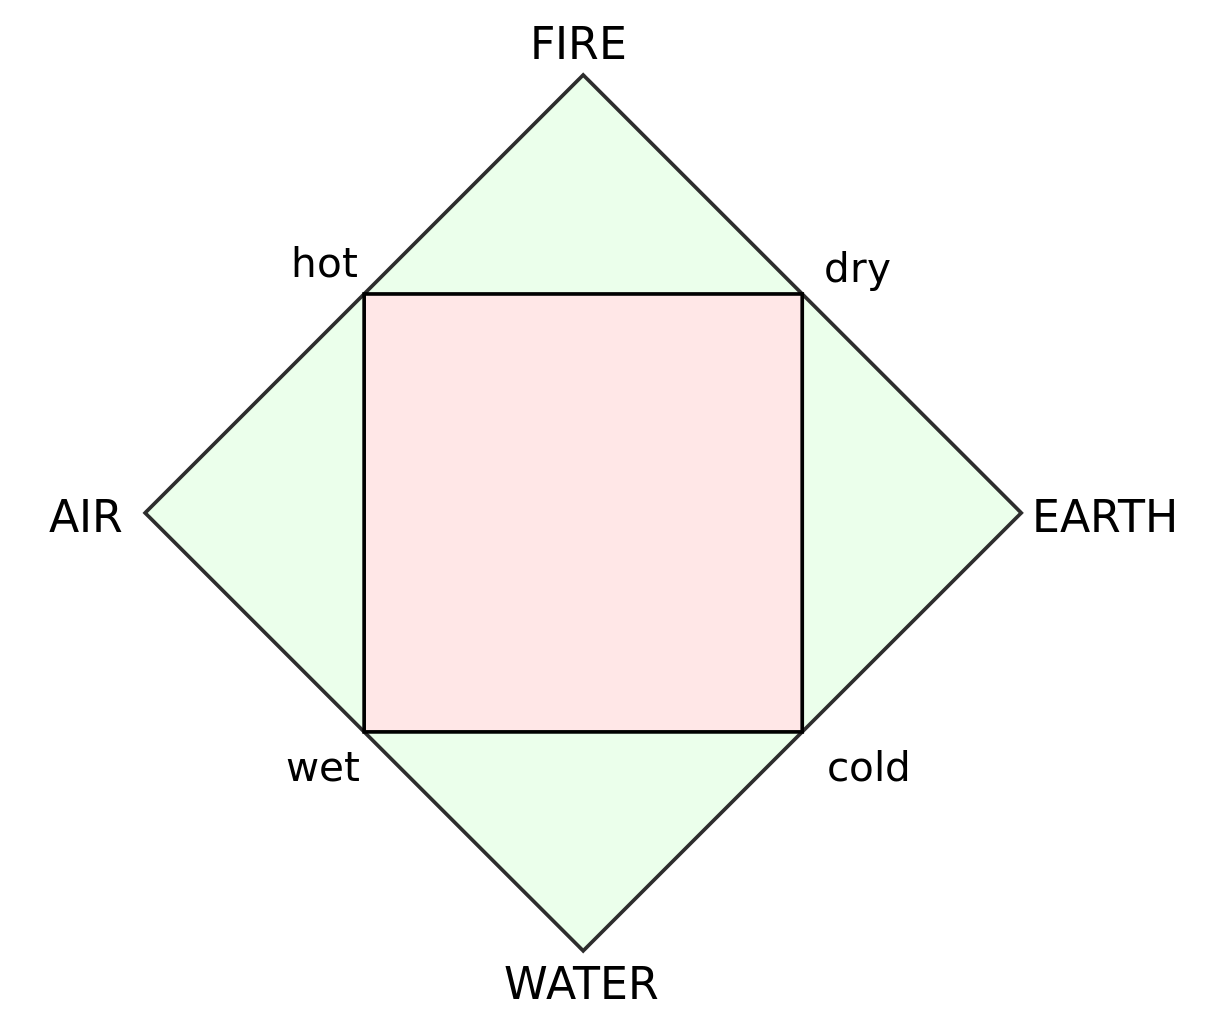
\includegraphics[width=0.90\textwidth]{figures/intro/Four_elements_representation.png}
      \end{center}
\caption{The four roots how they relate to the sensible quantities.}
\label{fig:aristotle}
\end{figure}

Today we have the Standard Model, the theoretical framework that best describes the
experimentally oberserved phenomena of the fundamental particles and their interactions. The theory
is not perfect, and it remains an overarching theme of particle physics to unify physical processes
at all energy scales under one single framework, if such a thing can be done at all.
The SM, its successes, and its shortcomings are described in
Sections~\ref{sec:SM}, \ref{sec:SMsuccess}, and \ref{sec:SMshortcomings}.

Recently in 2012, the last piece to the SM was put into place with the discovery of the Higgs boson.
This discovery, described in Section~\ref{sec:discovery}, is the foundation for the work based on
this thesis, the goal of which is to describe the first search for diHiggs production, a process
in which two Higgs bosons are produced. The motivations for what the search for this process means
in the context of SM physics and ``new'' physics is given in Section~\ref{sec:diHiggs}.

Finally, for those readers who have by chance come across this thesis and do not
have any physics training, Appendix~\ref{ch:mom} may be especially appealing.

\section{The Standard Model\label{sec:SM}}

The Standard Model (SM) of particle physics is a relativistic quantum field theory
that describes how the known fundamental particles interact through the electromagnetic, weak,
and strong forces.
The theory was developed through the unification of the electromagnetic and weak forces by Glashow
in 1961~\cite{1961.Glashow.Partial-symmetries} and through the incorporation of this electroweak
theory with the Higgs mechanism by Weinberg and Salam in 1967~\cite{PhysRevLett.19.1264,Salam:1968rm}.
This theory explained the experimental observations of the day, and later experiments provided
additional evidence as well as a mean for measuring the free parameters of the theory. Some of
this evidence is provided in Figure~\ref{fig:discoveries} in the form of the discoveries of
the fundamental particles.

\begin{figure}[ht]
 \begin{center}
    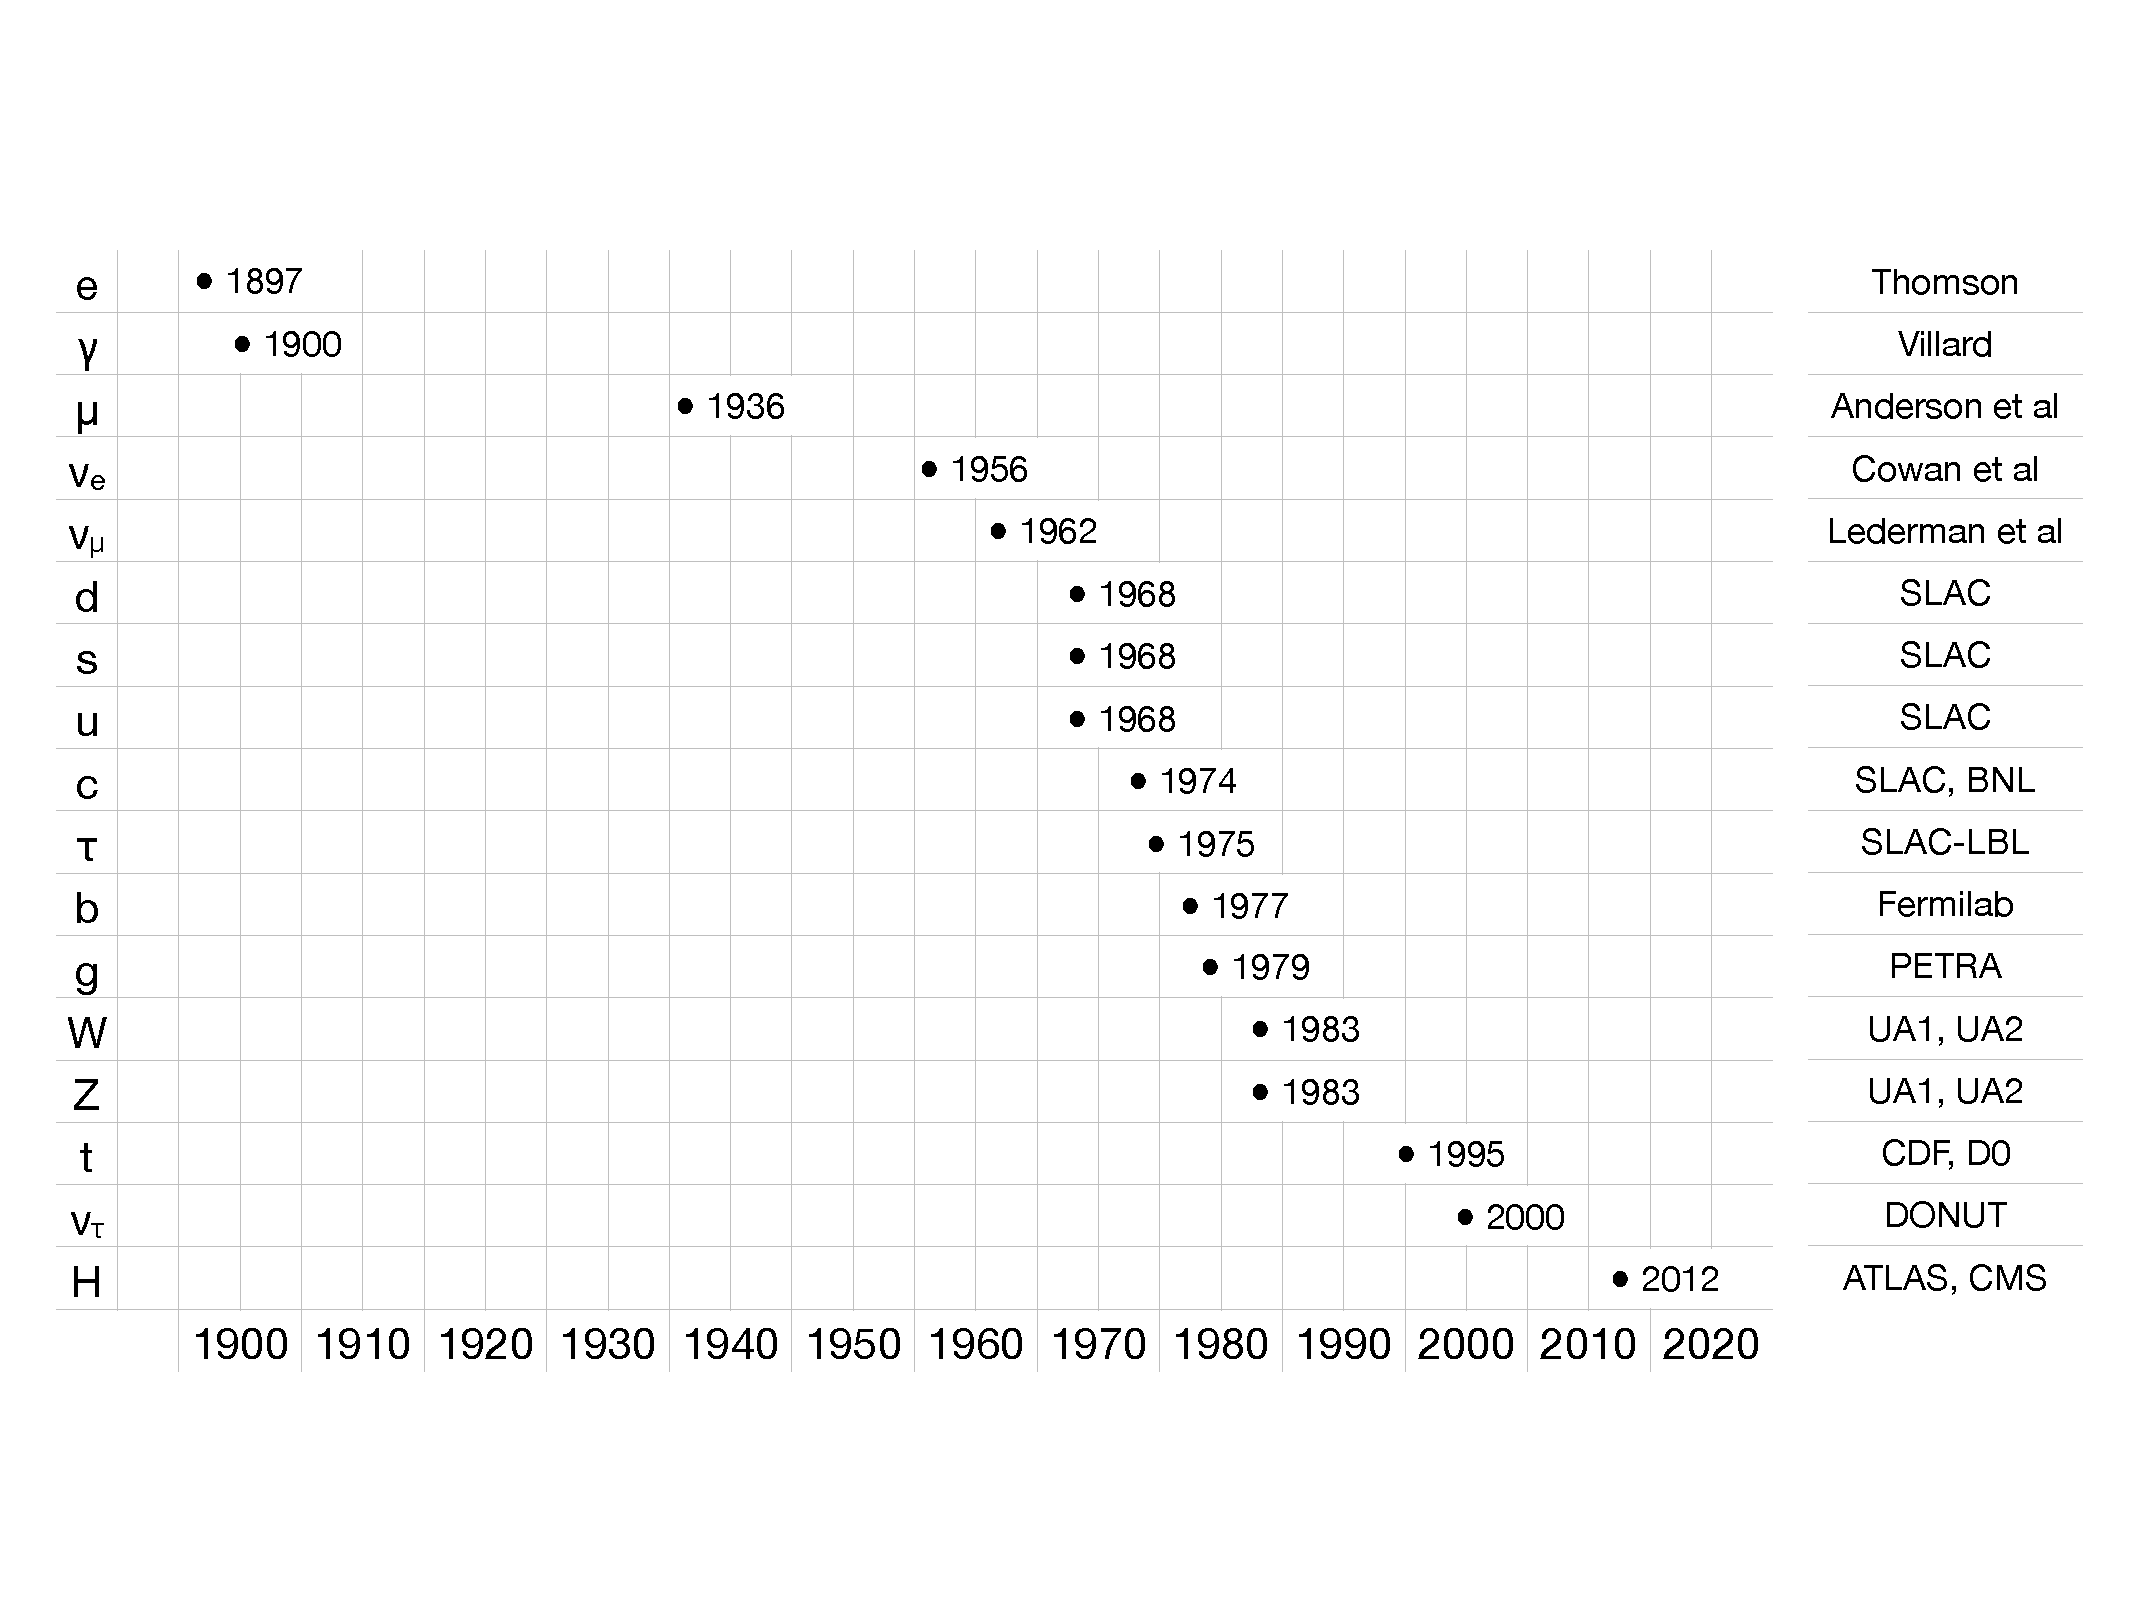
\includegraphics[width=0.90\textwidth]{figures/intro/discoveries.pdf}
      \end{center}
\caption{The discoveries of fundamental particles versus time~\cite{Tuna:thesis}.}
\label{fig:discoveries}
\end{figure}

In this theory, particles are treated as excitations of fields having half-integer spin or
integer spin, and the forces are treated as interactions among excitations of these fields.
The spin-$\frac{1}{2}$ particles, or fermions, can be divided into groups based on the ways
in which they interact. The leptons, or those particles which only experience the electroweak force,
are the electron $e$, muon $\mu$, tau $\tau$, electron neutrino $\nu_e$, muon neutrino $\nu_\mu$, and
tau neutrino $\nu_\tau$. The quarks, or those particles which experience both electoweak and strong
forces, are the up $u$, down $d$, strange $s$, charm $c$, bottom $b$, and top $top$. The integer-spin
particles, or bosons, are the spin-1 photon $\gamma$, $W$, $Z$, and gluon $g$ and the spin-0 Higgs $H$.
The particle content of the SM is summarized in Figure~\ref{fig:SMtable}.

\begin{figure}[ht]
 \begin{center}
    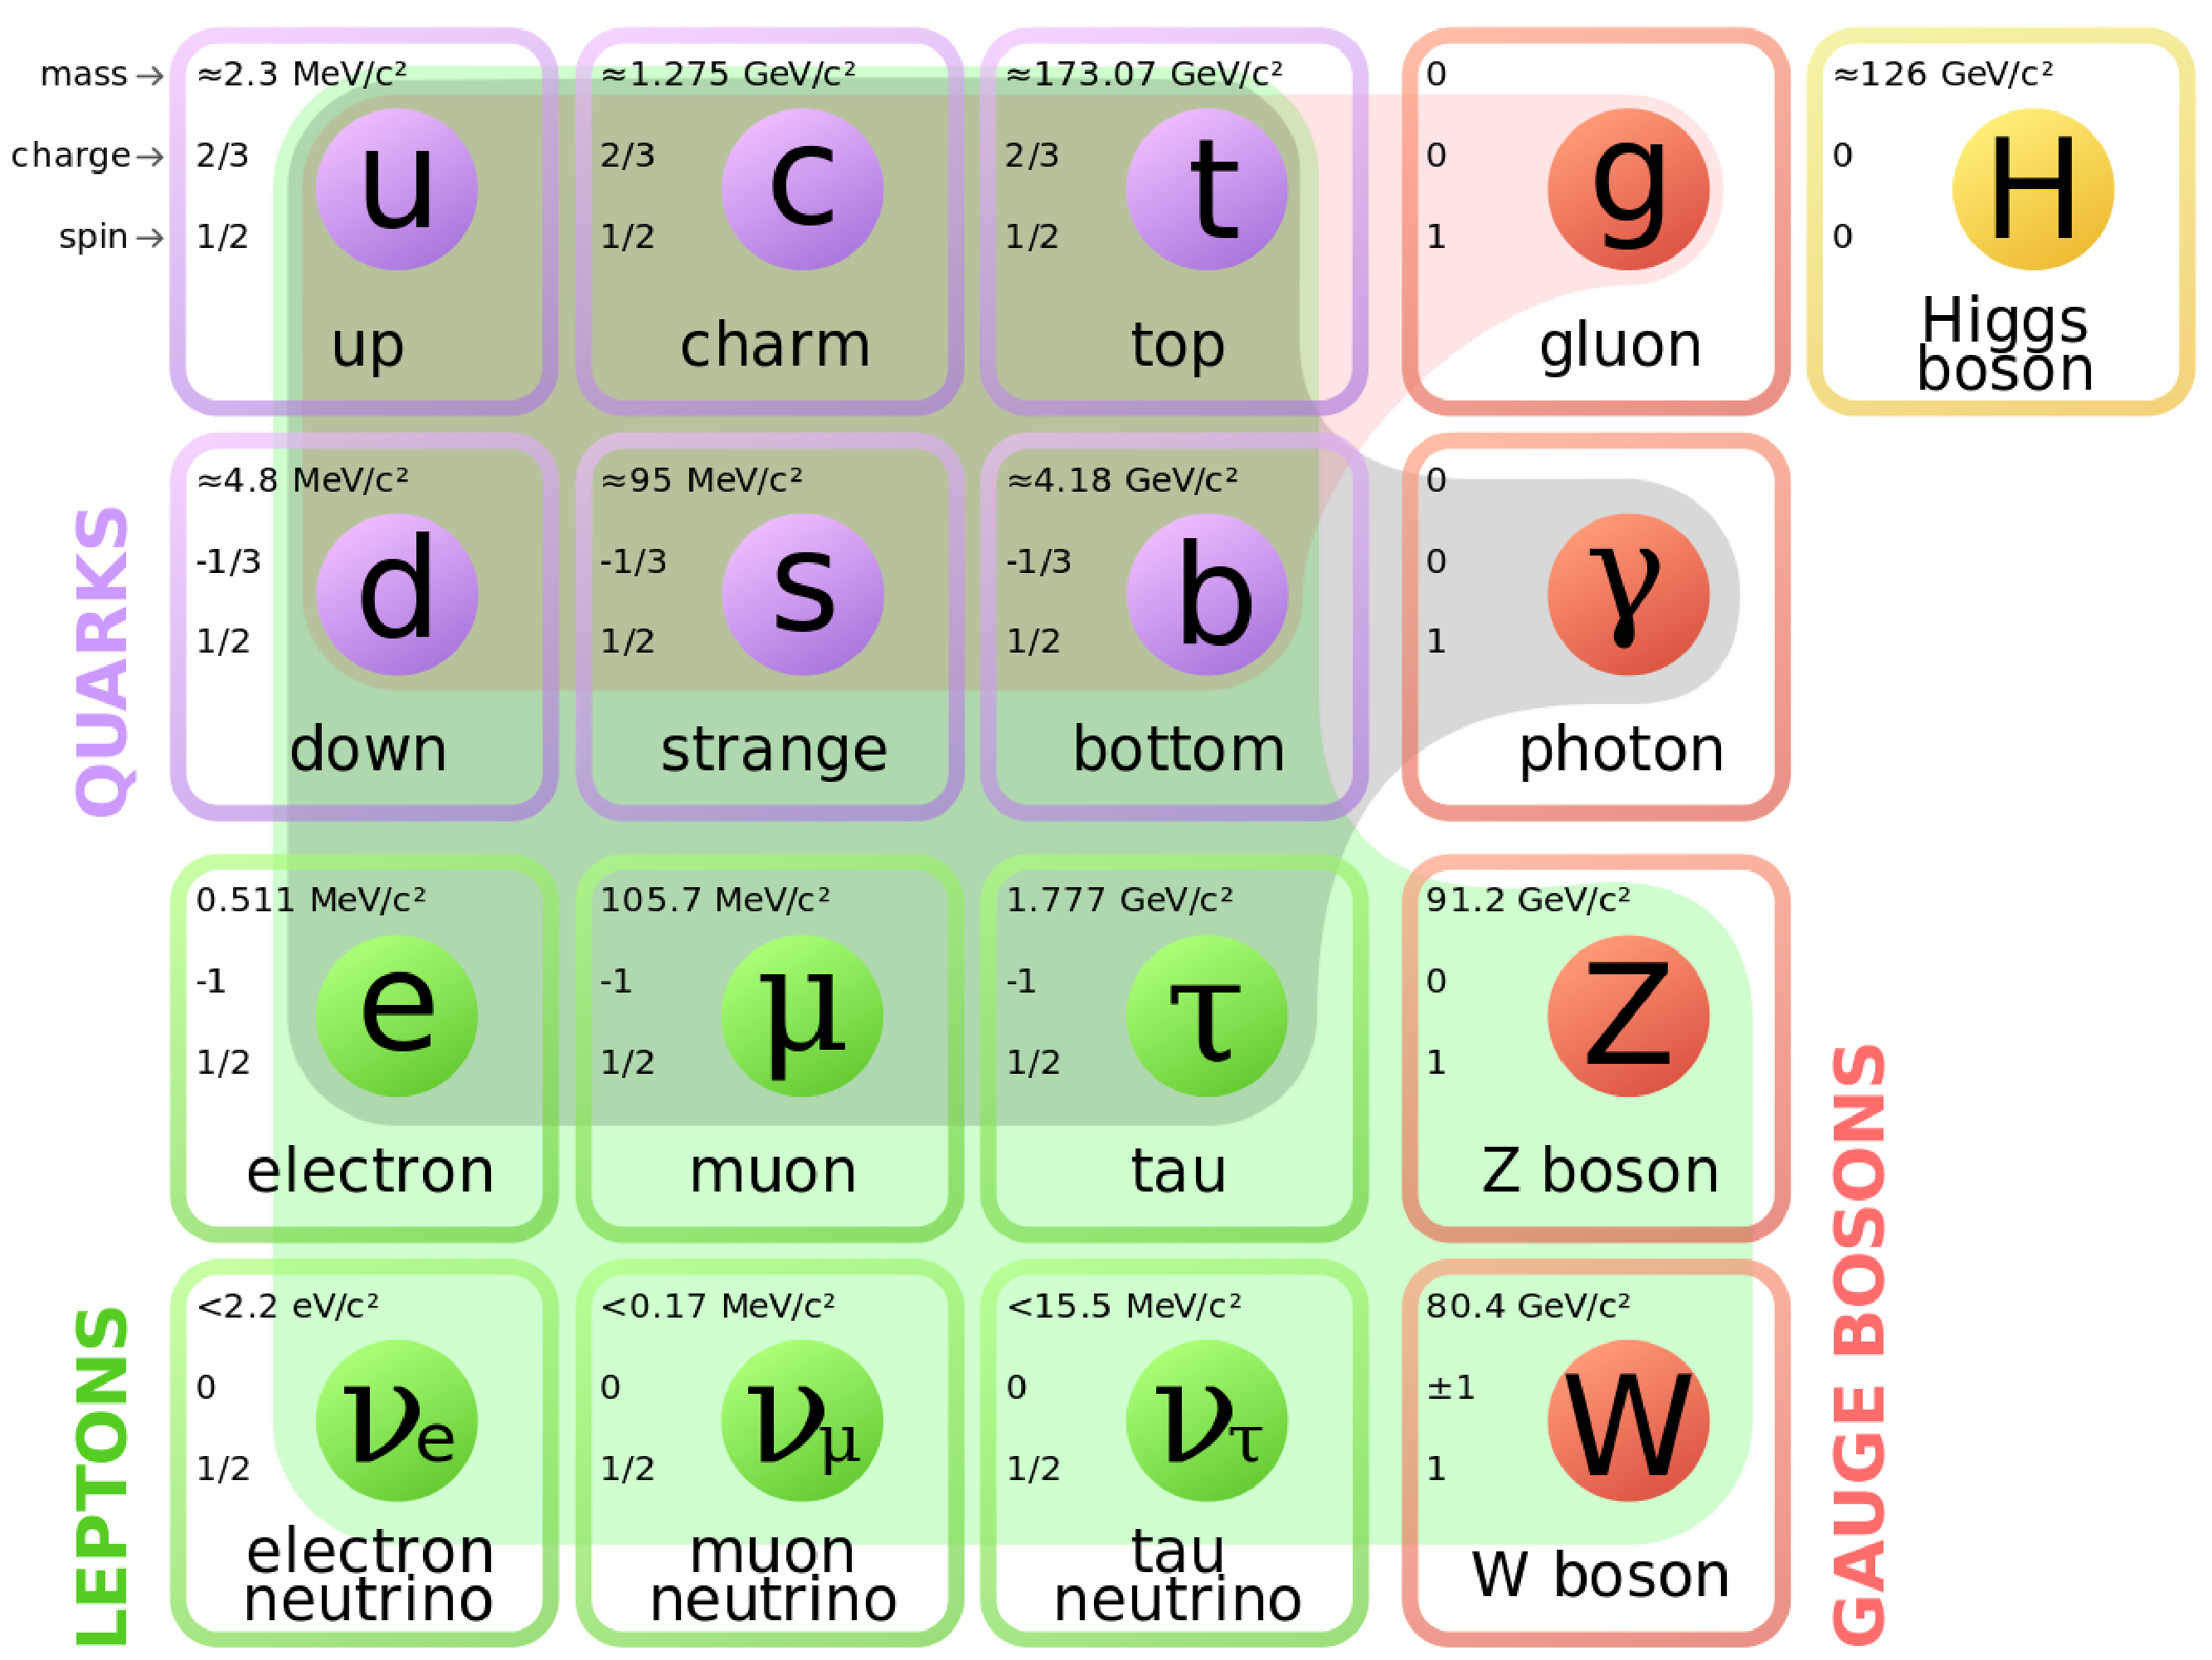
\includegraphics[width=0.90\textwidth]{figures/intro/Standard_Model_of_Elementary_Particles_modified_version.pdf}
      \end{center}
\caption{A diagram of the particle content of the SM~\cite{SMdiagram}.
The mass, electric charge, and spin is given for each, and the background color indicates how each
fermion interacts with the bosons.}
\label{fig:SMtable}
\end{figure}

The dynamics of the SM are described through its Lagrangian, which is invariant under
gauge transformations of the group $\text{SU(3)}_C \times \text{SU(2)}_L \times \text{U(1)_Y}$.
The strong force is associated with transformations under $\text{SU(3)}_C$, which give rise to
the conserved color charge $C$, denoted red, green, or blue, and eight gauge fields.
The group acts on 18 spinor fields corresponding to the quarks (six quark flavors in three colors)
and the eight gauge fields corresponding to the gluons.
The electroweak force is associated with transformations under $\text{SU(2)}_L \times \text{U(1)_Y}$,
the first part of which give rise to the conserved left-handed chirality $L$ and three gauge fields,
and the second part of which gives rise to the conserved weak hypercharge $Y$ one gauge field.
This group acts on left-handed doublets and right-handed singlets of the quarks, leptons, and
these four gauge fields. The quarks contribute nine doublets and 18 singlets, and the leptons contribute
three doublets and three singlets (as right-handed neutrinos do not exist).

The symmetry group of the SM does not allow for gauge-invariant mass terms. Instead,
the generation of particle masses is accomplished through the partial breaking of the
symmetry group by the addition of the Higgs field and potential, after which gauge-invariant
Yukawa interactions between fermions and the Higgs field naturally give fermion masses.
The Higgs field is a doublet of $\text{SU(2)}_L$. blah


\section{Higgs Discovery\label{sec:discovery}}
reference by sec:CMS

\section{Successes of the SM\label{sec:SMsuccess}}

\section{Shortcomings of the SM\label{sec:SMshortcomings}}
reference by sec:CMS


\section{diHiggs as a probe of SM and New Physics\label{sec:diHiggs}}



\chapter{Theory}

\section{Standard Model of Particle Physics}

It is the goal of this section to succinctly (in a relative sense) derive the standard model of particle physics from 
fundamental principals of minimal action, dimensional analysis, symmetry, renomalizability and energy.
First we will describe the lagrangian formulation of classical mechanics. From here we introduce, 
classical field theory and the fundmantal quantization of quantum mechanics to arrive at quantum field
theory (QFT). After a brief discussion of global and local lagrangian symmetries in a QFT, we discuss
gauge theories and how local gauge symmetries give rise to the interactions mediating the 
fundamental forces excluding gravity. Ultimately, we review spontaneous 
electroweak symmetry breaking as the source of the gauge boson masses and the higgs field. 

\subsection{Getting to Quantum Field Theory}

\subsubsection{Lagrangian Mechanics}

In lagrangian mechanics, the time evolution of some generalized coordinate $q$ can
 be determined via the principle of minimal action $\delta S = 0$. 
\begin{align*}
S[q(t)] &= \int_{t_1}^{t_2} L \left(q,\frac{dq}{dt},t\right) dt
\end{align*}
where $S$ is a functional of the time dependent generalized coordinate $q(t)$. 
Let $\dot{q} = \frac{dq}{dt}$ The equations of motion are derived by varying S
\begin{align*}
\delta S &= \int_{t_0}^{t_1} \left [ \frac{\partial L}{\partial \dot q}  \delta \dot q + \frac{\partial L}{\partial q} \delta q \right ]dt 
\end{align*}
Note that $\delta \dot q = \delta\frac{dq}{dt} = \frac{d(\delta q)}{dt}$. 
Integrate the first term by parts, and require that $\delta q$ vanish at the boundaries:
\begin{align*}
\int_{t_0}^{t_1} \left [-\frac{d}{dt}\left (\frac{\partial L}{\partial \dot q} \right) \delta q + \frac{\partial L}{\partial q} \delta q \right ] dt  = \delta S = 0
\end{align*}
by the principle of minimal action we have arrived at the euler equations of motion:
\begin{align*}
\frac{d}{dt}\left (\frac{\partial L}{\partial \dot q} \right) = \frac{\partial L}{\partial q}  
\end{align*}
For a generic lagrangian with potential energy term $V(q)$, $L=\frac{1}{2}m_q \dot q^{2} - V(q)$  we obtain the equation of motion (or force law) $F=m\ddot{q}=-\frac{dV}{dq}$ 
\subsubsection{Classical Field Theory}
In comparison with classical mechanics, which deals with finitely many [cite:tong] general
 coordinates $q_i$, classical field theory deals with an infinite number of degrees of freedom 
$\phi_i(\vec x, t)$ [cite:tong] with a degree of freedom for each spatial coordinate  $\vec x,t$ and 
and index $i$. For simplicity we use a single index $\mu$ for the four spacetime dimensions and utilize
the einstein summation convetion where repeated indicies are summed over. 
The corresponding action can be written in terms of a lagrangian density $\mathcal{L}(\phi,\partial_\mu \phi)$
\begin{align*}
S = \int dt L = \int d^3x \int dt \mathcal{L}(\phi,\partial_\mu \phi) = \int dx^4 \mathcal{L}(\phi,\partial_\mu \phi)
\end{align*}
Similarlly, we arrive at classical Euler-Lagrange Equations of motion:
\begin{align*}
\partial_\mu \left( \frac{\partial\mathcal{L}}{\partial (\partial_\mu \phi)}\right) = \frac{\partial \mathcal{L}}{\partial\phi}
\end{align*}
We now consider the simple free lagrangian density for a real scalar field $\phi$:
\begin{align*}
\mathcal{L} = \frac{1}{2}\partial_\mu \phi \partial^\mu \phi - \frac{1}{2} m\phi^2 
\end{align*}
we have achieved a relativistically invariance for free as all indicies are contracted. To see this, consider a lorrentz transformation $\Lambda$ on the kinetic term. The transformation induces $\phi(x) \rightarrow \phi'(x) = \phi(\Lambda^{-1} x) = \phi (y)$. The transformation is $\Lambda$ as we actively
rotate the coordinate system rather than rotating the field. 
\begin{align*} 
\partial_\mu \phi \partial^\mu \phi \rightarrow& ((\Lambda^{-1})^\mu_\rho \partial^\rho \phi)( (\Lambda^{-1})_\mu^\nu \partial_\nu \phi) \\
&= \eta^{\rho\nu} \partial_\rho \phi \partial_\nu \phi \\
&= \partial^\nu \phi \partial_\nu \phi 
\end{align*}
where we have used the fact that the the spacetime metric is invariant under a lorentz transformations.
\begin{align*}
\Lambda^\mu_\rho \eta^{\rho \lambda} \Lambda_{\lambda}^\nu = \eta^{\mu\nu}
\end{align*}
As the action integrates over all space time, the change of variable from $x\rightarrow y$ is
inconsequential and yield the same equations of  motion.
Applying the euler lagrange equation we arrive at the 
classical relativistcally invariant klein gordon equation:
\begin{align*}
(\partial^2 - m^2 ) \phi = 0
\end{align*}
taking the fourier transform of state $\phi$:
\begin{align*}
\phi(\vec x, t) = \int \frac{d^3p}{(2\pi)^3} e^{-i \vec p \cdot \vec x } \phi (\vec p, t)
\end{align*}
Note that the $(2\pi)^3$ is a normalization convention on the field. We see that the solution satsifies:
\begin{align*}
\left( \frac{\partial^2 }{\partial t^2} + (p^2 + m^2) \right ) \phi(\vec p, t)= 0
\end{align*}
From this we recognize that this is just the equation of motion for
 a harmonic oscillator with energy $\omega^2 = p^2 + m^2$

\subsubsection{The Canonical Quantization}

Quantum mechanics consists of 4 fundamental postulates. Here we enumerate their classical counter parts [cite.schrednicki]

\begin{enumerate}
\item \textbf{Particle State}: In classical mechanics a the state of a particle is determined by two variables $x(t)$ and $p(t)$. In quantum mechanics, the state is a a vector $|\psi \rangle$ in a hilbert space $\mathcal{H}$
\item \textbf{Dynamic Variables }: Clasically, all dynamical variables are a
 function only $x(t)$ and $p(t)$. In quantum mechanics, classical variables 
represented as a function of $x$ and $p$ are instead 
represented by hermitian operators $X$ and $P$ that statisfy the commutation 
relation $[X,P] = \frac{i}\hbar$. 
\item \textbf{Measurement}: Clasically, the particle state is unaffected by measurement and strictly
deterministic based on the values of $x$ and $p$. Quantum mechanically, a particle in a state $|\psi \rangle$ when measured will yield and eigenvalue $\omega$ of the operator $\Omega$ with probability
$|\langle\omega|\psi \rangle|^2$. After measurement the particle state is the corresponding eigenvector  $|\omega\rangle$
\item \textbf{Time Evolution}: Classically, $p$ and $x$ change with time according to hamiltons (or lagrangian) equations of motion. Quantum mechanics asserts the state vector evolves with time according to the
Schrodinger equation: $i \hbar \frac{d}{dt}|\psi(t) \rangle = H | \psi(t) \rangle$. Where $H$ is the 
hamiltonian with classical $p$ and $q$ replaced by the corresponding quantum mechanical operators
\end{enumerate}

The canonical quantization consists of the second postulate that that measurement of postition
and momentum do not commute (postulate 2). This is the source of the famous heisenburg uncertainty
principle that there are no simultaneously measurable states of $p$ and $q$. 

If we consider the quantum harmonic oscillator with hamiltonian:
\begin{align*}
H = \frac{p^2}{2} + \frac{1}{2}\omega^2 q^2
\end{align*}
and postulate the existance of the creation ($a^\dagger$) and annihilation ($a$) operators:
\begin{align*}
a &= \sqrt{\frac{\omega}{2}}q + \frac{1}{\sqrt{2\omega}}p \\
a^\dagger &= \sqrt{\frac{\omega}{2}}q - \frac{1}{\sqrt{2\omega}}p 
\end{align*}
which corresponding give the 
\begin{align*}
q = \frac{1}{\sqrt{2\omega}} (a + a^\dagger)\\
p = -i \frac{\omega}{2}( a - a^\dagger) 
\end{align*}
 substituting into the hamiltonian we find a simple solution after applying
the commutation relation $[p,q]=-i$ (where we have set $\hbar=1$):
\begin{align*}
H =  \omega(a^\dagger a + \frac{1}{2}) 
\end{align*}
Importantly we see via the relation $[H,a]|E\rangle = (E-\omega)a|E\rangle$ and 
$[H,a^\dagger]|E\rangle = (E+\omega)a^\dagger|E\rangle$ that the operators raise and 
lower the harmonic oscillator in multiples of $\omega$. The energy levels are quantized 
in units of $\omega$. Also called ladder operators, $a$ and $a^\dagger$, raise and lower
the energy state by 1 unit of $\omega$ with a ground state energy $\frac{\omega}{2}$. 

If we now consider knowledge of classical field theory we can build a quantum field by
promoting the coordinate $q$ to a field $\phi$. We now write
the solution to the Klein-Gordon equation as an infinite sum of creation and 
annihilation operators that create or destroy a particle with energy $\omega_p^2 =
p^2 + m^2$ designated by its four-momentum $p$. Taking the solution to fourier space:
\begin{align*}
\phi = \int d^4x \frac{1}{\sqrt{2\omega_{p}}} \left [  a_p e^{ipx} + a_p^\dagger e^{-ipx} \right ]
\end{align*} 

Although result only applies for a real scalar field (spin 0), the corresponding feminoic field (spin 1/2)
field can be found similarlly starting from the dirac equation. 

\subsection{Symmetries}

\textbf{Noether's Theorem}

It cannot be understated the importance and the consequences of symmetries in the standard model. The
invariance of the action (equivalently the equations of motion) under linear translations of the  coordinates
gives rise to conservation of momentum. Simillarly,  rotations of the coordinate space
yields the conservation of angular momentum. This is a consequence of noether's theorem, that every 
continuous symmetry of the action has a corresponding conservation law. 

To be concrete, let us consider an action that is invariant under some field transformation
 $\phi \rightarrow \phi + \delta \phi$. If we consider a gauge transformation $\phi \rightarrow e^{i \beta}\phi$  
then the infinitesimal transformation is $\delta \phi = i \beta \phi$. Where we are taking for granted that $\delta S =0$ under
this variation, or effectively $\delta \mathcal{L}$ up to surface terms in the action integral. More on this later.
\begin{align*}
\delta \mathcal{L} &=  \left [ \frac{\partial \mathcal{L}}{\partial \phi} \delta \phi  + \frac{\delta \mathcal{L}}{\partial_\mu (\partial_\mu \phi)} \delta(\partial_\mu \phi) \right]\\
&= i\beta \left [ \frac{\partial \mathcal{L}}{\partial \phi}  \phi  + \frac{\partial \mathcal{L}}{\partial (\partial_\mu\phi)} (\partial_\mu \phi) \right]
\end{align*}
We futher require that the solution satisfying the euler-lagrange equations, and exchange the first term:
\begin{align*}
&= i\beta \left [ \partial_\mu \frac{\partial \mathcal{L}}{\partial(\partial_\mu \phi)}  \phi  + \frac{\partial \mathcal{L}}{\partial_\mu \phi} (\partial_\mu \phi) \right]\\ 
&= i\beta \left [ \partial_\mu  \left [  \frac{\partial \mathcal{L}}{\partial(\partial_\mu \phi)}   \phi  \right ] \right ]\\ 
&= \partial_\mu \left [ \frac{\partial \mathcal{L}}{\partial (\partial_\mu \phi) }\right ] \\
\partial_\mu j^\mu &= 0 
\end{align*}
Where $j^\mu$ is the conserved current corresponding to the continuous symmetry. Now consider the consequences for fermonic lagrangian:
\begin{align*}
\mathcal{L} = \bar{\psi}(i \gamma^\mu \partial_\mu -m)\psi
\end{align*}
the corresponding current is $j^\mu = i\bar \psi \gamma^\mu \psi = (\rho, \vec j)$ where $\rho$ is charge density and $\vec j$ is electric current.
We expand the index and $\partial_\mu = (\frac{d}{dt}, \vec \nabla)$ we obtain the continuity equation:
\begin{align*}
\frac{d\rho}{dt} + \nabla \cdot \vec j = 0
\end{align*}

\textbf{Symmetry Groups and Algebras}

cite.groups.resp.and.physics.HF.jones

To describe symmetry mathematically we need to discuss groups. A group
is an algebraic structure (the field of math is known as abstract algebra and more specifically group theory) that 
consists of a set $G$ (ex. Integers) and a pairwise operation (ex. multiplication) $a\cdot b = c$ where $a,b, c\in G$.
The group must also contain an identity $i \in G$ (ex. 1) such that $i\cdot g = g$ for all $g\in G$. All elements 
$g\in G$ must have an inverse $g^{-1} \in G$ such that $g \cdot g^{-1} = g^{-1} g = i$. The operation must additionally
satisfy associativity $(a\cdot b) \cdot c = a \cdot (b \cdot c)$. Importantly, the group does not necessarily 
need to be abelian $a\cdot b = b \cdot a$, a common example in physics is generic matrix multiplication.

For example, we can consider the group of rotations $SO(3)$ (read special orthogonal group of
dimension 3) about the origin in euclidian $\mathbb{R}^3$ under composition. Clearly the composition
of two rotations is another rotation, the inverse rotation is just rotatating back, and the identity is
not rotation at all. The rotations can be represented by real 3 by 3 matrices, determinant $\pm 1$, 
where element inverses are their transpose $g^{-1}=g^T$. Interestingly, the group $SU(2) \cong SO(3) / \mathbb{Z}_2$, that is, 
SU(2) is a double covering of $SO(3)$. The isomorphism is exact 

Sepcifically, a lie group is a continuous group with a multaplicative law that is a differentiable function of the parameters. linear combinations of generator elements:
\begin{align*}
e^{-i\vec \beta \cdot \vec T} = e^{-i\beta^i T^i} = U_{G}(\vec \beta)
\end{align*}
where the $T^i$ are the generator elements. 
For instance, we can build rotations in 3 dimensional space 
using the dimension 2 representation by exponentiating the pauli spin matrices $\vec \sigma = (\sigma_1, \sigma_2, \sigma_3)$ 
(note the conventional normalization) :
\begin{align*}
L_1 = \frac{\sigma_1}{2} = \frac{1}{2} \begin{pmatrix} 0 & 1 \\ 1 & 0 \end{pmatrix} \\
L_2 = \frac{\sigma_2}{2} = \frac{1}{2} \begin{pmatrix} 0 & -i \\ i & 0 \end{pmatrix}\\
L_3 = \frac{\sigma_3}{2} =  \frac{1}{2} \begin{pmatrix} 1 & 0 \\ 0 & -1 \end{pmatrix} 
\end{align*}
In fact, generically the lie algrebra of a group $G$ is defined by the commutation relations of its generators $T^i$, 
specifically:
]\begin{align*}
[T^i, T^j] = T^iT^j - T^jT^i=  i c_{ijk} T^k
\end{align*}
where $c_{ijk}$ are known as the structure constants of the algebra. The algebra is abelian 
if and only if all $c_{ijk}=0$. Otherwise, the $c_{ijk}$ must be anti-symmetric in any of the two indicies. 

In particular to quantum field theory, the Poincare symmetry group plays an important role in the 
source of the most fundamental conservation laws and the statistics of the quantum fields. 
The poincare Symmetry group consists of transformations of the form:
\begin{align*}
x'_\mu = \lambda^\nu_\mu x_\nu + a_\mu 
\end{align*}
where $\Lambda^\nu_\mu$ is a lorrentz transformation from the lorrentz group $SO(3,1)$ (boosts and rotations) and 
$a_\mu$ is a translation consisting of 4 single 4-vector $\mathbb{R}^{3,1}$. 

The generators of the Poincare group can be enumerated as generalized angular momentum operators:
$L_{\mu\nu} = i(x_\mu \partial_\nu - x_\nu \partial_\mu)$ with the commutation relations:
\begin{align*}
[L_{\mu\nu}, L_{\rho\sigma}] = -i(\eta_{\mu\rho} L_{\nu \sigma}  - \eta_{\nu \sigma} L_{\nu \rho} + 
\eta_{\nu \sigma} L_{\mu \rho} - \eta_{\nu \rho} L_{\mu \sigma})
\end{align*}
However, by decomposing the operators into rotations and boosts these relations become much simpler. Define:
\begin{align*}
J_i &= \frac{1}{2}\epsilon_{ijk} L_{jk}\\
P_i &= i\partial_i\\
K_i &= L_{0i}
\end{align*}
Where $J$ and $P$ are the familiar angular and linear momentum operators. 
We obtain more familar commutations relations:
\begin{align*}
[J_i, J_j] &= i \epsilon_{ijk}J_k  & [P_0,J_j] &= 0 \\
[P_i,J_j] &= i \epsilon_{ijk} P_k & [P_0, K_i] &= i P_i \\
[P_i,K_j] &= i P_0 \delta_{ij} & 
\end{align*}
For a given lie algebra, the dimension of the representation of the group is physically related to the 
 quadratic casamir. For a given concrete representation $L_n$ for a $n$ dimensional
representation, the quadratic casamir $C_2$ can be writen as:
\begin{align*}
L_n^2 = C_2(L_n)I
\end{align*}
where $I$ is the identity. For example, for the group algebra for rotations $SU(2)$ we define $j$ as $n=2j+1$
and consider the $j=0,1/2,$ and $1$ representations. For $j=0$ we have $n=1$ 
 in which case, the rotation is always
trivial to the state. For $j=1/2$ we have $n=2$ with generators:
\begin{align*}
asdf
\end{align*}

The lorrentz group can futher be decomposed into  $SO(3,1) \cong SU(2) \times SU(2)$
where $SU(2)$ is the group of matrices with determinant $\pm 1$ where the inverses are
 the conjugate transpose: $g^{-1} = (g^{T})^*$. The fundamental fields in the SM
lagrangian are characterized by the four corresponding combinations of $SU(2)$ representations. The (0,0) represnetation 
of $SU(2) \times SU(2)$ corresponds to scalar spin 0 fields $\phi$. The two chiral representations (1/2,0) and (0,1/2)
correspond to fermionic matter fields $\Psi$. The (1/2,1/2) representation corresponds to the fundamental 
vector boson fields $W_\mu, B_\mu, G_\mu$ and the fields after electroweak symmetry breaking. $W^{\pm}, Z^0, A_\mu$. 


Let us now consider a field transformation $\phi_a \rightarrow \phi_a'$ under some lie algebra with
generators $L_i$ such that the transformation is $U_g(\beta)$. Consider the heisenburg picture of quantum mechanics where operators evolve but 
the states remain fixed. 
\begin{align*}
\langle O' \rangle = \langle \psi | U_g^{-1}(\beta) O U_g(\beta) | \psi \rangle\\
O'= U_g^{-1}(\beta) O U^g(\beta)
\end{align*}
we obtain a transformed quantum field:
\begin{align*}
\phi_a' = e^{-i \vec \beta \cdot \vec T} \phi_a e^{-i \vec \beta \cdot \vec T}
\end{align*}
expanding the exponentials we see that:
\begin{align*}
\phi_a' = \phi_a - i [ \vec \beta \cdot \vec T, \phi_a] + \frac{(-i)^2}{2}[ \vec \beta \cdot \vec \tau, [ \vec \beta \cdot \vec T, \phi_a]] + O(\beta^2)
\end{align*}
Where $L^i$ is the concrete representation of $T^i$. applying $[T^i, \phi_a] = - L_{ab}^i \phi_b$ gives the field transformation law:
\begin{align*}
\phi_a' = \left (e^{i \vec \beta \cdot \vec T} \right)_{ab} \phi_b 
\end{align*}
and similarlly the conjugate field $\phi^\dagger_a$ transforms in the adjoint represention:
\begin{align*}
\phi_a^\dagger = \left( e^{i \vec \beta \cdot \vec T} \right)_{ab} \phi^\dagger_b 
\end{align*}

\textbf{Local Gauge Invariance and the Covariant Derivative} 

cite-peskin-pg482
Lets consider what happens when we promote the lagrangian symmetry of fields under the Standard Model gauge symmetries
to a local symmetry. Local in the sense that a space dependent transformation   for example, the $U(1)$ gauge symmetry transforms the field $\psi$ as:
\begin{align*}
\psi(x) \rightarrow e^{- \alpha(x)} \psi(x)
\end{align*}
If we then consider a direction derivative in the direction $n^\nu$ as defined:
\begin{align*}
n^\mu \partial _\mu \psi (x) = lim_{\epsilon\rightarrow 0} \frac{\psi(x + \epsilon n) - \psi(x)}{\epsilon}
\end{align*}
This is not going to have a simple transformation law, since the two states are not at the same
point in sample time. We need a connection such that we have a simple transformation law. Consider:
\begin{align*}
n^\mu \partial _\mu \psi (x) = lim_{\epsilon\rightarrow 0} \frac{1}{\epsilon} \left ( \psi(x + \epsilon n) - U(x+\epsilon n, x) \psi(x) \right)
\end{align*}
where $U(x,y)$ is our connection and transforms as:
\begin{align*}
U(x,y) \rightarrow e^{i\alpha(x)} U(x,y) e^{-i\alpha (y)}
\end{align*}
such that when we apply the transformation  to the directional derivative we obtain:
\begin{align*}
n^\mu \partial _\mu \psi (x) = lim_{\epsilon\rightarrow 0} \frac{1}{\epsilon} e^{i\alpha(x+n\epsilon)} \left ( \psi(x + \epsilon n) - U(x+\epsilon n, x) \psi(x) \right)
\end{align*}
Now lets expand the transformation for an infinitesimal $\epsilon$:
\begin{align*}
U(x+\epsilon n, x) \approx U(x,x) + c\epsilon n^\mu A_\mu (x) + O(\epsilon^2)\\
= 1 + c\epsilon n^\mu A_\mu (x) + O(\epsilon^2)
\end{align*}
Where we have used the fact that the connection between $x$ and itself is trivial and specificed some arbitrary (but very suggestive of our final answer) constant $c = ie$.
If we would then like to see how this field $A_\mu$ transforms we need to check the $U(x,y)$ transformation:
\begin{align*}
e^{i\alpha(x)} U(x+\epsilon n,x) e^{-i\alpha (y)} &= (1 + i \alpha(x+n\epsilon)) (1-ie\epsilon n^\mu A_\mu)(1 - i \alpha x) \\
&= 1 + i \alpha (x+n\epsilon ) - ie \epsilon n^\mu A_\mu - i\alpha(x)
\end{align*}
comparing this to the expansion of $U(x+\epsilon n, x)$ we see:
\begin{align*}
1 + ie\epsilon n^\mu A_\mu (x) &= 1 + i \alpha (x+n^\mu\epsilon ) - ie \epsilon n^\mu A_\mu(x) - i\alpha(x)\\
A_\mu(x) &=  \left [ \frac{\alpha(x+n^\mu\epsilon) + \alpha(x)}{en^\mu \epsilon} + A_\mu(x) \right] \\
A_\mu(x) &=  \left [ -\frac{1}{n^\mu}\frac{1}{e}\partial_\mu \alpha(x) + A_\mu(x) \right]
\end{align*}
If we pick the axes such that $n^\mu = 1$ then we have the transformation law for the gauge field: $A_\mu(x) \rightarrow A_\mu(x) - \frac{1}{e} \partial_\mu \alpha(x)$.

\subsection{Fundamental Fields and Free Parameters of the Standard Model}
\begin{center}
\begin{table}[]
\begin{center}
\caption{Standard Model particle representations under the symmetry groups $SU(2)$ and $SU(3)$ respectively $n_2$ and $n_3$. Also listed is associated electroweak hypercharge $Y$ as well as the electric charge $Q$ }
\begin{tabular}{cccccccc}
                & $q_L$ & $l_L$  & $u_R$ & $d_R$  & $e_R$ & $\nu_R$ \\
\hline
$n_3$           & 3     & 1      & 3     & 3      & 1     & 1       \\
$n_2$           & 2     & 2      & 1     & 1      & 1     & 1       \\
$Y_{U(1)}$      & 1/6   & $-1/2$ & $2/3$ & $-1/3$ & $-1$  & 0       \\
\hline
\hline
$Q = Y + T_L^3$ & 2/3   & $-1/3$ & 2/3   & $-1/3$ & $-1$  & 0
\end{tabular}
\end{center}
\end{table}
\end{center}


\subsection{Sectors of the Standard Model Lagrangian}
The Standard Model of particle physics consists of a quantum field theory lagrangian with four sectors. and three gauge group symmetries: $U(1)_Y$ hypercharge, 
$SU(2)_L$ left chiral and $SU(3)_c$ color. 
\begin{align*}
\mathcal{L}_{SM} &= \mathcal{L}_{Gauge} + \mathcal{L}_{Fermion} + \mathcal{L}_{Higgs} + \mathcal{L}_{Yukawa}\\
&=\left(-\frac{1}{4} F_{\mu\nu}F^{\mu\nu} \right )
  + \left (\bar\psi i\gamma^\mu \partial_\mu \psi \right) +
 \left(\frac{1}{2}(\partial_\mu \phi)^2 + V(\phi) \right) + \left(\bar \psi_i y_{ij} \psi_j \phi \right ) 
\end{align*}
All standard model particles transform as a multiplet of $SU(3) \times SU(2)_L \times U(1)_Y$.

\textbf{Gauge Sector}

The gauge sector consists of the field stress energy tensor of the 3 corresponding types of gauge bosons:
 $G^i$ (gluons of the color force), $W^i$ ($W$'s of the weak force) and $B$ (of the weak hypercharge). Here the index $i$ enumerates their multiplicity. There are 8 gluons, 3 $W$'s and a single B. Ultimately, we will arrive have 8 gluons, $W^{\pm}$ and the photon $A^\mu$ because the $SU(2)\times U(1)$ 
symmetry is spontaneously broken and the scalar $\phi$ takes on a new vaccum state. More on this later.
\begin{equation}
\mathcal{L}_{Gauge} = - \frac{1}{4} F_{\mu\nu}^{i} F^{\mu\nu i} =  - \frac{1}{4} G_{\mu\nu}^{i} G^{\mu\nu i} - \frac{1}{4} W^{i}_{\mu\nu} W^{\mu\nu i} - \frac{1}{4} B_{\mu\nu}B^{\mu\nu} 
\end{equation}
where the double scripts correspond to the commutation relations for the gauge group algebra. 
\begin{equation}
X_{\mu\nu}^i   = D_\mu X_\nu^i - D_\nu X_\mu^i - g f_{ijk} X_\mu^j X_\nu^k
\end{equation}
where the $D_\mu$ terms correspond to the covariant derivative and the $f_{ijk}$ are the corresponding structure constants for 
non-abelian groups(0 for abelian groups). and $g$ the coupling constant. In full, the field stress tensor terms are:
\begin{align*}
G_{\mu\nu}^i &=  D_\mu G_\nu^i - D_\nu G_\mu^i - g_s f_{ijk} G_\mu^j G_\nu^k\\ 
W_{\mu\nu}^i &=  D_\mu W_\nu^i - D_\nu W_\mu^i - g \epsilon_{ijk} W_\mu^j W_\nu^k\\ 
B_{\mu\nu} &=  D_\mu B_\nu - D_\nu B_\mu
\end{align*}
The fermion sector consists of the kinetic energy terms for each quark (up and down types) and leptons (lepton, neutrinos) in the standard model.
The left handed quarks transform as an SU(2) doublet:
\begin{equation}
q^0_{mL\alpha} = \left( \begin{array}{c} u_{m\alpha}^0  \\ d_{m\alpha}^0 \end{array} \right)_L \text{ and } l_{mL} = \left( \begin{array}{c} \nu_{m}^0  \\ e^{-,0}_{m} \end{array} \right)_L 
\end{equation}
where the subscript $m$ denotes the family (1st, 2nd and 3rd generation) and $\alpha$ denotes the color charge (red, green, and blue).
As the $SU(2)_L$ symmetry only acts on the left handed fermions we further separate the fermion sector into left and right components:
\begin{align*}
\mathcal{L}_{fermion,L} &= \bar{q}^0_{mL} i \gamma^\mu D_\mu q^0_{mL} + \bar{l}^0_{mL} i \gamma^\mu D_\mu l^0_{mL}\\
\mathcal{L}_{fermion,R} &=  \bar{u}^0_{mR} i \gamma^\mu D_\mu u^0_{mR} 
+ \bar{d}^0_{mR} i \gamma^\mu D_\mu d^0_{mR} + \bar{e}^0_{mR} i \gamma^\mu D_\mu e^0_{mR} + \bar{\nu}^0_{mR} i \gamma^\mu D_\mu \nu^0_{mR}
\end{align*}

\textbf{Higgs Sector}

The higgs sector consists of terms related to the single scalar field $\phi$

\textbf{Yukawa Sector}

\subsection{Electroweak Symmetry Breaking}

Expanding the kinetic term for the field phi about the vaccum $\langle \phi \rangle = \nu$ in the gauged theory we find:
\begin{align*}
(D^\mu \phi)^\dagger (D_\mu \phi) = \frac{1}{\sqrt{2}} \left (\begin{array}{cc} 0  & \nu \end{array} \right )  \left | \partial_\mu + i g \frac{\tau}{2} \cdot W_\mu + i \frac{g'}{2} B_\mu \right|^2  \frac{1}{\sqrt{2}} \left (\begin{array}{c} 0 \\ \nu \end{array} \right ) 
\end{align*}
Considering only the the square gauge field terms (ignoring the derivative)  we obtain the matrix:
\begin{align*}
\tau \cdot W + g'B_\mu I = \left (\begin{array}{cc} W_{\mu,3} & W_{\mu,1} - i W_{\mu,2}  \\ W_{\mu,1}+ i W_{\mu,2} & - W_{\mu,3} \end{array} \right )
\end{align*}
adding in the diagonal $B_\mu$ terms and taking the square:
\begin{align*}
(D^\mu \phi)^\dagger (D_\mu \phi) = \frac{\nu^2}{8} \left [g^2 (W_1^2 + W_2^2) + (g' B_\mu - g W_{\mu,3})^2 \right]
\end{align*}
Now if we perform a redefinition of the gauge fields into mass eigenstates we arrive at a clean expression:
\begin{align*}
W_{\mu}^{\pm} &= \frac{1}{\sqrt{2}}( W_{\mu,1}  \pm i W_{\mu,2} ) \\
A_{\mu} &= \frac{1}{\sqrt{g^2 + (g')^2}} (g' W_{\mu,3} + g B_\mu)\\
Z_{\mu} &= \frac{1}{g^2 + (g')^2}( g' B_\mu - g W_{\mu,3}) 
\end{align*}
With this substitution, w
\begin{align*}
(D^\mu \phi)^\dagger (D_\mu \phi) &= \frac{\nu^2 g^2}{4} W_{\mu}^{-} W_{\mu}^{+} + \frac{(g+g')\nu^2}{8} Z_\mu^2  + 0 \times A_\mu^2 \\ 
&= \frac{1}{2} m_{W}^2 W_\mu^- W_\mu^+ + \frac{1}{2} m_Z^2 Z_\mu^2  + 0 \times A_\mu^2
\end{align*}
Electroweak symmetry breaking has generated the mass terms for the gauge bosons! $m_Z = \frac{\nu}{2}\sqrt{g+g'} = 91.1876$~[GeV] 
$m_{W^{\pm}} = \frac{\nu g}{\sqrt{2}} = 90.385$~[GeV] and the massless photon $A_\mu$. 

\subsection{Re-deriving Maxwell's Laws} 

After, electroweak symmetry breaking we would like to see that we retain the fundamental laws of electromagnetism. 
Keeping only the terms that contain the field $A_\mu$:
\begin{align*}
\mathcal_{EM} &= -\frac{1}{4}F_{\mu\nu}F^{\mu\nu}  - ie \bar \psi \gamma^\mu A_\mu \psi 
\end{align*}
where by definition $F_{\mu\nu} = \partial_\mu A_\nu - \partial_\nu A_\mu$. Applying the left side of Euler-Lagrange we find:
\begin{align*}
\partial_\mu \left (\frac{\partial \mathcal L}{\partial(\partial_\mu A_\nu} \right) =  
-\frac{1}{2}\partial_\mu \left [ \left (\frac{\partial}{\partial(\partial_\mu A_\nu)} \right) F_{\mu\nu} \right ] 
\end{align*}
noting that:
\begin{align*}

\end{align*}


\subsection{The Narrow Width Approximation}

\section{Beyond the Standard Model}

\subsection{Problems with the Standard Model}

\subsection{Supersymmetry}

\subsection{Electroweak Symmetry Breaking in Supersymmetric Theories}

\section{Origins of Long-lived Signatures}

\subsection{Standard Model Particles with Long Lifetimes}

The standard model already includes a variety of particles that can generate
 displaced vertices (Table \ref{tab:mesons} Table \ref{tab:baryons}). 
For example, $B^0 \rightarrow J/\psi K^{*0}$ with $K^{*0} \rightarrow K^+\pi^-$ 
generates a 4 track vertex. Such a vertex is commonly utilized 
in b-tagging. Of particular interest to single displaced jet identification outside of the b-tagging regime are charge neutral SM particles
decaying to charged particles with a few centimeter lifetime: $\Lambda^0$, $K_S^0$. Such particles would have no track
leading to the primary vertex and vertices far outside the b lifetime. The most relevant of processes being:

\begin{enumerate}
\item $K_s^0 \rightarrow \pi^+\pi^-$ 69\% of all $K_s^0$ decays 
\item $\Lambda^0 \rightarrow p \pi^-$ 64\% of all $\Lambda^0$ decays 
\end{enumerate}

Jets containing prompt and non-prompt $K_s$ and $\Lambda^0$ will contain tracks with large impact parameters, 
and large impact parameter significance. When a vertex is fit to the matched tracks we expect small track multiplicity relative 
to the GeV to TeV   long-lived particles this identification targets. It is important to separate this contribution from
the detector effects like nuclear interactions.

\begin{table}
\begin{center}
\begin{tabular}{cccccc}
\hline
\textbf{Name}  & \textbf{Content}                                    & \textbf{Particle}    & \textbf{mass} (MeV) & $\tau_{0}$ (sec)  & c$\tau$ (cm)         \\
\hline 
Pion & $u\bar{d}$                                  & $\pi^{\pm}$ & 139        & $2.6 \times 10^{-8}$       & $7.8 \times 10^{2}$  \\
\hline 
Kaon  & $u\bar{s}$                                 & $K^{\pm}$   & 497        & $     1.23 \times 10^{-8}$ & $3.7 \times 10^2$    \\
K Short  & $\frac{1}{\sqrt{2}}(d\bar{s} - s \bar{d})$ & $K^0_{s}$   & 497        & $0.896 \times 10^{-10}$    & 2.68                 \\
K Long  & $\frac{1}{\sqrt{2}}(d\bar{s} + s \bar{d})$ & $K^0_L$     & 497        & $5.1\times 10^{-8}$        & $1.5 \times 10^3$    \\
\hline
D & $c\bar{d}$                                 & $D^{\pm}$   & 1869       & $1 \times 10^{-12}$        & $3.0 \times 10^{-2}$ \\
\hline
B meson  & $u \bar{b}$                                & $B^{\pm}$   & 5279       & $1.6 \times 10^{-12}$      & $4.8 \times 10^{-2}$ \\
strange B  & $s\bar{b}$                                 & $B^{0}_s$   & 5366       & $1.5 \times 10^{-12}$      & $4.5 \times 10^{-2}$ \\
charmed B  & $c\bar{b}$                                 & $B^{0}_c$   & 6275       & $4.5\times 10^{-13}$       & $1.4 \times 10^{-2}$ \\
\end{tabular}
\end{center}
\caption{Mesons with Lifetimes greater than $10^{-2}$ cm} 
\label{tab:mesons}
\end{table}


\begin{table}
\begin{center}
\begin{tabular}{cccccc}
\textbf{Name}          & \textbf{Content} & \textbf{Particle}      & \textbf{mass} [MeV] &  $\tau_{0}$ [s] & $c\tau_{0}$ [cm] \\
\hline 
Lambda        & $uds$   & $\Lambda^0$   & 1115       & $2.6 \times 10^{-10}$    & 7.8                  \\
bottom Lambda & $udb$   & $\Lambda^0_b$ & 5620       & $1.4 \times 10^{-12}$    & $4.2 \times 10^{-2}$ \\
\hline
Sigma plus    & $uus$   & $\Sigma^{+}$  & 1189       & $8 \times 10^{-11}$      & 2.4                  \\
Sigma minus   & $dds$   & $\Sigma^{-}$  & 1197       & $1.4\times 10^{-10}$     & 4.2                  \\
\hline 
Xi zero       & $uss$   & $\Xi^0$       & 1314       & $4 \times 10^{-13}$      & $1.2 \times 10^{-2}$ \\
Xi minus      & $dss$   & $\Xi^-$       & 1321       & $1.6 \times 10^{-10}$    & 4.8                  \\
charmed Xi +  & $usc$   & $\Xi^{+}_c$   & 2467       & $4.42 \times 10^{-13}$   & $1.3 \times 10^{-2}$ \\
charmed Xi    & $dsc$   & $\Xi^0_c$     & 2471       & $1.12 \times 10^{-13}$   & $3.3 \times 10^{-2}$ \\
bottom Xi     & $dsb$   & $\Xi^-_b$     & 5792       & $1.56 \times 10^{-12}$   & $4.7 \times 10^{-2}$ \\
\hline
bottom Omega  & $ssb$   & $\Omega_b^-$  & 6054       & $1.13 \times 10^{-12}$   & $3.3 \times 10^{-2}$ \\
Omega minus   & $sss$   & $\Omega^-$    & 1672       & $8 \times 10^{-11}$      & 2.4                  \\
\end{tabular}
\end{center}
\caption{Baryons with Lifetimes greater than $10^{-2}$ cm} 
\label{tab:baryons}
\end{table}


Particles of a characteristic lifetime $\tau$ decay with a falling exponential. For reference, 
a table describing the percent of decays that will occur at various distances is shown in Table
 \ref{tab:lifetime}. Even lifetimes 10 and 100 times the size of the tracker, we would still expect
~10\% and 1\% respectively to occur within the tracker. For particles  of lifetime $\lambda$ we
expect 0.6\% to decay beyond $5\lambda$. 


\begin{table}
\begin{center}
\begin{tabular}{ccc}
Distance ($\lambda$) &  Probability of Decay  \\
\hline
0.01               & 1\%                        \\
0.1                & 9.5\%                      \\              
0.25               & 22\%                       \\            
0.5                & 39\%                       \\          
0.75               & 52\%                       \\        
1                  & 63\%                       \\      
1.5                & 77\%                       \\    
2                  & 86\%                       \\  
3                  & 95\%                       \\
5                  & 99.3\%                     \\
\end{tabular}
\end{center}
\caption{ A reference table for the cumulative probability for a particle of lifetime $\lambda$ to have decayed after a given
distance. Distance is in multiples of lambda.}
\label{tab:lifetime}
\end{table}


\subsection{Split-Susy and Naturalness at the LHC}

The expectation of discovering supersymmetry (SUSY) at the TeV scale has been largely motivated
 by arguments based on naturalness. 
Since the mass of the Standard Model Higgs boson is sensitive to the high energy scale where SUSY
 is broken ($m_{SUSY}$), its mass, of order the electroweak scale, $(m_h \approx m_{EW} \ll m_{SUSY})$
 would need to be tuned to order $m_{EW}^2/m_{SUSY}^2$. 
To avoid fine-tuning, we would like  $m_h^2 \approx m_{SUSY}^2 \implies m_{SUSY} \leq$ 1 TeV. 
More specifically, knowing $m_H \approx 125$ GeV we expect light SUSY partners (in particular, light stops)
 near $< 1$ TeV to stabilize the quadratic divergences of 1 loop corrections to the Higgs mass
 [citation:$light_stops$]. 
Unfortunately these scalar partners have yet to be discovered.

It is important to note that the stability of the Higgs boson mass is not the only
 fine-tuning problem in particle physics. 
When the same argument is made for the cosmological constant we arrive at $\Lambda \geq m_{SUSY}^4$, 
where experimentally $\Lambda = 10^{-59}$ TeV$^4$.   
If we use the same SUSY scale as we did for the Higgs mass,
 $m_{SUSY} = 1$ TeV we have a new fine tuning problem of $10^{60}$.

As addressed by Arkani-Hamed and Dimopoulos [citation:$nima_lhc$], many theoretical approaches  have been
 motivated by a natural explanation for the Higgs mass while separately seeking an  explanation
 of the cosmological constant through some other mechanism.
Arkani-Hamed and Dimopoulos propose a reconsideration of naturalness, entertaining the idea that 
fine tuning could have a role to play in beyond the Standard Model physics.
Conceivably, both $\Lambda$ and $m_h$ fine tuning could be resolved by the same mechanism.  
This un-natural model was  further investigated by Giudice and Romanino [citation:$split_susy$]
and dubbed ``split supersymmetry". 

Split SUSY assumes a much higher SUSY scale $m_{SUSY}^2 \gg 1$ TeV where all scalars (excluding the Higgs) 
become very heavy $O(m_{SUSY})$ and the lightest sparticles (Higgsinos and gluinos) are kept at the TeV scale by requiring the lightest neutralino to be a good dark matter candidate. 

Because the scalars are so much heavier, the decay of gluinos through squarks is suppressed.
The characteristic signature of split supersymmetry is thus long-lived gluinos; such processes 
with long lifetimes are rare in the SM.

\chapter{Collider Physics and Phenomenology}

\section{Introduction}

In the previous chapter, we outlined how we reach a theory like the standard model from fundamental principles, but 
a considerable amount of physics is required to reach a practical theoretical description of what occurs inside of 
the experiment. The goal of this section is to connect the matrix elements $\mathcal{M}$ from the quantum field
theoretic description  of the Standard Model to the Monte Carlo simulations used to test a given theory. 
First, we will discuss the how
we can compare the matrix amplitudes with the observations in a physical detector. After, we will the discuss the considerations 
that must be made for the fact the LHC collides hadrons rather than fundamental particles. Finally, we will discuss the framework used to describe the particles actually observed in the detector after the hard scattering occurs where perturbative physics breaks down and  calculations from first principles cannot be performed. Generic principles for parton showering and hadronization models will be examined. 

\section{From Matrix Elements to Cross Sections} 

In high energy experimental particle physics the key quantity (besides particle quantum numbers and masses) is the
cross section $\sigma$ of the process. This is the rate or in essence, the probability that an event occurs. It is the proportionality between the number of observed collisions and the rate at which the Large Hadron Collider delivers collsions $L$ (the luminosity)
 expressed simply as:
\begin{align*}
N_{events} = L \times \sigma
\end{align*}
cite-peskin
Consider a target of particles type $A$ and density $\rho_A$ and aim particles type 
$B$ with density $\rho_B$. If the lengths of the bunches of particles are $l_A$ and $l_B$ 
then the cross section of the processes is defined for a beam with cross-sectional area as:
\begin{align*}
\sigma \equiv \frac{N_{events}}{\rho_A l_A \rho_B l_B A}
\end{align*}
Inverting this and assuming that we have constant density along the beams length:
\begin{equation}\label{eq:sigma}
N_{events} = \frac{\sigma N_A N_B}{A} = \sigma{N_A n_B}
\end{equation}
by comparing this with the relation for $N_{events}$ above containing luminosity, we see the
 luminosity is in effect counting the number of colliding particles per unit area.
 More incident particles and a more focused beam means more scattered events. 
In the last equality we have introduced the impact parameter density $n_B$ for
 the incident $B$ particles.

However, the the end results of feynman diagram calculations yield scattering amplitudes
which are matrix elements of scattering a given intial state into a given final state, not
a cross section. We have to further develop the stocastic interaction of two particles into
something more concrete experimentally.
 
First, we need  must think about the quantum fields within the beams that are colliding. To do so we set up two initial 
wave packets $A$ and $B$ in a limit of definite momentum $p_A$ and $p_B$ and evolve them for a very long time 
with the time evolution operator $\exp{(-iHt)}$ and then consider the final state wave packets with the correct final state particles. This in turn will give us the probability amplitude for producing that final state.  
\begin{align*}
\mathcal{P} = |\langle \phi_1 \phi_2 \ldots| \phi_A \phi_B \rangle | ^2 
\end{align*}
Now consider the number of incident particles colliding along the z-axis, but with non-trivial transverse displacement,
also referred to as impact parameters $b_i$. We will take the perspective that $A$ is a target and $B$ is collinear
with the target and account for the shift in position with an explict factor of $\exp(-ib \cdot k_B)$. The properly normalized expression then reads:  
\begin{align*}
|\phi_A \phi_B \rangle = \int \frac{d^3k_A}{\sqrt{2E_A}(2\pi)^3} \int \frac{d^3k_B}{\sqrt{2E_B}(2\pi)^3}\phi_A(k_A)\phi_B(k_B) e^{-ib \cdot k_B} 
\end{align*}
For a single target $A$ and a beam $B$ with with constant impact parameter density $n_B = N_B / A$ we can write the the number of events as
\begin{align*}
N_{events} = \sum_{\text{incident particles } i} \mathcal{P}_i = \int d^2b n_B(b) \mathcal{P}(b) = n_B \int d^2b \mathcal{P}(b) 
\end{align*}
Comparing this to Equation \ref{eq:sigma} we can write the cross section as:
\begin{align*}
\sigma = \int d^2 b \mathcal{P}(b) 
\end{align*}
and the properly normalized differential cross section for scattering into a the infinitesimal final state momentum element is:
\begin{align*}
 d\sigma &= \left( \prod_f \frac{d^3p_f}{(2\pi)^3 2E_f} \right ) \int d^2b \left ( \prod_{i=A,B}
 \int \frac{d^3 k_i }{(2\pi)^3 \sqrt{2E_i}} \phi_i(k_i) \int \frac{d^3 \bar{k}_i}{(2\pi)^3
\sqrt{2\bar{E}_i}} \phi^*_i(\bar{k}_i) \right)\\ 
 &\times e^{ib\cdot (\bar{k}_S - k_B)} | \langle \{ p_f\} | \{k_i \} \rangle |^2 
\end{align*}
We have 6 dummy integrals to do in $\bar{k}$ over the 3 momentums of particle $A$ and $B$
 so count our delta functions. The $d^2b$ integral gives 2 delta functions in the transverse 
momentum $(2\pi)^2 \delta^2(k_B^\perp - \bar{k}_B^\perp)$.  We have 8 delta functions from 
the matrix element enforcing that the process to conserve energy and momentum
 $\delta^4(k_A +k_B - \sum p_f)$\ and in the complex conjugate with the dummy variable
 $\bar{k}$: $\delta^4(\bar{k}_A + \bar{k}_B - \sum p_f)$. Performing the transverse 
integrals in $\bar{k}_B$ sets $\bar{k}_B^T=k_B^T$ which in combination with the transverse
 barred ampltidue delta functions give $\bar{k}_A^T = k_A^T$. The remaining 2 integrals in $z$ require some properties of delta functions:
\begin{align*}
\int d \bar{k}_A^z d \bar{k}_B^z \delta( \bar{k}^z_A + \bar{k}^z_B  - \sum p_f^z) \delta (\bar{E}_A + \bar{E}_B - \sum E_f) 
\end{align*}
We can integrate the first $B$ integral considering $\bar{k}_B^z$ to be a function of
$\bar{k}_A^z$ and writing the barred energy terms in the momentums and masses:
\begin{align*}
\int d\bar{k}_A^z  \delta \left (\sqrt{\bar{k}_A^2 +m_A^2}  + \sqrt{\bar{k}_B^2 + m_B^2} - \sum E_f \right) 
\end{align*}
We now need to use the property that $\delta[f(x)] = \sum_i (\delta(x_i) / |f'(x_i))|$ where $x_i$ are the zeros of the fuction $f(x)$. Note that given our parmeterization from the first delta function $\partial_{\bar{k}_A^z}(\bar{k}_B^2) = - 2 \bar{k}_B^z$.
\begin{align*}
\int d\bar{k}_A^z & \left (\frac{1}{2} \frac{2\bar{k}_A}{\sqrt{\bar{k}_A^2 +m_A^2}}
 - \frac{1}{2} \frac{2\bar{k}_B}{\sqrt{\bar{k}_B^2 +m_B^2}} \right )^{-1}\delta(\bar{E}_A
 + \bar{E}_B - \sum E_f) \\
=& \int d\bar{k}_A^z \frac{1}{\frac{\bar{k}_A}{\bar{E}_A}- \frac{\bar{k}_B}{\bar{E}_B}}
 \delta(\bar{E}_A + \bar{E}_B - \sum E_f) = \frac{1}{\beta_A - \beta_B}
\end{align*}
The 6 remaining integrals in $k_A$ and $k_B$ remain:
\begin{align*}
d\sigma &= \left( \prod_f \frac{d^3p_f}{(2\pi)^3 2E_f} \right ) \frac{|\mathcal{M}|^2}{2E_A2E_B|\beta_A - \beta_B|}
 \int \frac{d^3 k_A }{(2\pi)^3 \sqrt{2E_i}} |\phi_A(k_A)|^2 \\ 
&\times  \int \frac{d^3 k_B }{(2\pi)^3 \sqrt{2E_i}} |\phi_B(k_b)|^2 \delta^4( k_A + k_B - \sum p_f)
\end{align*}
To proceed further, we must consider the quality of measurements made by particle detectors. 
Real detectors cannot measure arbitrarily small spreads in the momentums $k_A+k_B$. 
The measurements made in a realistic experimental setup are not senitive to the
spread of momentum in the initial wave packets $\phi_A$ and $\phi_B$. Given this, we can take the central value $k_A+k_B=p_A+p_B$
to be a good approximation for the delta function. With this approximation, we can move the delta function outside the integral and
perform the integrals using the unit normalization condition of the two fields $\phi_i$:
\begin{equation} \label{eq:dsigma}
d\sigma = \left( \prod_f \frac{d^3p_f}{(2\pi)^3 2E_f} \right ) \frac{|\mathcal{M}|^2}{2E_A2E_B|\beta_A - \beta_B|} (2\pi)^4
\delta^4 \left (p_A+p_B - \sum p_f  \right )
\end{equation}
Let's consider the simple case of $2 \rightarrow 2$ scattering and use the energy delta function 
of the 4 remaining delta functions to compute integral over the final state.
To do so, we go to the center of mass frame where $|p_1| = |p_2|= P$, $\vec p_1 = - \vec p_2$, $E_{cm} = 2P$. We first
integrate $p_2$ to invorce 3-momentum conservation  
\begin{align*}
\int \left( \frac{d^3p_1}{(2\pi)^3 2E_1} \right )\left( \frac{d^3p_2}{(2\pi)^3 2E_2} \right )  (2\pi)^4 \delta^4( P - \sum p_f ) 
\end{align*}
now switching to a spherical integral with a jacobian $p_1^2 dp_1 d\Omega$ where $d\Omega$ is and infinitesimal solid angle.
\begin{align*}
\int \frac{dp_1 p_1^2 d\Omega}{(2\pi)^3 (2\pi)^3 2E_1 2E_2} (2\pi)\delta( E_{cm} -E_1 - E_2)
\end{align*}
here we use the same delta function identity to obtain:
\begin{align*}
\int d\Omega \frac{p_1^2}{(2\pi)^2 2E_1 2E_2} \left ( \frac{p_1}{E_1} + \frac{p_2}{E_2} \right )^{-1} = &\int d\Omega \frac{p_1^2}{(2\pi)^2 2E_1 2E_2} \left ( \frac{E_1E_2}{p_1(E_1+E_2)} \right ) 
\\= &\int d\Omega \frac{p_1}{16\pi^2 E_{cm}}
\end{align*}
Combining the result for the final state integral with Equation \ref{eq:dsigma}:
\begin{align*}
\left (\frac{d\sigma}{d\Omega} \right)_{CM}  = \frac{1}{2E_A2E_B|\beta_A - \beta_B|}  \frac{p_1}{16\pi^2 E_{cm}} |\mathcal{M}|^2
\end{align*}
Now if we assume the masses of the four particles are the same (or negligble at the energies involved) 
and substitute $\beta = p / E$:
\begin{align*}
\left (\frac{d\sigma}{d\Omega}\right)_{CM}  = \frac{|\mathcal{M}|^2}{64\pi^2E_{cm}^2} 
\end{align*}
This is the relation between the rate at which a detector will observe a $2\rightarrow 2$ process proportional to 
the matrix element derived from the feynman diagrams governing the process. 

\section{Luminosity}

%% \begin{equation}
%% L = \frac{f_{rev} n_b N_b^2}{4\pi \sigma_x^* \sigma_y^*} R(\theta_c, \epsilon, \beta^*, \sigma_Z)
%% \end{equation}

\begin{equation}
L = \frac{f}{\pi} \frac{N_p N_{p`}}{n_b} \frac{\gamma}{\sqrt{\beta^*_x \beta^*_y E_x^* E_y^*}}
\end{equation}

\begin{itemize}
\item $f$: revolution frequency of the beams. 
\item $N_p$ the number of protons in the eam
\item $n_b$ the number of proton bunches 
\item $\beta^*_{x,y}$ the trasnverse wavelengthes of the beatatron oscillations
\item $E_{x,y}^*$ the transverse emitance of the beams
\item $\gamma$: relativistic factor
\end{itemize}

To increase luminosity, this parameterization tells us we want a high frequency of collisions, high proton density within
the bunches, small oscillations transverse to the ideal path, and a small average spread in position momentum space. The 
small spread in phase space (low emittance) means the particles are confined to a small area and have roughly the same
 momentum. This result in a high probability of interaction.

\section{Parton Model of Hadron Collisions }

cite:qcd-collider-physics-ellis

For a collision of two protons like that of the LHC (or proton anti-proton for Tevatron) the hard scattering 
process is not between the individual hadrons, but hadron's inner structure: the quarks and gluons. Unlike, 
a lepton collider, where the full four vector is controlled by the collider, the energy of any given hard hadron-hadron
scattering process is probabilistic in nature, as the individual partons have some unknown fraction of the proton energy. 

The cross section for a process for two hadroncs with four-momemntum $P_1$ and $P_2$ can be written:
\begin{equation}
\sigma(P_1, P_2) = \sum_{i,j} \int dx_1 dx_2 f_i(x_1,\mu) f_j(x_2, \mu) \hat{\sigma}_{ij}(p_1, p_2, \alpha_S(\mu), Q)  
\end{equation}
where the momentum of the partons participating in the hard interaction are $p_i=x_i P_i$ $i=1,2$. The scale of the
hard scattering is denoted by $Q$. This would be $m_W$ for $W$ boson production. The $f_i$ are the quark or gluon distributions within the protons. These are the parton distribution function (PDFs). The short distance
cross section $\hat \sigma$ can be calculated as a perturbative series in the asymptotically small running QCD coupling 
$\alpha_S$. The factorization scale $\mu$ is an arbiyrary parameter that is chosen as the boundary between the long
and short distance interaction physics. The boundary at $\mu$ separates the soft emitted partons that should be
considered part of the hadron and the partons emitted at large transverse momentum that should be considered part 
of the hard process. In general, this be set near the order of the process process scaled $Q$. 

If we consider the ratio of the actual $\sqrt{\hat s}$ of the hard process relative to the proton $\sqrt{s}$ we define $\tau$,
the loss of energy between the COM collision of the proton and the individual partons
\begin{align*}
\frac{s}{\hat s}=\frac{(p_1+p_2)^2}{(x_1p_1+x_2p_2)^2} = \frac{2p_1 \cdot p_2}{2x_1x_2 p_1 \cdot p_2} = \frac{1}{x_1x_2} = \frac{1}{\tau}
\end{align*}
Now lets consider the total cross section $\sigma_{TOT}$ which consists of the parton luminosity $L_{ij}$ for two individual
partons $i$ and $j$ and the corresponding cross sections $\sigma_{ij}$. We assume that the cross section $\hat{\sigma}$ is 
only a function of $\hat s$, (a property that holds true for many processes, but not in general). Let $\tau_0$ be the 
minimum $\tau$ at which the process can occur.
\begin{align*}
\sigma_{TOT} &= \sum_{i,j} \sigma_{ij} L_{ij} = \sum_{i,j} \int_{\tau_0}^1  \frac{dL_{ij}}{d\tau}(1)\hat{\sigma}_{ij}  d\tau \\ 
& = \sum_{i,h} \int_{\tau_0}^1 \frac{dL_{ij}}{d\tau} d\tau \left ( \frac{\hat s}{s \tau} \right) \hat{\sigma}_{ij} 
= \sum_{i,j} \int_{\tau_0}^1 \frac{d\tau}{\tau} \left (\frac{1}{s} \frac{dL_{ij}}{d\tau} \right) \left(\hat{s} \hat{\sigma}_{ij}  \right) 
\end{align*}

\begin{figure}
\begin{center}
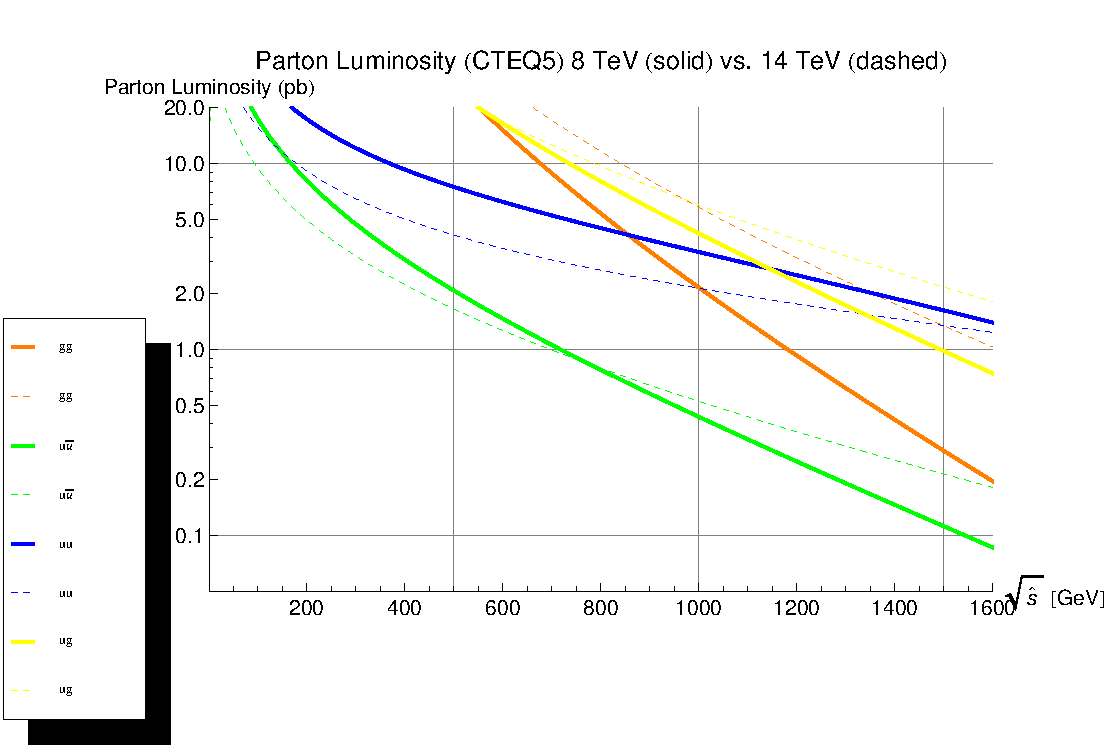
\includegraphics[width=.95\textwidth]{pics/parton_lumi_8TeV_14TeV}
\end{center}
\caption{Contours of the parton luminosity function derived from CTEQ5 parton distribution functions for $\sqrt{s}=8$ TeV and
$\sqrt{s}=14$ TeV. Contours are separated by collions the individual partons in the collision.  }
\label{fig:deltaRcones}
\end{figure}

Here the center term is refered to as the parton luminosity function and contains the parton distribution functions with
some extra accounting for the parton types to avoid double counting:
\begin{align*}
\tau\frac{dL_{ij}}{d\tau} = \frac{1}{1+\delta_{ij}} \int_0^1 dx_1 dx_2 \times \left [ (x_1 f_i(x_1,\mu^2) x_2 f_j(x_2,\mu^2)) + (1 \leftrightarrow 2)) \right ] \delta(\tau - x_1x_2) 
\end{align*}

\section{Kinematic Conventions for Collider Physics} 

In experimental particle physics, due to cylindrical symmetry of our detectors it is preferrable to make a change
from a cartesian energy and momentum parmaterization to  rotationally-symmetric parameteriztion about
the collision access. Furthermore, since the center of mass frame between the two colliding particles is generally moving
relative to the lab frame, we would like parameterization of our problem which is invariant under longitudinal boosts. First, 
we will motivate using hyperbolic functions of rapidity to parameterize energy and momentum. Lets recall define the hyperbolic
trigonometric functions:
\begin{align*}
\cosh(x) &= \frac{e^{x} + e^{-x}}{2} \texttt{ , } \sinh = \frac{e^{x} - e^{-x}}{2} \text{, and }\tanh^{-1}x = \ln \left( \sqrt{\frac{1+x}{1-x}} \right)
\end{align*}
combining cosh and arctanh conveniently gives the relativistic $\gamma$ factor for $x=\beta$:
\begin{align*}
\cosh{(\tanh^{-1}{x})} &= \frac{1}{2} \left ( \sqrt{\frac{1+x}{1-x}} + \sqrt{\frac{1-x}{1+x}} \right ) = \frac{1}{2} \left( \frac{(1+x) + (1 -x)}{\sqrt{1-x^2}} \right)  = \frac{1}{\sqrt{1-x^2}}
\end{align*}
and similarlly dervied:
\begin{align*}
\sinh{(\tanh^{-1}{x})} = \frac{x}{\sqrt{1-x^2}} = x \gamma(x)
\end{align*}
If we define $w = \tanh^{-1}(\beta)$ we can conveniently write the energy and mommentum as:
\begin{align*}
E &= \gamma m = m \cosh{w} \\
|p| &= \gamma m \beta  = m \sinh{w} 
\end{align*}
Now lets re-write a lorrentz boost $\gamma$ along the z-axis in terms of $w$:
\begin{equation} \label{eq:boost}
E' = \gamma (E - \beta p_z)   = E \cosh w - p_z \sinh w\\
p_z' = \gamma (p_z - \beta E) = p_z \cosh - E \sinh w
\end{equation}
We now set $w = y = \tanh^{-1}(\beta_z^*)$ where $\beta_z^*$ is the boost required to reach the frame where the particle is
moving only transversely to the beamline $p_\mu^*$. We can then reach the lab frame by performing
 the transformation from the $*$ frame. First lets write the four vector in the $*$ frame
\begin{align*}
 p_\mu^* &= ( E , p_x, p_y, 0 ) = (\sqrt{p_T^2 + m^2}, p_T\sin \phi, p_T \cos \phi, 0)\\
\rightarrow  p_\mu^{lab} &= (m_T \cosh y, p_T \sin \phi, p_T \cos \phi, m_T \sinh y)
\end{align*}
where $m_T = \sqrt{m^2 + p_T^2}$, $p_T = \sqrt{ p_x^2 + p_y^2}$, and $y$ is the definition of rapidity generally used in particle
physics. In the limit of light masses relative to the  transverse energy of a collision, as is generally
 the case for collisions at the Large Hadron Collider:
\begin{align*}
p^\mu = p_T(\cosh \eta , \sin \phi, \cos \phi, \sinh \eta)
\end{align*}
From the experimental perspective, what is most important about this definition is that there is a simple geometric relation
between pseudorapditiy and the angle of the particle relative to the beam line. To see this, we go back to the definition
of rapidity and take $\beta\rightarrow 1$ or equivalently $|p|=E$:
\begin{align*}
y = \tanh^{-1} ( \beta_z^* ) = \ln \left ( \sqrt{\frac{1+\beta_z^*}{1-\beta_z^*}  }\right ) \approx^{\beta\rightarrow\infty} \ln \left ( \sqrt{\frac{1+p_z/|p|}{1-p_z/|p|}  }\right )
\end{align*}
Now if we consider the angle with the beamline in the lab frame $\theta$ we use a half angle trigonometric identity.
\begin{align*}
1+ \cos \theta = 1 +\frac{p_z}{|p|} = 2 \cos^2 (\theta / 2) \\ 
1- \cos \theta = 1 -\frac{p_z}{|p|} = 2 \sin^2 (\theta / 2)
\end{align*}
combining this with the approximation with massless limit of $y$ we obtain pseudorapidity $\eta$:
\begin{align*}
\eta = \ln \left ( \sqrt{\frac{\cos^2{(\theta/2})}{\sin^{2}{(\theta/2)} }}  \right) = - \ln \left ( \tan \frac{\theta}{2} \right )
\end{align*}
\begin{figure}
\begin{center}
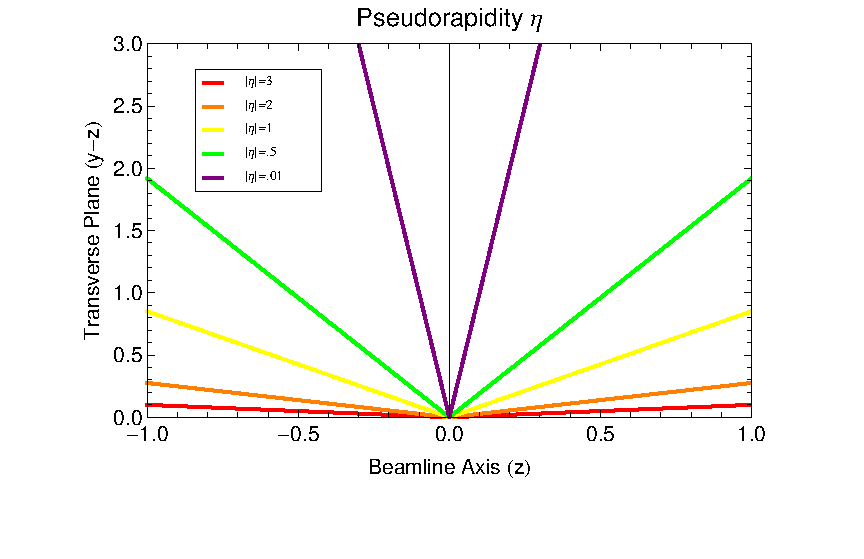
\includegraphics[width=.6\textwidth]{figures/exp_proj/pseudorapidity}
\end{center}
\caption{Lines of constant pseudorapidity in the z-y plane}
\label{fig:pseudorapidity}
\end{figure}
The energies of particles at the LHC are typically negligible in  mass relative to their energies and the approximation $\eta \approx y$ is accurate. This
 has a number of useful applications. Firstly, differences in rapidity are invariant 
under longitudinal lorrentz boosts along the beam axis which can be seen by applying the transformation in terms of $\gamma$ factors to $y_1 - y_2$  as found in Equation \ref{eq:boost}. Given this relation, pseudorapidity provides an intuitive geometric interpretation as the angle from the beam axis. The ray extending directly transverse from the collision point is $\eta=0$ with symmetric values $\pm|\eta|$ to either side of this ray along the z-axis Figure \ref{fig:pseudorapidity}. 
\begin{align*}
\Delta R = \sqrt{ (\Delta \phi)^2 + (\Delta \eta)^2}
\end{align*}
Fixed values of $\Delta R$ form a solid angle ``cone'' extending from the interaction point outward. This can be seen by
 using our definition of $\eta$ to convert from cylindrical coordinates to $(x,y,z)$ and consider the distance relative to the point $(\eta_0,\phi_0)$
\begin{align*}
\Delta R = \sqrt{ \left( \phi_0 - \tan^{-1} (y/x) \right )^2 + \left ( \eta_0 + \log \left( \tan \frac{\cos^{-1} (z/\sqrt{x^2+y^2})}{2} \right) \right)^2 }
\end{align*}

\begin{figure}
\begin{center}
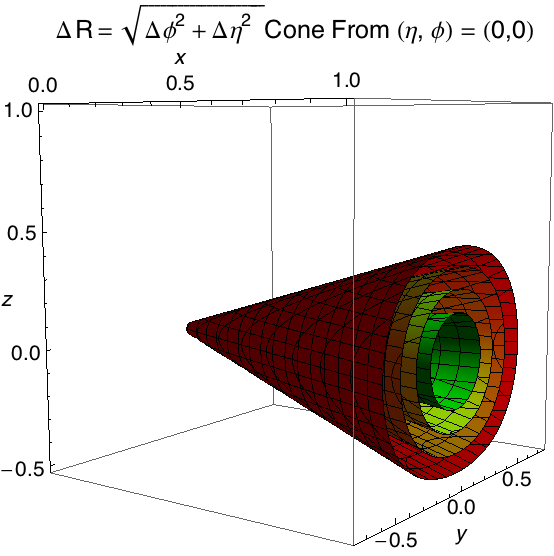
\includegraphics[width=.3\textwidth]{figures/exp_proj/deltaR_cone}
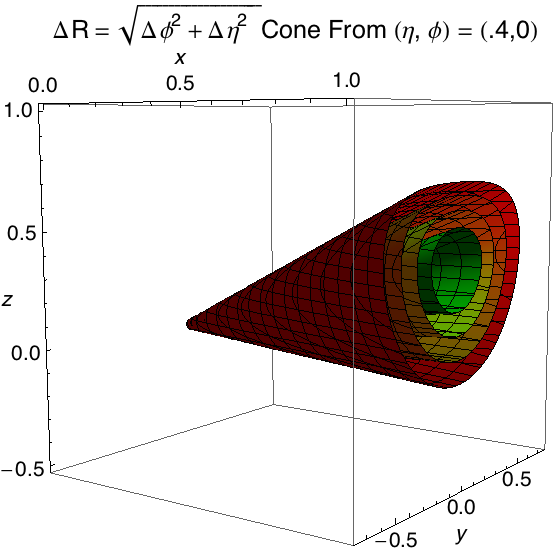
\includegraphics[width=.3\textwidth]{figures/exp_proj/deltaR_cone_eta0p4}
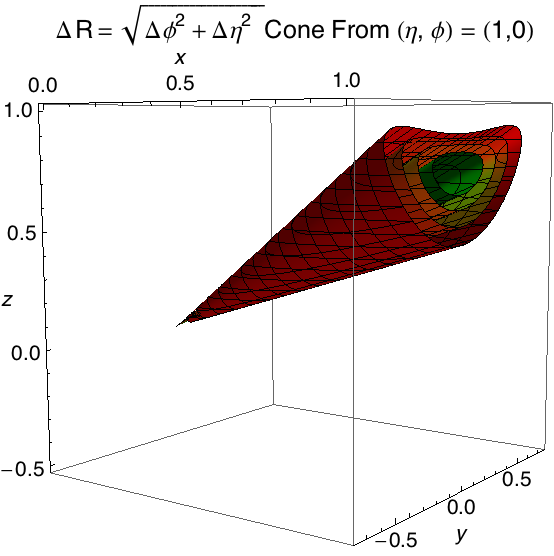
\includegraphics[width=.3\textwidth]{figures/exp_proj/deltaR_cone_eta1p0}
\end{center}
\caption{Contours of constant $\Delta R$ from the $\eta_),\phi_0 = 0,0$}
\label{fig:deltaRcones}
\end{figure}

\section{Showering}

\begin{figure}
\begin{center}
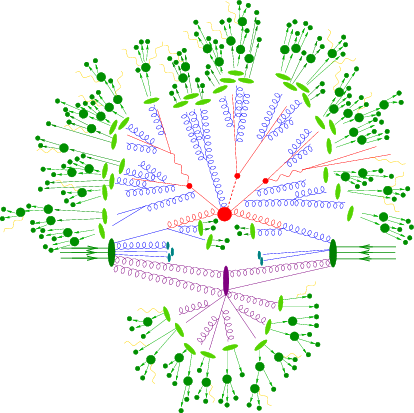
\includegraphics[width=.45\textwidth]{pics/hadronization}
\end{center}
\caption{A graphic depiction of the showering and hadronization process. The incoming protons can be see as the two sets of three
incoming arrows represting the proton quark content.}
\label{fig:showering}
\end{figure}


After the intial hard process is simulated, even if performed at high orders in perturbation theory, we have not described the large multiplicity and variety of particles which result from the showering of free quarks (Fig.~\ref{fig:showering}). We 
might even take for granted (as experimentalistics that is) that high energy proton 
collisions yield collimated showers of hadrons we more commonly refer to as \textit{jets}. 

As the collisions are made between hadrons, the dominant fraction
of the total cross section is governed by the dynamics of QCD. The strength of QCD is set by the strong coupling $\alpha_S(q^2)$ where the $q^2$ dependence arises from loop corrections to the tree level feynman diagram vertices (cite-tully). 
\begin{equation} \label{eq:running_qcd}
\alpha_s(q^2) = \frac{12\pi}{(33-2n_f)\ln{(q^2 /\Lambda_{QCD}^2})}
\end{equation}
Here $n_f$ is the number of flavors of participating fermions in the interaction and $\Lambda_{QCD}=0.1-0.3$. Here we notice two important features. As $q^2$ becomes large, the interaction because asymptotically weak and the physics is perturbative. As $q^2\rightarrow \Lambda_{QCD}$ the theory is
strongly coupled ($\alpha > 1$) and a perturbative approach leaves higher order terms that cannot be neglected 
(cite-ellis-qcd). 

We need a method to evolve the high energy states to some low energy cut off where the physics is clearly non-preturbative. 
This scale is typically taken to be on the order of momentum transfer $t^2 = 1$ GeV$^2$.
This consistutes a natural division of labor for generating physics events between the perturbabtive hard scattering, the approximately perturbative showering, and the non-preturbative physics of hadronization. The terms fragmentation and hadronization are often used interchageably to describe the non-preturbative of this divison. However, in certain contexts, hadronization can refer to the both the parton showering as well as hadron formation. 

In experimental high energy particle physics the term Monte Carlo (MC) is used as a short hand for simulated 
physics samples, however the Monte Carlo method of generating
these samples means something specific. Monte Carlo methods generally rely on using random numbers to simulate 

%% A Monte Carlo algorithm sacrifices the accuracy of the result for a time complexity speed up.
%% This is to be contrasted with a Las Vegas algorithm, which always returns correct results, but the run time is probalistic (and 
%% finite). 
 
(cite-ellis-qcd) The monte carlo method of generating parton branching is stated as: given some 
virtual mass scale $t_1$ and momentum fraction $x_1$ generate
 $(t_2, x_2)$ after one step in the branching evolution. To perform this step-wise evolution of the parton 
branching we need shower evolution equations.

(cite-mrenna-showering) Consider the branching of a particle $a$:  $a\rightarrow bc$ with a 
momentum scale $Q^2$. We denote energy and momentum fraction imparted to particle $b$ as $z$
 such that particle $c$ receives $1-z$. We introduce the momentum
transfer variable motivated by Equation \ref{eq:running_qcd} $t = \ln (Q^2 / \Lambda^2)$ yielding 
a differential element $dt = d\ln (Q^2) = dQ^2/Q^2$. The
differential probability for the particle $a$ to branch is given:
\begin{align*}
d\mathcal{P} = \sum_{b,c} \frac{\alpha_{abc}}{2\pi} P_{a \rightarrow bc}(z) dt dz 
\end{align*}
where the sum is over all possible branchings and $\alpha$ is the appropriate 
coupling $(\alpha_{EM},\alpha_{S})$  for the branching evaluated at the appropriate scale. We enumerate the kernels that map the momentum fraction from splitting
 to the possible states after branching:
\begin{align*}
P_{q\rightarrow qg} (z) &= C_F\frac{1+z^2}{1-z}   &P_{q\rightarrow q\gamma} (z) &= e_q^2\frac{1+z^2}{1-z}\\
P_{g\rightarrow gg} (z) &= N_C\frac{(1-z(1-z))^2}{z(1-z)} &P_{l\rightarrow l\gamma} (z) &= e_l^2\frac{1+z^2}{1-z} \\ 
P_{g\rightarrow q\bar{q}} (z) &= T_R (z^2 + (1-z)^2)\\
\end{align*}
where $C_F=4/3$ is a color factor, $N_C$ is the number of colors in QCD, $T_R = n_f / 2$ is half the number 
of allowed $q\bar{q}$ flavors. $e_i^2$ is the charge squared of the quark or lepton. 

Lets define an integral over the probability distribution for some fixed $t$ between the
minimally allowable momentum fraction $z_{-}$ and the maximum $z_{+}$ as:
\begin{align*}
\mathcal{I}_{a \rightarrow bc} (t) = \int_{z_{-}(t)}^{z_{+}(t)} dz \frac{\alpha_{abc}}{2\pi} P_{a\rightarrow bc} (z) 
\end{align*}
From this here we can find the total probability of branching as a sum over the
possible branching states $p_{branch} = \sum_{bc} \mathcal{I}_{bc}(t)$. If we consider the probabiity of no branching occuring $(1-p_{branch})$ in some finite
interval $(t,t_0)$ as the product of differential time steps $\delta t$, we obtain an exponential:
\begin{align*}
\mathcal{P}_{no-branch}(t_0,t) = \prod_{\delta t \in (t,t_0)} (1-p_{\text{branch}}) &\approx \lim_{N\rightarrow \infty} 
\sum_{k=0}^{N} \frac{N!}{(N-k)!k!} 1^{N-k}(-p_{\text{branch}})^k  \\
&= \sum_{k=0}^{\infty} \frac{1}{k!} (-p_{branch})^k = \exp{(-p_{branch})}
\end{align*}
Such that the total probability of not branching within a givern $t$ interval is given:
\begin{align*}
\mathcal{P}_{no-branch}(t_0,t) = 
\exp { \left ( - \int_{t_0}^{t} dt' \sum_{b,c} \mathcal{I}_{a\rightarrow bc} (t')   \right )} = S_{a}(t)
\end{align*}
Where we have introduced the notation $S_a(t)$ for what is referred to as the Sudoakov form 
factor (cite-sudakov). With this single parameterization we can write the probability of not branching as a ratio of $S_a(t)$ functions (since the ratio of exponentials will just alter the integral bounds):
\begin{align*}
\mathcal{P}(t_2, t_1) = \frac{S_a(t_{2})}{S_a(t_1)}
\end{align*}
Note here that $t$ is not time, but rather serves a proxy for time, where the
final state showering occurs from an intial $t_{max}$ set by the hard scattering and progressively becomes smaller through the branching process.   

The Monte Carlo process generates a random number $\mathcal{P}$ and solves for $t_2$ in terms
of $t_1$. The process is then applied to the newly branched particles $b$ and $c$. If $t_2$ is smaller than the scale
 set for hadronization, then the showering process terminates. Eventually from the monotonicity of $t_i$ the cascade
terminates and the generation process is handed off to hadronization.

\section{Hadronization} 

When the quark model, the eight-fold way, was orignally introduced in 1961, it was a large simplification of the space of observed  particles. Each combination of possible light quarks was observed in nature (the third generation had not 
yet been discovered). However, a  single ``bare'' quark had never been observed despite experimental efforts. Today
we understand that it is the inherent nature of the strong force that prevents light quarks from being liberated from their 
hadronic bound states. The discovery of the top quark, who's width is  larger than $\Lambda_{QCD}$, 
will decay before hadronization takes place allowing for the study of a ``bare'' quark. In this section, we breifly discuss
 the way  monte carlo simulation models the non-preturbative confinement of quarks.

(cite-ellis) When we leave the showering process, we are left with a large number of virtual particles on the order of the cutoff $t_{min}$. Although this
parameter is unrelated to the hadronization process, an ideal hadronization model would use the chosen value of $t_{min}$ to compensate for
 effects of having a hard cutoff value for the showering. 
 As $t_{min}$ is increased, there are fewer particles that are increasingly off-shell. These virtual particles should be
 able to hadronize, however, the favored values of $t_{min}$ to begin the hadronization step tend to be a few times the
 scale of hadronization $\Lambda_{QCD} \approx 0.1 - 0.3$ GeV. This is suggestive that the extensions of perturbation theory
 are more reliable than models of hadronization.

(cite-mc-review) It is important to state that there are only models of hadronization and no calculations from first principles. 
Even lattice QCD calculations which are made on euclidean space times fail for processes which are inherently minkowskian 
such as hadron formation. Two main categories of hadronization models exist. The string 
model which transforms virtual particles directly into hadrons and the cluster model which uses in intermediate clustering step. 

\begin{figure}
\begin{center}
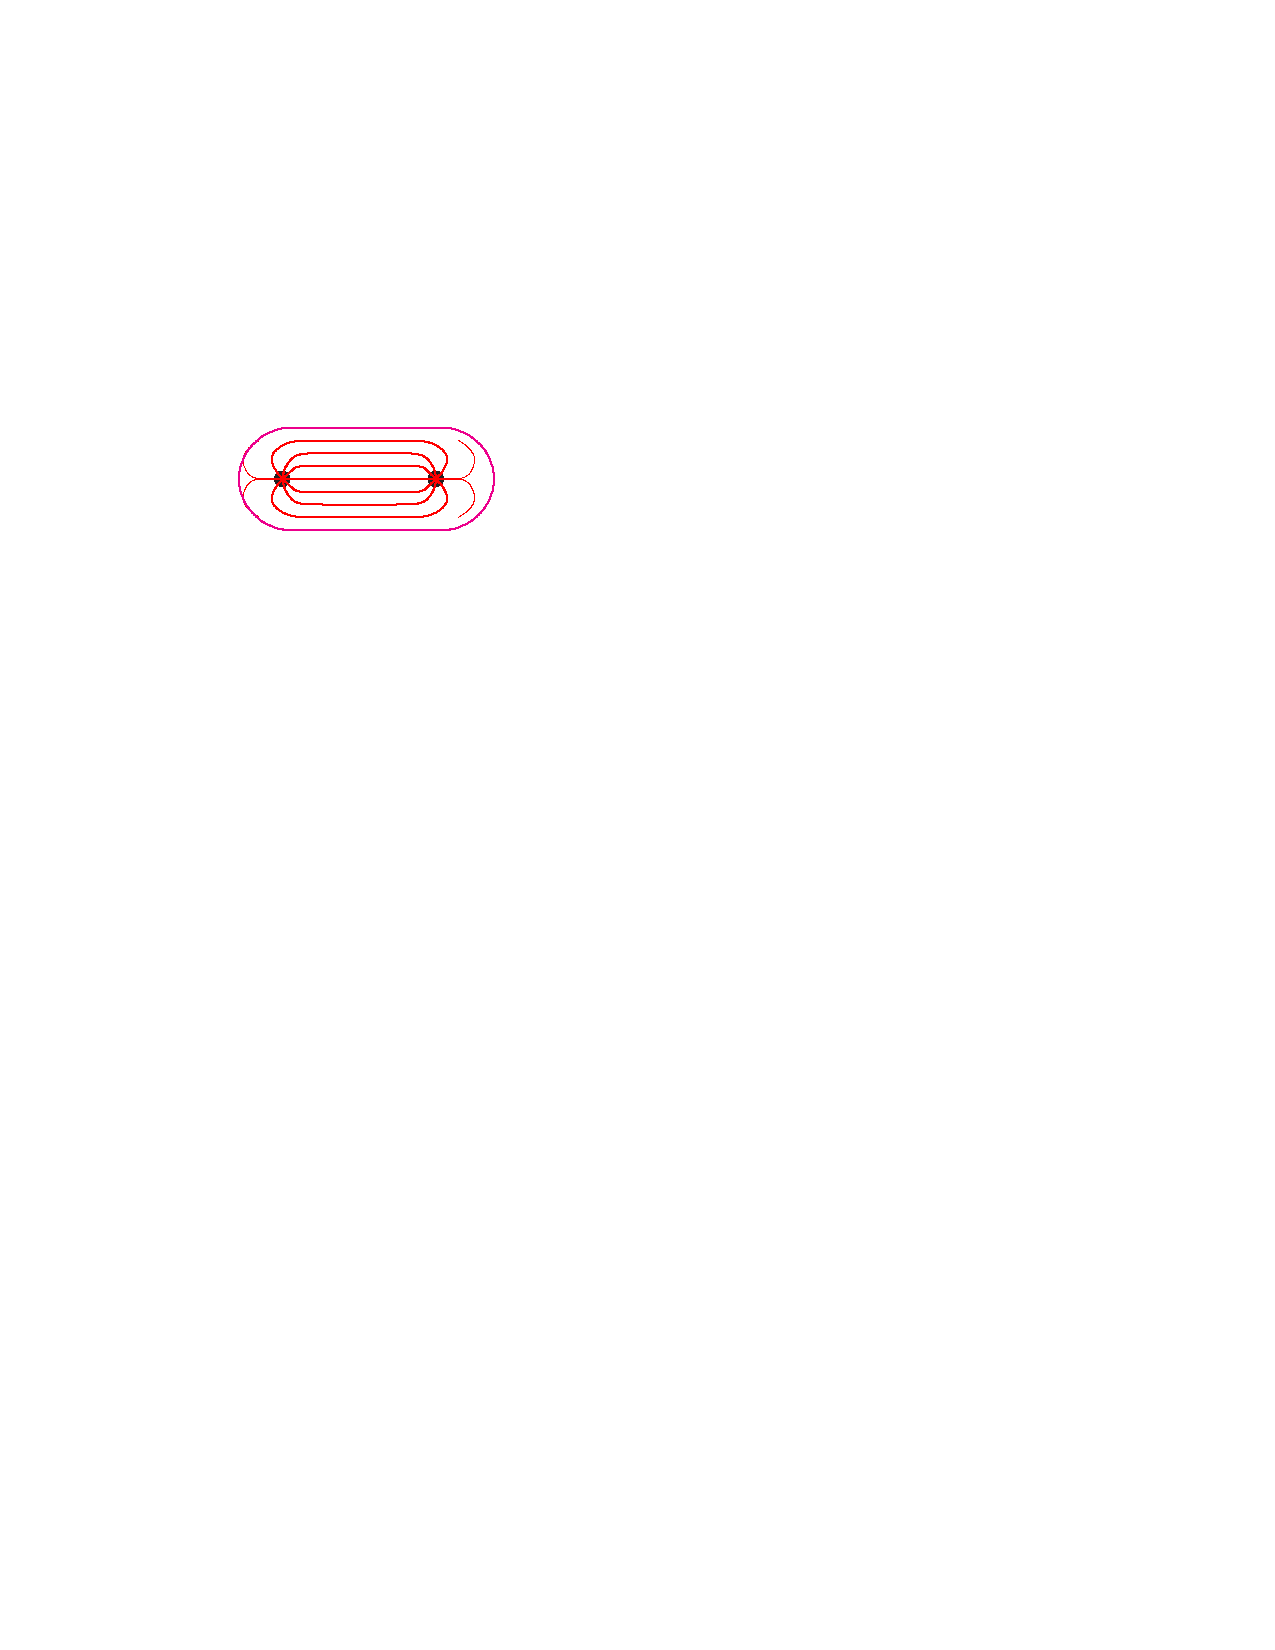
\includegraphics[width=.45\textwidth]{pics/flux_tube}
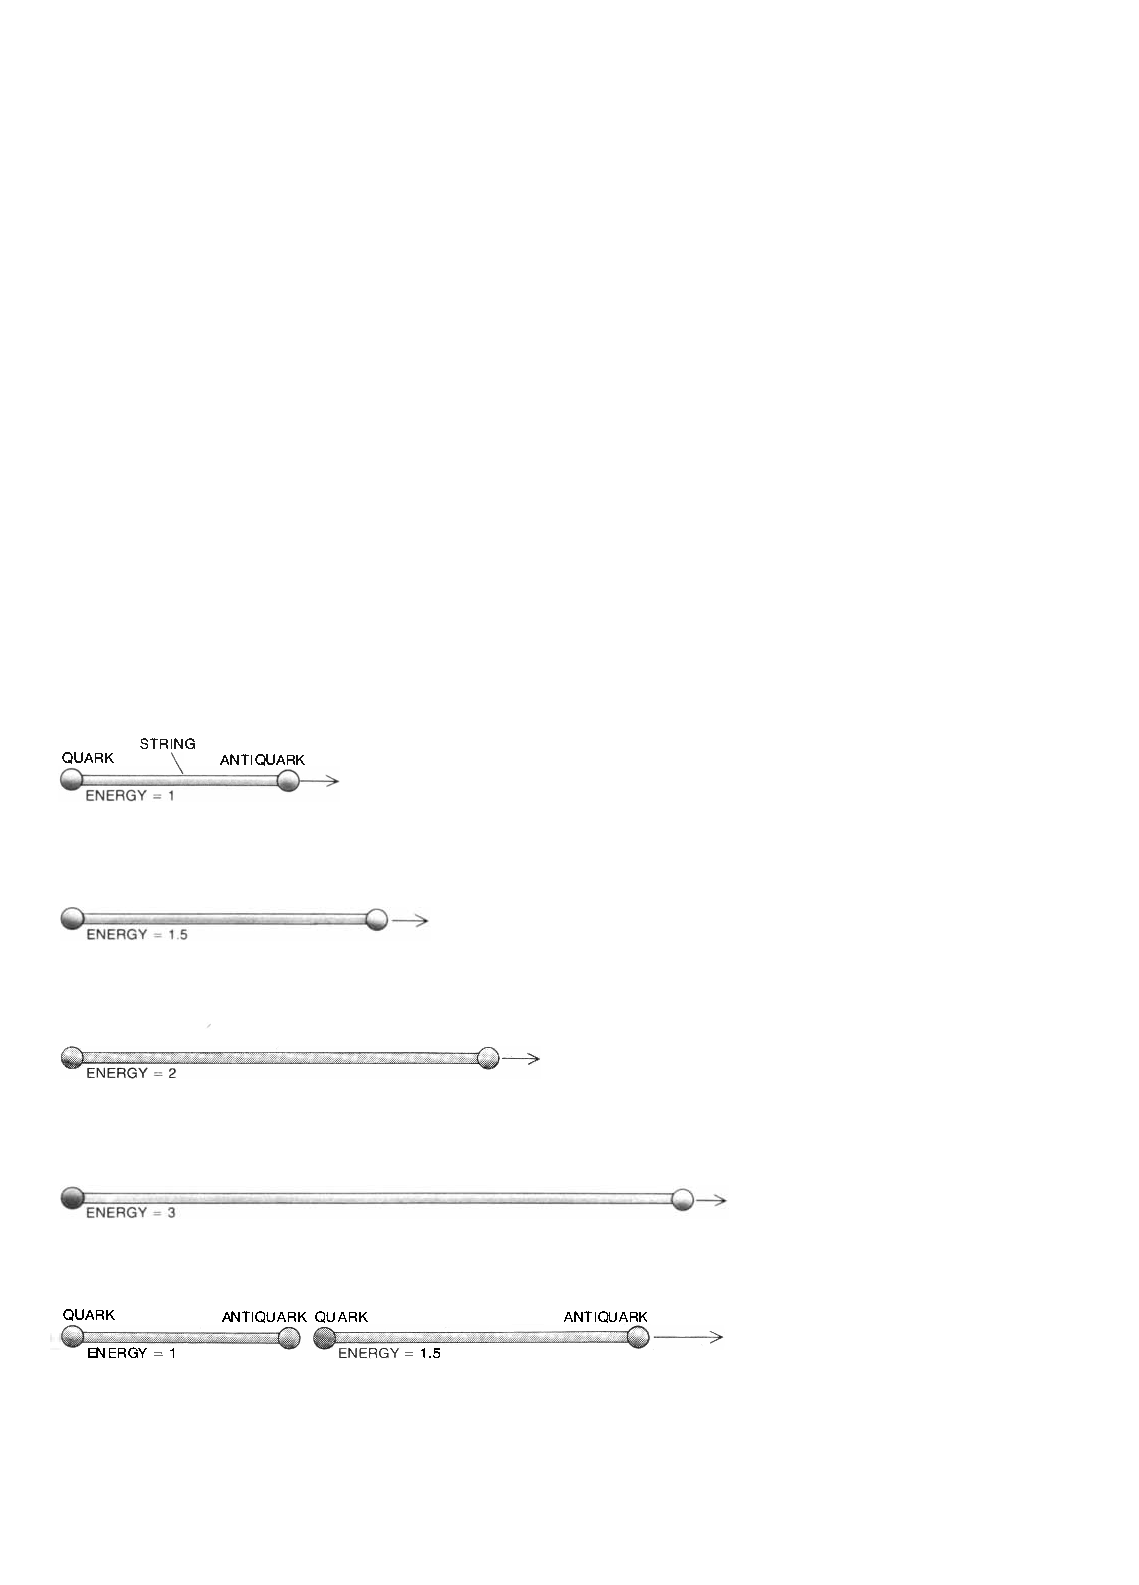
\includegraphics[width=.45\textwidth]{pics/string_stretch}
\end{center}
\caption{The flux between a quark and anti-quark (left) A simple model of quarks as the ends of a string. As an 
attempt is made to separate the two quarks, the string breaks producing two new ends i.e. quarks (right) (cite-string-sretch) }
\label{fig:flux_tube}
\end{figure}

The string model, the most well known of which is the Lund String Model (cite-lund-string), relies on an assumption of linear confinement. One expects
a linear potential $V(r) = \kappa r$ at long distances, where the string constant $\kappa \approx 1$~ GeV/fm $\approx .2$ GeV$^2$. In general, 
there is an additonial coulomb potential at shorter distances, but it is an assumption of the Lund model that this term is negligible. It is
important to note that string model of hadronization should not be confused with the strings of string theory where strings serve as the fundamental .  The linear
 confinement of QCD is best visuallized as a color flux tube being stretched between a quark and anti-quark (Figure. \ref{fig:flux_tube}). As the two
quarks are increasingly separated in space, the flux tube is stretched maintaining constant energy per unit length $\kappa$. The lorrentz covariant and
causal description of this energy flow uses a massless one dimensional string that parameterizes the axis of a cylindrically symmetric flux tube. 

\begin{figure}
\begin{center}
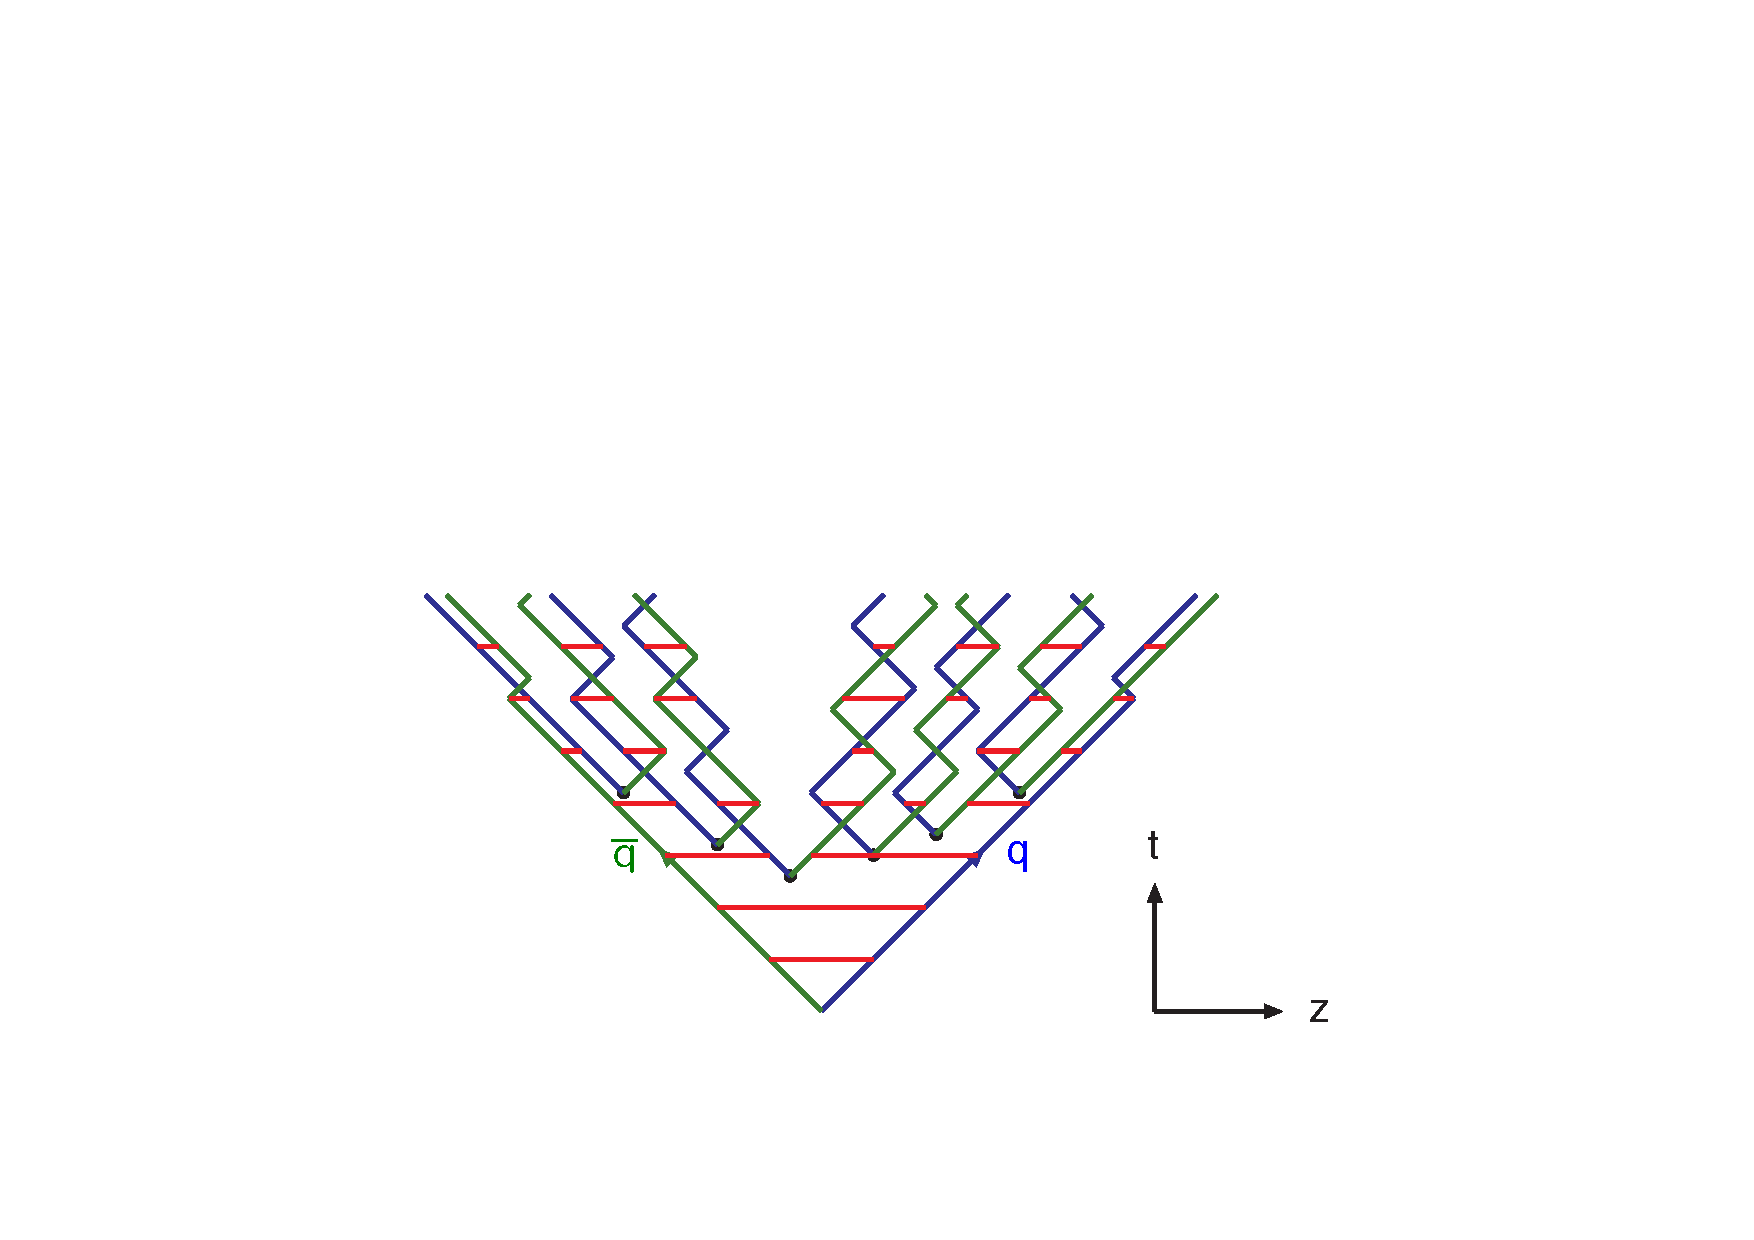
\includegraphics[width=.65\textwidth]{pics/lund_model}
\end{center}
\caption{The 1+1 dimensional propogation of the hadronization process beginning form a quark anti-quark pair.  }
\label{fig:lund}
\end{figure}


In the simple case of quark anti-quark production (Figure \ref{fig:lund), the two quarks separate from each other along the $z$ axis and the potential energy stored in the 
string increases. When the potential energy is large enough, the string can break through the production of a new quark anti-quark pair. These breaks 
typically occur between 1 and 5 fm in the rest frame of the pair, however in the lab frame these processes highly length contracted. After the break,
widening regions of no flux arise. 

The string model contains a large number of parameters related to flavor properties and must determined from data

The cluster model is based on the precontainment properties of parton showers which lead to  color singlet clusters. The cluster hadronization begins with
non-preturbative splitting of gluons into quark anti-quarks pairs. Clusters are formed from color-connected pairs. Most clusters under go two body phase-space decays, 
with heavier clusters decaying first to lighter clusters. Cluster models tend to describe the data less accurately than 
string models, but using fewer parameters.

The incredibely dense and active enviroment of hadronic collisions could lead to significant collective eeffects which are not considered in current 
hadronization models.



\section{Hadron Decay} 

\section{Jet Clustering}

\begin{figure}
\begin{center}
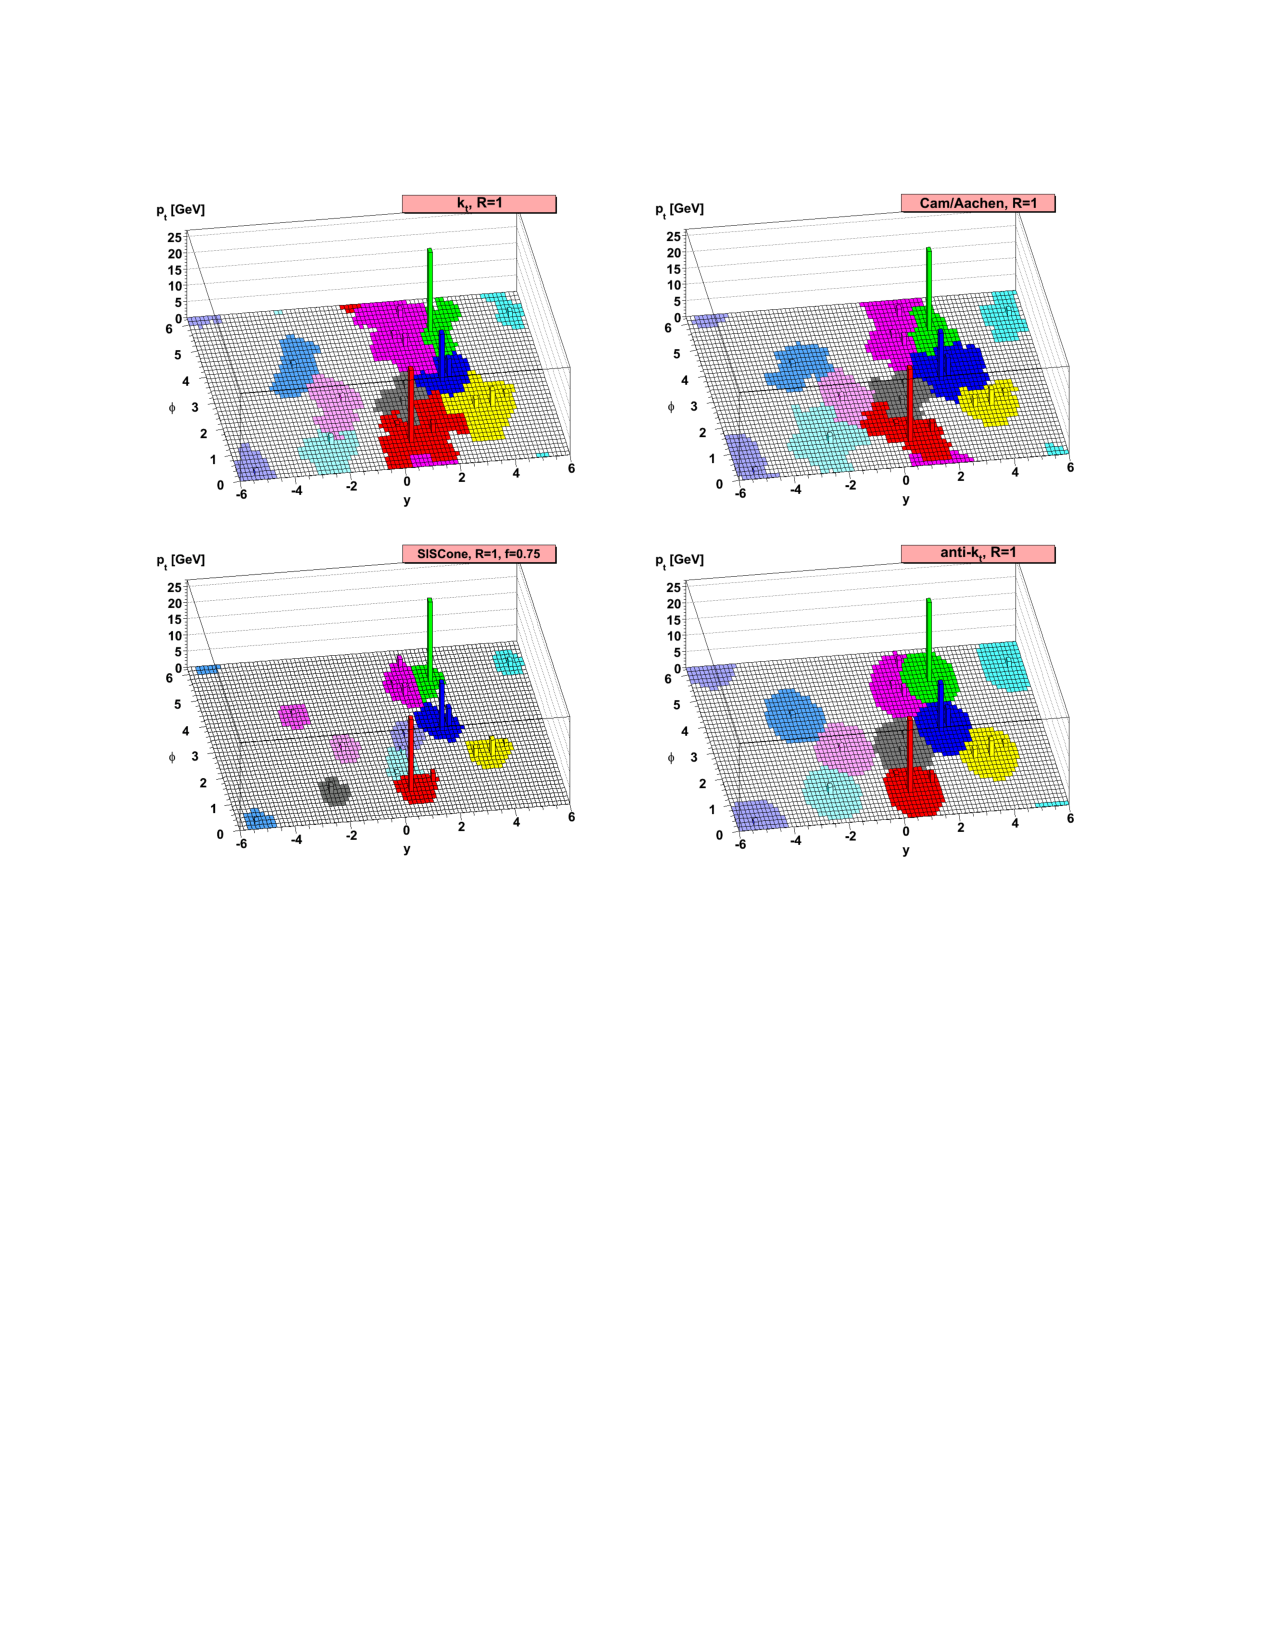
\includegraphics[width=.75\textwidth]{pics/antikt}
\end{center}
\caption{Comparisons made between varied clustering algorithms.}
\label{fig:antikt}
\end{figure}


Once the showering and hadronization have constructed the final state particles we need a way of clustering the numerous deposits or
particles in the final state simulation and data. While in simulation one can trace the
 hadrons back through their branching tree to their mother particle from the hard interaction,
data has no truth information. This problem necessitates a fast algorithm that takes as input energy deposits in the 
detector and outputs clusters with kinematic properties representative of the hard scattering process quarks and gluons. 

Any desirable clustering algorithm must satisfy collinear and infrared safety. An algorithm that is collinear safe, is insensitive to the 

The most commonly utilized clustering algorithm is anti-kt (Figure \ref{fig:antikt}) which takes a size 
parameter $R$ corresponding the $(\Delta R)^2 = (\Delta\eta)^2 + (\Delta \phi)^2$.  The resultant four momentum of
the cluster is given by the four-momentum sum of the individual deposits. 

Jets must be calibrated in data to account for energy lost. Common techniques include

Additionally as luminosity increases and there are increasingly more 
ineractions per event, jets must be corrected for additional clustered energy not related to the primary interaction. For this,
an average energy density $\rho$ is calculated event by event and $\rho\times A$ is subtracted from the jet energy where $A$ is the
jet area. 

For 2015 data, at $\sqrt{s}=13$~TeV the size parameter for the displaced jets analysis was fixed at a cone size $R=0.4$. 
Larger size parameters as well as different algorithms are utilized for boosted hadronic decays of bosons,



\chapter{Experimental Setup }

\section{Founding and History}

\section{Large Hadron Collider}

\begin{figure}
\begin{center}
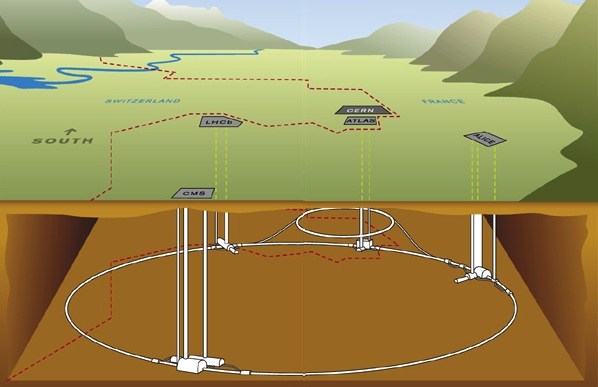
\includegraphics[width=.5\textwidth]{lhc_tunnel}
\caption{The LHC tunnel installed on the border of Geneva, Switzerland and France. 
The experiments are distributed along the circumference of the ring.}
\end{center}
\end{figure}

The bunches of protons in the LHC are bent into a circular trajectory by more than 1200
 superconducting dipole magnets and are focused and maintained close to the ideal
 orbit around the ring by hundreds of superconducting quadrupole magnets. 
Thousands of corrector magnets around the ring allow the beam to be steered closer 
to the ideal orbit, make the focusing independent of the particles’ energy variations
 within a bunch, and cancel the effects of higher order multipoles in the fields induced 
by small field imperfections in the main magnets. 
The radiofrequency (RF) field in superconducting cavities is placed periodically around 
the ring and accelerates the protons from the injection energy of 450 GeV to the final
 operating energy, which is designed to be 7 TeV per beam. The RF field also causes the
 protons to be bunched, as only particles at or near a certain ”equilibrium phase” on 
the RF wave will be accelerated stably. Special quadrupoles around each interaction region
 focus the bunches down to a small transverse size, to increase the likelihood of a
 proton-proton collision each time two bunches pass through each other.

\section{Other LHC Related Experiments}

\section{Compact Muon Solenoid Experiment}

\begin{figure}
\begin{center}
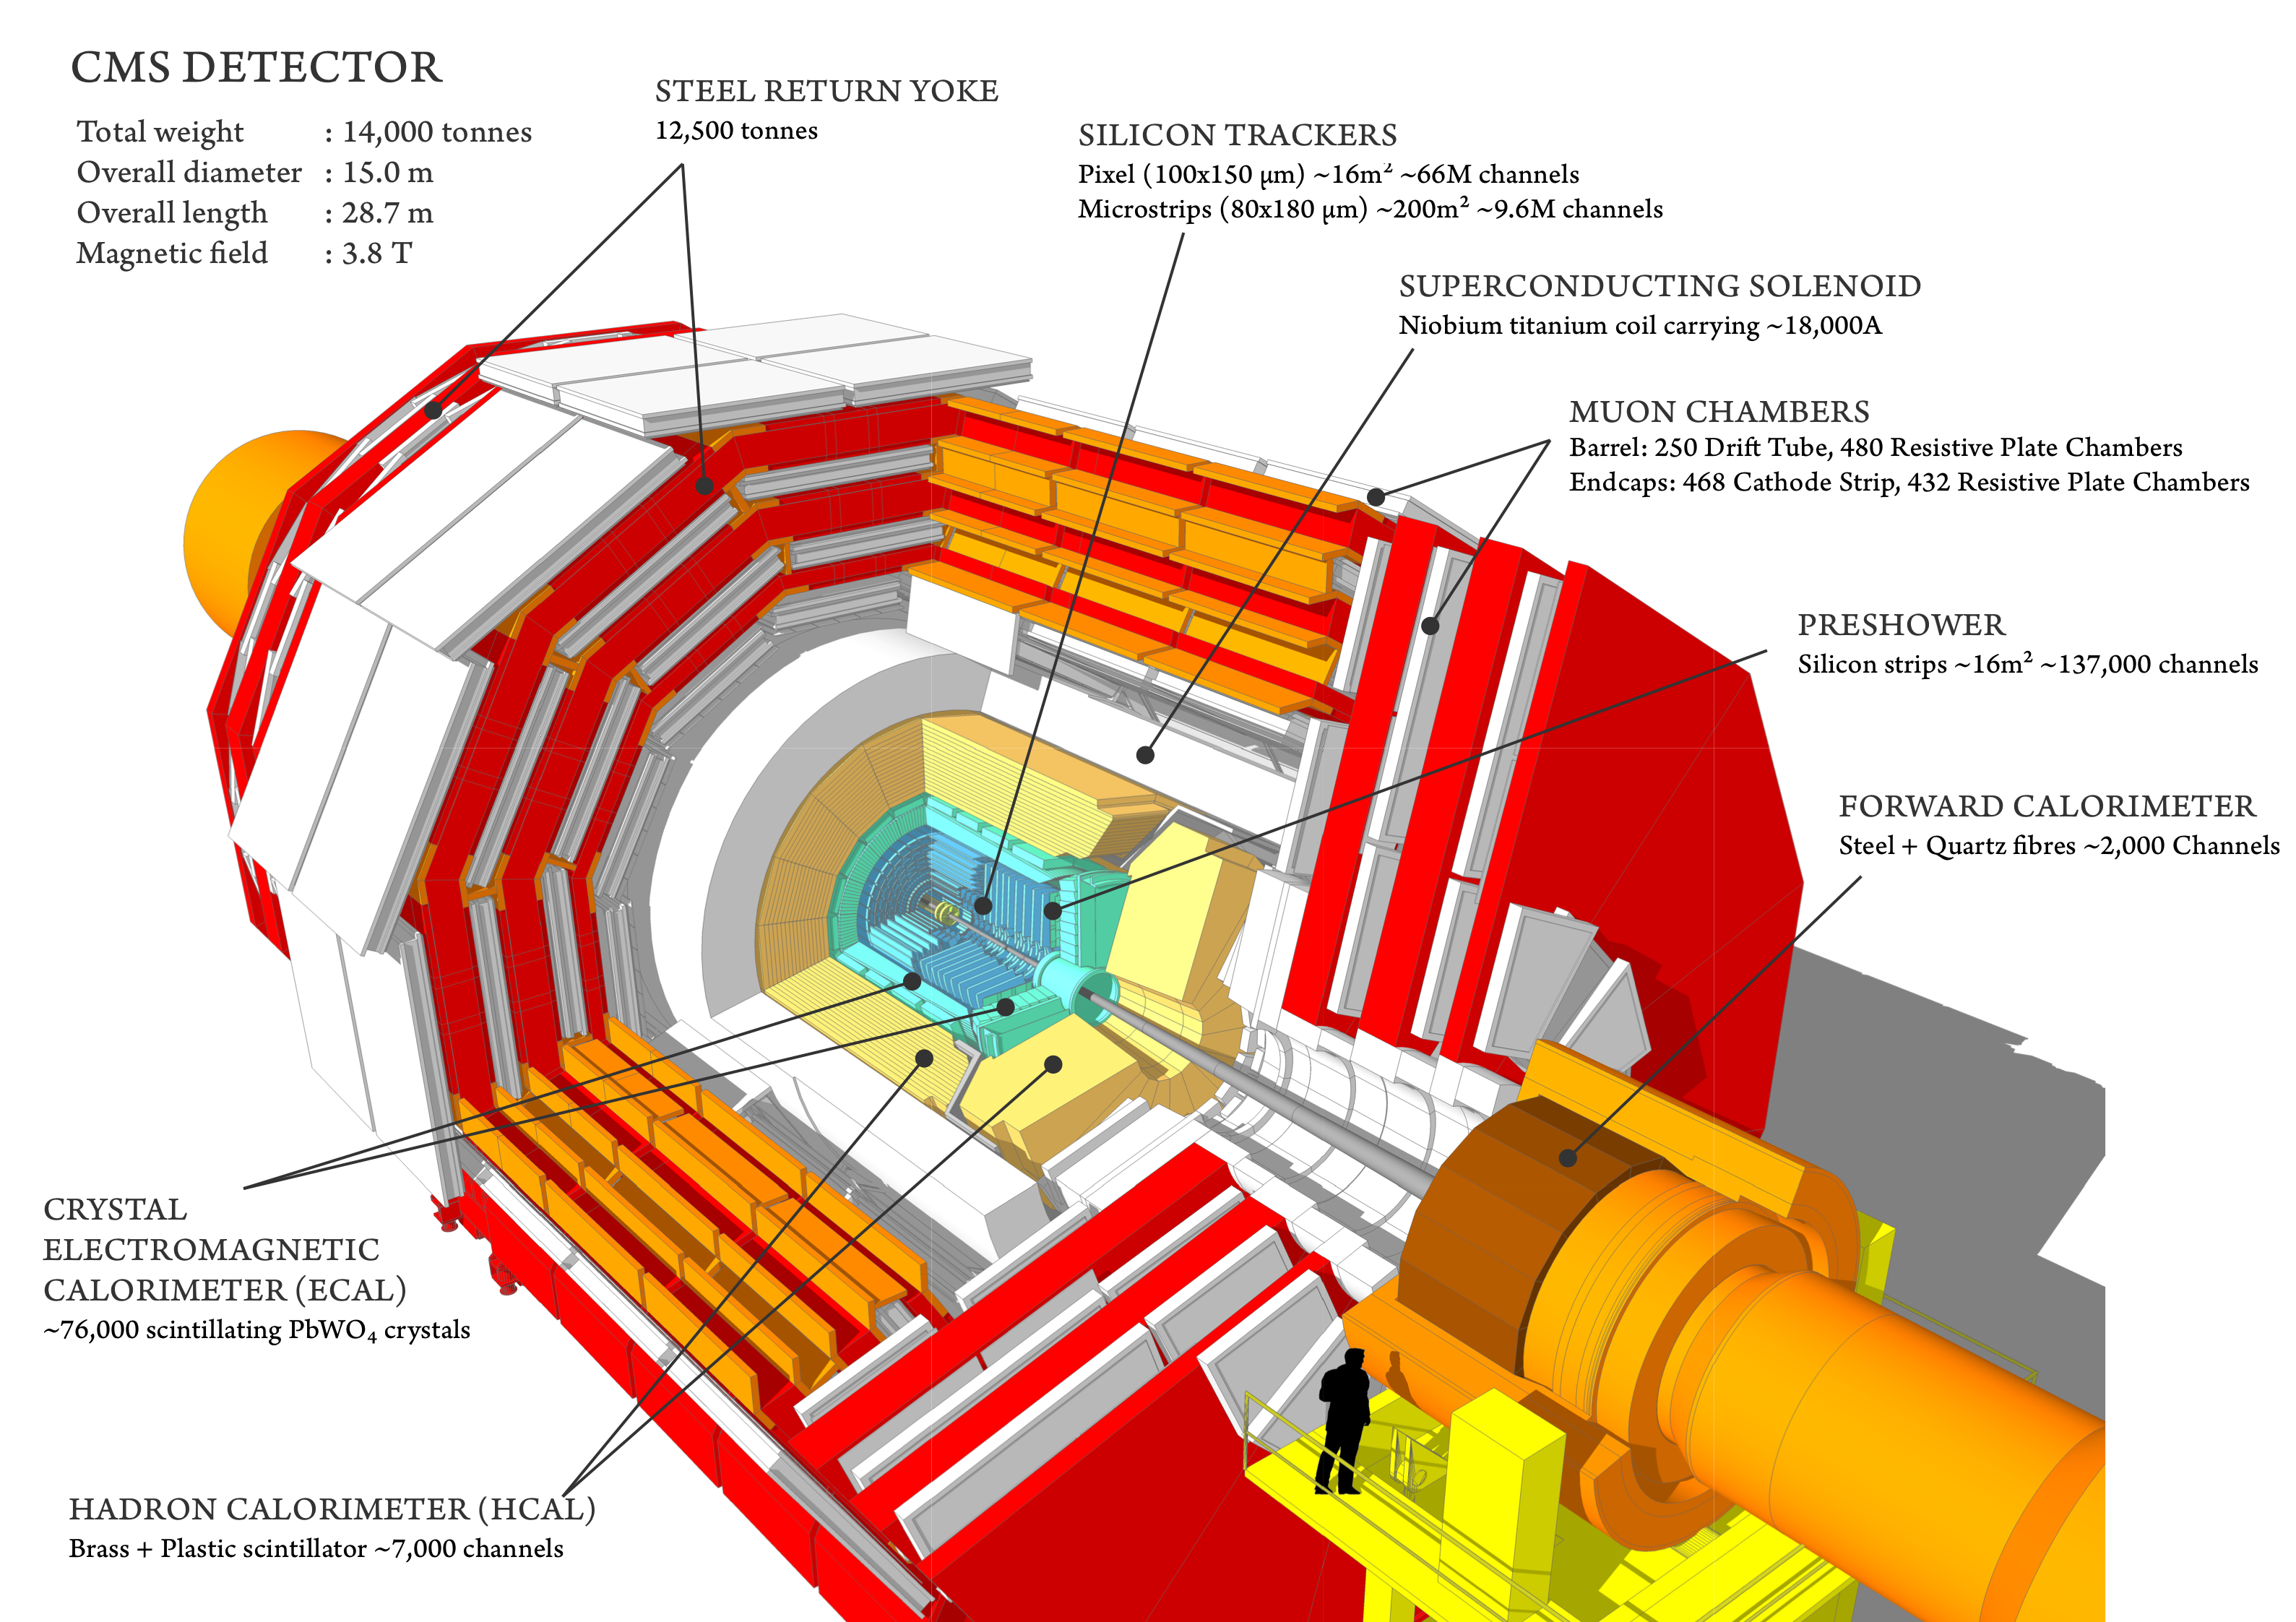
\includegraphics[width=.55\textwidth]{figures/pre_thesis/cms.png}
\hspace{.1in}
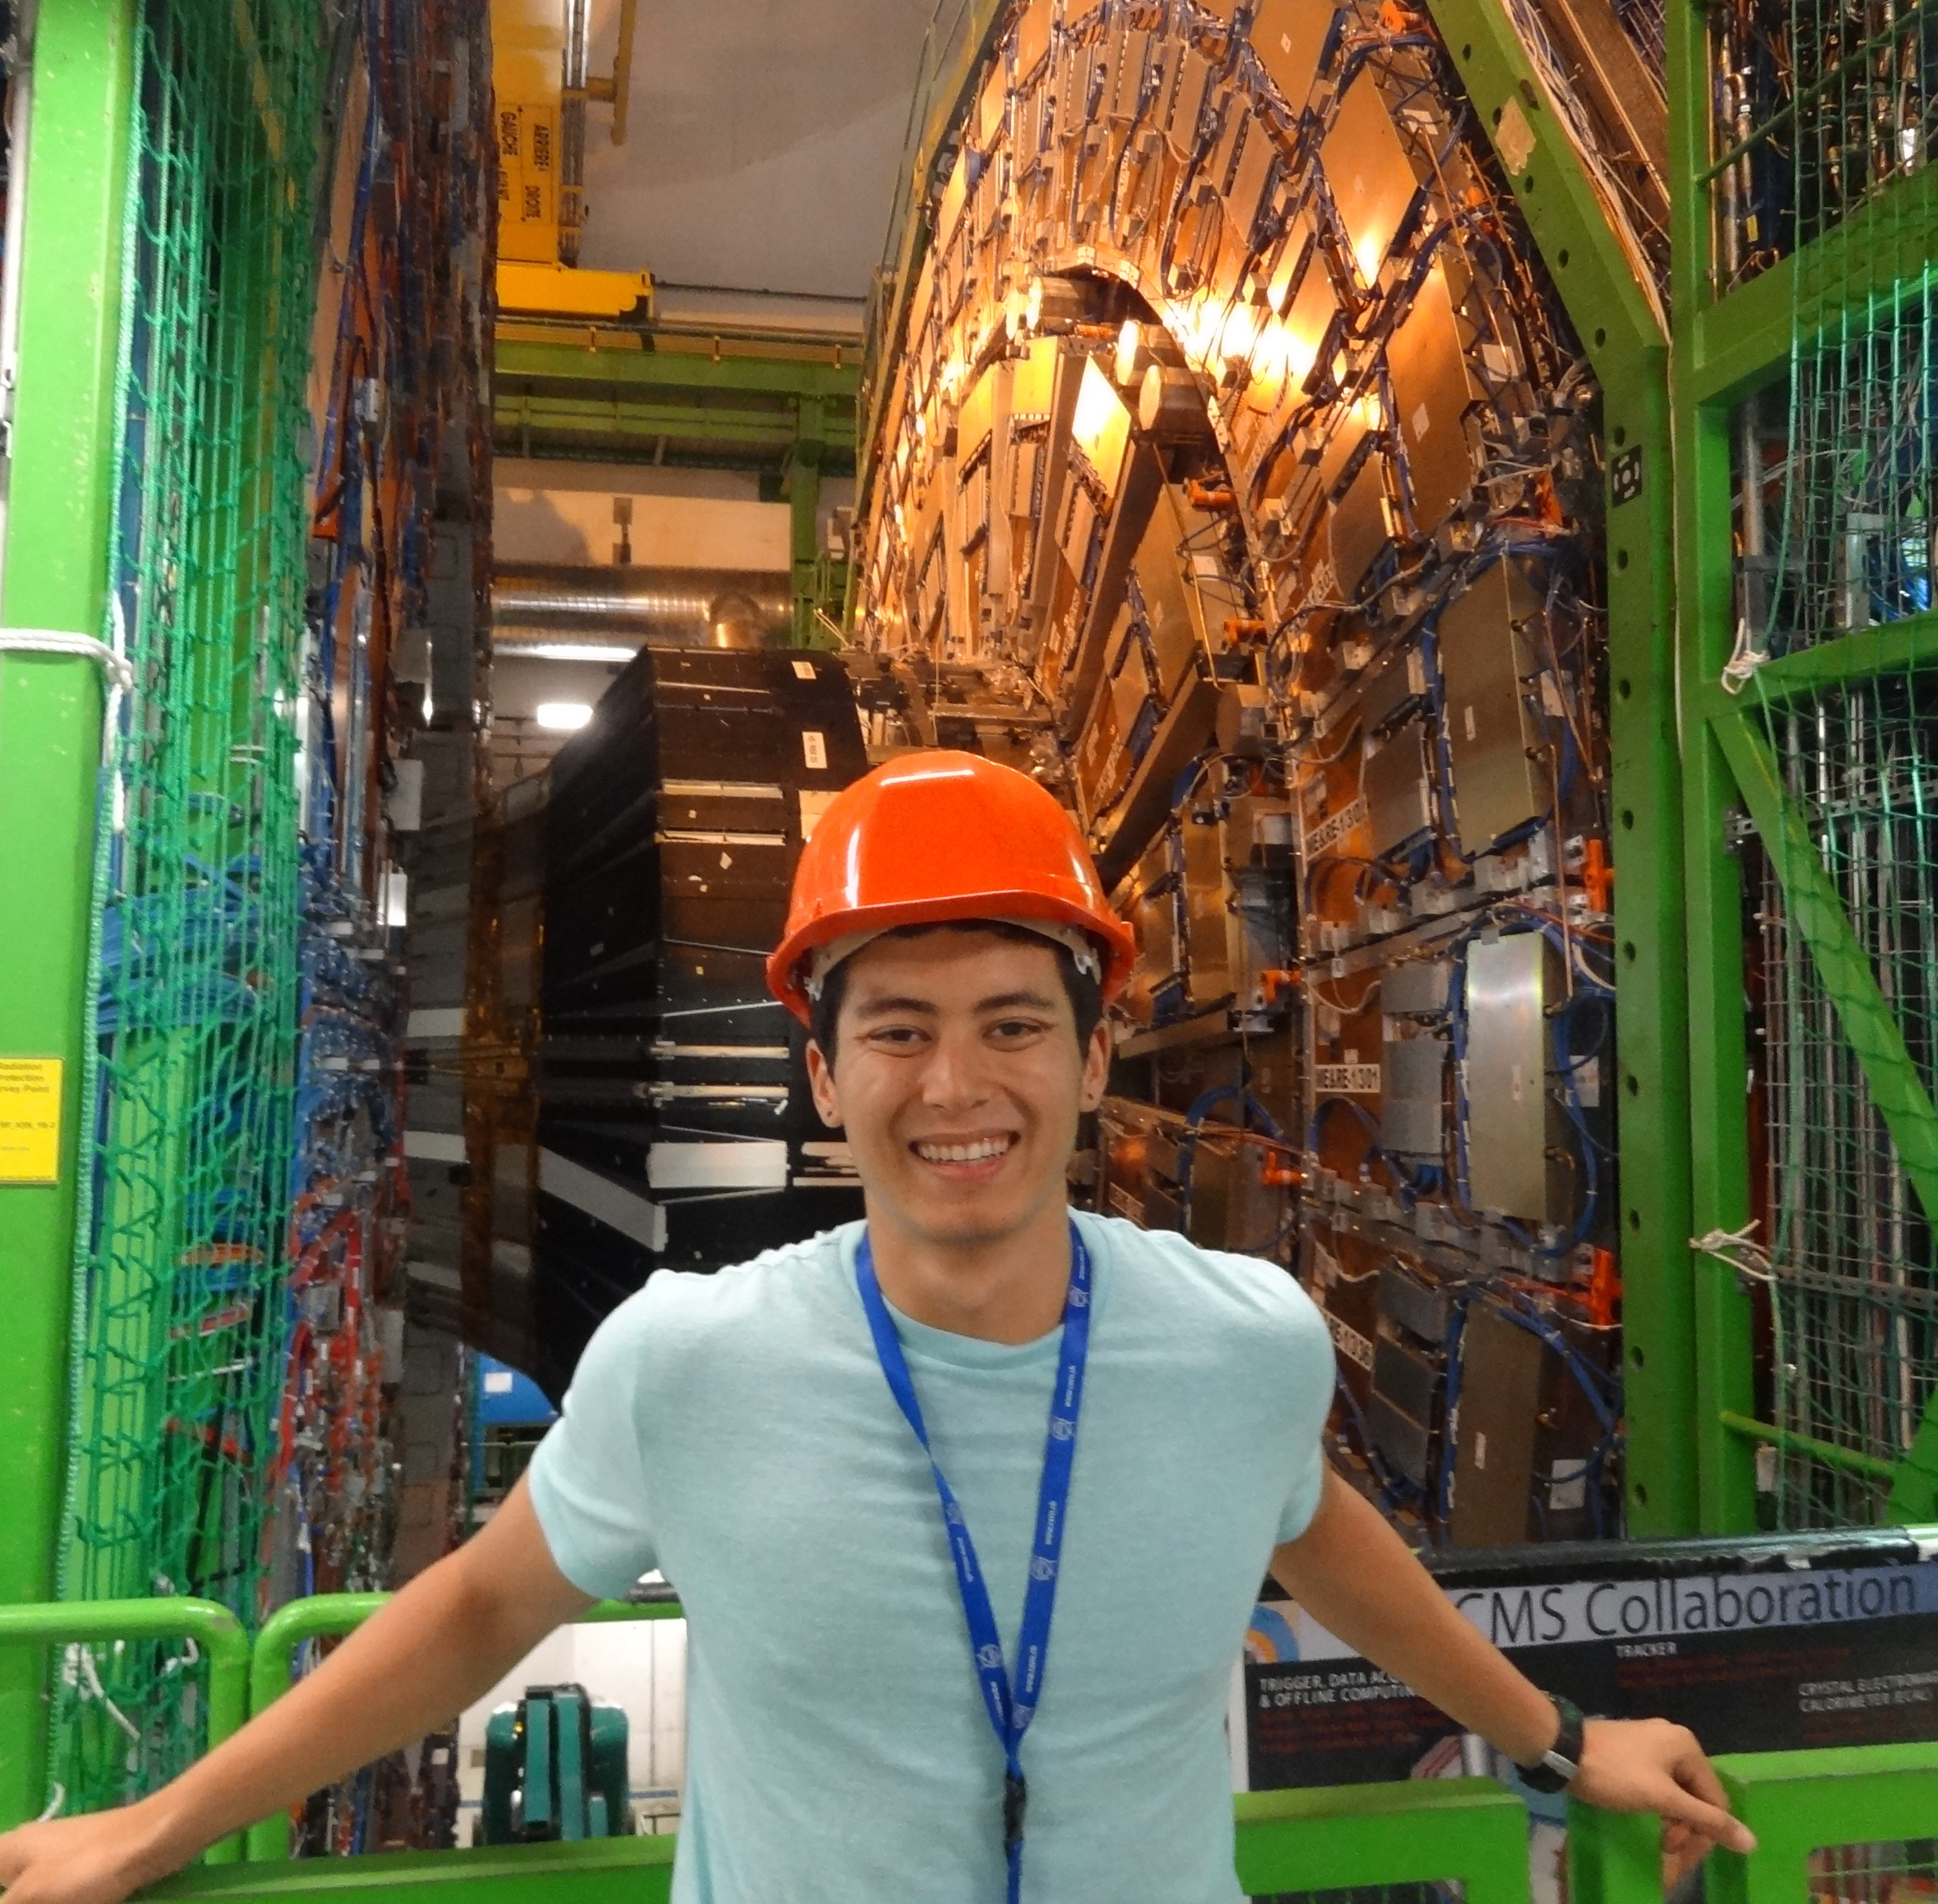
\includegraphics[width=.4\textwidth]{figures/pre_thesis/selfie}
\end{center}
\caption{(left) A tear-away view of the inner detectors of CMS. (right) The CMS endcap currently detached from the inner barrel for upgrades during the shutdown.}
\label{fig:cms}
\end{figure}

The Compact Muon Solenoid (CMS) Detector is a general-purpose detector consisting of 
an all silicon tracker, a precision electromagnetic calorimeter (ECAL), a hadron calorimeter
 (HCAL), a 4 T superconducting solenoid and muon chambers. The solenoid deflects charged
 particles whose paths are traced in the tracker, making it possible to 
reconstruct the particles’ momentum. The two calorimeters reconstruct the energy 
of and identify photons, electrons and hadronic jets.
As shown in Figure \ref{fig:cms} the detector has cylindrical symmetry about the
 interaction point where the proton beams collide. By maintaining near full coverage 
of the interaction point it is possible to detect signatures such as neutrinos or other weakly interacting particles as missing energy. 


\subsection{ECAL}

\subsection{HCAL}

\subsection{Tracking}

\begin{figure}
\begin{center}
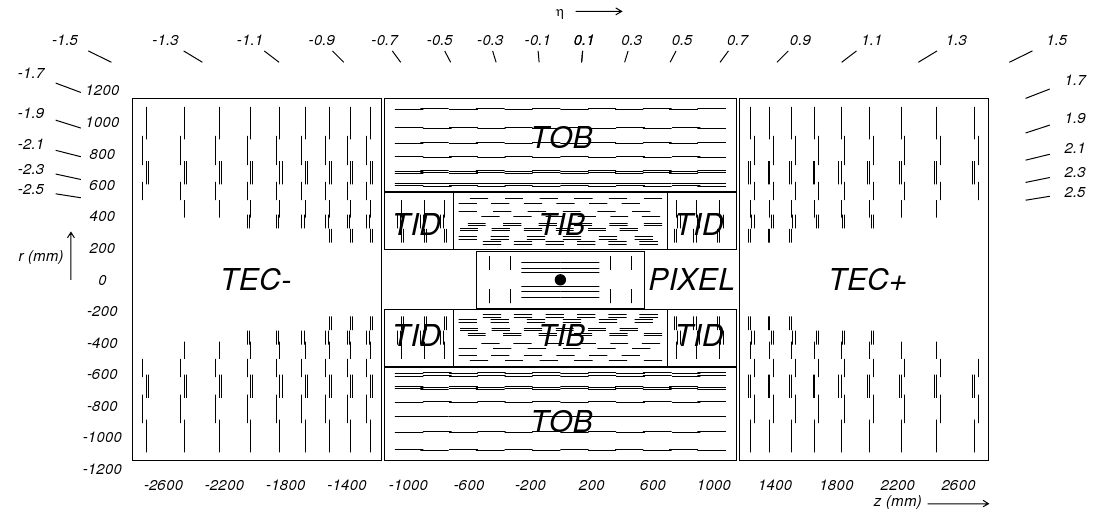
\includegraphics[width=.9\textwidth]{figures/an_jetid/DETECTOR/cms_tracker}
\end{center}
\caption{The CMS Tracker}
\label{fig:tracker}
\end{figure}

\subsection{Muon Chambers}

\subsection{Trigger System}

\begin{figure}
\begin{center}
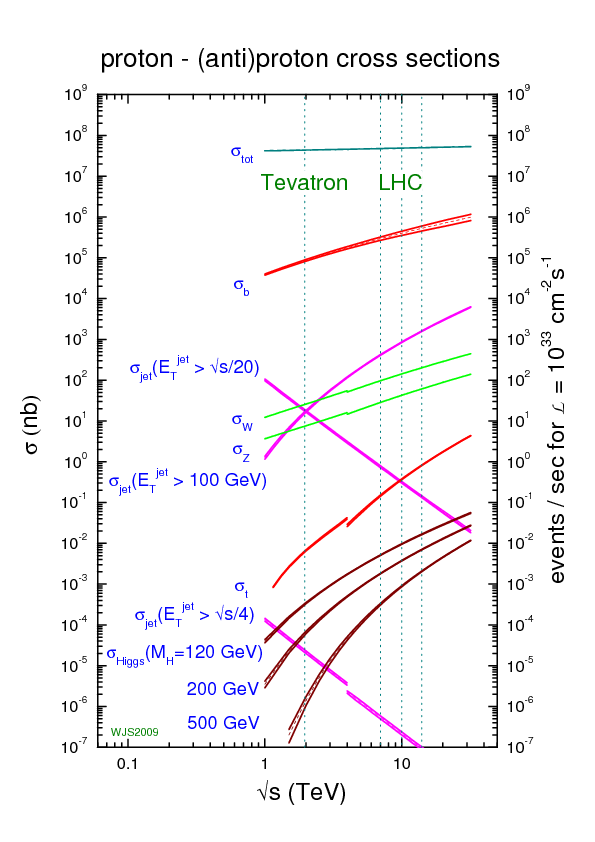
\includegraphics[width=2.9in]{figures/exp_proj/pdf_xsec.png}
\caption{Common cross sections of proton collisions as a function of the center of mass energy $\sqrt{s}$}
\end{center}
\label{fig:pdf_xsec}
\end{figure}

The CMS Trigger System exists as a filter through which events are determined to be ``interesting''. 
It is both  unnecessary and inefficient to record anything that occurs in the detector electronics. 
Most events that occur from colliding protons are well understood. To the left, you can see the 
logarithmic plot of common physics processes for proton-proton scattering. Events such as the production 
of a $b$ quark  occur at $\approx 10^6$ Hz at a luminosity of $\mathcal{L} = 10^{33}$ cm$^{-2}$ 
whereas the production of the Higgs is much lower at $\approx 10^{-2}$ Hz.  \\

At design luminosity, the LHC has beam crossings at a rate of $\approx 40$ MHz with 
each crossing coming spaced at $\approx$ 25 ns. 
For each crossing there are $\approx$ 20 inelastic collisions (referred to as pile up) 
contained in an event file of $\approx$ 1 Mb. 
However the bandwidth for storage is limited to $\approx 10^2$ Hz and equivalently $10^2$ Mb/s. 
Generally, all but one of the inelastic collisions is interesting and a large excess of uninteresting 
activity is generated in the detector electronics. The trigger must be robust enough to select 
this needle in a haystack event while remaining computationally efficient in maximizing the limited bandwidth.  \\

The CMS Trigger system is designed to read events at the event crossing frequency and generate the
 factor $10^5$ of rejection between the crossing frequency and the archival capacity. This factor 
is far too large to achieve in a single step given the complexity of triggers and event reconstruction. 
Therefore the task is split into two steps: The Level 1 (L1) and High Level (HLT) Trigger systems.

The $O(10^7$) events per second first pass through the L1 Trigger which reads out events at $10^5$ Hz. 
From here, the High Level Trigger makes the final decision as to which events are kept. 
Approximately 350 Hz is processed and stored, 300 Hz is ``parked'' (stored but processed later), 
and 1 kHz is partially stored (only the HLT level information and not the RAW detector information) 
and used for data scouting for future analysis.  \\

The most basic criterion for interesting events are hard physics events with high momentum transfer, $q^2$.
 As the protons collide with effectively no transverse momentum, any event with significant deposits of 
transverse energy (or even missing transverse momentum) is indicative of a hard physics process. 
The number of objects with a given transverse momentum falls off exponentially, so a simple minded way to
  reduce the rate of processed events is to raise the threshold of accepted events. \\

More specific criterion for ``interesting events'' is analysis dependent. Generally, analyses are
 categorized by their final state signature. Thus, the trigger requires loose identification 
on the objects of that signature such as the isolation and shape of energy deposition. 
Once the event has passed the Level 1 and HLT Triggers, tighter and more computationally 
costly selection can be made offline where we are unrestricted by bandwidth limitations. \\

As there is a limited amount of bandwidth for processing the events, the numerous analyses of CMS
 are given a budget (measured in Hz) for the triggers they request. As it stands the $H\rightarrow \gamma\gamma$ 
analysis is assigned a budget of 30 Hz for its diphoton trigger suite. As the diphoton channel was of 
high priority in the 7 and 8 TeV running this accounted for a significant fraction ($\approx$10\%) of the overall budget. \\

As the luminosity of the machine increases, we expect proportionally more events per second and must accordingly alter the triggers. 

\begin{figure}
\begin{center}
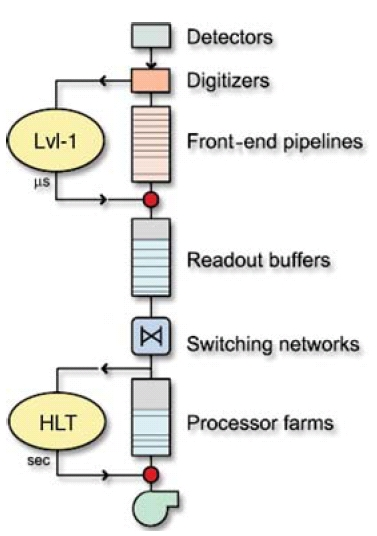
\includegraphics[width=2.5in]{figures/exp_proj/cms-trigger}\\
\caption{A diagrammatic representation of the level 1 and HLT trigger processing}
\end{center}
\end{figure}


\subsubsection{Level 1 (L1) Trigger}

\subsubsection{High Level Trigger (HLT)}


\chapter{The Compact Muon Solenoid Experiment}

Physics from a theoretical point of view can consider particles in terms of their kinematic 
phase space, however we cannot make direct measurements of the hard scattering process. Instead,
detectors are built to indirectly measure the energy and momenta of the final state particles.
To do this, a layered system of sub detectors is used to perform particle identification. 
By relying on known interactions of standard model particles with detector materials 
strong probabilitistic statements can be made the flavor of particles in a given collision. 
By building a heremetic detector and integrating the various subdetectors in a given 
solid angle, one obtains a wholeistic view of the fundamental physics.
This chapter will discuss each subdetector, the particles it is used to identify, and the 
underlying physics which allows the individual measurements to be made.


The Compact Muon Solenoid (CMS) Detector is a general-purpose detector consisting of 
an all silicon tracker, a precision electromagnetic calorimeter (ECAL), a hadron calorimeter
 (HCAL), a 4 T superconducting solenoid and muon chambers. The solenoid deflects charged
 particles whose paths are traced in the tracker, making it possible to 
reconstruct the particles’ momentum. The two calorimeters reconstruct the energy 
of and identify photons, electrons and hadronic jets.
As shown in Figure \ref{fig:cms} the detector has cylindrical symmetry about the
 interaction point where the proton beams collide. By maintaining near full coverage 
of the interaction point it is possible to detect signatures such as neutrinos or other 
weakly interacting particles as missing energy. 


\begin{figure}
\begin{center}
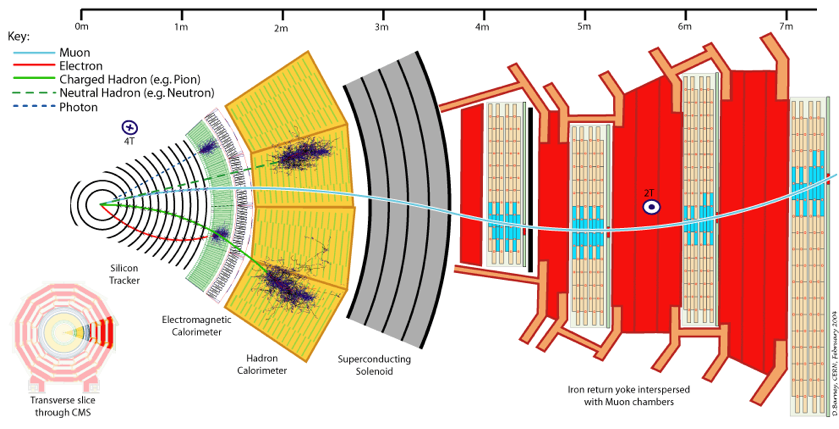
\includegraphics[width=.95\textwidth]{pics/cms_transverse}
\end{center}
\caption{ A tear-away view of the inner detectors of CMS.}
\label{fig:cms_transverse}
\end{figure}

\begin{figure}
\begin{center}
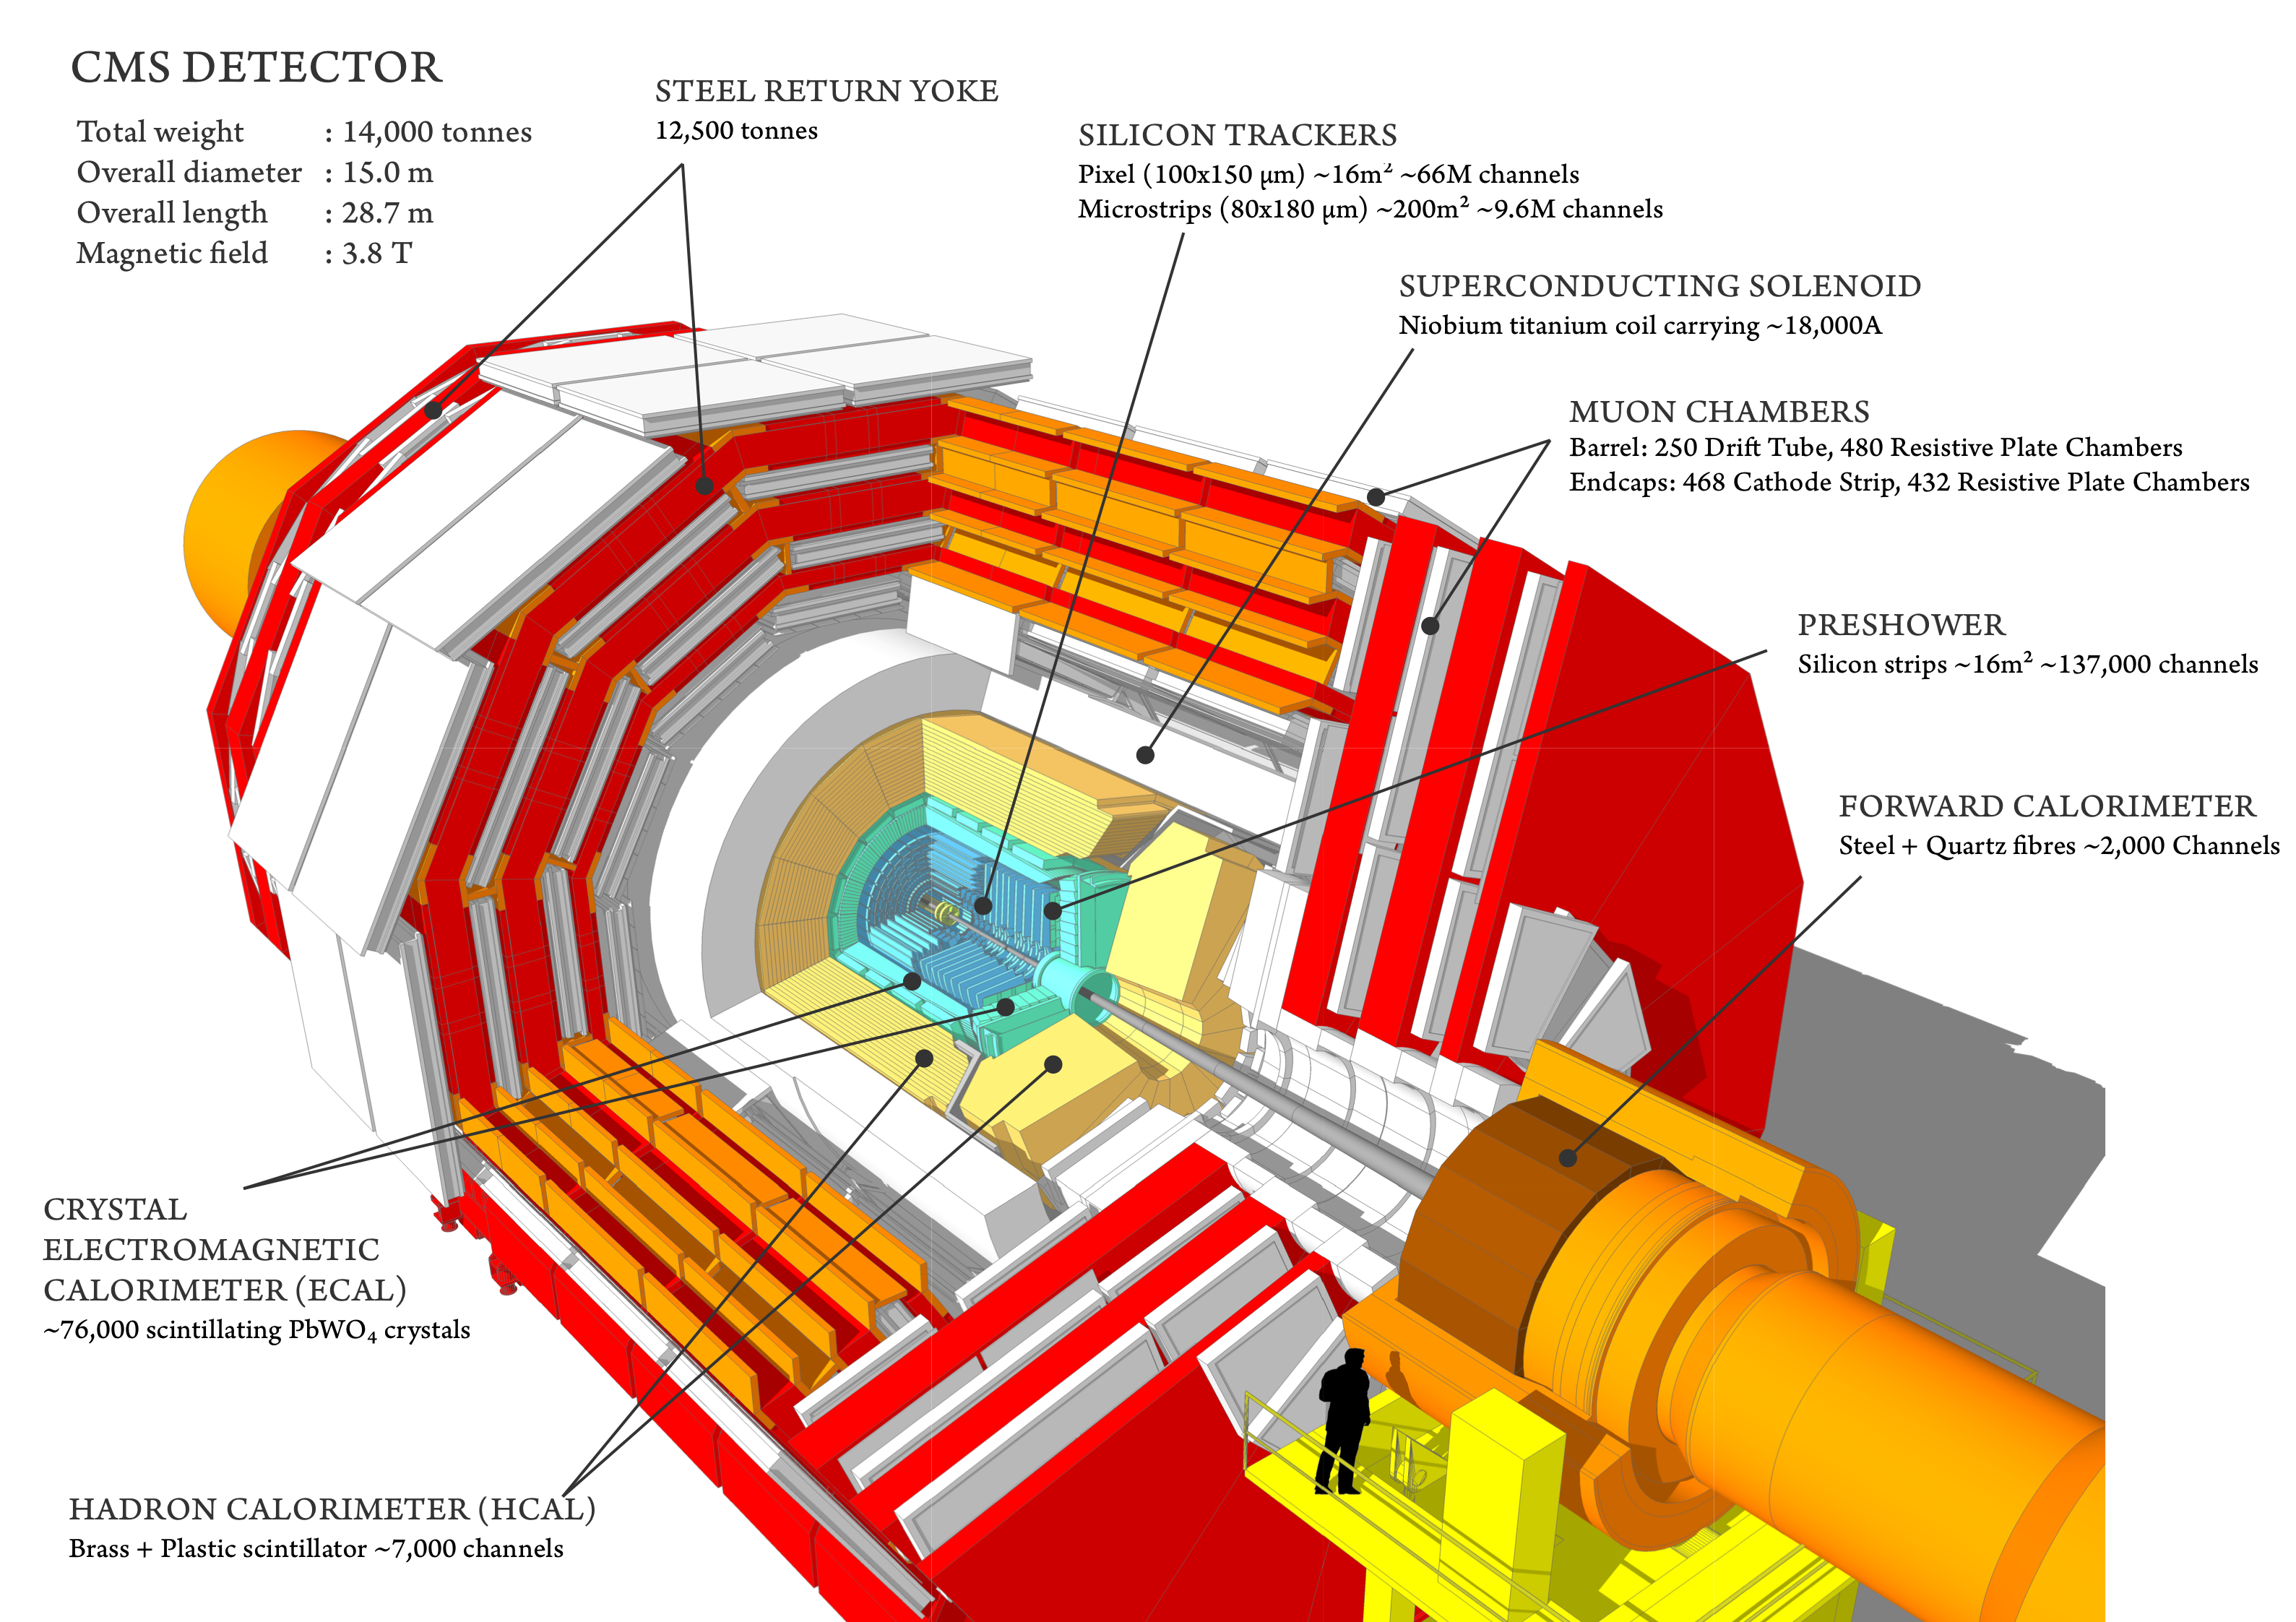
\includegraphics[width=.90\textwidth]{pics/cut_away_view}
\end{center}
\caption{Cut away view of the CMS Detector}
\label{fig:cms_onion}
\end{figure}



\section{Superconducting Solenoid}


\begin{figure}
\begin{center}
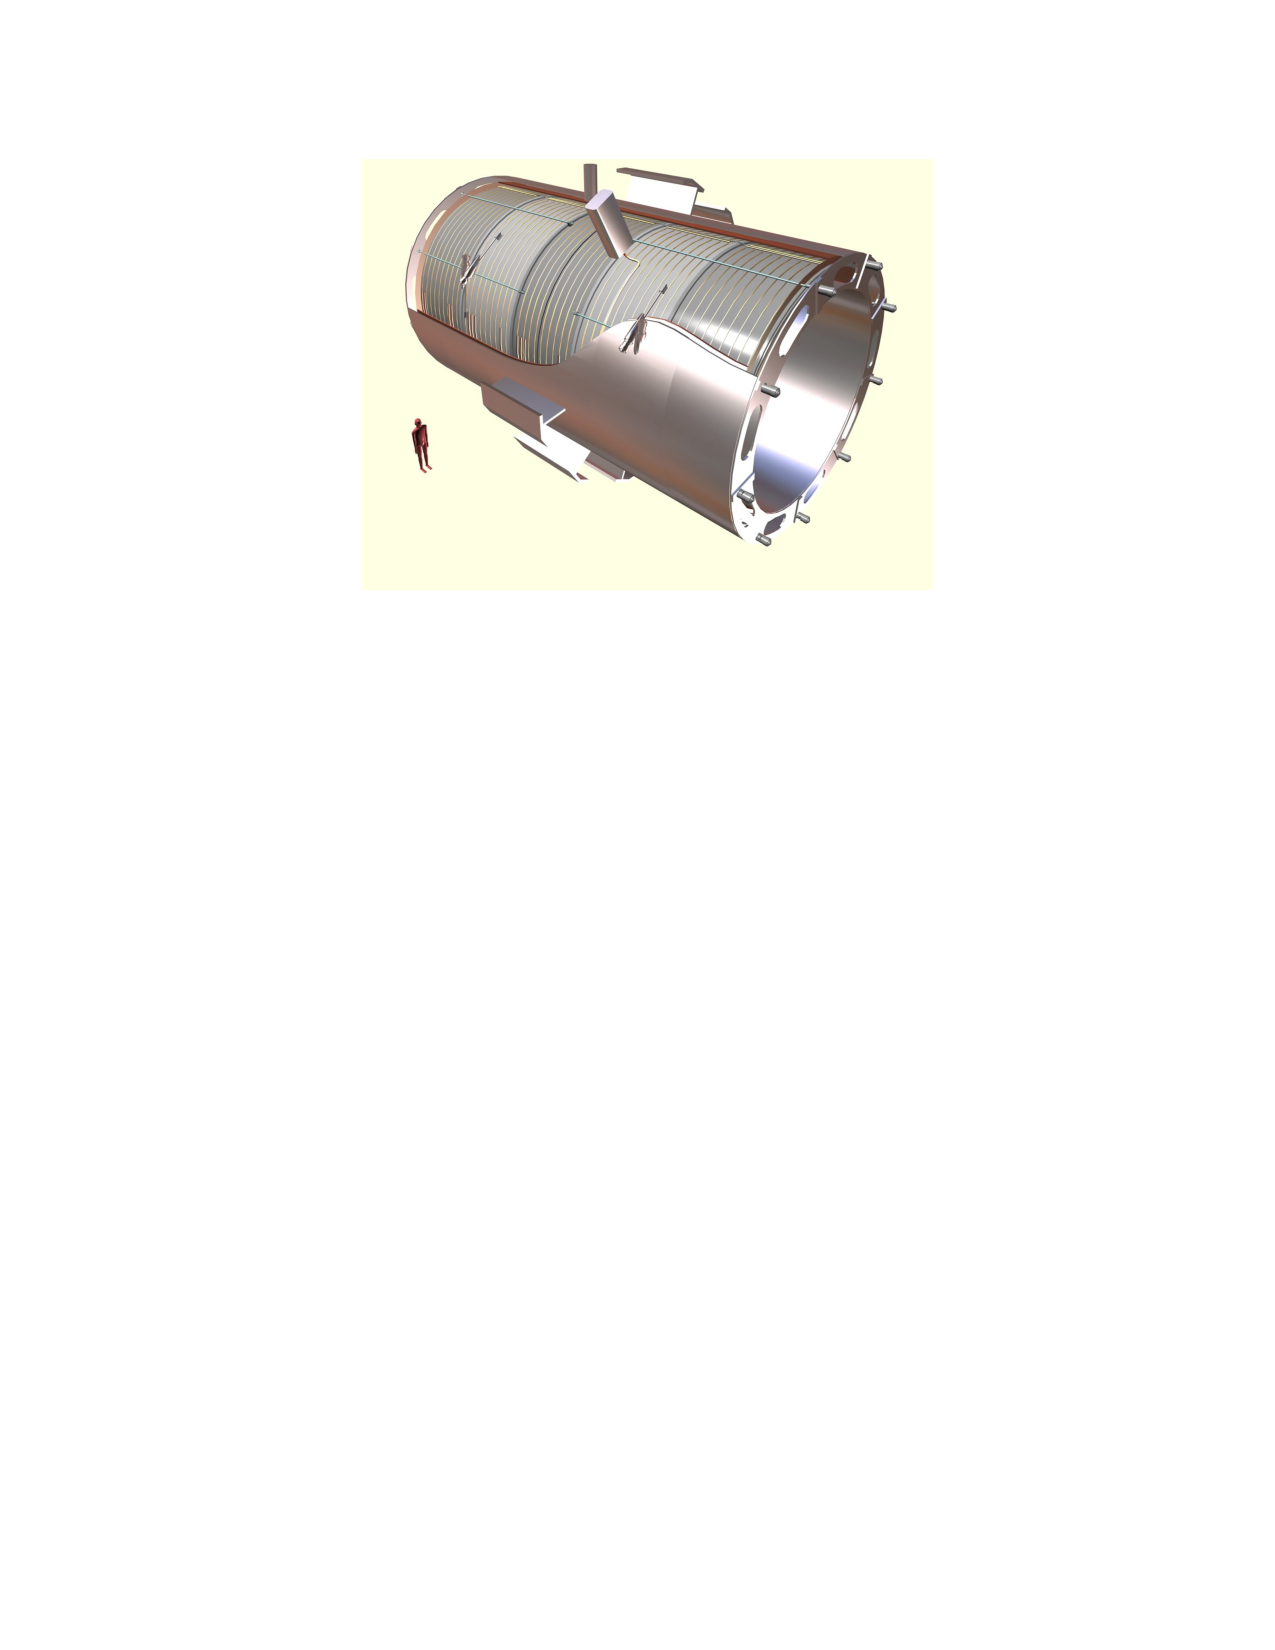
\includegraphics[width=.45\textwidth]{pics/solenoid_diagram}
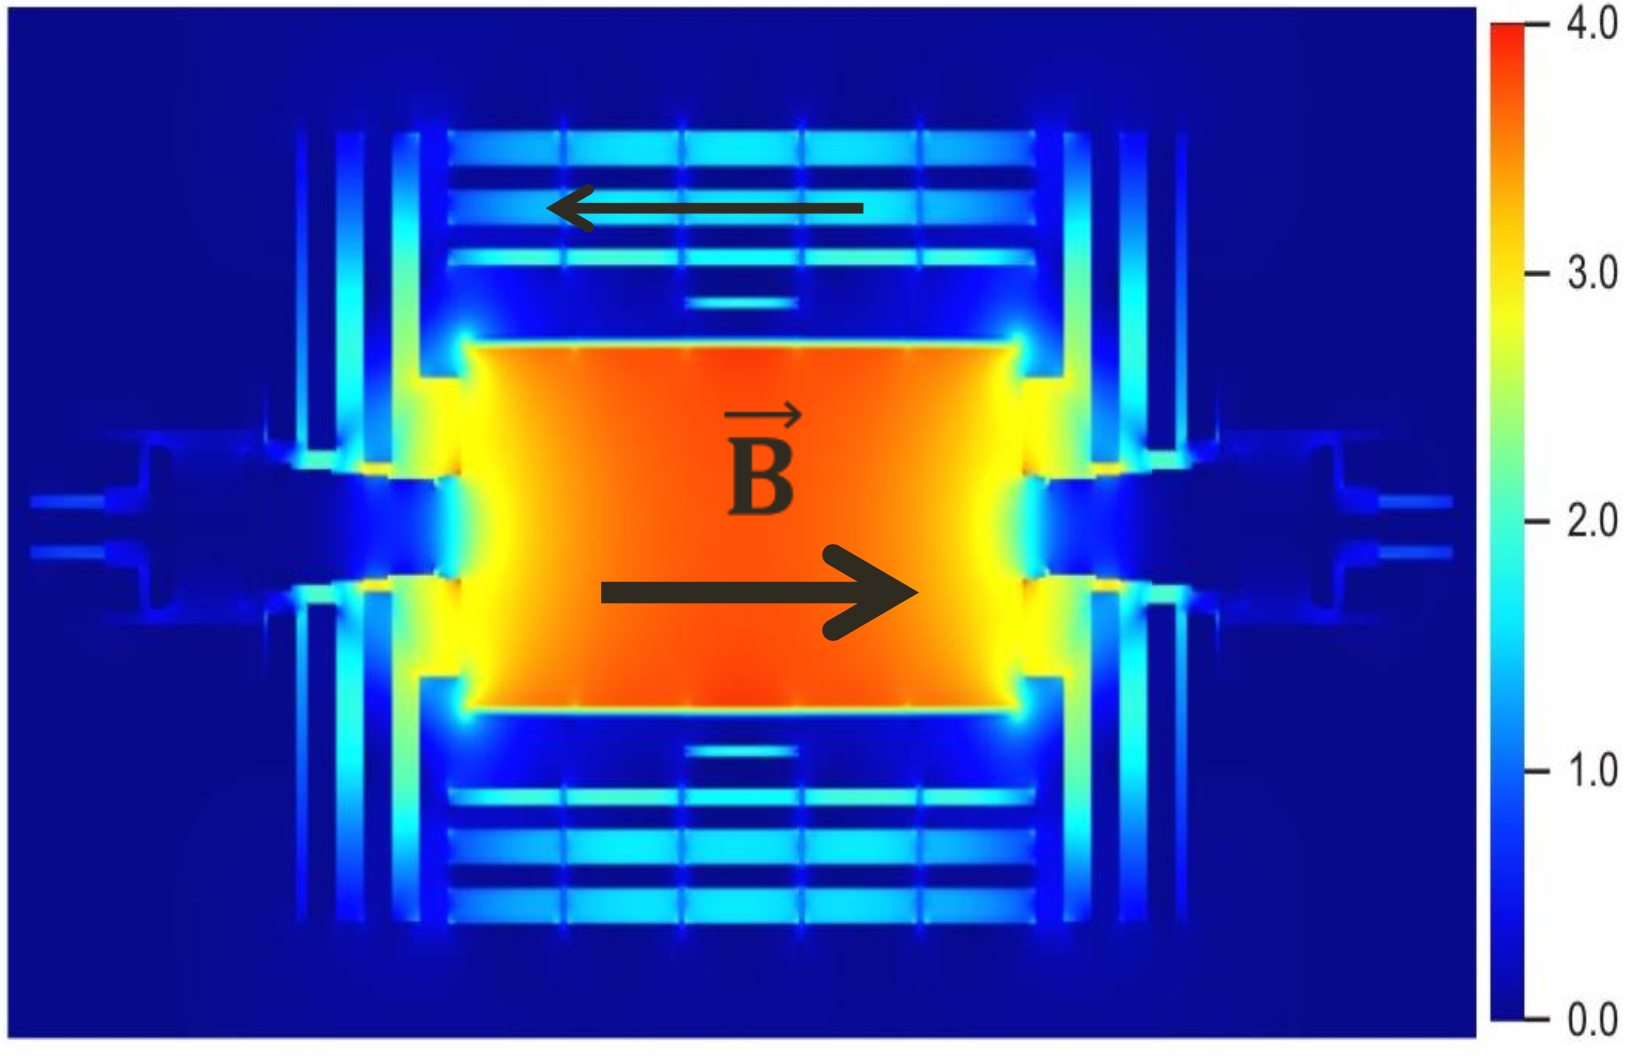
\includegraphics[width=.45\textwidth]{pics/b_field}
\end{center}
\caption{The CMS solenoid with a human for scale}
\label{fig:solenoid_bfield}
\end{figure}

It is worth beginning this discussion with the central feature the rest of the detector is built, the 
design 4 T  superconducting solenoidal magnet. For scale, a typical refridgerator magnet is on the 
order of $10^{-2}$ T and the MRI magnets can range between 0.5-3.0 T. The magnetic field is used
to measure the momentum of charged particles by bending their trajectories. As the size of the bend is
proportional to the field and inversely to the momentum of the particle, a stronger field is required 
to measure higher energy particles. 

\begin{figure}
\begin{center}
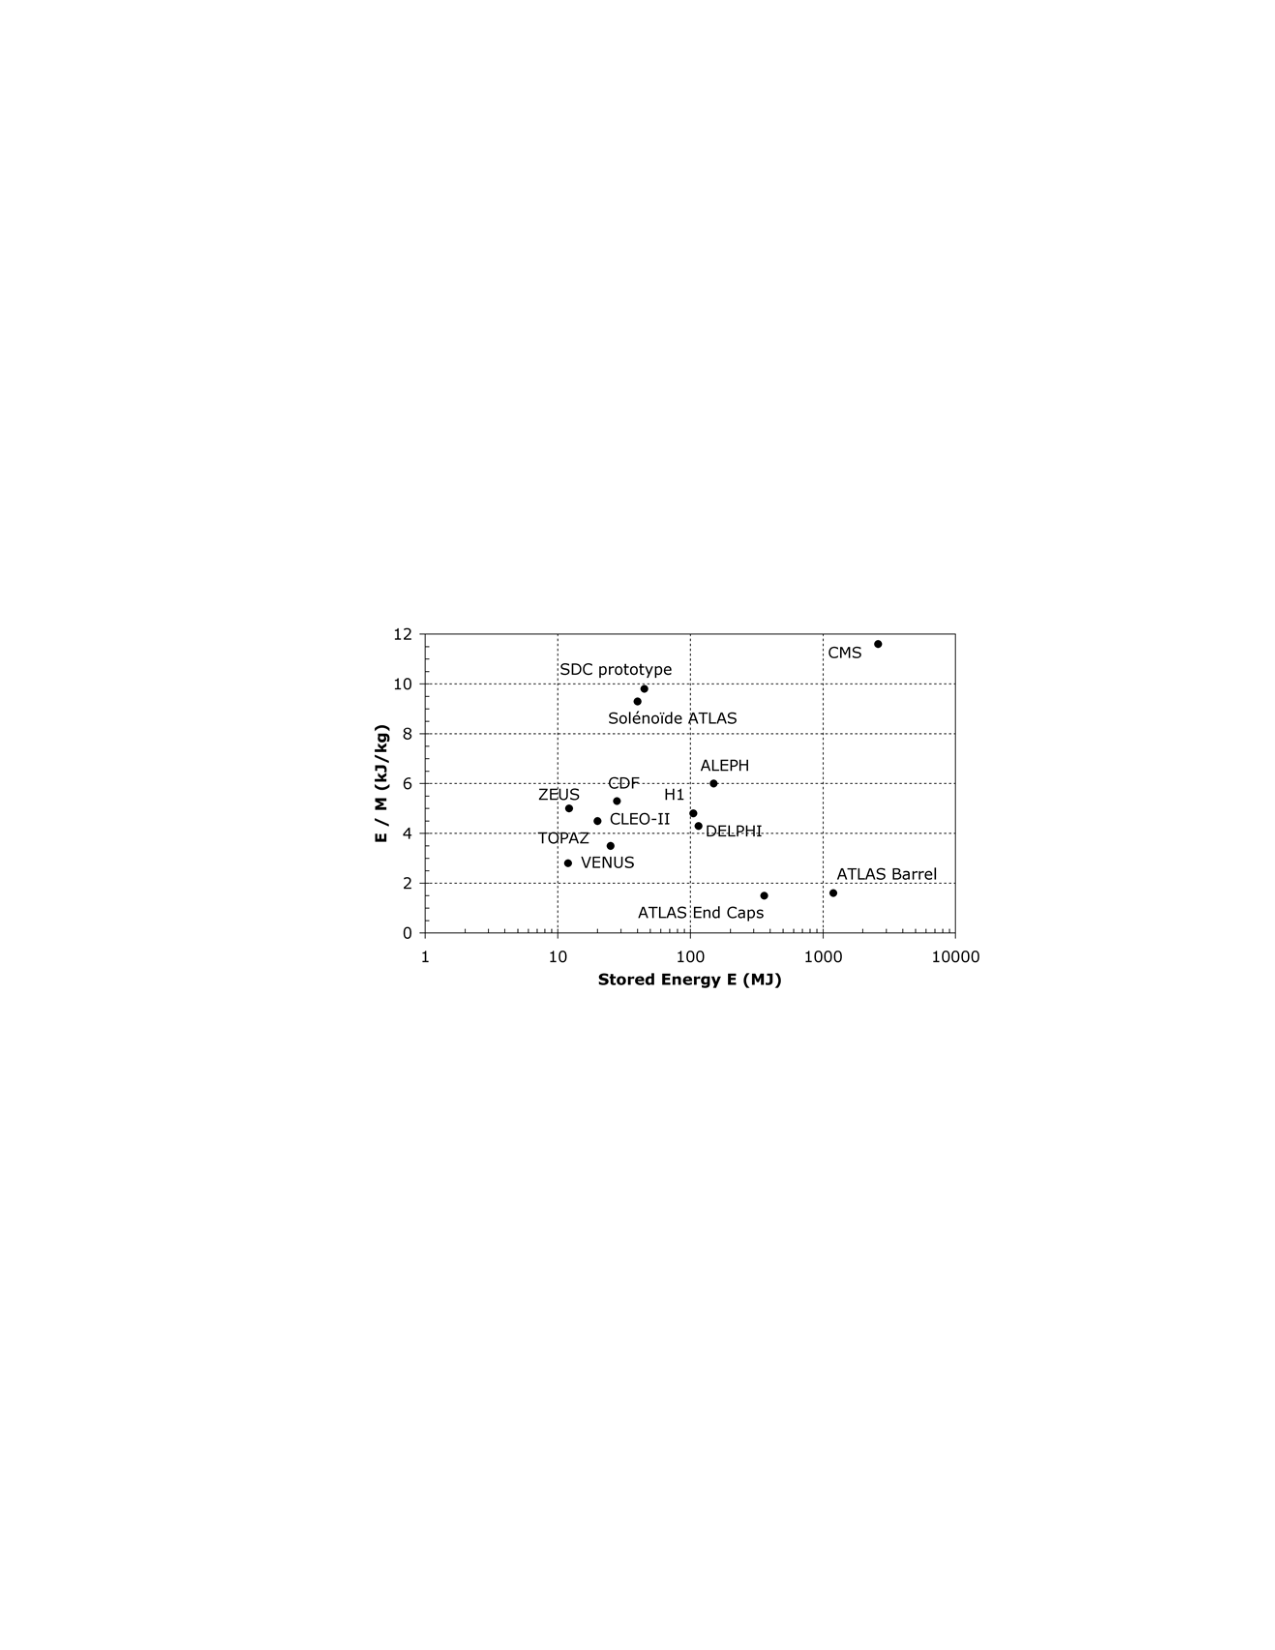
\includegraphics[width=.75\textwidth]{pics/CMS_EoverM}
\end{center}
\caption{The CMS solenoid with a human for scale}
\label{fig:eoverm}
\end{figure}

The magnet is 6 meters in diameter with 12.5 meters in length. The magnetic field is generated 2180 turns 
wound in four layers of Niobium Titanium conductors inside an alumninum cylinder carrying a
 nominal current of 20 kA.  At the design field strength the solenoid a stores magnetic field of 
2.66 GJ, the largest stored energy of any magnet ever built. The energy to mass ratio is 11.6 kJ/kG a indentifying 
feature in the historical context of detector magnets (Figure \ref{fig:eoverm}).    

\begin{figure}
\begin{center}
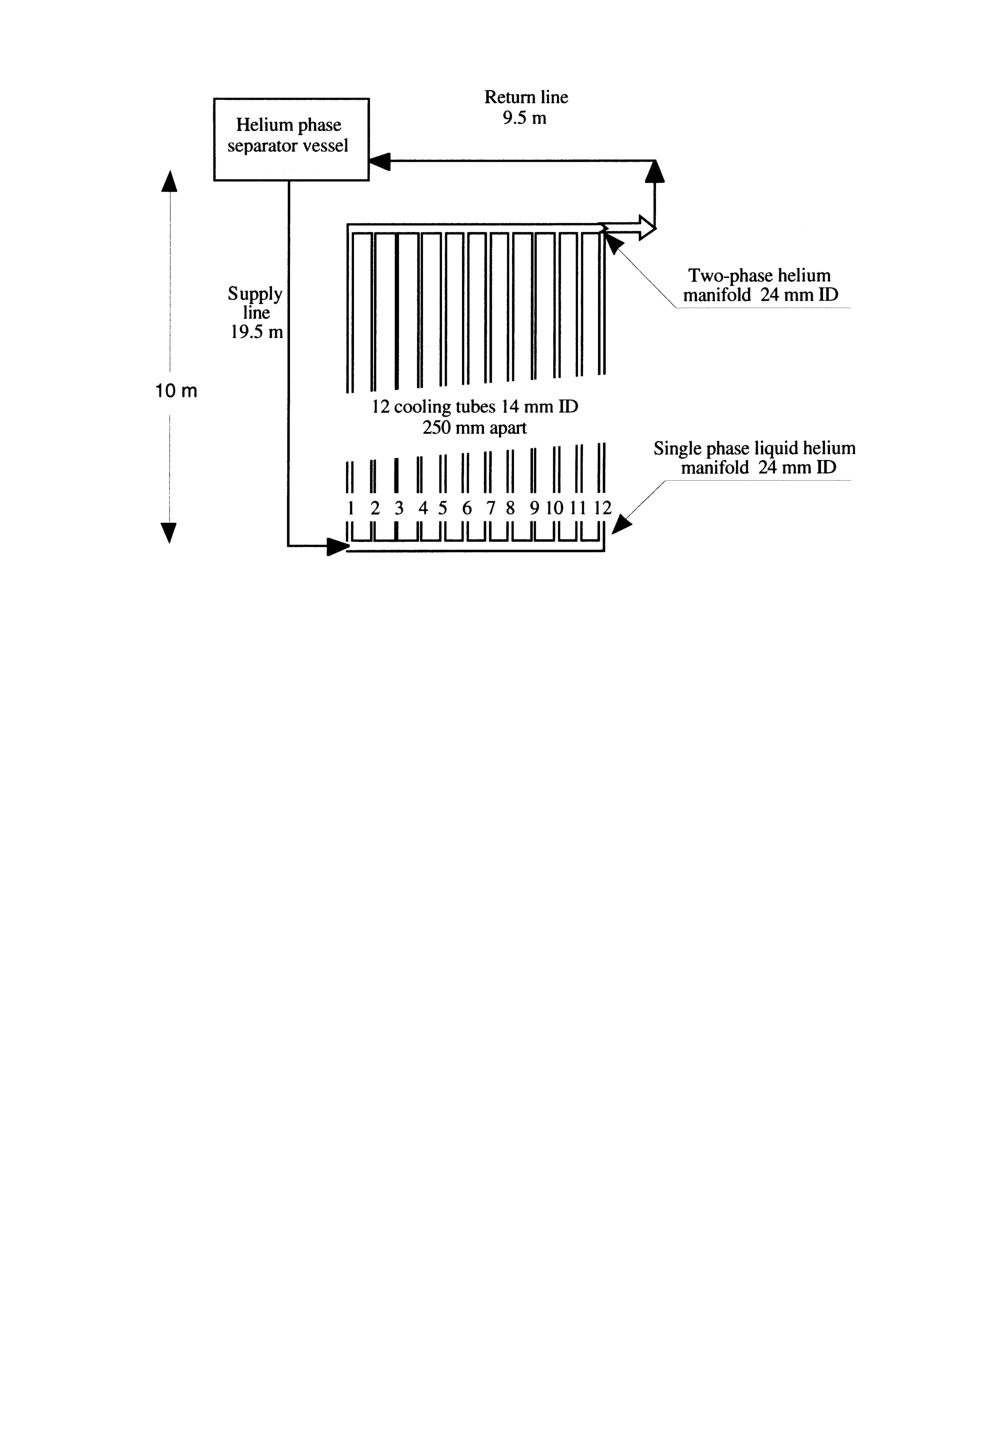
\includegraphics[width=.55\textwidth]{pics/thermosiphon}
\end{center}
\caption{A sub circuit of the CMS thermosiphon}
\label{fig:eoverm}
\end{figure}

To operate in a superconducting state, the system is cooled  4.5 K with a thermosiphon
 (cite-quench-production). A thermosiphon is an indirct cooling method utilizing passive heat exchange where
rather than pumping the liquid helium the flow is induced thermally. 

The system requires 3 days to 
reach cool the system from room to operating temperature. 

The magnet is supplemented by a iron return yoke to



\section{Electromagnetic Calorimeter (ECAL)}


\begin{figure}
\begin{center}
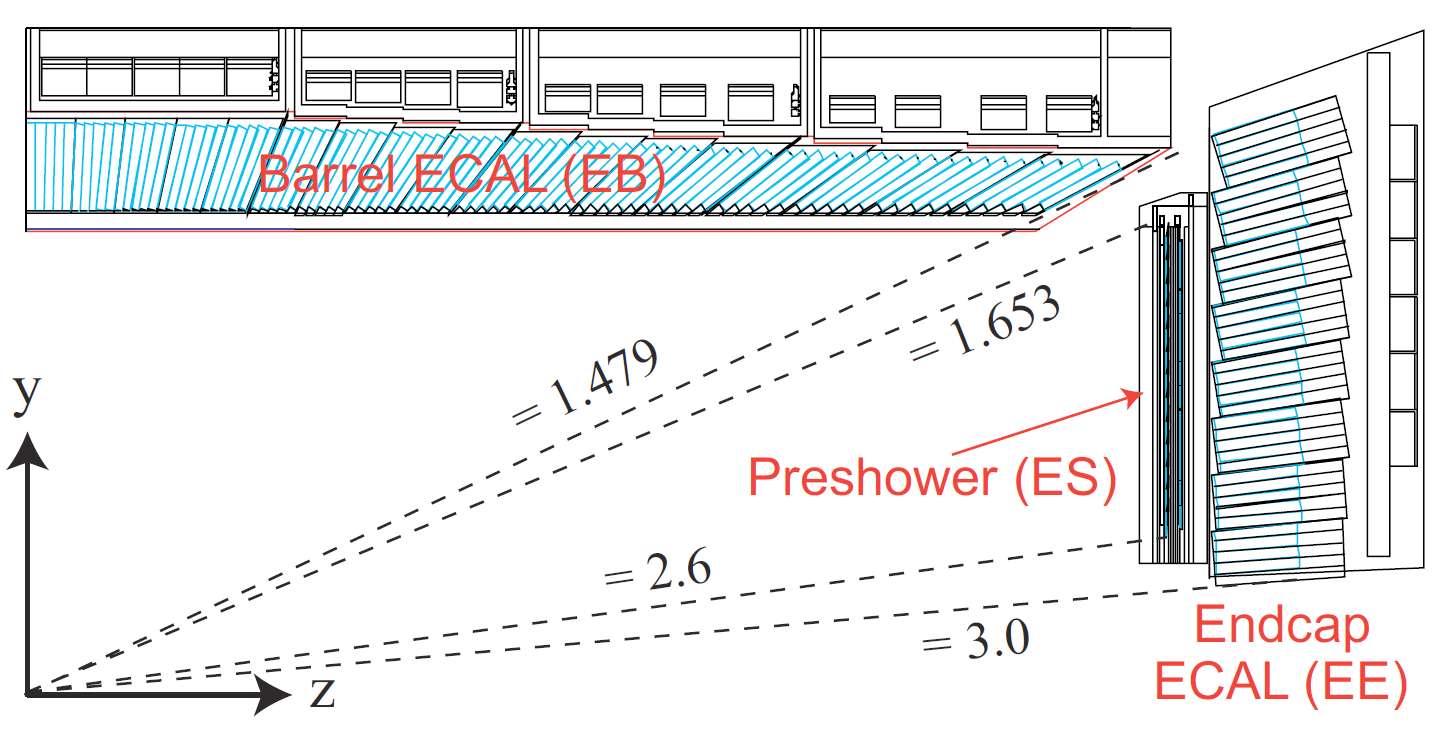
\includegraphics[width=.95\textwidth]{pics/ecal_diagram_side}
\end{center}
\caption{Kinematic coverage of the electromagnetic calorimeter (ECAL) barrel and endcap}
\label{fig:ecal}
\end{figure}

The electromagnetic calroimeter (ECAL) exists to measure the energy of eletromagnetic
showers of electrons and photons.  

For high energy electromagnetic objects, that is above the mass threshold of 
pair production: $\gamma \rightarrow e^+e^-$, the interaction with matter occurs as an electromagnetic shower. In this shower, photons pair produce electron-positon pairs and
 electrons undergo bremmstrahlung 
radiation: $e^\pm \rightarrow \gamma e^\pm$. This processes continues until 
the individual particles in the shower cannot continue $1\rightarrow 2$
 processes and instead undergo multiplicity presverving iteractions such 
as compton scattering and ionization.

The detector material (for CMS a scintillating crystal) is characterised the shower's
 Moliere Radius, defined as the radius
 (transverse to the incidence) of a cylinder that contains 90\% of the shower. For the CMS ECAL, 
crystals are of approximately the Moliere radius 2.2 cm. The material can further
be characterized by it's radiation length, the typical amount of matter the incidient particle
can traverse before an interaction. The CMS crystals have a relatively short radiation
 length of 0.9 cm. Each crystal is approximately 25 radiation lengths = 23 cm. 

The cystal energy resolution as a function of energy is characterised as:
\begin{equation}
\frac{\sigma(E)}{E} = \frac{S}{\sqrt{E}} \oplus \frac{N}{E} \oplus C
\end{equation}
Here $\sigma$ is the gaussian standard deviation of the energy measurement, the operator $\oplus$ signifies addition in quadrature, $S$ the stochastic term, $N$ the
electronic readout noise, and $C$ the constant term which does not scale with energy. The 
stochastic term $S$ comes from the staistical nature of the photoelectric shower and the 
containment within the crystal. The readout term arises from the electronics noise in the preamplifier and digitization of the signal. The constant term $C$ is caused by non uniformities between
the many crystals and is ultimately dominated by the crystal to crystal intercalibration. As
the first two term scale inversely with energy the constant term for high energy photons and electrons $> 50$ GeV is dominant. The design energy resolution for high energy photons like those
found in the discovery of the Higgs bosom is $< 0.5\%$

\begin{figure}
\begin{center}
%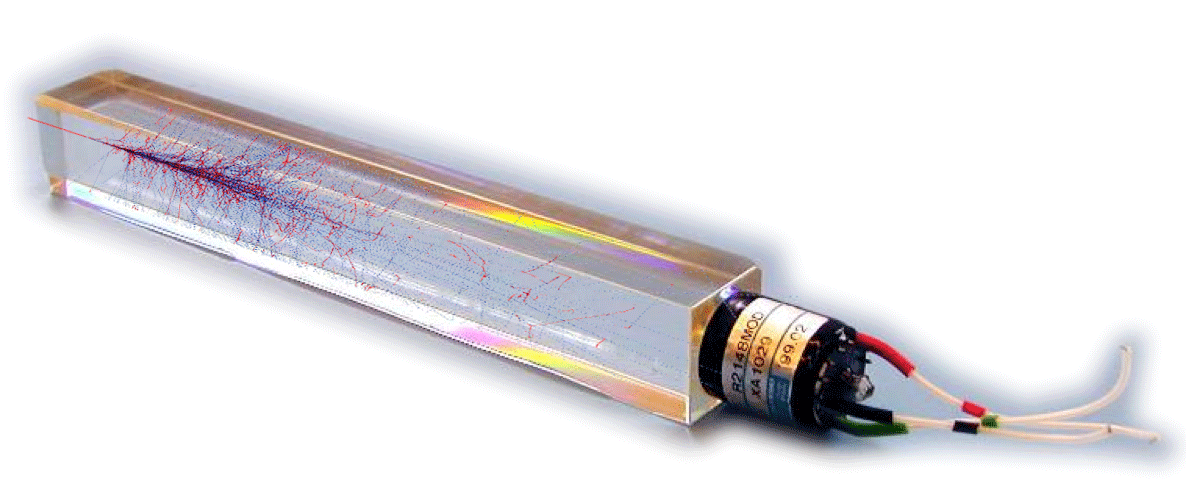
\includegraphics[width=.45\textwidth]{pics/ecal_crystal}
%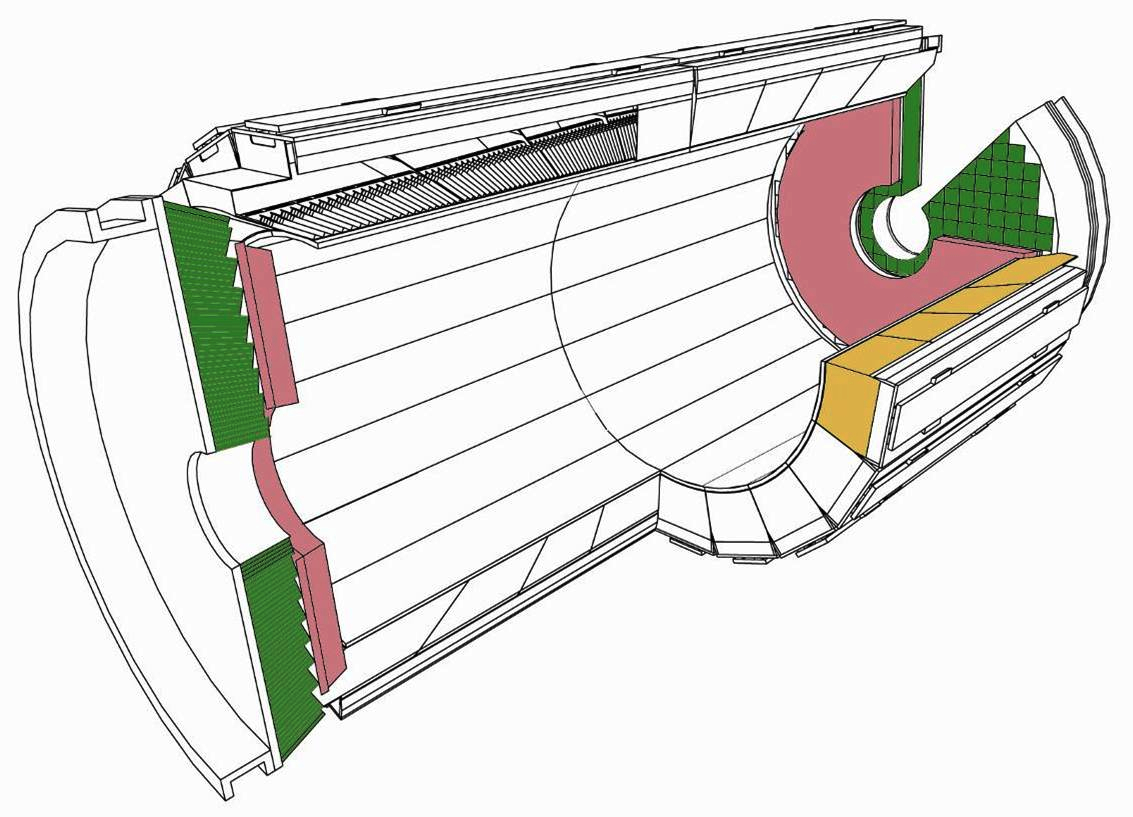
\includegraphics[width=.45\textwidth]{pics/ecal_diagram}
%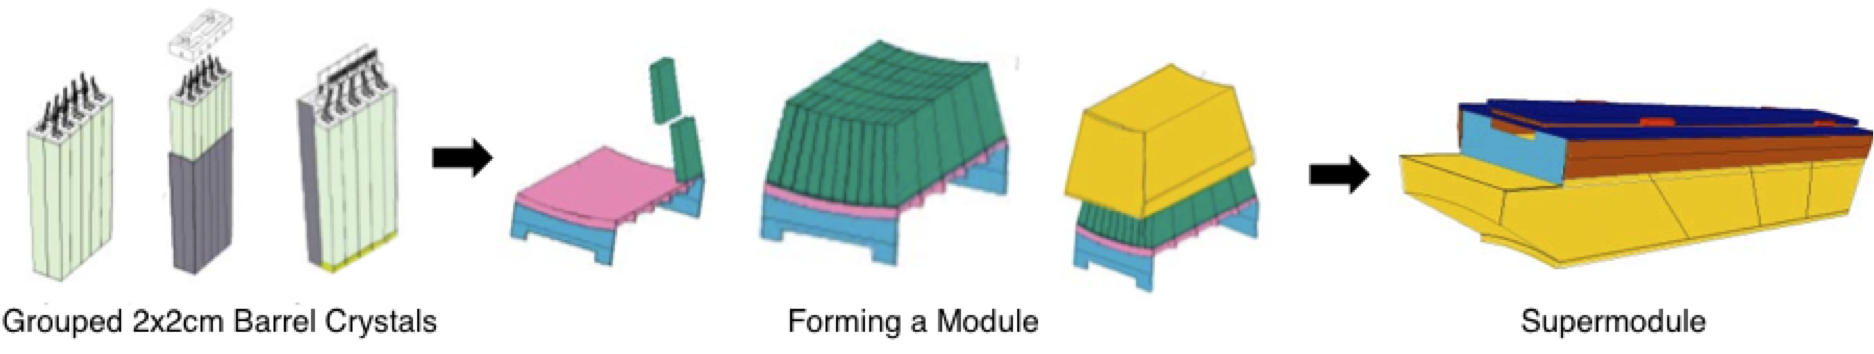
\includegraphics[width=.95\textwidth]{pics/Supermodule}
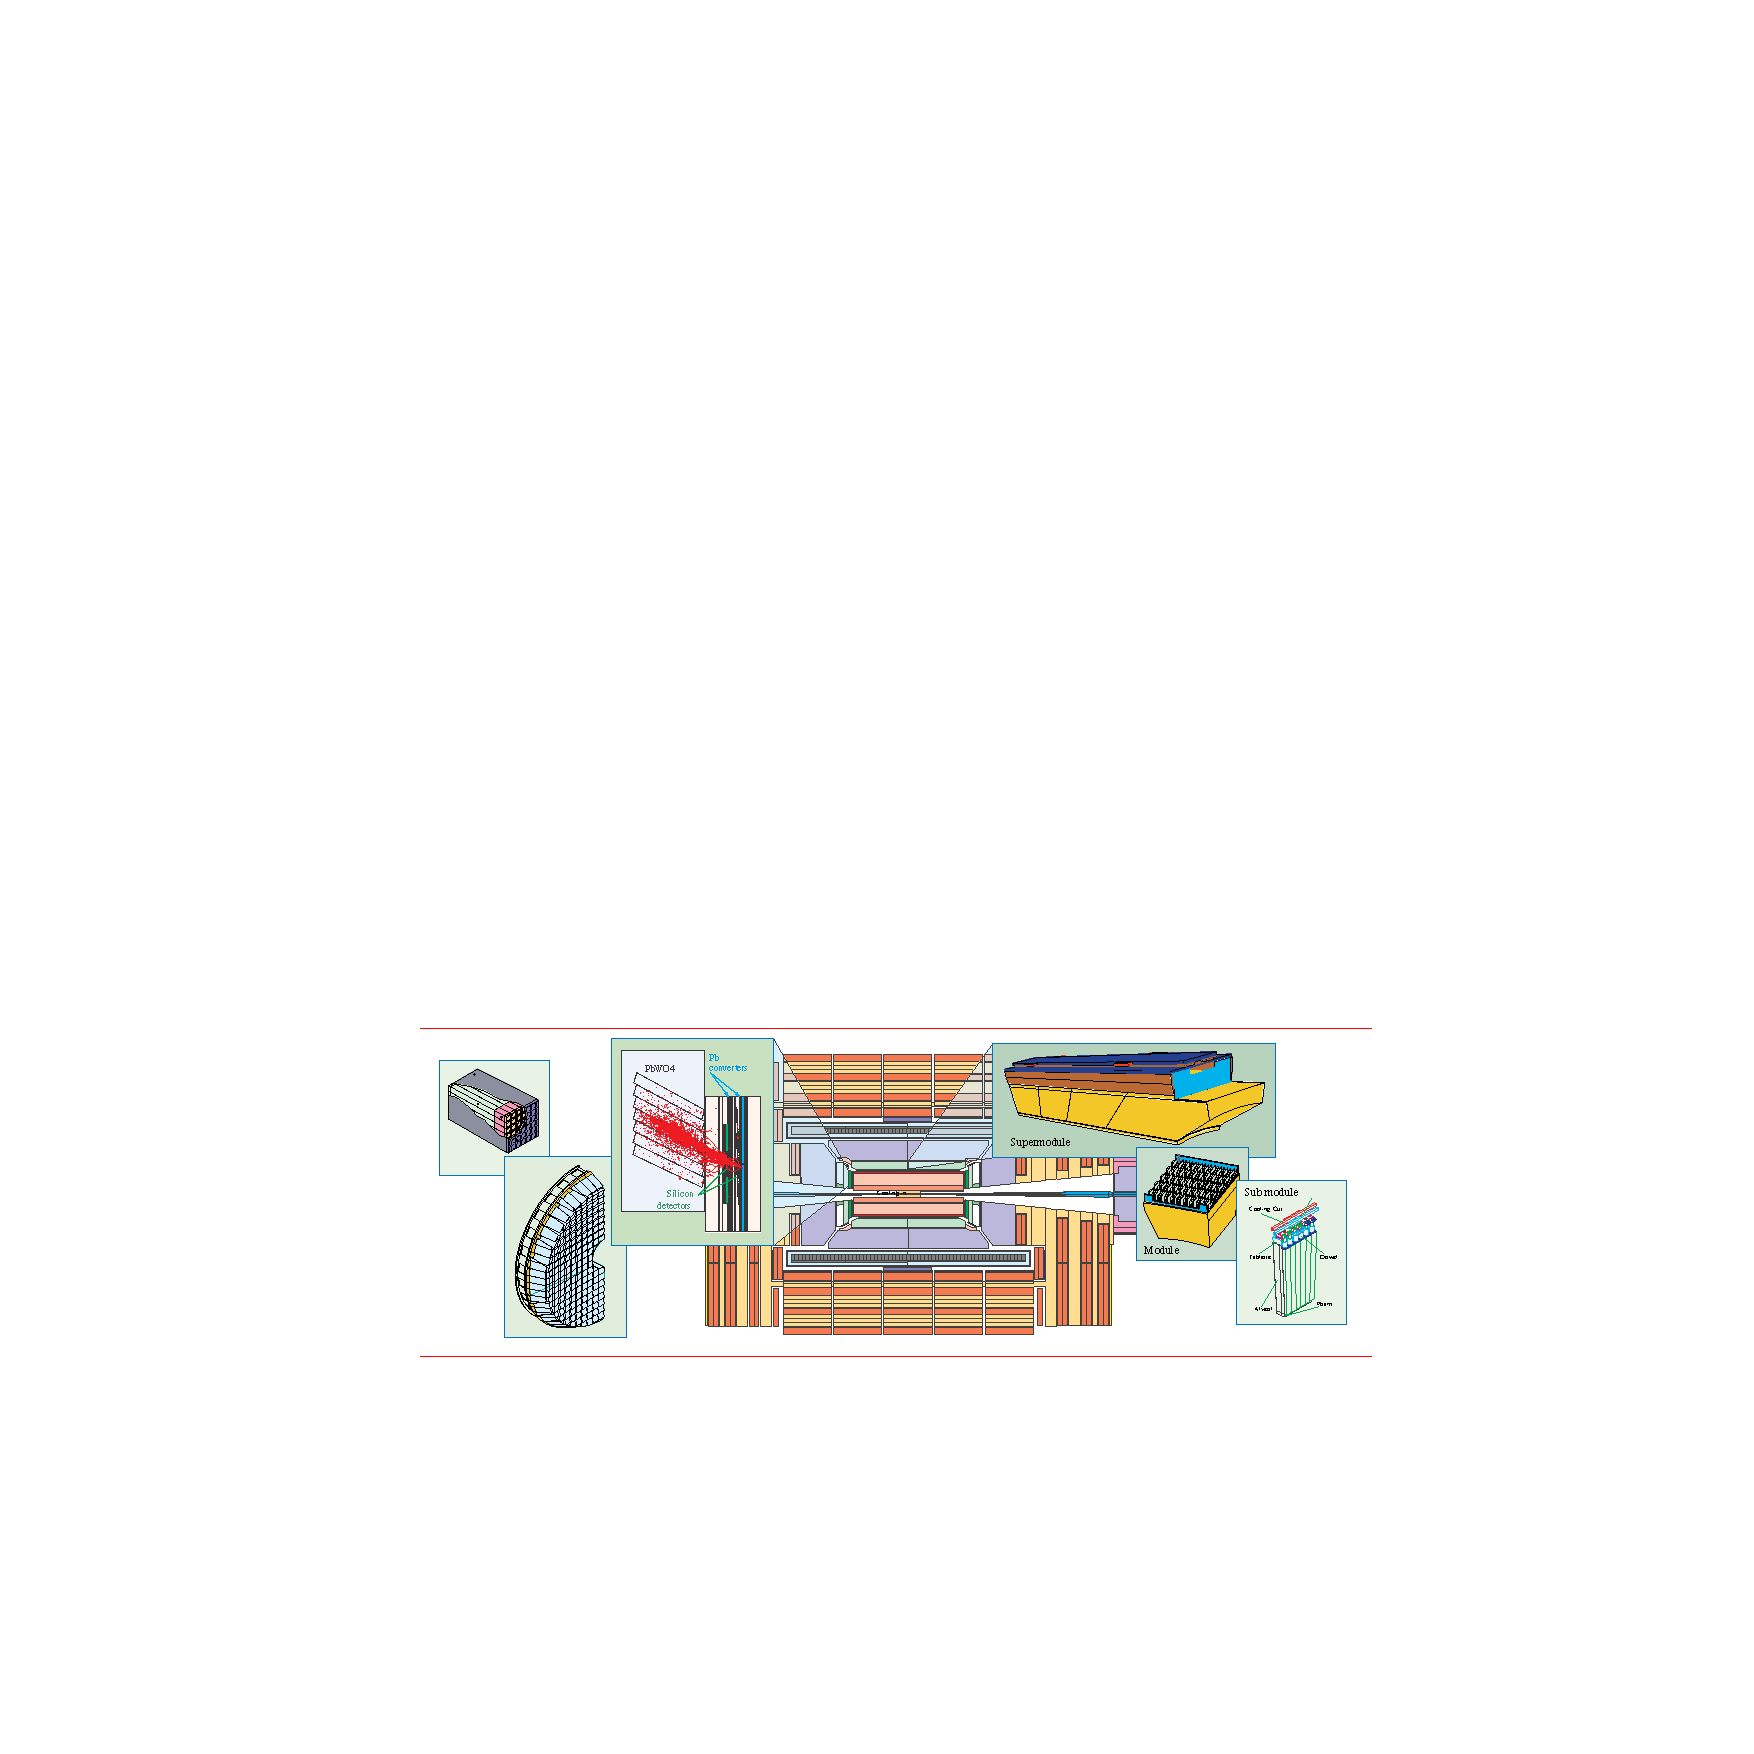
\includegraphics[width=.95\textwidth]{pics/cms_ecal_parts}
\end{center}
\caption{A single CMS ECAL Crystal (top left) tearaway view of distribution of crystals (top right) The construction of a single supermodule (bottom)   }
\label{fig:ecal_cryastal}
\end{figure}

\begin{figure}
\begin{center}
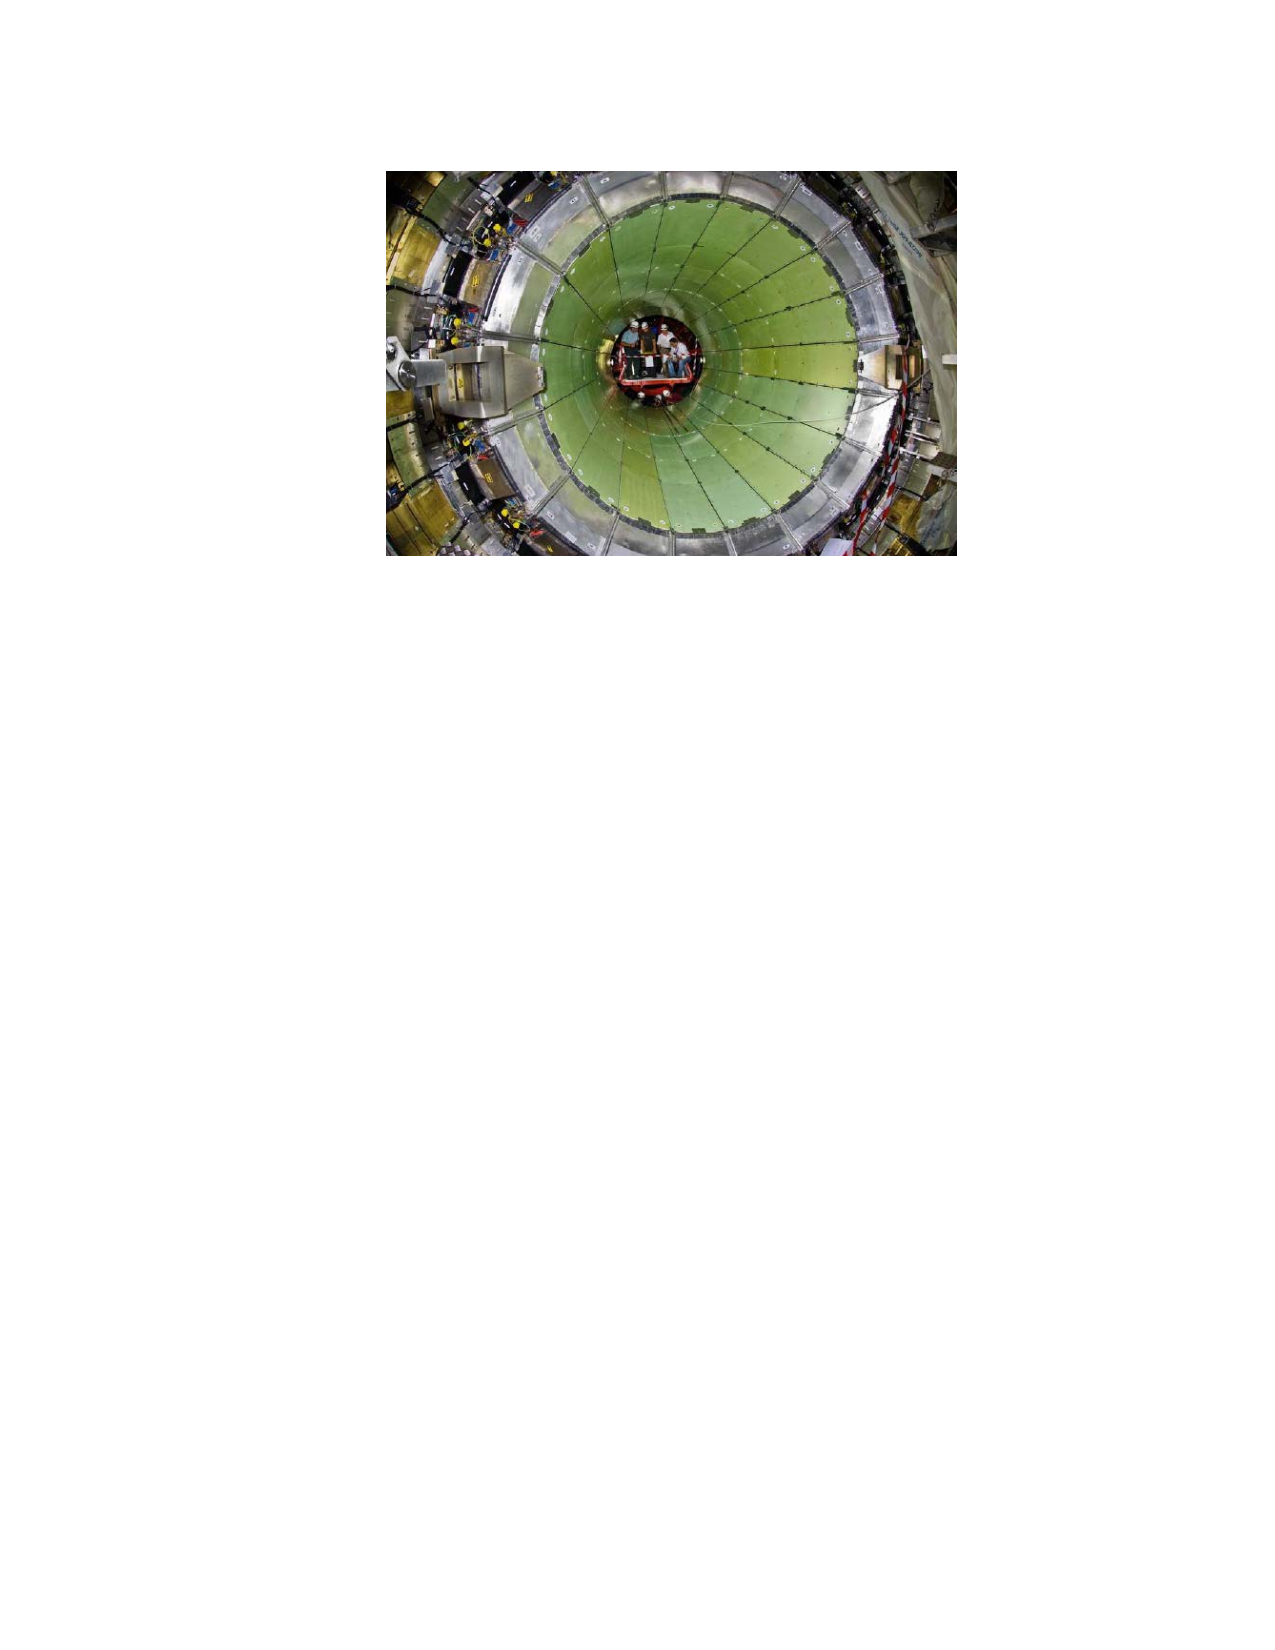
\includegraphics[width=.45\textwidth]{pics/ecal_barrel}
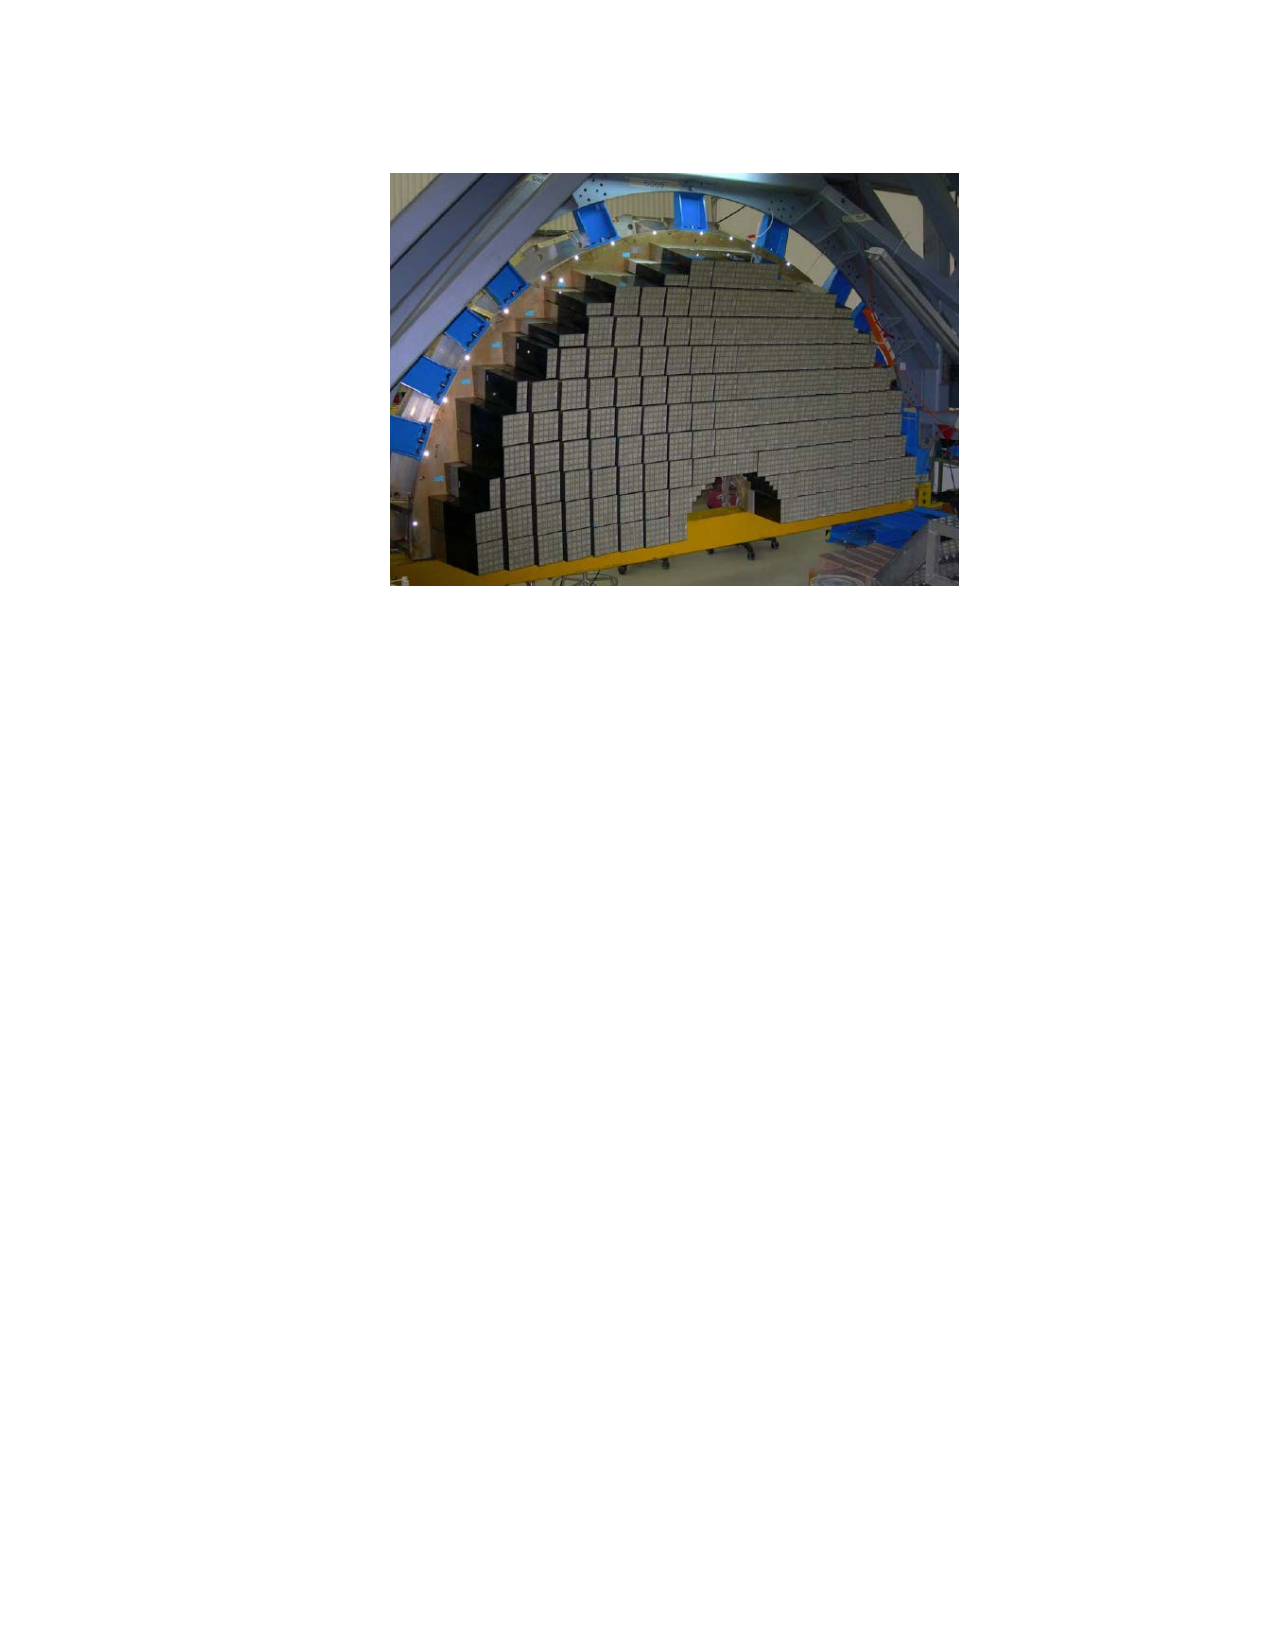
\includegraphics[width=.45\textwidth]{pics/ecal_dee}
\end{center}
\caption{The ECAL barrel installed within CMS (left) A single Dee of the ECAL endcap (right)}
\label{fig:ecal_photos}
\end{figure}

The ECAL consists of 75,848 Lead Tungstate PbWO$_4$ scintillating crystals Fig. \ref{fig:ecal_crystal}. The ECAL is separated into two sections: the Endcaps and the Barrel. 
The Barrel consists of 61200 2x2x23 cm$^3$ crystals separated into 36 Supermodules  and is contained in $|\eta| < 1.48$. The Endcaps are separated into 4 Dees (Fig. \ref{fig:ecal_photos})
 of 3662 crystals with each crystal measuring 3x3x22 cm. 
The 4 dees cover a  pseudorapidity range between $1.48 < |\eta| < 3.0$.
The Endcaps are behind a preshower detector, composed of two lead absorbers 
interleaved with silicon detectors. The preshower covers the pseudorapditiy range
of $1.653 < |\eta| < 2.6$ with each silicon sensor covering a square are of 
63 mm x 63 mm divided into 32 strips. The preshower is designed to give significantly
better spatial resolution than using the endcap alone to aid in the separating single photons
and $\pi^0 \rightarrow \gamma\gamma$ decays used to calibrate the endcap. As the first layer is
2 radiation wavelengths thick such that the majoirty of incident single photons will  
begin to shower before reaching the second layer.  


The preshower converts many of the photons, 
which assists in distinguishing directly produced photons from pairs
of photons resulting from neutral pion decays. 

The light in each crystal is collected as a current 
and amplified by avalanche photodiodes (APDs) in the barrel
region and vaccuum phototriodes (VPTs) in the endcap. This transition is
necessary as the endcap region must be tolerant to much
higher levels of radiation damage from softly scattered (low momentum transfer $Q^2$)
interactions. 

\begin{figure}
\begin{center}
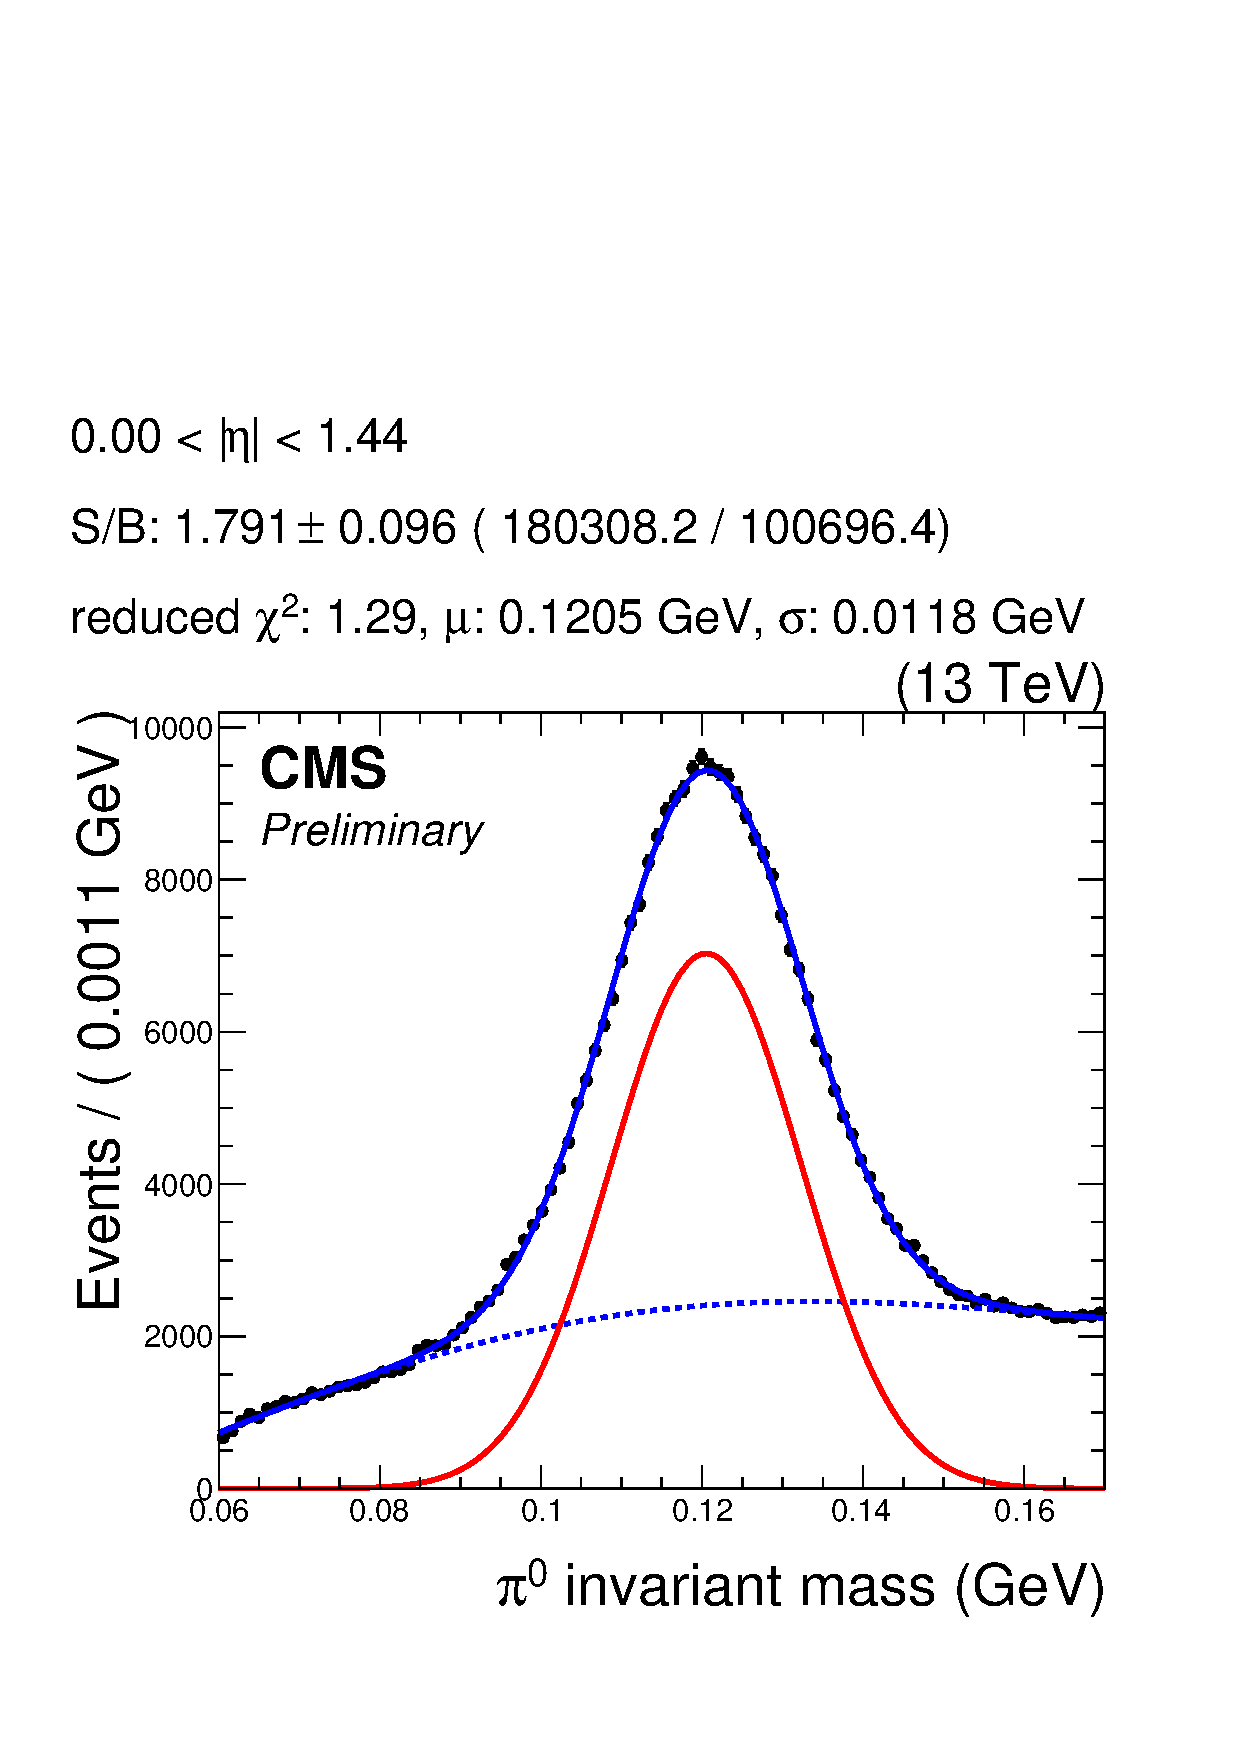
\includegraphics[width=.45\textwidth]{pics/pizero_eb}
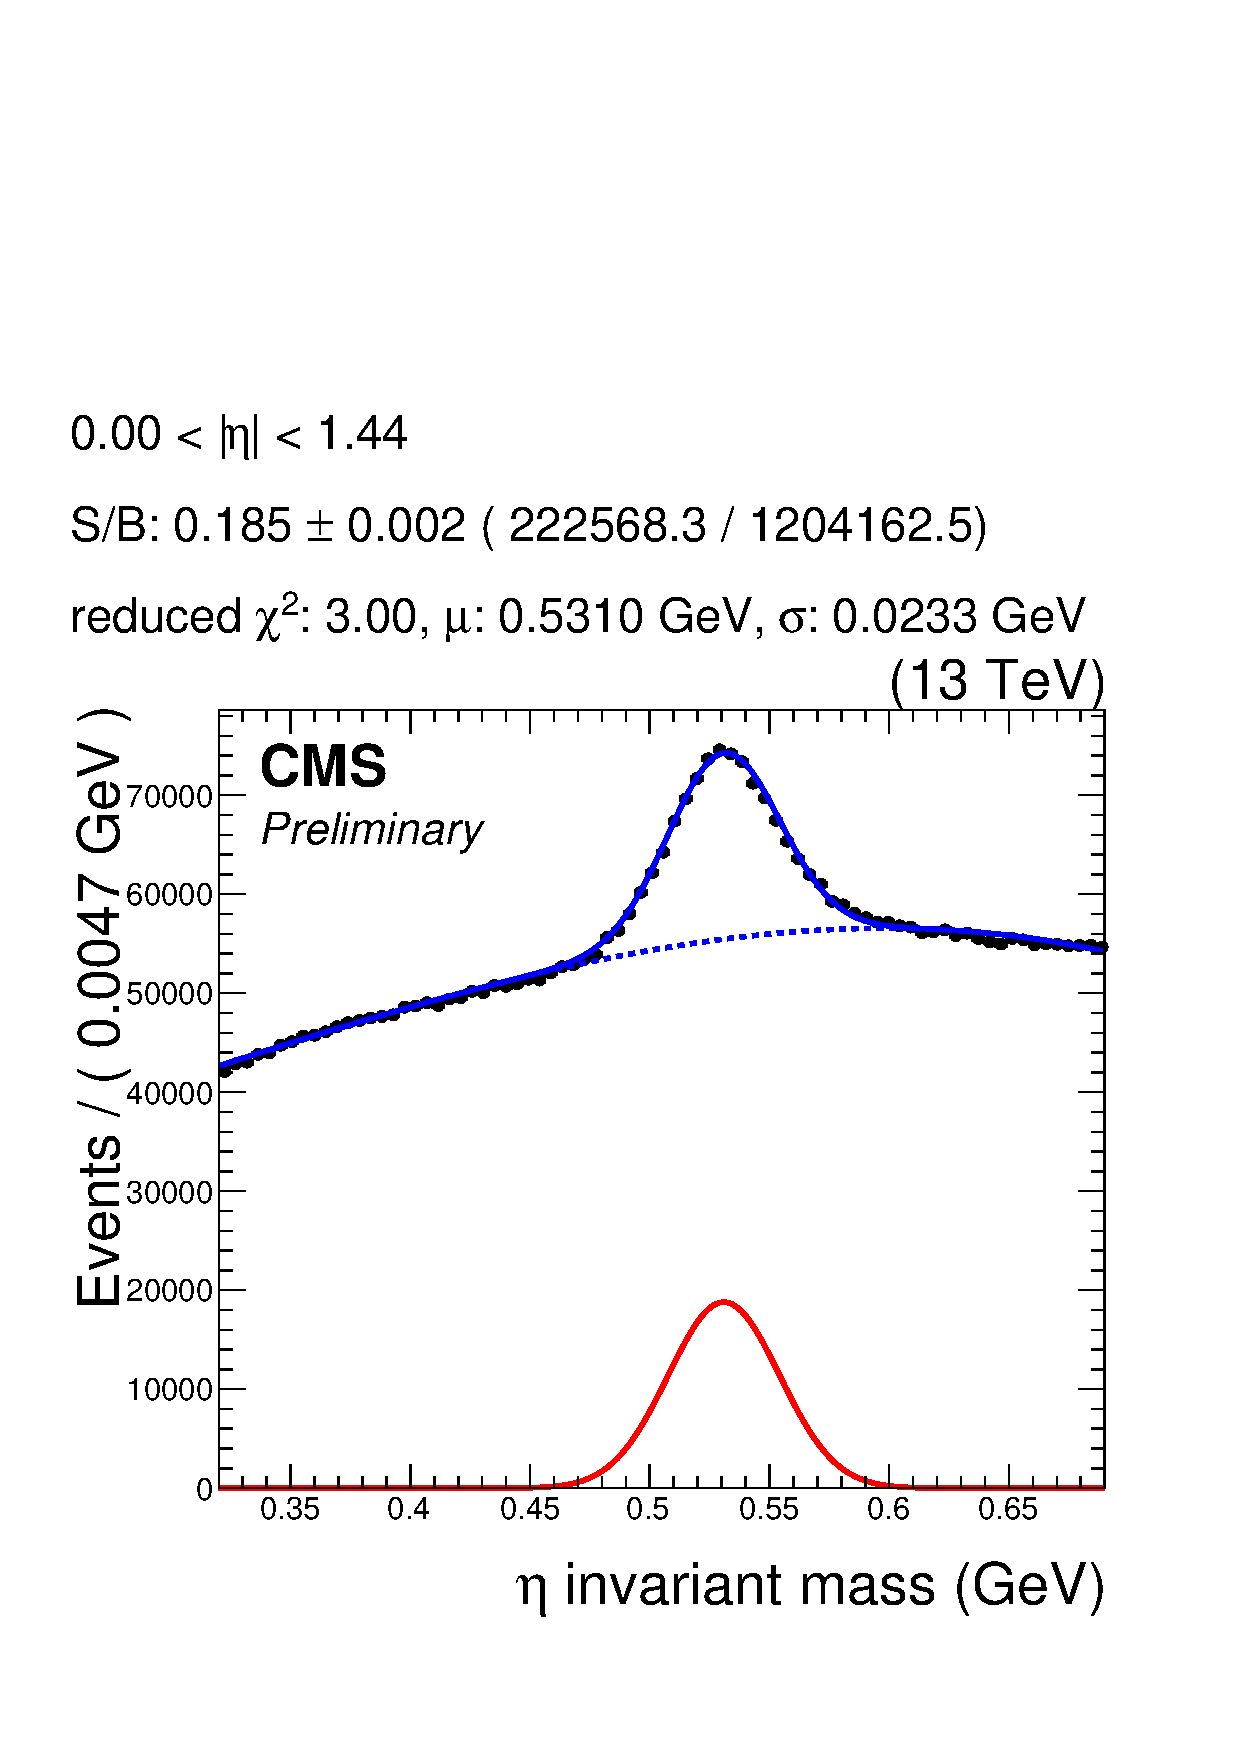
\includegraphics[width=.45\textwidth]{pics/eta_eb_2015b}
\end{center}
\caption{Calibration stream outputs for the pizero and eta barrel trigger paths}
\label{fig:pizero_eta}
\end{figure}

The detector is calibrated with a method that reconstructs the mass of neutral
pion and eta-mesons to precisely calibrate the entire ECAL. The copious
production of these particles in hadronic jets at the LHC allows us to
perform this calibration rapidly, even at very low luminosity.

Under irradiation, the crystals undergo transpancy changes 
due to the formation of color centers, which interestingly recover spontaneously when there
is no radiation present. As the crystal transparency affects the energy measurent,
the crystal transparency is continuoulsy monitored by a laser monitoring system. 
The system takes advantage of a 3 $\mu$s gap in the LHC bunch train to inject the
pulses at a rate of 100 Hz. This rate allows for a measurement of every crystal
to be made at least every 30 minutes. In the barrel, only laser
 pulses of known wavelength are injected through optical fibers. In the endcap, LEDs provide
an additional wavelength. 

The presence of the preshower also causes some degradation of the
Endcaps' energy resolution relative to the Barrel. 



\section{Hadronic Calorimeter (HCAL)}

\begin{figure}
\begin{center}
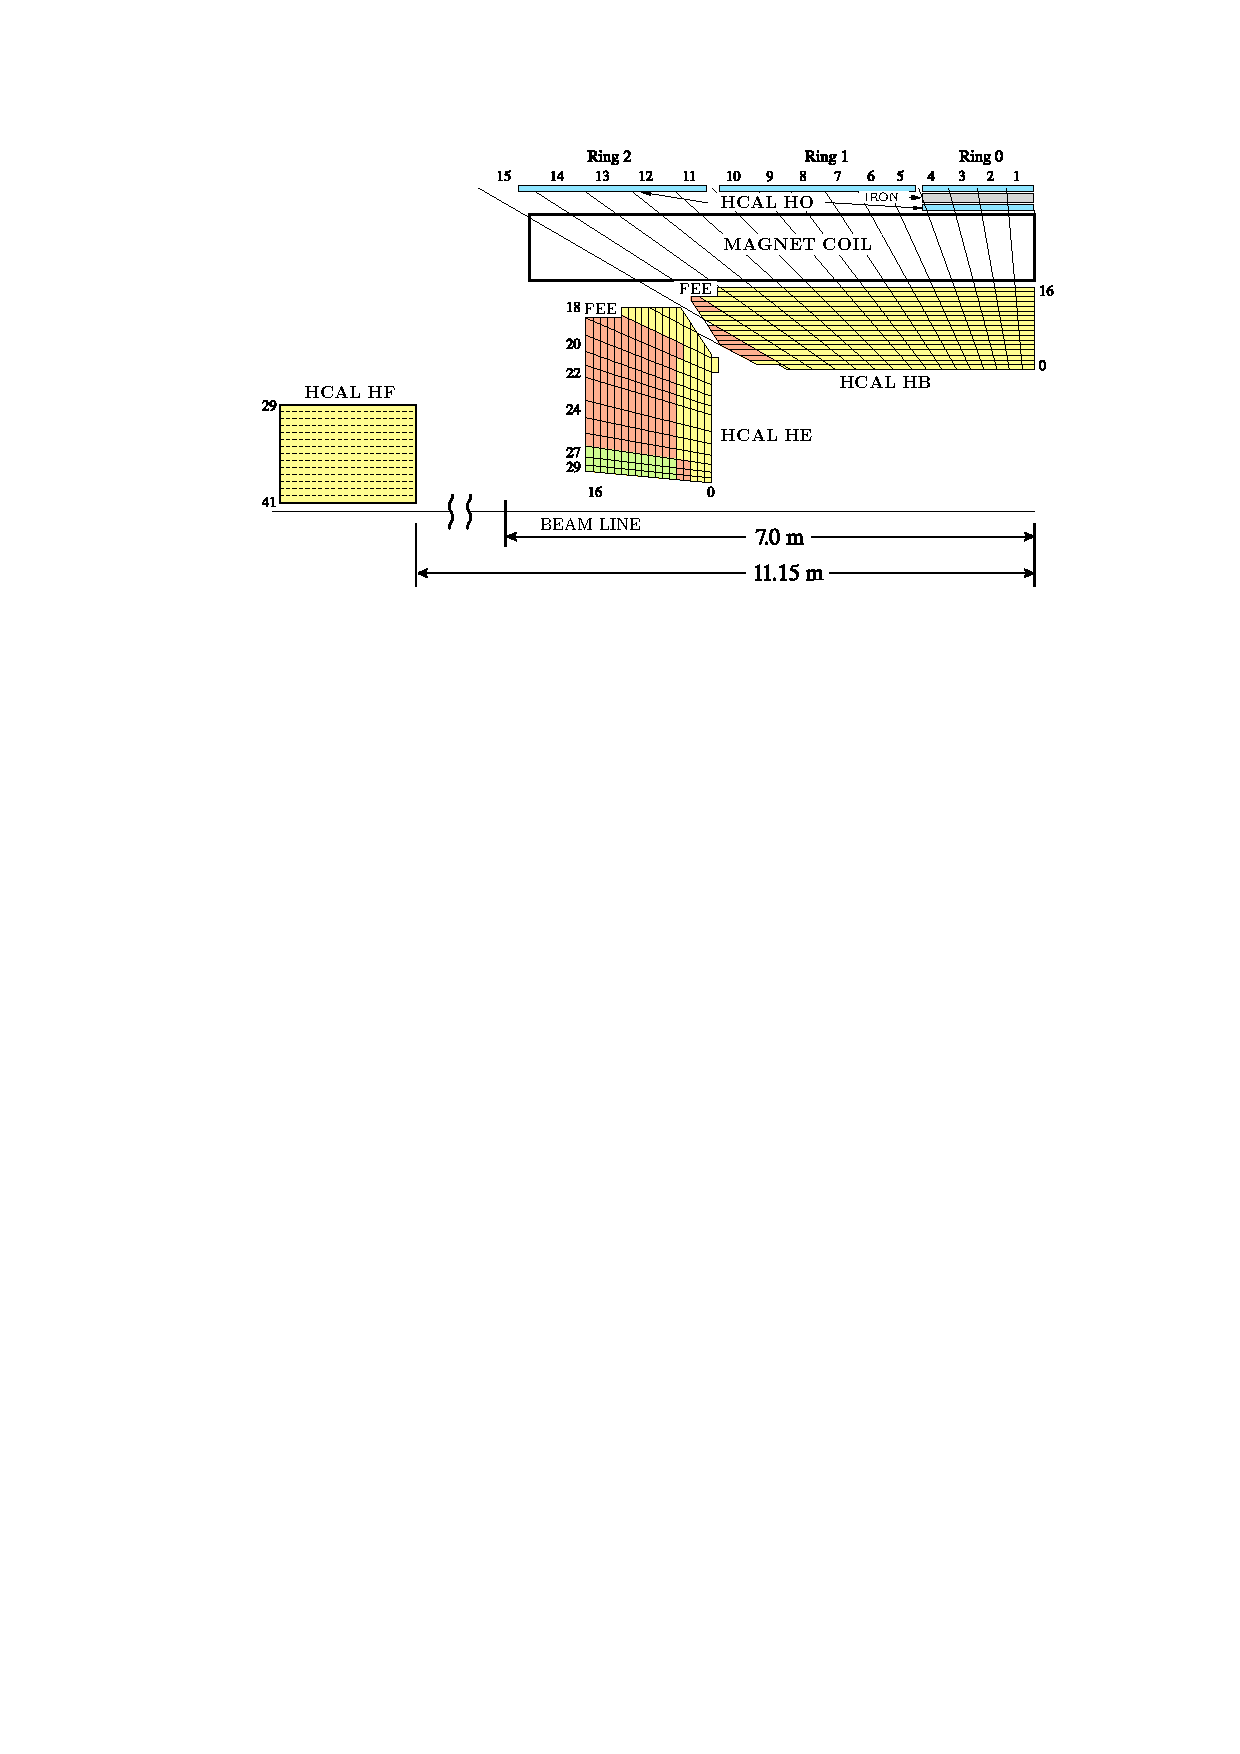
\includegraphics[width=.95\textwidth]{pics/hcal_diagram}
\end{center}
\caption{Kinematic acceptance of the CMS HCAL}
\label{fig:hcal_diagram}
\end{figure}

\begin{figure}
\begin{center}
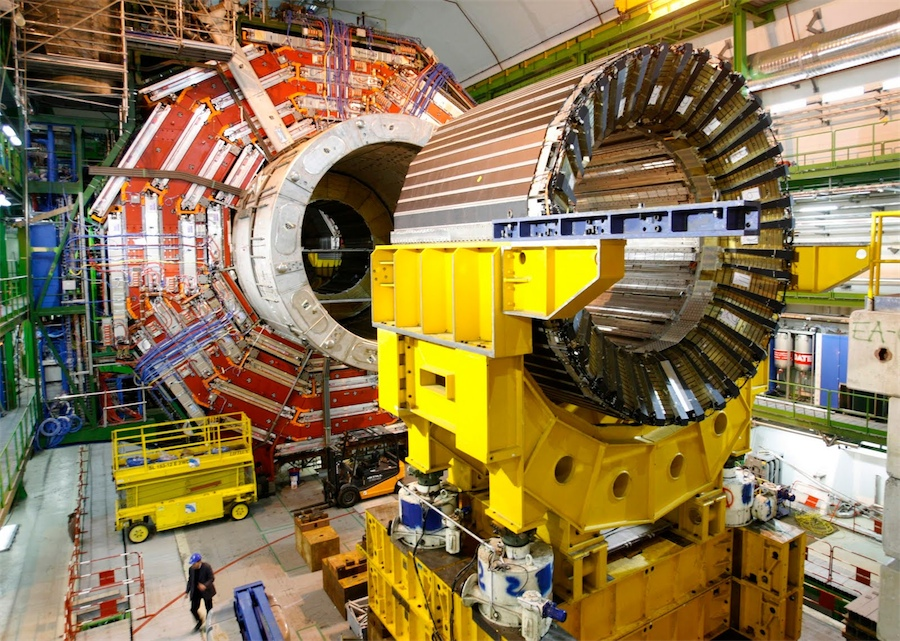
\includegraphics[width=.65\textwidth]{pics/naked_hcal}
\end{center}
\caption{The CMS HCAL outside of the detector}
\label{fig:hcal_naked}
\end{figure}


Surrounding the ECAL. The Hadronic Calorimeter (HCAL) is hermetic (full coverage of interaction), non-compensating (asymmetric eletromagnetic and hadronic energy response), sampling calorimeter (showering material differs from measurment material) designed to measure the the energy of neutral hadrons which would not deposit significant energy in the ECAL. 

 The ratio of energy between the two detectors for defined solid angle, $H/E$, is a 
commonly used particle identification criterion. 

The HCAL consists of 9072 channels divided between four sections: the barrel (HB), the endcap (HE), 
two forward calorimeters (HF) and an outer hadron calorimieter (HO). The barrel
 and endcap of the HCAL cover $|\eta| < 4$. The forward detectors extend the subdetector's reach to $|\eta| =5$. 
As the HCAL is radially limited by the design of the enclosing solenoid, 
the HO is built around the solenoid to measure any leaked energy from high momentum showers. The towers are segmented into towers that project into $\eta,\phi$ space with $\Delta \eta \times\delta \phi= 0.087 \times 0.087$ for $|\eta| < 1.6$ and 
$\Delta \eta \times\delta \phi= 0.17 \times 0.17$ for $|\eta| > 1.6$. 

The HF subdetector is a cherenkov light detector using quartz fibers within 165 cm of steel absorber. 
Photomultiplier tubes (PMTs) connected to the fibers convert the detected light to a detectable signal. Cherenkov detectors
 utilize the characteristic electromagnetic ``sonic boom'' created by particles traveling faster than light can travel in
 a material. As the angle of emission and intensity of the radiation depends on the velocity of the particle. For energetic
particles $E>1$ GeV the energy lost to the radiation is negligble (cite-the-physics-of-particle-detectors-book).

Unlike electromagnetic showers, hadronic interaction cross sections are an order of magnitude smaller for the same material. To compensate cost effectively, hadronic calroimeters are constructed from dense materials usch as copper,
 iron, lead, uranium, and tungsten (cite-tully). In general, hadronic showers produce irregularly 
shaped deposits and varied particle content when compared to electromagnetic showers. 
 
\begin{figure}
\begin{center}
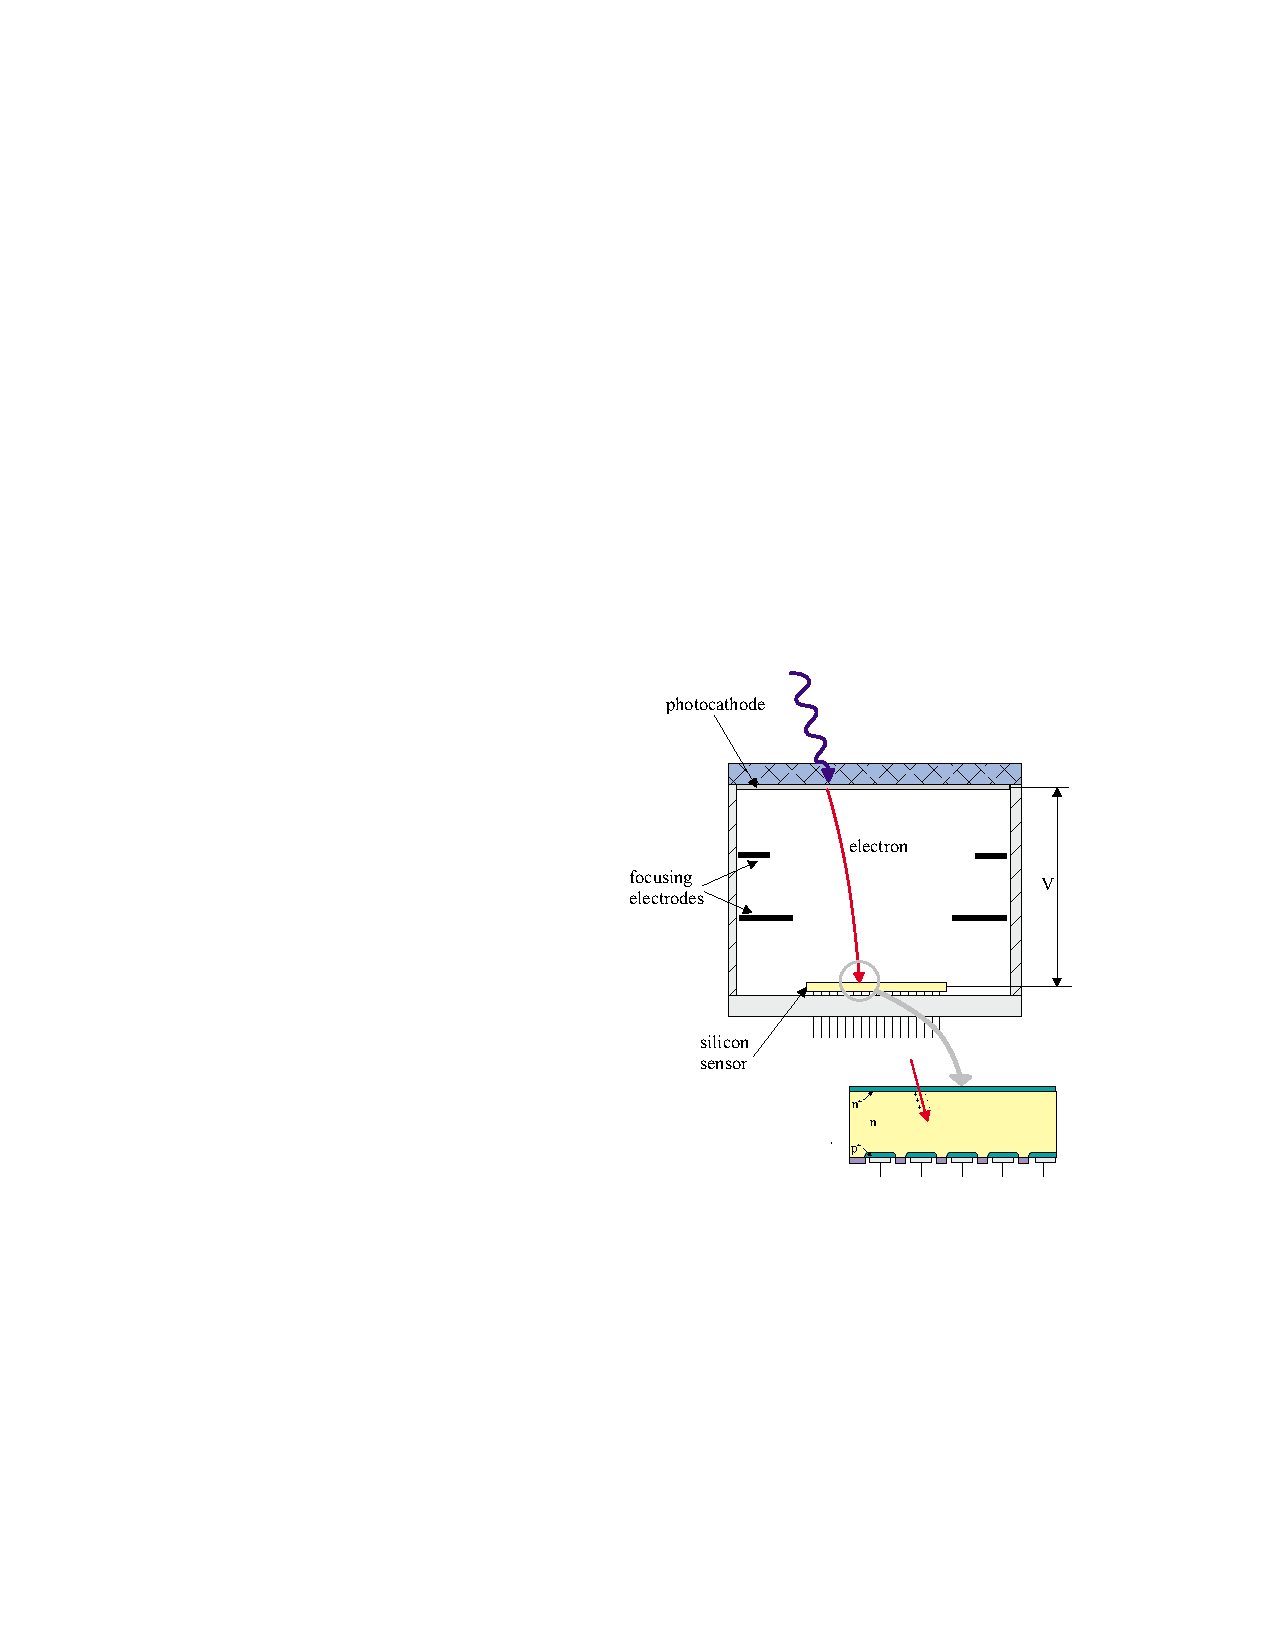
\includegraphics[width=.45\textwidth]{pics/HPD}
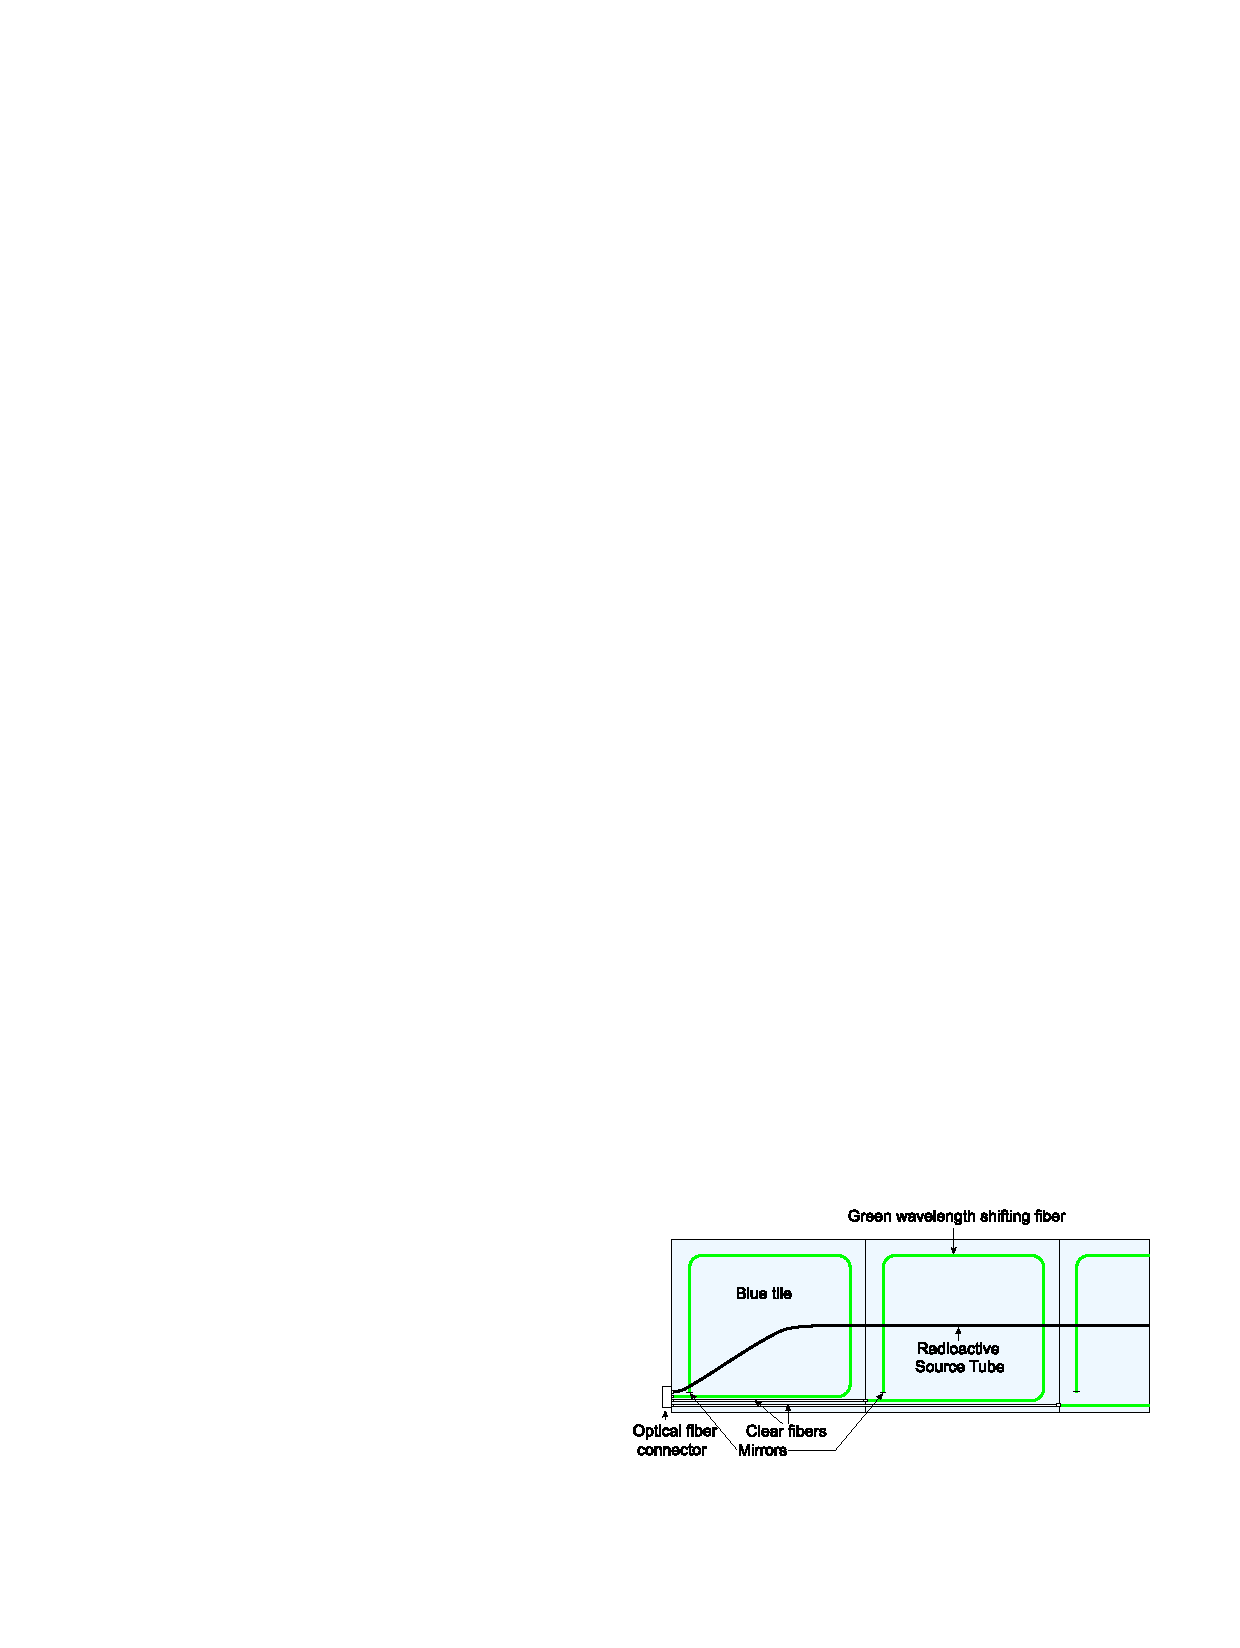
\includegraphics[width=.45\textwidth]{pics/HCALfiber}
\end{center}
\caption{(Left) Diagram of a typical HPD under a potential difference $V$ (cite-hpd-cern) (Right) 2 visible scintillator 
plates of 16 (cite-hcal-calib)}
\label{fig:hpd_fiber}
\end{figure}

\begin{figure}
\begin{center}
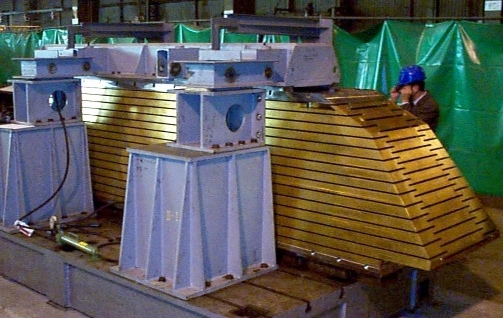
\includegraphics[width=.45\textwidth]{pics/hb_wedge}
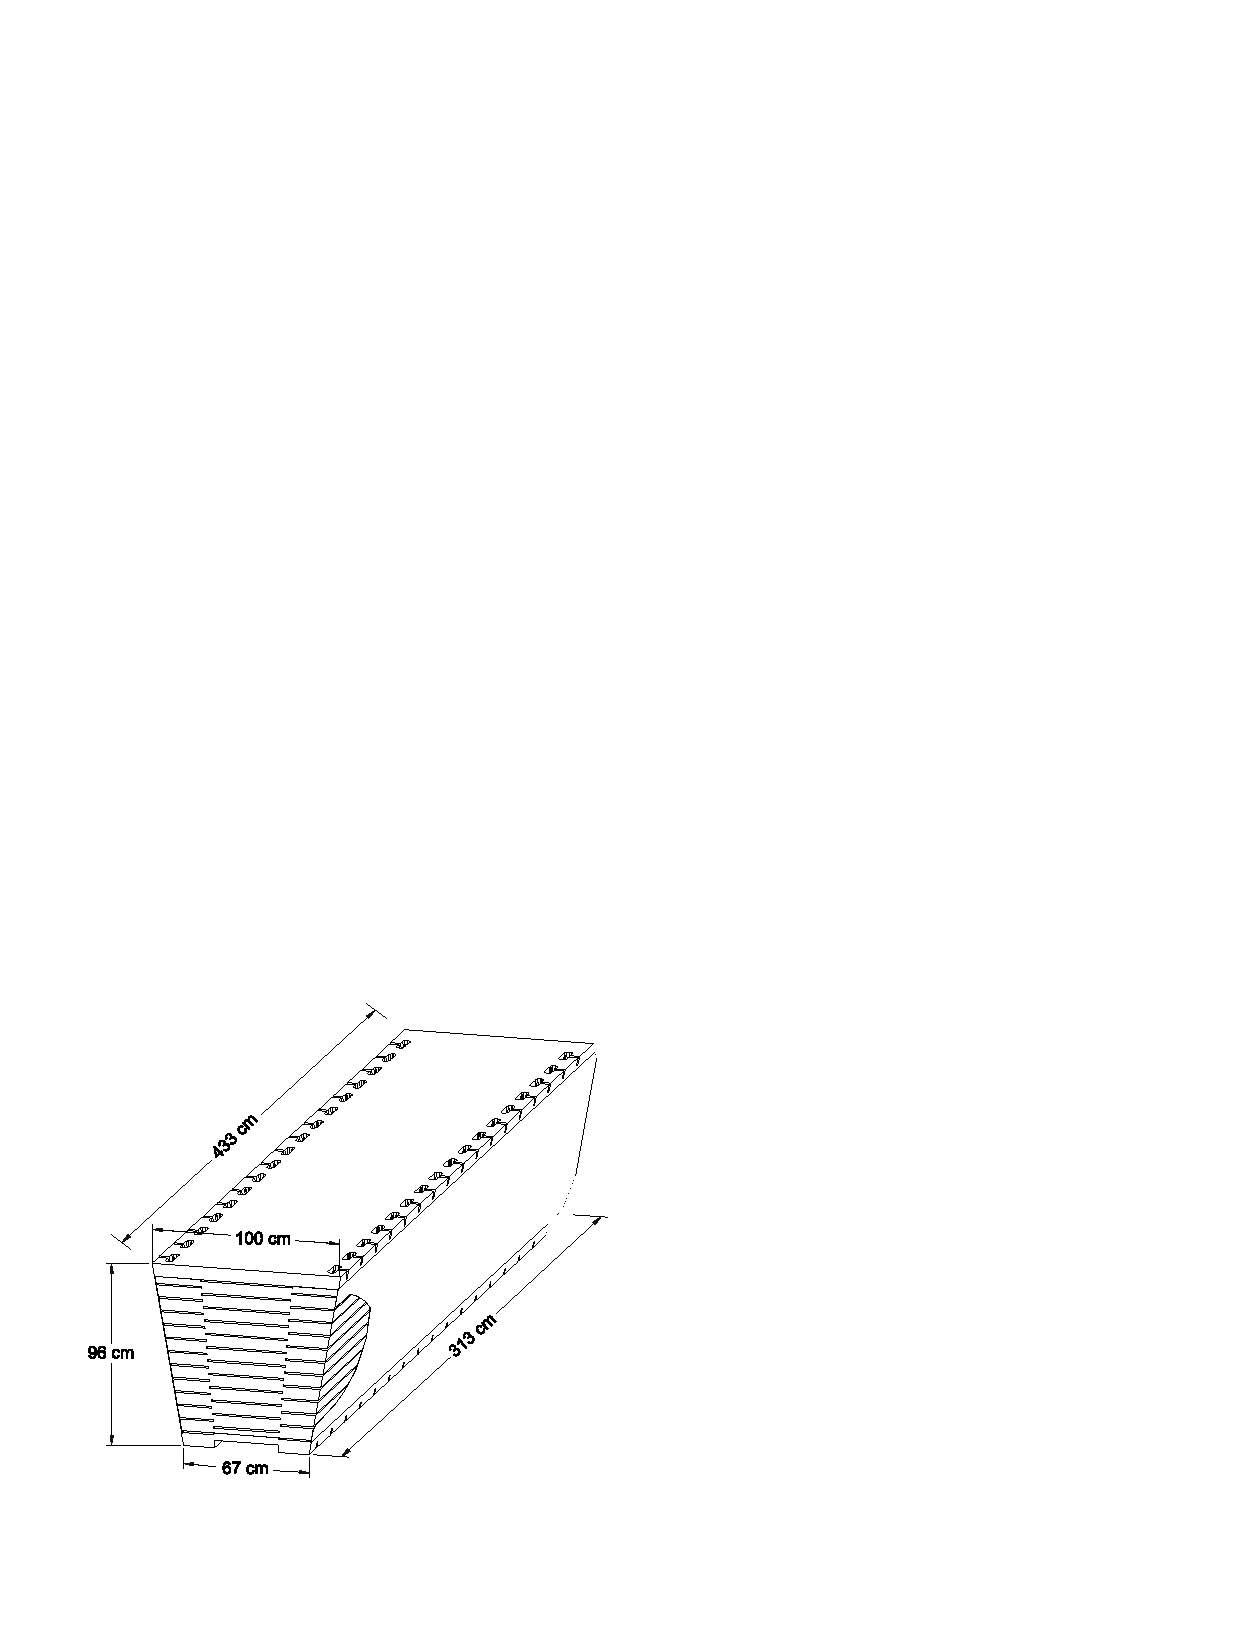
\includegraphics[width=.45\textwidth]{pics/HBwedge}
\end{center}
\caption{(Left) A single wedge of the CMS HCAL barrel (Right) Scintillator trays \ref{fig:hpd_fiber} are inserted into slots at the end of the wedge (cite-hbcalib)}
\label{fig:hb_wedge}
\end{figure}

The detector is constructed as alternating layers of brass absorber and plastic scintillator. 
The light is merged, wavelength shifted and measured by hybrid photodiodes (HPDs) with 17 channels per HPD. The HPD
(Figure \ref{fig:hpd_fiber}) functions by converting light into photoelectrons emitted at the photocathode and accelerated
by a potential difference of 8-10 kV toward the silicon layer. The absorbed energy in the silicon sensor induces 
electron hole pairs which induce a detectable current. The light is wavelength shifted to avoid a loss in photons 
when piping light to the HPDs through a small cross sectional fiber. We are able to evade phase space 
conservation (photon flux per unit area) by redefining the phase space element in a lower energy wavelength specturm.  {

Large deposits of energy reconstructed as purely hadronic energy in the HCAL is of particular interest 
to the study of long lived decays when the long-lived decay occurs inside of the HCAL calorimetetry. Although not studied here,
large signal to background discrimination can be found by requiring a calorimeter deposit to have no
associated tracks and a large ratio of hadronic energy $H/E$. It is also of concern that the HCAL is known to report
 have spurious noise that generally result in the mis-measurement of missing energy, but would mimics the signature
of long lived decays. It is possible that using a coincidence of acitivity in the muon spectromoeter could supressed 
these events.  

\section{Tracking Layers}

\begin{figure}
\begin{center}
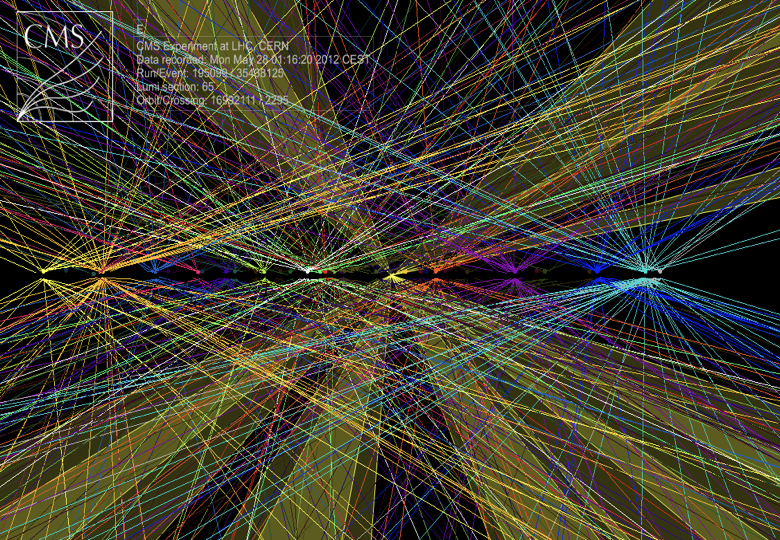
\includegraphics[width=.75\textwidth]{pics/pileup_vertices}
\end{center}
\caption{Pileup Interactions}
\label{fig:pileup}
\end{figure}

The CMS tracker's purpose is to reconstruct the trajectories (or simply ``tracks'') of the charged particles
 copiously produced in hadron collisions. Using knowledge of the magnetic field along trajectory
 with position measurements taken from multiple layers of silicon strips and pixels, the helicoidal tracks are
 fit and kinematic parameters extracted.  

A charged particle in a uniform magnetic field (like that of the CMS Solenoid) 
are parameterized by 5 parameters:
\begin{itemize}
\item $d_{\rho}$: the distance of closest approach to the reference point
\item $\phi_0$: azimuthal angle specifying the reference point to the helix center 
\item  $p_t^*$: charged signed transverse momentum
\item  $d_z$: signed distance of the helix from the reference point in the z direction
\item $\tan \lambda$: the slope of the track 
\end{itemize}
using these parameters, the trajectory is parameterized in the turning angle $\phi$:
\begin{align*}
x =& x_0 + d_\rho \cos \phi_0 + \alpha p_{t}^* ( \cos \phi_0 - \cos(\phi_0 + \phi) ) \\
y =& y_0 + d_\rho \sin \phi_0 + \alpha p_{t}^* ( \sin \phi_0 - \sin(\phi_0 + \phi) ) \\
z =& z_0 + d_z - \alpha p_{t}^*  \tan \lambda \cdot \phi 
\end{align*}
It is important to note that tracks do not necessarily  have the same reference point. For CMS, each
individual track parameter is computed against a reference point determined by the the closest
point of approach to the beamline. For prompt physics, this reference point coincides with the
collision vertex used to compute the kinematic parameters for calorimeter jets. In contrast, when
tracks are displaced, the reference point used for the track is not the same as the reference point
for the calorimeter jet $eta$ and $\phi$. This mis-match of coordinate systems affects the ultimate
track and jet association. 

By fitting trajectories to vertices the tracker enables the reconstruction 
of the hard interaction position (Figure \ref{fig:pileup}). As only one vertex is typically
of interest, identifying background vertices and subtracting their contribution is of increasing
importance with the increasing instantaneous luminosity. 

As photons and electrons exhibit nearly identical signatures in the ECAL, the reconstruction of the
track associated to electrons is of particular interest.

\begin{figure}
\begin{center}
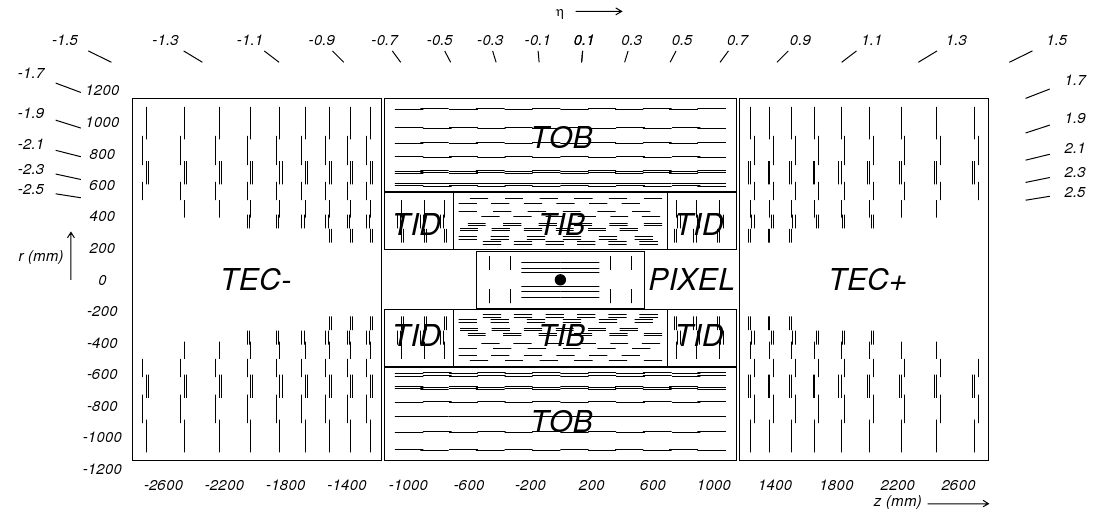
\includegraphics[width=.95\textwidth]{pics/tracker_diagram}
\end{center}
\caption{Kinematic acceptance of the CMS tracker}
\label{fig:tracker_diagram}
\end{figure}

The CMS tracker is the worlds largest all silicon detector with a
 sensitive area larger than 200 m$^{2}$ (Figure \ref{fig:tracker_strips_and_module}) (cite-2014-tracker-performance). 
The tracker consists of 10 layers
in the barrel region: 4 inner barrel layers (TIB) and 6 outer barrel layers (TOB). The endcap is made up of 
12 disks: 3 inner disks (TID) and 9 endcap disks (TEC). 


\begin{figure}
\begin{center}
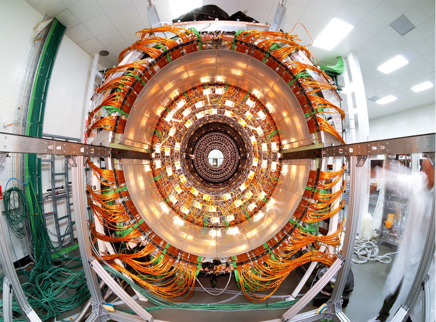
\includegraphics[width=.45\textwidth]{pics/naked_pixel}
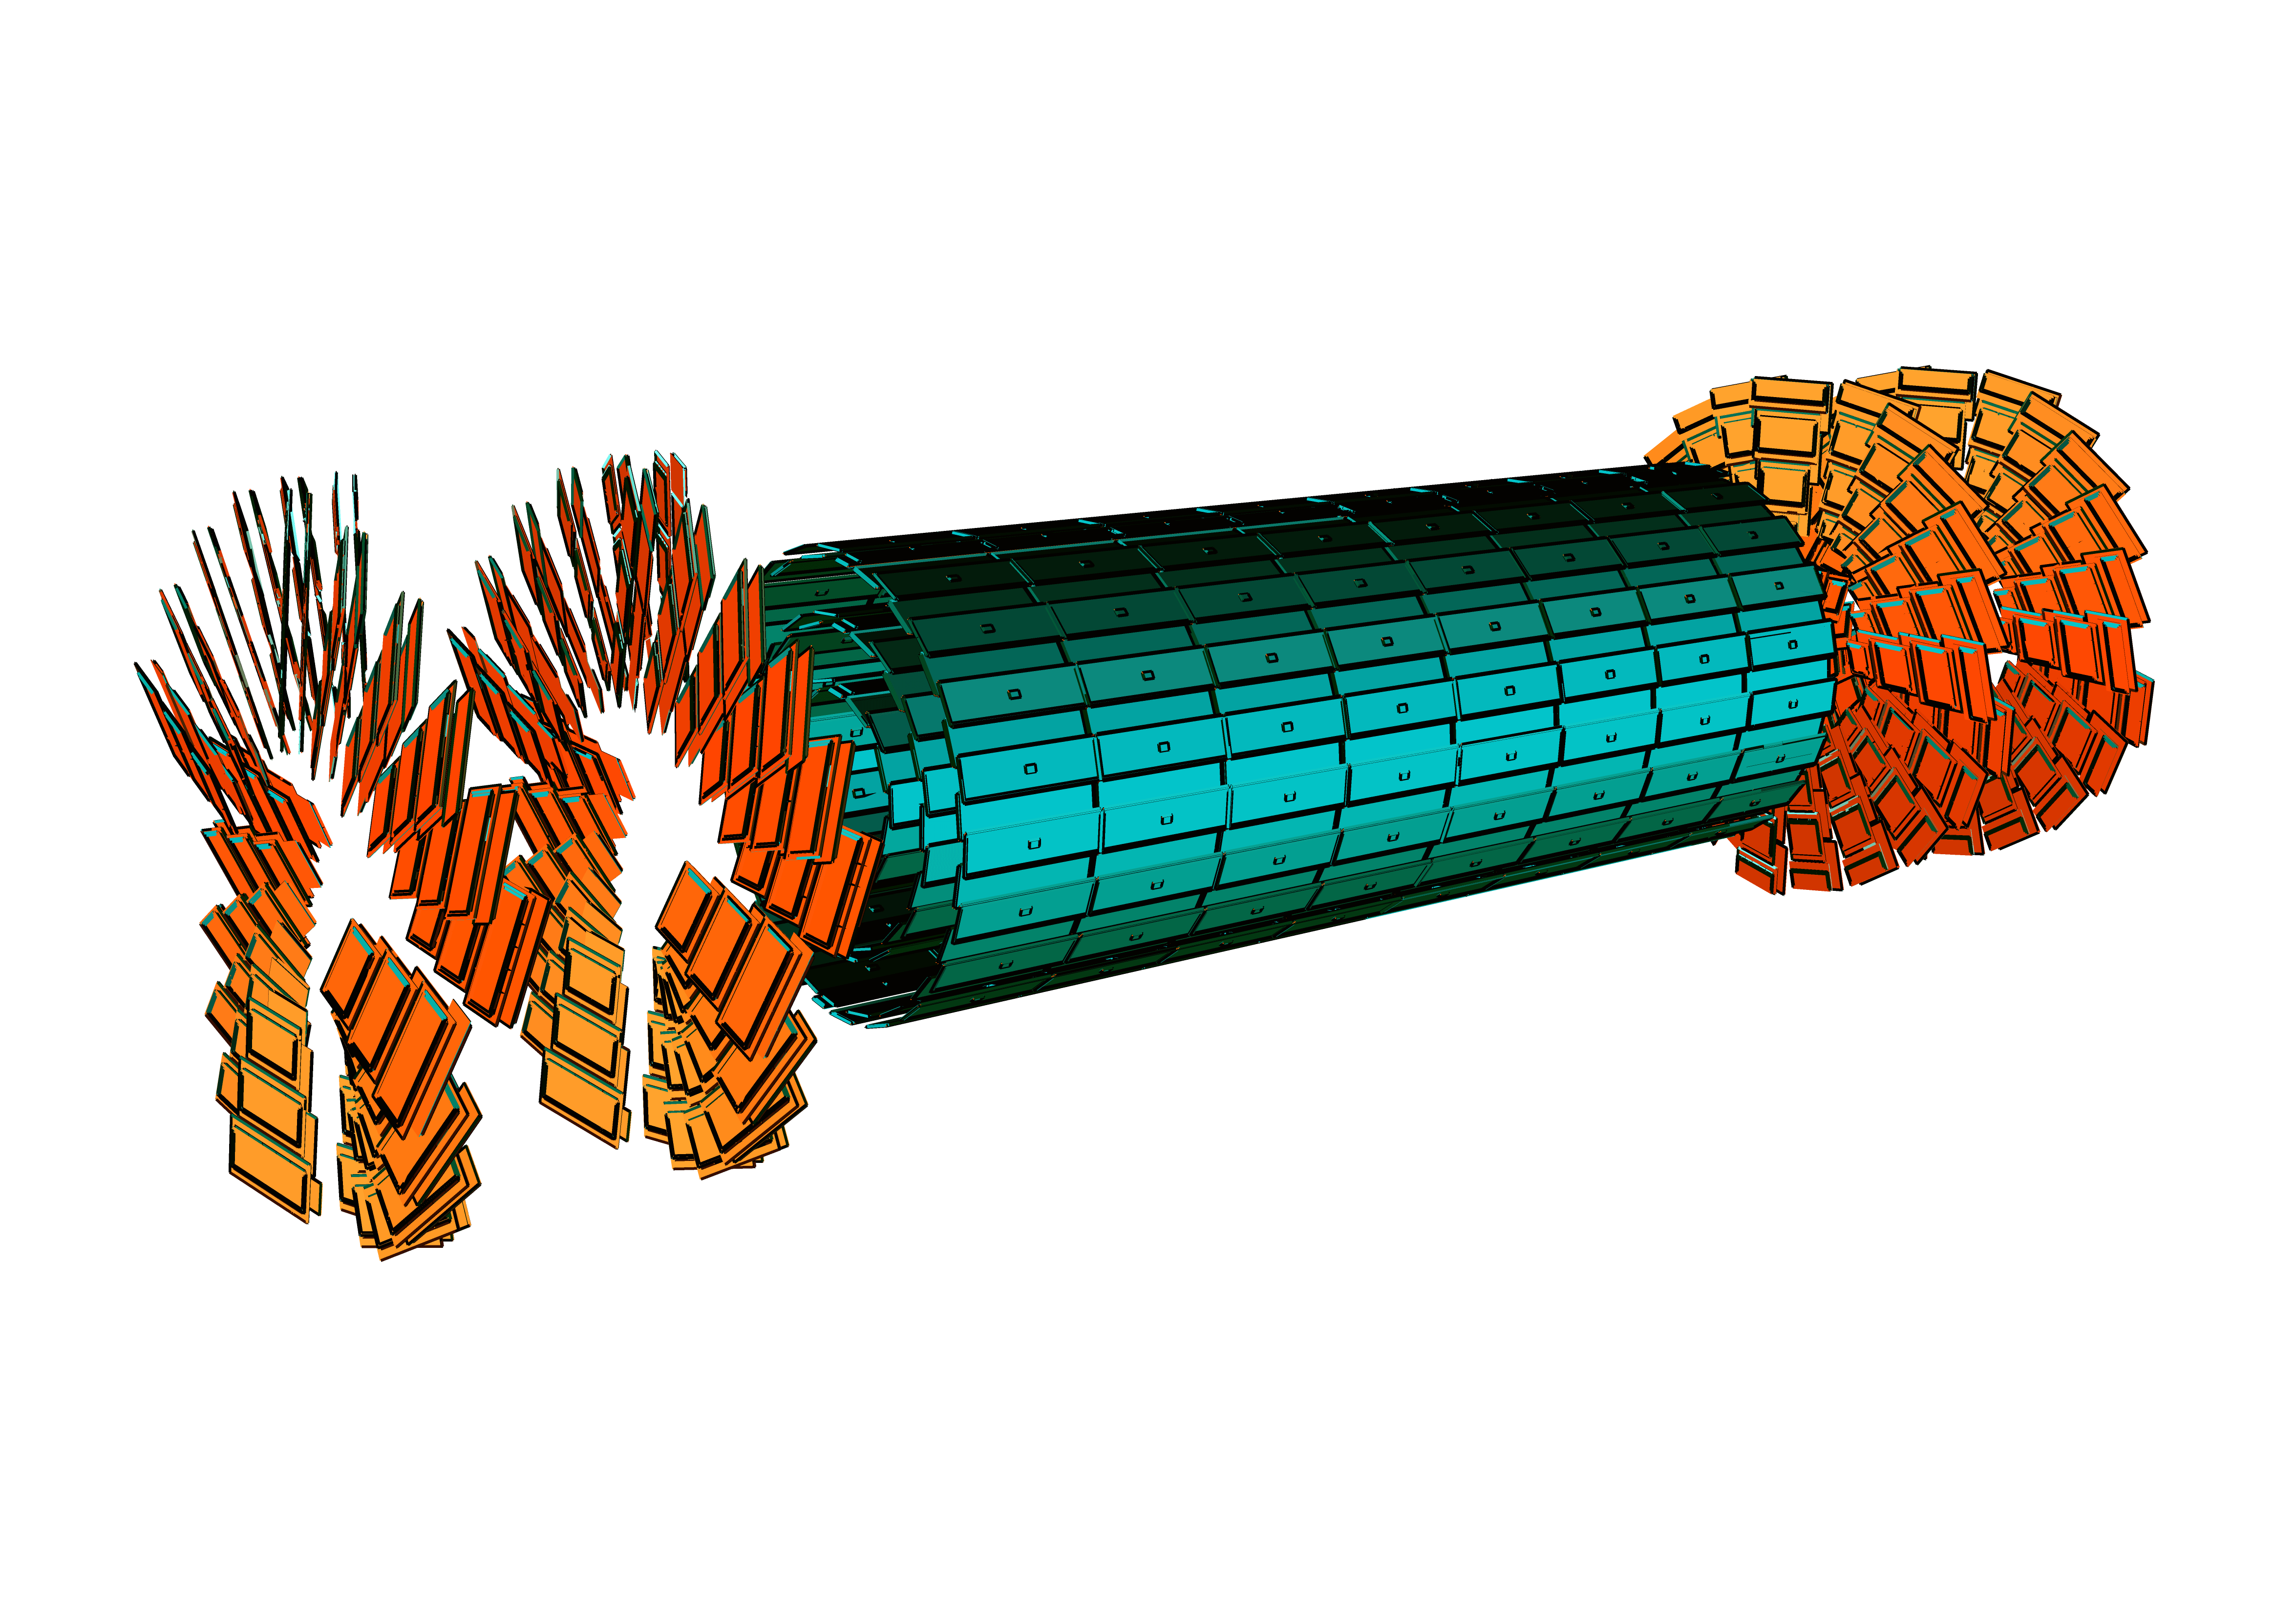
\includegraphics[width=.45\textwidth]{pics/pixel_diagram}
\end{center}
\caption{The CMS Pixel detector }
\label{fig:pixel}
\end{figure}

The CMS pixel detector (Figure \ref{fig:pixel}) consists of three layers are radii of 5.3 cm, 7.2 cm and 11 cm and 2 disks on each size of the barrel at 34.6 and 46.6 cm from the either side of the interaction point. 

\begin{figure}
\begin{center}
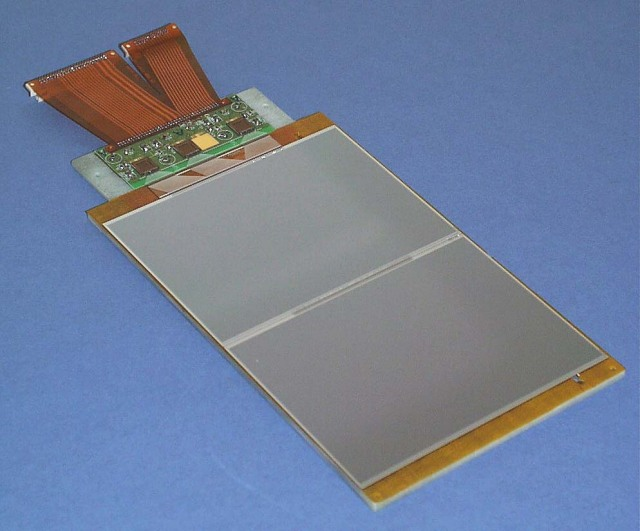
\includegraphics[width=.45\textwidth]{pics/tracker_module}
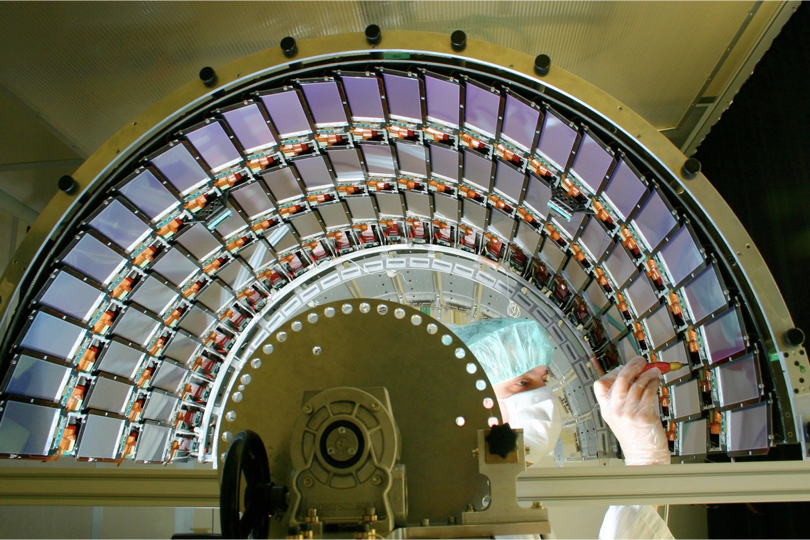
\includegraphics[width=.45\textwidth]{pics/tracker_strips}
\end{center}
\caption{A single CMS tracker module (left) and a tracker inner barrel module (right)}
\label{fig:tracker_strips_and_module}
\end{figure}

Track reconstruction is degraded by the interaction with the tracker material. With some finite probability
as a function of the material density and thickness, the track with randomly scatter. 

High energy charged particles for which the detector volume and strength of the magnetic field do not permit the track
to bend cause significant degregdation of momentum resolution as well as charge sign detrmination. For low energy tracks, 
the magnetic field 

\section{Muon Spectrometer}

\begin{figure}
\begin{center}
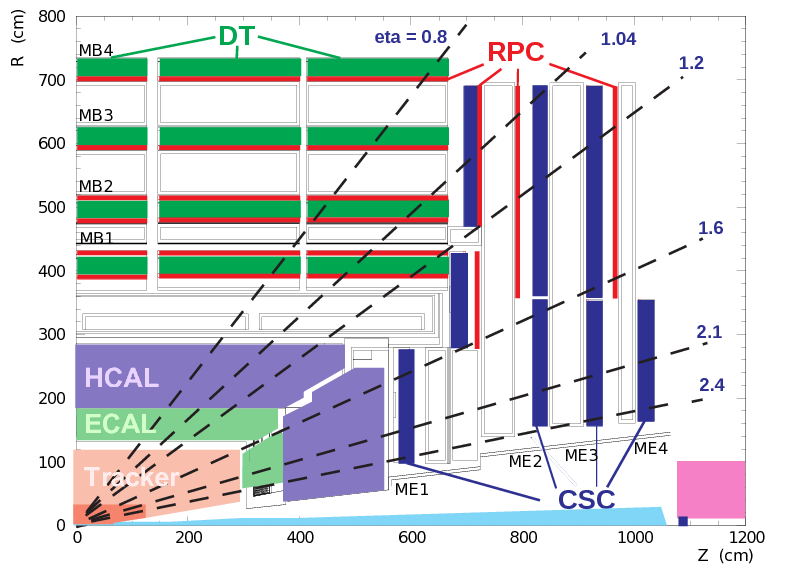
\includegraphics[width=.85\textwidth]{pics/muon_diagram}
\end{center}
\caption{Kinematic acceptance of the CMS Muon System}
\label{fig:muon_diagram}
\end{figure}

\begin{figure}
\begin{center}
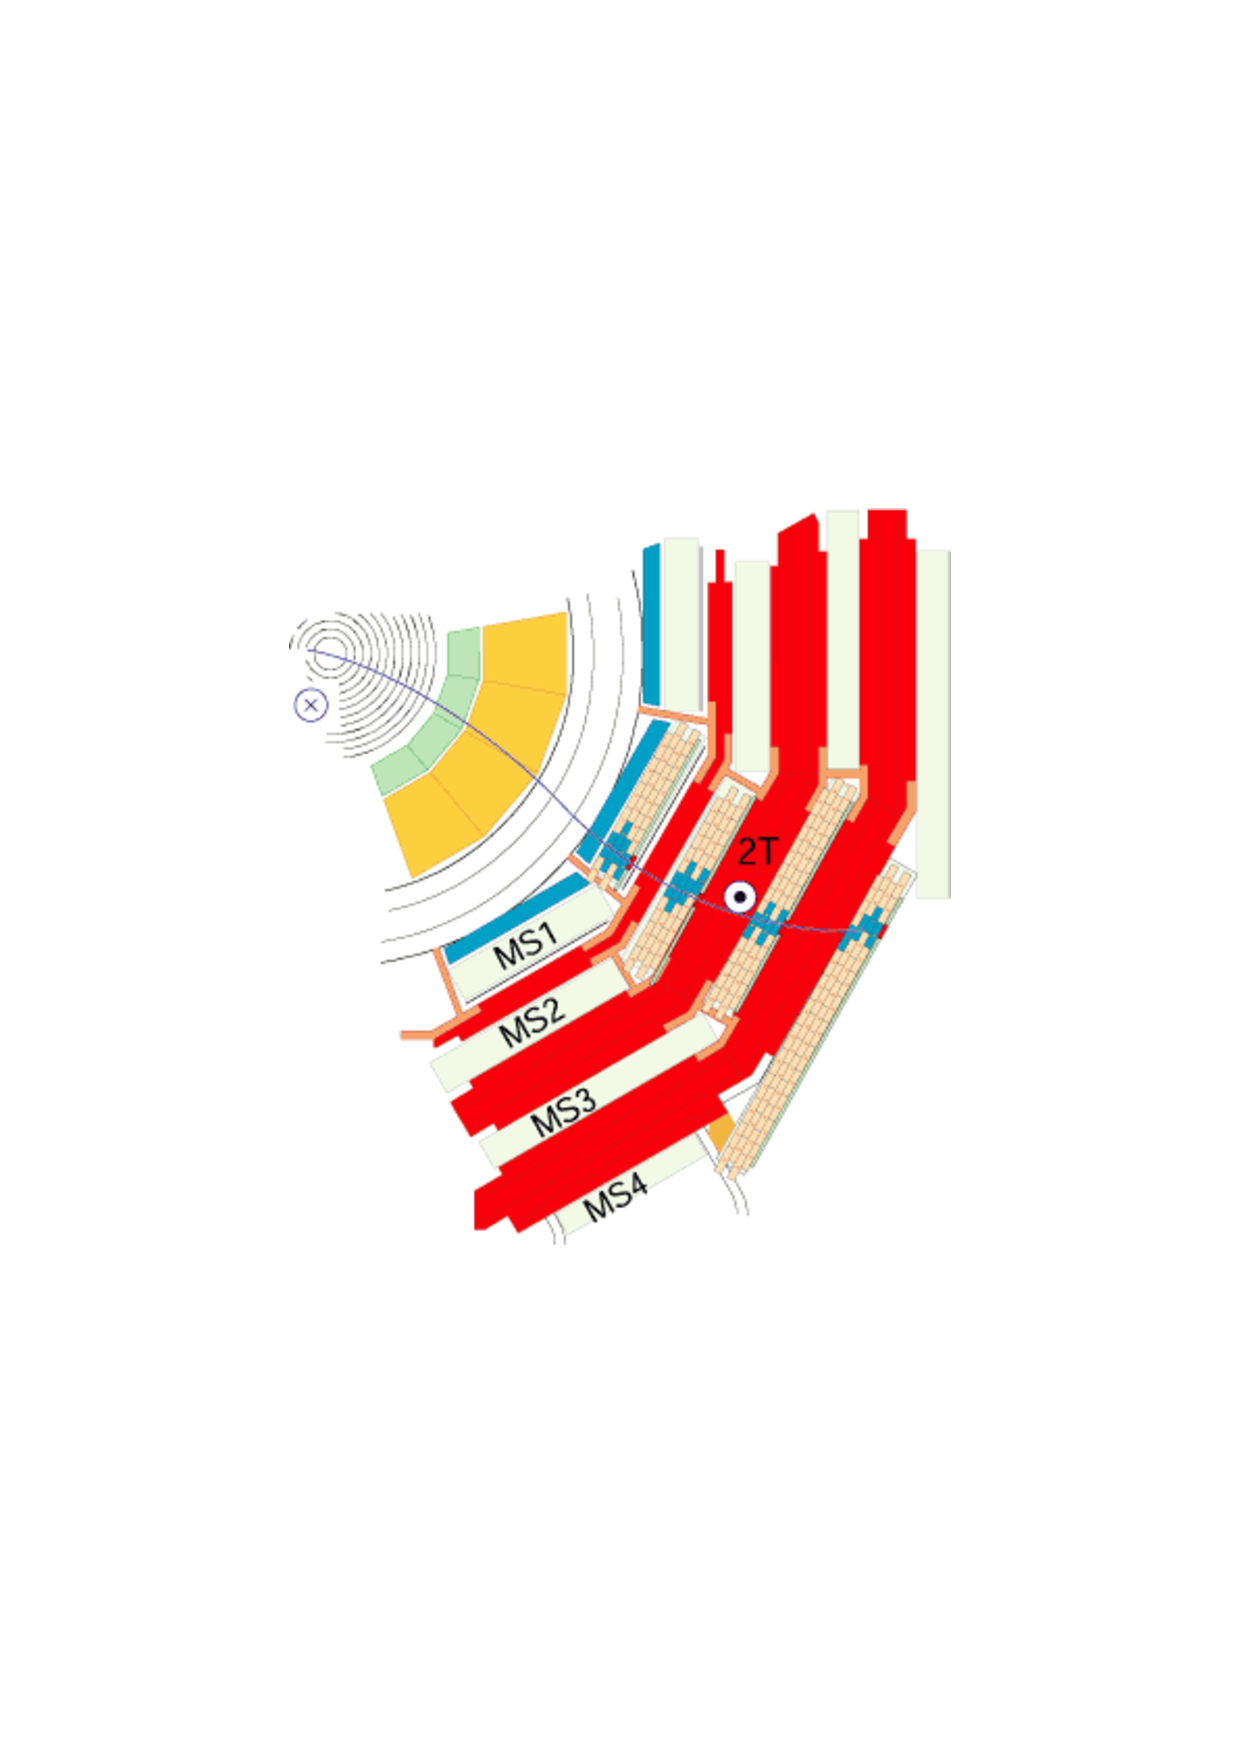
\includegraphics[width=.45\textwidth]{pics/muon_slice}
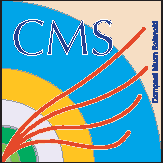
\includegraphics[width=.45\textwidth]{pics/cms_logo}
\end{center}
\caption{Slice of the muon detector (left) and cms logo (right)}
\label{fig:muon_slice}
\end{figure}


\begin{figure}
\begin{center}
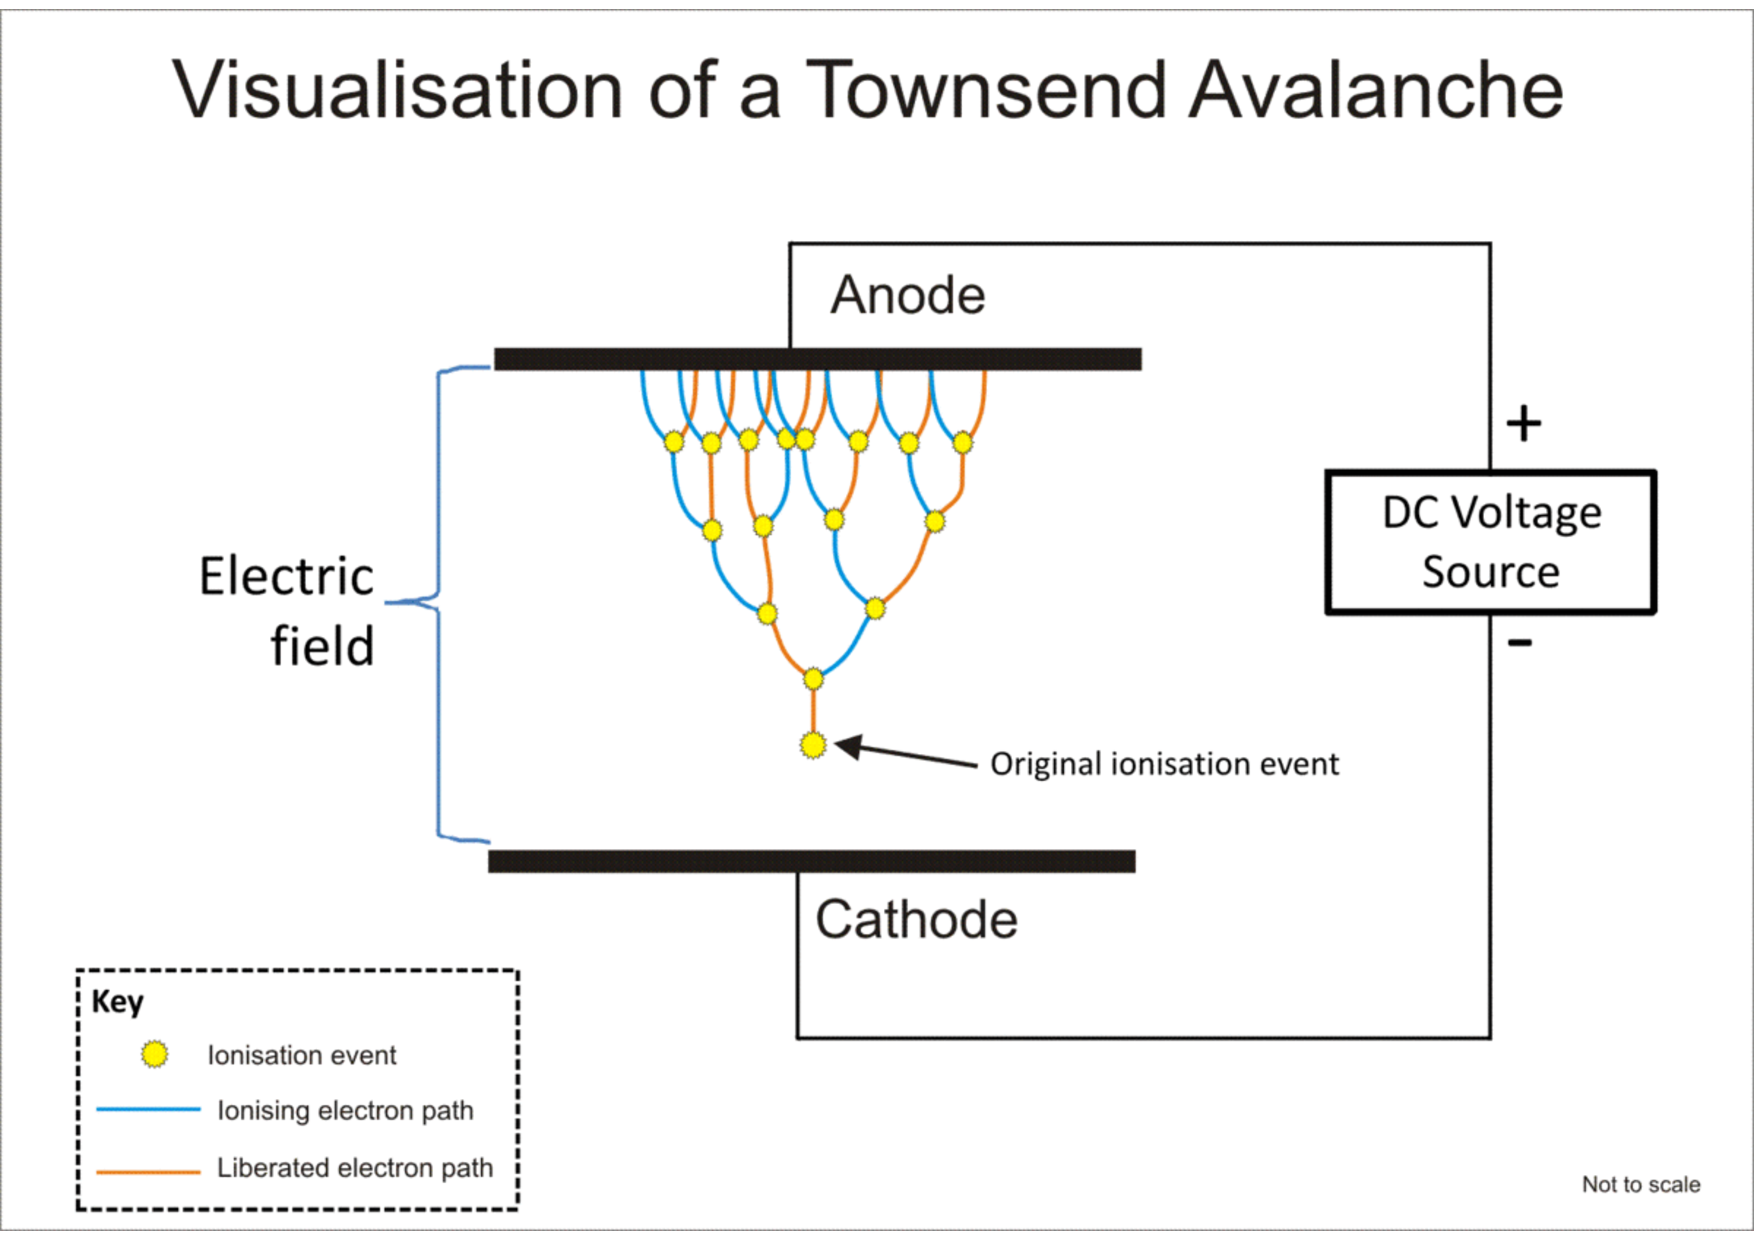
\includegraphics[width=.45\textwidth]{pics/avalanche}
\includegraphics[width=.45\textwidth]{pics/cell_diagram}
\end{center}
\caption{When a gaseous medium is ionized by the track of a muon the resulting liberated electrons are accelerated
in the electric field and collide with gas molecules. The result is an avalanche of electrons collected at the anode. 
The processes is known as a Townsend Avalanche (left) The drift tube design showing the drift lines.  }
\label{fig:avalance}
\end{figure}

The Compact Muon Solenoid's name is partly taken from the Muon subsystem which is
 built to identify and measure the trajectories of muons. The search for displaced jets uses only calorimeter
quantities and inner tracking correspondingly no sensitivity to muons and no muon vetos.
 This section is included only for completeness.  

The muon system consists of 3 separate detectors: drift tubes (DT's), resistive plate chambers (RPCs), and 
cathode strip chambers (CSCs). All three systems rely on the ionization of a gas medium caused by the charged muon's
traversal through the detector. The detectors are multi-layered and sandwiched betwen between layers of the iron  return
yoke (Figure \ref{fig:muon_diagram}). The iron layers aid in particle identification by stopping nearlly all
 other particle activity before the final detector layer. As  muons are very weakly interacting, they should be the only
particles reaching the edge of the detector. When the magnetic field changes outside of the solenoid, muon tracks
will change curvature in the muon system as depicted in the CMS logo (Figure \ref{fig:muon_slice}). The second measurement
made in the muon spectrometer improves the momentum resolution for energetic muons $>100 GeV$, however lower momentum muons are dominanted by a increase of multiple scattering from the additional detector material. 

It the context of long-lived searches it is interesting that the muon is the only long-lived fundamental particle, with
 a finite lifetime of $\tau_0=2.2 \mu$s or equivalently $c\tau_0 = $ 660m. The dominant decay to an electron and two neutrinos  is suppressed by requiring the muon decay with an  offshell decay through the much heavier $W$. 
This method of generating long-lived signatures mirrors the motivations of
split supersymmetry where the gluinos are long-lived as they must decay through much heavier squarks.
If this were the end of the story we would expect $\approx$ 1\% of muon decays to occur before the final layer.  However, a moderately energetic muon will experience time dilation $c\gamma\tau_0$ in the lab frame with 
$\gamma = E / m = (1$ GeV$)/ 105$ MeV $\approx 10$. Accordingly, on detector length scales $O(10$ m$)$ energetic muons can be considered stable. 

The drift tube system located in the barrel region covers $|\eta| < 1.2$ with 4 concentric rings (segmented in $r=4.0,4.9,5.9,7.0$ m) referred to as ``stations''. Five divisions are also made in 
the $z$ direction referred to as ``wheels'' partitioned into 12 sectors of 30 degrees.  The three inner cylinders have 
60 chambers each and the outer cylinder has 70.   Each chamber measures 3.0m x 2.5m.
 Each chamber is divided into 3 (or 2) super layers with 4 drift cells per layer (2 in $\phi$, 2 in $z$). The drift cells
use  anode wires at voltage of $+3.6$ kV, electrode strips at 1.8kV and -1.2kV cathode strips  to detect the localized ionization showers from muon tracks (Figure \ref{fig:avalanche}). The full system includes 172,000 wires.  The maximal path of drift is 21 mm corresponding 
to a drift time of 380ns in a gas mixture of 85\% Argon and 15 \% CO$_2$. (cite-complete-cms-description)

The CSCs and DTs are  located in the endcap region. The CSCs are located between $0.9 < |\eta| < 2.4$ and the RPCs between $0.9 < |\eta| < 1.6$. There are 4 stations for each endcap. The CSCs are trapezoidal multiwire proportional chambers comprised
 of 6 wire planes interleaved with 7 cathode panels. The chambers extend 1.7 (or 3.4) m 
in the radial direction covering 10 or 20 degrees. Each chamber layer 
Wires running in the $\phi$ direction define a tracks radial position. The $\phi$ 
coordinate along the wires is obtained by interpolating charges induced 
on the cathode strips. 


\begin{figure}
\begin{center}
\includegraphics[width=.45\textwidth]{pics/cathode_strip_chamber}
\includegraphics[width=.45\textwidth]{pics/rpc_plates}
\end{center}
\caption{The Muon Cathode Strip Chamber}
\label{fig:strip_chamber}
\end{figure}


\section{Trigger System}

\begin{figure}
\begin{center}
\includegraphics[width=.95\textwidth]{pics/counting_room}
\caption{Location of the counting room relative to the experimental hall}
\end{center}
\label{fig:counting_room}
\end{figure}

\begin{figure}
\begin{center}
\includegraphics[width=.5\textwidth]{figures/exp_proj/pdf_xsec.png}
\caption{Common cross sections of proton collisions as a function of the center of mass energy $\sqrt{s}$}
\end{center}
\label{fig:pdf_xsec}
\end{figure}

The CMS Trigger System exists as a filter through which events are determined to be interesting or 
useful enough to be written down. The name comes from the nature of algorithms used to determine 
what to write down. If an event passes any of the online algorithms, this ``triggers'' the collision to be 
written down in its entirety regardless of the goals of the path in particular 
 (albiet with some notable exceptions). It is both  unnecessary and impractical to record every
collision the LHC delivers. The low momentum transfser  hadronic events contained in the vast majority of
 proton collisions is well understood from past experiments. Figure \ref{fig:pdf_xsec}  shows 
typical physics processes for proton-proton scattering. Events such as the production 
of a $b$ quark  occur at $\approx 10^6$ Hz at a luminosity of $\mathcal{L} = 10^{33}$ cm$^{-2}$ 
whereas processes of interset, such as the production of the Higgs is much lower at $\approx 10^{-2}$ Hz.  

The LHC has beam crossings at a rate of $\approx 40$ MHz with 
each crossing coming spaced at $\approx$ 25 ns. The number of ineleastic collisions per bunch cross crossing
 is given by the  is the total inelastic cross section times the luminosity divided by the bunch collsion rate. 
This is respectively $8.5\times 10^{-26}\text{cm}^2 \times 10^{34}\text{cm}^{-2}\text{s}^{-1}/ (40 \times 10^6 \text{s}^{-1} \approx 24$ (cite:arXiv:1204.5689). 
The collisions are stored with an average file size 1 MB in their unprocessed form in a format refered to as \texttt{RAW}. However the bandwidth for the combined constraints of
 aquisition rate, storage and processing, is limited to $10^3$ Hz and equivalently $10^3$ MB/s. 
Generally, all but one of the inelastic collisions is interesting and a large excess of  
activity is generated in the detector electronics. The trigger must be robust enough to select 
these events efficiently while remaining  efficient in maximizing the limited bandwidth.  

\begin{figure}
\begin{center}
\includegraphics[width=.4\textwidth]{figures/exp_proj/cms-trigger}\\
\caption{A diagrammatic representation of the level 1 and HLT trigger processing (cite-tridas-tdr)}
\label{fig:l1_hlt_diagram}
\end{center}
\end{figure}

The CMS Trigger system is designed to read events at the event crossing frequency and generate the
 factor $10^5$ of rejection between the crossing frequency and the archival capacity. This factor 
is too large to achieve in a single step given the complexity of triggers and event reconstruction necessary
to build efficient algorithms. Therefore the task is split into two steps The Level 1 (L1) and High Level
 (HLT) Trigger systems (Figure \ref{fig:l1_hlt_diagram}). The L1 system is a coarse study of an event designed
 to be fast and capable of analyzing every event at 40 MHz. The HLT provides the flexibility the L1 lacks 
permitting as much event reconstruction 

%% The $O(10^7$) events per second first pass through the L1 Trigger which reads out events at $10^5$ Hz. 
%% From here, the High Level Trigger makes the final decision as to which events are kept. 
%% Approximately 350 Hz is processed and stored, 300 Hz is ``parked'' (stored but processed later), 
%% and 1 kHz is partially stored (only the HLT level information and not the RAW detector information) 
%% and used for data scouting for future analysis.  

The most obvious criterion for interesting events are hard physics events with high momentum transfer, $q^2$, and
correspondingly large transverse momentum.
 As the protons collide with effectively no transverse momentum, any event with significant deposits of 
transverse energy (or even missing transverse momentum) is indicative of a hard physics process. 
The total transverse energy of an event falls off exponentially, so a simple way to
reduce the rate of processed events is to raise the energy requirements of accepted events. However,
given the increasing luminosity of the LHC the thresholds are encroaching upon Standard Model physics processes
like single $W$ production where triggering on every single-electron event is a reaching kinematically limited regime. 

The particulars of a given high level trigger path is dictated by their use case. Generally, analyses 
searching for new physics are categorized by their final state signature. Correspondingly,
 the trigger requires loose identification 
on the objects of that signature such as the isolation and shape of energy deposition.  Additional,
global requirements such as angular separation, or the invariant mass of two objects is common as well.
Once the event has passed the Level 1 and HLT Triggers, tighter and more computationally 
costly selection can be made offline where we are unrestricted by bandwidth limitations. 

\subsection{Level 1 (L1) Trigger}

The L1 Trigger is built using custom hardware composed of field programmable gate arrays (FPGAs), 
application-specific integrated circuits (ASICs) and programmable look up tables (LUTs). 

The Trigger Primitive Generators (TPGs) are locally constructed from the energy deposits in the calorimeters or
hits/track-sgements in the muon chambers. The regional reconstruction applies coarse pattern
 recognition to the primitives and combines them. Together the  Global Calorimeter Trigger (GCT)
 and Global Muon Trigger (GMT) are processed at the global trigger (GT) to decide whether or
 not an event is kept. It is important to note that there is no inner tracking performed at this
 level (only muon specific tracking). Track building is time intensive and cannot, in its current
 state, be performed reliably at speeds comparable to the bunch crossing frequency. 
Future upgrades are planned to include tracking at the L1 which would significantly aide in
 the detection of soft hadronic signatures with specific track toplogies (ex. displaced signatures and VBF SM Higgs Production in decays to $b\bar{b}$). 

\begin{figure}
\begin{center}
\includegraphics[width=.55\textwidth]{pics/jet_trigger_tower}
\caption{A  representation of a jet as assembled from the ECAL and HCAL trigger primitives. (cite-tridas-tdr)}
\end{center}
\label{fig:jet_trigger_tower}
\end{figure}

The jet trigger primitives are built from transverse regions of 12 x 12 grids constructed from 

The regional calorimeter trigger (RCT) collects regional transverse energy sums segemented in variable size
 trigger tower arrays summed between the ECAL and transverely adjacent HCAL within $|\eta| < 5.0$. Electrons
and photons use the same size 

\subsection{High Level Trigger (HLT)}

\begin{center}
\begin{table}[]
\begin{center}
\caption{High Level Trigger filter farm configuration in 2015 \cite{timing}}
\begin{tabular}{cccc}
Install Year: & 2011 & 2012 & 2015 \\  
\hline
CPU & X5650  & E6-2670  & E6-2680v3  \\
Architecture & Westmere  & Sandy Bridge & Haswell \\
CPUs per board & 2 & 2 & 2 \\
Cores/CPU & 6 & 8 & 12 \\
RAM & 24 GB & 32 GB & 64 GB \\
Clock Rate (w/Boost) & 2.66 (3.06) GHz & 2.60 (3.30) GHz & 2.50 (3.30) GHz \\

Total Cores (Boards) & 3456 (288) & 4096 (256) & 8640 (360) \\ 
\end{tabular}
\end{center}
\end{table}
\end{center}


Algorithms at trigger stage are referred to as paths. The entire collection of paths is referred to
 as a trigger menu. As the physics goals of the experiment change and machine luminosity ramps, 
the menu must evolve and adjust the thresholds within a given menu. The HLT is a crucial component of CMS data taking, as new physics that is never written down is never discovered. Problems with the offline
 reconstruction can be fixed at a later date by reprocessing the RAW data, but problems with the online reconstruction as performed by
the trigger paths) is permanent in the data collected. 

The paths are configured as a series of re-usable modules that either build an object (producers) 
or terminate the execution of the path based on some quantity (filters). The paradigmn ensures, that a producer which creates, say, the sum of transverse energy in the detector, is processed exactly once, despite being used by multiple paths. Ensuring that modules are reusable and reused greatly minimizes timing overhead of additional
paths. Common sequences, such as unpacking the calorimeter energy, are utilized by nearly every trigger. CMS as an experiment excells from a monolithic approach to its sofwatre where, the same software (known as CMSSW) is
 for analysis and data processing is used online.

The development, debugging, and testing of these menus
is a large organizational effort that requires the input from nearly every level of the experiment. 
Physics Object Groups (POGs)  e/gamma, Muons, Jets, and B physics must build
the online reccomendations for object identification and ensure their the performance with the varied 
paths which use them. Physics Groups (Higgs, Exotica, SUSY, ect.) must develop paths and justify the
added physics value of the individual paths in terms of their sensitivity. The Detector Performance Groups (DPGs) must provide object energy calibrations for the online energy reconstruction which differs significantly from
the offline reconstruction. 

Additionally, the DPGs must implement separate data streams, which save a much
smaller event content, to calibrate the detector. For instance a separate data stream exists for collecting
the copious production of $\pi^0$ and $\eta^0$ mesons which predominantly decay to two photons. The stream 
performs only the reconstruction of the ECAL and searches for low $p_t$ clusters within an invariant mass window.Saving only the hits corrsponding to these clusters reduces the event size from 1 MB to 2kB allowing the stream
to aquire events at a rate of 7kHz while maintaining a small bandwidth. For comparison, the physics data 
stream writes at 1000 Hz. 

The CMS HLT System is built from a varied collection of commercially available CPUs  comprising more than 16,000 cores in 2015 (Table \ref{tab:daq_diagram}). 


\subsection{DAQ}

\begin{figure}
\begin{center}
\includegraphics[width=.95\textwidth]{pics/daq_diagram}\\
\caption{A diagrammatic representation of the level 1 and HLT trigger processing}
\label{tab:daq_diagram}
\end{center}
\end{figure}

\chapter{Studies of Displaced Jet Tagging Variables}

\section{Introduction}


The identification of jets originating from $b$ quarks ($b$-tagging) was originally developed and successfully utilized for the discovery of the top quark.
 Among other applications, $b$-tagging is now a tool for studying the Higgs and searching for beyond the standard model (BSM) physics.
 Since its inception, $b$-tagging has evolved including the implementation of particle flow, refined secondary vertex algorithms, and advanced multivariate techniques. 
The strength of $b$-tagging is not restricted to its signal to background differentiation, but includes the community sized impact of a well defined and supported physics o
bject definition. 

The $b$-tagging algorithms are publicly documented with corresponding working points and data/mc factors derived by the physics object group (POG in CMS). 
The algorithms are integrated directly into the experiment software allowing fast adoption of subsequent improvements.  The object can then be
used interchangeably as part of a large toolkit of jets, leptons, taus, photons, and missing energy. 

Past searches (list references here) by CMS and ATLAS experiment for long lived particles decaying to jets rely significantly 
on secondary vertexing of displaced tracks. As the ability to vertex the jet is highly dependent on the ability to reconstruct 
highly displaced tracks, the existence of a vertex, although the  highly separating between signal and background is often the most inefficient selection criteria
 (especially at long life times on the scale of the detector). Of particular concern is that current vertexing algorithms may not 
 perform effectively for non-SM jet vertices such as found in Emerging Jets [citation].

The case of long lived particle that decay outside of the detector remains outside the scope of jet-tagging, but remains an interesting use 
case in conjunction with the tag definitions. 

Analyses utilizing the tags should expect strong topological sensitivity for $\geq 2$ displaced jets, electrons, and taus regardless of their
configuration of a long lived $X$ decay. Lifetime sensitivity is expected for decays which occur for transverse distances between ~$1$mm to ~$2$m,
corresponding to outside of the lifetime of b hadrons up to the edge of the HCAL.


\subsection{Significant differences with respect to b-tagging}

Given the close analogy to $b$-tagging techinques, it is important to clarify where $b$-tagging algorithms are inefficient and where they can be exteded.

For shorter lifetime regimes ($c\tau < 1$ mm), $b$-tagging  can still identify displaced jets, but leaves room for new techniques. 
Heavy long-lived resonsances undergoing a 2 body decay will have significantly more momentum transverse to the flight direction of the long lived particle (when compared to a $b$ decay). This angle is a powerful discriminant to background nuclear interactions and is strongly correlated with the boost of the mother particle. 
Under the assumption that the angle is small, $b$-tagging uses only positively signed impact parameters for track identification (corresponding to to decays downstream of the flight path). Heavy particles produced 
nearly at rest will decay isotropically with impact parameters of negative sign (when decays occur backward relative to the mother's momentum direction). 

For longer lifetimes, a transition occurs at distances larger than a few centimeters where new issues undaddressed by b-tagging arise. Although the $b$ meson is displaced
it is comparably straightforward to decern the primary vertex of the event. This allows b-tagging algorithms to more accurately calculate longitudinal quantities, such as 3D track impact parameters. 
For displaced jets, this is not the case  and utilizing longitudinal quantities 
relative to a mis-identified primary vertex can yield sub-optimal performance. 
Pixel hit requirements are explcitly required for tracks used in $b$-tag secondary vertexing,
 but displaced jets decays can occur outside the pixel layers. In addition, b-tagging algorithms include upper bounds on
 longitudinal and transverse impact parameters to limit contributions from nuclear interactions. 


o
\section{Samples}

\section{Signal Samples}

\begin{figure}
\begin{center}
\includegraphics[width=.45\textwidth]{figures/an_jetid/VTX_MATCH_IP/XX4J_ctau0}
\includegraphics[width=.45\textwidth]{figures/an_jetid/VTX_MATCH_IP/XX4J_log_ctau0}
\end{center}
\caption{The proper $c\tau_0$ of the XX4J samples. The samples are generated with exponential lifetime distributions
$e^{- x / c\tau_0}$ which have mean $c\tau_0$ and exponential slope $1/c\tau_0$.}
\label{fig:xx4j_ctau0}
\end{figure}

Two signal samples are used to study displaced identification which we will refer to as $XX4J$ and $GUN$. Both samples are generated
using PYTHIA 8 (cite-pythia). 

\begin{figure}
\begin{center}
\includegraphics[width=.38\textwidth]{figures/an_jetid/DIAGRAMS/dijet_gun}
\includegraphics[width=.58\textwidth]{figures/an_jetid/DIAGRAMS/xx4j_diagram}
\end{center}
\caption{The topology of the two samples used in the study $GUN$ (left) and  $XX4J$ (right) }
\label{fig:xx4j_gun}
\end{figure}

The $XX4J$ sample consists of the direct pair production of two neutral $X^{0}$'s with finite lifetime.  
Each $X^{0}$ decays to u,d,s,c, and b with equal probability. This
sample is generated with flat pileup between 10 and 50 with 25 ns bunch crossing code for cmsDriver as
  \texttt{Flat\_10\_50\_25ns}. It is important
to note that due to pile up interactions, these samples contain both prompt and displaced jets. 
In this sample, variables for displaced jet identification generally have two distinct populations of jets. 

The $XX4J$ samples are generated with varied lifetimes and masses (Fig. \ref{fig:xx4j_ctau0}). Each $X^0$ has an
 exponential lifetime distribution $e^{-x / c\tau_0}$ with mean $c\tau_0$ and slope $1/c\tau_0$. 

The second sample is a displaced di-jet gun sample denoted $GUN$. This sample is generated using the \texttt{PythiaPtGun} interface. A single $X^0$ 
particle is generated with flat $50 < p_{t} < 500$~GeV, flat $\phi$, and flat $-2.4< \eta < 2.4$. The $X^{0}$ decays to a pair of 
d quarks with 100\% branching fraction. Each event will thus contain a single displaced vertex. 
The configuration for the gun parameters is shown below. Small modifications to CMSSW are required to create a Pythia rather than HEPMC Particle
with a finite lifetime. 

%% \begin{verbatim}
%%     PGunParameters = cms.PSet(
%%         ParticleID = cms.vint32(35),
%%         AddAntiParticle = cms.bool(False),
%%         MinPhi = cms.double(-3.14159265359),
%%         MaxPhi = cms.double(3.14159265359),
%%         MinPt = cms.double(50.0),
%%         MaxPt = cms.double(500.0),
%%         MinEta = cms.double(-2.4),
%%         MaxEta = cms.double(2.4)
%%         ),}
%% \end{verbatim}

The resonance is decayed within pythia and passed directly to hadronization bypassing all process level pythia effects: initial
state radiation, final state radation, and beam remnants. Furthermore, the event is reconstructed without pileup mixing. This sample
is generated to have a sample of reconstructed tracks that only originate from a displaced vertex without the complications
of correctly. One important side effect of simulating without pileup is the lack of a reconstructed primary vertex. 

\begin{figure}
\begin{center}
\includegraphics[width=.45 \textwidth]{figures/an_jetid/VTX_MATCH_IP/GUN_ctau0}
\end{center}
\caption{The proper $c\tau_0$ of the displaced di-jet gun samples. The samples are generated with either flat, or delta function
$\delta(c\tau_0 - c\tau_0')$ lifetime distributions}
\label{fig:gun_ctau0}
\end{figure}

The proper lifetime distribution of the sample is chosen to be either a delta function $\delta(c\tau_0 - c\tau_0')$ or 
flat between 1mm and 1000mm (Fig. \ref{fig:gun_ctau0}). Additionally two prompt dijet gun samples are built for comparison.
One sample with lifetime 0mm decaying to two b-quarks and one sample with lifetime 0mm decaying to two d-quarks. A reminder
that the decay length in the lab frame will differ by a factor $\gamma\beta$ from the proper lifetime . 

%% \begin{figure}
%% \begin{center}
%% \includegraphics[width=.45\textwidth]{figures/an_jetid/VTX_MATCH_IP/XX4J_caloJetPt}
%% \includegraphics[width=.45\textwidth]{figures/an_jetid/VTX_MATCH_IP/XX4J_MASS_caloJetPt}
%% \includegraphics[width=.45\textwidth]{figures/an_jetid/VTX_MATCH_IP/GUN_caloJetPt}
%% \end{center}
%% \caption{The calo jet $p_{t}$ of the $XX4J$ and $GUN$ samples.}
%% \label{fig:xx4j_gun_caloJetPT}
%% \end{figure}

The reconstructed calo jet transverse momentum for varied lifetimes is not especially sensitive to the lifetime of the decaying $X^0$ (Fig. \ref{fig:xx4j_gun_caloJetPT})
until very long lifetimes. The flat lifetime gun sample develops high transverse momentum (relative to the shorter lifetime) jets when the long lived $X^0$ decays at 
a transverse distance far enough from the beamline to be reconstructed as a single jet, or
decaying entirely inside the calorimeter. 


\section{Individual Variable Studies}


\subsection{Impact Parameter Information}

\begin{figure}
\begin{center}
\includegraphics[width=.7\textwidth]{figures/an_jetid/DIAGRAMS/ip_diagram}
\end{center}
\caption{Diagram depicting the impact parameter calculation. $V$ is the position of the primary vertex. $\vec j = \vec{VQ}$ is the direction of 
the calo jet. $S$ is the point on the track extrapolation backward from the inner hit which is closest to the jet axis. From $S$ the track is
linearized and extrapolated backwards. The impact parameter magnitude is the minimal distance on the linearized track from the primary vertex. We
will denote the vector from the primary vertex to the point of minimal distance on the linearized track as $\vec{IP}$}
\label{fig:ipdiagram}
\end{figure}

\begin{figure}
\begin{center}
\includegraphics[width=.7\textwidth]{figures/an_jetid/VTX_MATCH_IP/liTrackDistanceJetAxis}
\end{center}
\caption{The closest distance between the jet axis and track}
\label{fig:distance}
\end{figure}

The tracks originating from a decay at a displaced vertex will have large impact parameters relative
to the true primary vertex. The impact parameter is calculated by starting from the particle trajectory at the
innermost measurement point and extrapolating backward to the minimum distance between the track and jet direction $\vec{j}$ (Fig \ref{fig:distance}).
Here, the track is linearized by taking the line tangent to the track at this point. The minimum distance from this linearized
track to the primary vertex gives the magnitude of the impact parameter. We will refer to the vector pointing from the
primary vertex to the point of minimum distance as $\vec{IP}$ (Fig. \ref{fig:ipdiagram}). 


\begin{figure}
\begin{center}
\includegraphics[width=.45\textwidth]{figures/an_jetid/VTX_MATCH_IP/liTrackIP2D}
\includegraphics[width=.45\textwidth]{figures/an_jetid/VTX_MATCH_IP/liTrackIPSig2D}\\
\end{center}
\caption{The same samples in Fig \ref{fig:ntrack} are shown. (Left) The 2D impact parameter of tracks matched to calo jets matched to 
generator quarks with $\Delta R < 0.5$. (Right) 2D impact parameter significance of the same tracks. All distributions are normalized to 1.}
\label{fig:iptrack}
\end{figure}

\begin{figure}
\begin{center}
\includegraphics[width=.7\textwidth]{figures/an_jetid/DIAGRAMS/b_diagram}
\end{center}
\caption{Diagram of a B hadron decay showing the mis-alignment of the jet direction from a calo jet and the decay vertex}
\label{fig:bdiagram}
\end{figure}



\begin{figure}
\begin{center}
\includegraphics[width=.7\textwidth]{figures/an_jetid/signed_2dipsig}
\end{center}
\caption{Comparison of the $2DIP_{sig}$ of tracks within 1) QCD jets and 2) the less boosted decay of a heavy higgs $H^0=1200 GeV$ decaying to two long lived
$X^{0}$ with $m_{X}=500$GeV. As not all tracks are down stream of long lived flight direction there are tracks with large negative values of $2DIP_{sig}$. The
contribution of $B$ mesons producing tracks with large positive $2DIP_{sig}$  can be sign in the asymmetry of the QCD distribution  }
\label{fig:2dipsig_sign}
\end{figure}


The sign of the impact parameter is given as the sign of the scalar product between $\vec{IP}$ and  the direction of the jet: $\vec{IP} \cdot \vec j$. 
For decays where the calo jet direction is accurately reconstructed, the impact parameter of displaced tracks
will have positive sign, corresponding to the decay occurring down stream of the jet direction. As the accuracy of the jet direction
reconstruction depends on the lifetime of the particle producing the jets (Fig. \ref{fig:bdiagram}), we opt to use un-signed IP significance to 
identify displaced jets (Fig. \ref{fig:iptrack}). In example, a case when the signal has large negative values of $2DIP_{sig}$ is shown in Fig \ref{fig:2dipsig_sign}.
 It is important to note that as most $GUN$ samples (excluding the prompt samples) do not 
have a reconstructed primary vertex, a fake primary vertex with a nominal error is introduced in the calculation. 
This biases the impact parameter significance relative to the $XX4J$.

\begin{figure}
\begin{center}
\includegraphics[width=.45\textwidth]{figures/an_jetid/VTX_MATCH_IP/GUN_jetMedianIPSig2D}
\includegraphics[width=.45\textwidth]{figures/an_jetid/VTX_MATCH_IP/GUN_jetMedianIP2D}
\includegraphics[width=.45\textwidth]{figures/an_jetid/VTX_MATCH_IP/XX4J_jetMedianIPSig2D}
\includegraphics[width=.45\textwidth]{figures/an_jetid/VTX_MATCH_IP/XX4J_jetMedianIP2D}
\end{center}
\caption{Unsigned 2D impact parameter for the $XX4J$ and $GUN$ samples}
\label{fig:ip_vs_ipsig}
\end{figure}

To account for the tracking resolution impact parameter significance is introduced. Tracks with impact
parameter consistent with the primary vertex relative to the tracking resolution given small impact parameter significance $< 5$. 
For decays within $L_{xy} < 10$~mm significance gives significant improvements in signal background separation 
relative to the absolute impact parameter value Fig. \ref{fig:ip_vs_ipsig}.

\begin{figure}
\begin{center}
\includegraphics[width=.45\textwidth]{figures/an_jetid/VTX_MATCH_IP/XX4J_log_jetMeanIPSig2D}
\includegraphics[width=.45\textwidth]{figures/an_jetid/VTX_MATCH_IP/GUN_log_jetMeanIPSig2D}
\includegraphics[width=.45\textwidth]{figures/an_jetid/VTX_MATCH_IP/XX4J_log_jetMedianIPSig2D}
\includegraphics[width=.45\textwidth]{figures/an_jetid/VTX_MATCH_IP/GUN_log_jetMedianIPSig2D}
\end{center}
\caption{A comparison between using mean or median IP significance for the displaced di-jet gun and XX4J signal samples}
\label{fig:ipsig_mean_median}
\end{figure}

Impact parameter tag info is reconstructed with limited requirements on the tracks. No maximum longitudinal or transverse impact parameter
is enforced. No requirement on the number of hits, pixel tracks, or track quality is is required at this step. A maximum $\chi^2 < 20$ of 
the track fit is enforced and a $p_{t}>$ 1 GeV to ensure the track would reach the calorimeter. 

%% \begin{verbatim}
%% displacedLifetimeTagInfos = cms.EDProducer( "TrackIPProducer",
%%     maximumTransverseImpactParameter = cms.double( 999999.0 ),
%%     minimumNumberOfHits = cms.int32( 0 ), 
%%     minimumTransverseMomentum = cms.double( 1.0 ),
%%     primaryVertex = cms.InputTag( 'offlinePrimaryVerticesWithBS'),
%%     maximumLongitudinalImpactParameter = cms.double( 999999.0 ), 
%%     computeGhostTrack = cms.bool( False ),
%%     ghostTrackPriorDeltaR = cms.double( 0.03 ),
%%     jetTracks = cms.InputTag( "displacedAk4JetTracksAssociatorAtVertex" ), 
%%     jetDirectionUsingGhostTrack = cms.bool( False ),
%%     minimumNumberOfPixelHits = cms.int32( 0 ), 
%%     jetDirectionUsingTracks = cms.bool( False ),
%%     computeProbabilities = cms.bool( False ),
%%     useTrackQuality = cms.bool( False ),
%%     maximumChiSquared = cms.double( 20.0 )
%% )
%% \end{verbatim}

Variables leveraging the impact parameter information for a given jet are derived from the distribution of impact parameter significances. 
Fig. \ref{fig:ipsig_mean_median} demonstrates the improved  separation of median IP significance relative
 to the mean (Fig. \ref{fig:ipsig_mean_median}). 
As background QCD jets contain real displaced tracks (Tab. \ref{tab:mesons}, \ref{tab:baryons}), the mean calculation is sensitive
 to outlier tracks with large IP significance. For truly displaced jets, all tracks have large impact parameter preserving 
a high median value. 

\begin{figure}
\begin{center}
\includegraphics[width=.45\textwidth]{figures/an_jetid/VTX_MATCH_IP/XX4J_log_jetMedianIPSig2D}
\includegraphics[width=.45\textwidth]{figures/an_jetid/VTX_MATCH_IP/XX4J_log_jetMedianIPSig3D}
\includegraphics[width=.45\textwidth]{figures/an_jetid/VTX_MATCH_IP/GUN_log_jetMedianIPSig2D}
\includegraphics[width=.45\textwidth]{figures/an_jetid/VTX_MATCH_IP/GUN_log_jetMedianIPSig3D}
\end{center}
\caption{A comparison between the median IP Significance in 2D vs 3D for the displaced di-jet gun and  XX4J signal samples}
\label{fig:ipsig_2d_3d}
\end{figure}

The tracks from displaced jets should not have significant contribution from tracks included in a primary vertex. This reduces the likelihood of selecting the correct
primary vertex for the calculation of 3D impact parameters. Instead, we opt to use exclusively transverse quantities that depend only loosely
on the primary vertex selection when a beam-spot constraint is applied.  Fig. \ref{fig:ipsig_2d_3d} shows the comparison between the 2D and 3D
impact parameters showing greater separation for using traverse impact parameters. For the displaced di-jet gun samples, a primary vertex
is rarely reconstructed for longer lifetimes. In this case, a fake PV is built and the resulting discrimination power is lost in the longitudinal
axis. 

\begin{figure}
\begin{center}
\includegraphics[width=.45\textwidth]{figures/an_jetid/VTX_MATCH_IP/XX4J_jetMedianDistance}
\includegraphics[width=.45\textwidth]{figures/an_jetid/VTX_MATCH_IP/XX4J_log_jetMedianTrackDist}
\end{center}
\caption{For each track in a jet the minimum distance between the track and the jet axis is computed. From this distrubtion
the median is computed for each jet.}
\label{fig:jetDistance}
\end{figure}


\begin{figure}
\begin{center}
\includegraphics[width=.45\textwidth]{figures/an_jetid/VTX_MATCH_IP/XX4J_jetMedianIPSig2D}
\includegraphics[width=.45\textwidth]{figures/an_jetid/VTX_MATCH_IP/XX4J_log_jetMedianIPSig2D}
\end{center}
\caption{A comparison between log and linear scale variables. The log scale case shows the distinct population
of significances related to pileup in the $XX4J$ sample.}
\label{fig:xx4j_iptrack}
\end{figure}


\begin{figure}
\begin{center}
\includegraphics[width=.45\textwidth]{figures/an_jetid/VTX_MATCH_IP/XX4J_log_jetMedianIPSig2D}
\includegraphics[width=.45\textwidth]{figures/an_jetid/VTX_MATCH_IP/GUN_log_jetMedianIPSig2D}
\end{center}
\caption{A comparison of the Jet Median 2D IP significance between the displaced di-jet gun and XX4J samples}
\label{fig:gun_ipsig}
\end{figure}



\begin{figure}
\begin{center}
\includegraphics[width=.45\textwidth]{figures/an_jetid/VTX_MATCH_IP/GUN_log_jetMedianTrackDist}
\includegraphics[width=.45\textwidth]{figures/an_jetid/VTX_MATCH_IP/XX4J_log_jetMedianTrackDist}
\end{center}
\caption{The closest distance between the jet axis and track}
\label{fig:jetDist}
\end{figure}


\begin{figure}
\begin{center}
\includegraphics[width=.45\textwidth]{figures/an_jetid/VTX_MATCH_IP/QCD_2D_ipsig_jetDist}
\includegraphics[width=.45\textwidth]{figures/an_jetid/VTX_MATCH_IP/XX4J_2D_ipsig_jetDist}
\end{center}
\caption{Correlations between the IP significance and the jet distance variables}
\label{fig:jetDist_ipsig}
\end{figure}

\subsubsection{Jet Primary Vertex Fraction (Alpha and Beta)}

\begin{figure}
\begin{center}
\includegraphics[width=.45\textwidth]{figures/an_jetid/VTX_MATCH_IP/XX4J_alpha}
\includegraphics[width=.45\textwidth]{figures/an_jetid/VTX_MATCH_IP/XX4J_alphaMax}
\includegraphics[width=.45\textwidth]{figures/an_jetid/VTX_MATCH_IP/XX4J_beta}
\includegraphics[width=.45\textwidth]{figures/an_jetid/VTX_MATCH_IP/XX4J_betaMax}
\end{center}
\caption{$\alpha, \alpha_{max}, \beta, \beta_{max}$ when varying the lifetime of the decaying $X^0$}
\label{fig:xx4j_alpha_beta}
\end{figure}

\begin{figure}
\begin{center}
\includegraphics[width=.45\textwidth]{figures/an_jetid/VTX_MATCH_IP/XX4J_MASS_alpha}
\includegraphics[width=.45\textwidth]{figures/an_jetid/VTX_MATCH_IP/XX4J_MASS_alphaMax}
\includegraphics[width=.45\textwidth]{figures/an_jetid/VTX_MATCH_IP/XX4J_MASS_beta}
\includegraphics[width=.45\textwidth]{figures/an_jetid/VTX_MATCH_IP/XX4J_MASS_betaMax}
\end{center}
\caption{$\alpha, \alpha_{max}, \beta, \beta_{max}$ when varying the mass of the decaying $X^0$}
\label{fig:xx4j_mass_alpha_beta}
\end{figure}

Jets decaying displaced from the primary vertex are unlikely to contain tracks 
included in the event's primary vertex fit when a beam spot constraint is included.
QCD jets, expect the majority of their tracks to be from either the true primary vertex or a pile up vertex.
For a given jet $\alpha(PV)$ is calculated as the sum is taken over tracks matching in $\Delta R< 0.4$ between two
collections of tracks: the tracks in the specified primary vertex and tracks from the \texttt{generalTracks} collection. 
The sum is restricted to tracks with $p_{t} > 1.0$ GeV. 

\begin{equation}
\alpha_{jet}(PV) = \frac{\sum_{i\in PV,tracks} p_{t}^i}{ \sum_{j\in generalTracks} p_{t}^j }
\end{equation}

If a single PV is selected for all jets in the event, PU jets which are not from this vertex can have signal-like $\alpha \approx 0$. 
To avoid this we define $\alpha_{max}$ for each jet individually selecting the primary vertex with
the largest contribution to the sum. The assumption is PU jets will have high $\alpha$ for at least one 
of the vertices. Many events with $\alpha = 0$ have $\alpha_{max} != 0$ as they originate
from a sub-leading vertex in the \texttt{offlinePrimaryVerticesWithBS} collection. 
Because the \textbf{GUN} samples typically have no reconstructed primary vertices (except in the
prompt case), these plots are not shown. 

A second jet variable $\beta(PV)$ and $\beta_{max}$ are defined similarly:

\begin{equation}
\beta_{jet}(PV) = \frac{\sum_{i \in PV,tracks} p_{t}^i}{p_{t,jet}}
\end{equation}

A comparison of the four variables: $\alpha, \alpha_{max}, \beta, \beta_{max}$ is shown in Fig. \ref{fig:xx4j_alpha_beta} varying 
the lifetime of the sample and in Fig. \ref{fig:xx4j_mass_alpha_beta} varying the mass for fixed lifetime. 

\begin{figure}
\begin{center}
\includegraphics[width=.45\textwidth]{figures/an_jetid/VTX_MATCH_IP/QCD_2D_medianipsig_alpha}
\includegraphics[width=.45\textwidth]{figures/an_jetid/VTX_MATCH_IP/XX4J_2D_medianipsig_alpha}
\includegraphics[width=.45\textwidth]{figures/an_jetid/VTX_MATCH_IP/QCD_2D_medianipsig_beta}
\includegraphics[width=.45\textwidth]{figures/an_jetid/VTX_MATCH_IP/XX4J_2D_medianipsig_beta}

\end{center}
\caption{(Left) The correlation between $\alpha_{max}$ and $\beta_{max}$ and median 2D IP significance for QCD (Right) The same for XX4J with $m_X=300$ GeV and $c\tau = 30$mm}
\label{fig:2d_alpha_beta_ipsig}
\end{figure}

Fig \ref{fig:2d_alpha_beta_ipsig} show $\alpha_{max}$ has small correlation in background with the median 2D IP significance
 and $\beta_{max}$ less so. This is because $\alpha_{max}$ is a function of the tracks matched to the jet, 
which are utilized in the median IP significance calculation. At low values of $\alpha_{max}$ we find the best separation
between between signal and background.


\subsection{Calo Jet Information}

\begin{figure}
\begin{center}
\includegraphics[width=.45\textwidth]{figures/an_jetid/DIAGRAMS/cms_slice}
\includegraphics[width=.45\textwidth]{figures/an_jetid/VTX_MATCH_IP/GUN_hadronicFraction}
\end{center}
\caption{(Left) A longitudinal slice of the CMS detector showing the transverse coverage of the tracking layers. (Right) Hadronic fraction of jets in events with generator level requirement that the $X^{0}$ decay at a transverse distance
$L_{xy} > 100$cm}
\label{fig:hadronicFraction}
\end{figure}

In the case which there are no tracks to identify the decay as displaced, we can utilize the high hadronic energy fraction
of jets that occur from decays in the hadronic calorimeter. Fig. \ref{fig:hadronicFraction} applies a generator level
cut on the transverse decay distance of $L_{xy} > 100$ cm to insure that the decay occurs outside of the tracker.

\chapter{Displaced Jet Analysis \label{ch:analysis}}

\section{Introduction}

The study of physics beyond the standard model (BSM) is one of the main
objectives of the ATLAS and CMS experiments at the CERN LHC. With no
signal observed so far, the ATLAS and CMS results put severe bounds on
BSM theories.

The majority of these searches focus on prompt particles with
lifetimes $c\tau_0<1$mm and contain requirements on the
physics objects that reject longer lived particle
decays. This leaves open the possibility that light long-lived particles
could exist and still remain undetected.  In this paper, we present an
inclusive search for long-lived particles decaying to various
combinations of jets and leptons. The analysis exploits the
information originating from the CMS calorimeters to reconstruct jets
and measure their energies. The information from reconstructed tracks,
in particular the transverse impact parameters, is used to
discriminate the displaced-jets signal from the background of ordinary
multijet events.  The analysis is performed on data collected with the
CMS detector at a center-of-mass energy $\sqrt{s}=13$~TeV in 2015. The
data set corresponds to an integrated luminosity of
2.7fb$^{-1}$. Results for similar signatures have been reported by
ATLAS~\cite{PhysRevD.92.012010,Aad:2015rba} and
CMS~\cite{CMS:2014wda}, using data collected at $\sqrt{s}=8$~TeV.

\section{Datasets} 

\section{Coordinate Conventions}

\framebox{Pseudorapidity $\eta$} As the detector has cylindrical symmetry, the coordinate system used most commonly is two dimensional $(\eta, \phi)$. The pseudo-rapidity, $\eta$ is an approximation to rapidity, $y$, that is exact in the $\beta = 1$ limit:
\begin{align*}
y = \frac{1}{2}\log \frac{E - p_z}{E+p_z}\hspace{.75in} \eta = - \log \left( \tan\left (\frac{\theta}{2} \right ) \right)  
\end{align*}
where $\theta$ is the angle from the positive beam axis. This variable is useful for a number of reasons. Firstly, differences in rapidity are invariant under longitudinal lorrentz boosts along the beam axis. Also, for the energies being probed the particles in the decay products are of negligible mass and the approximation $\eta \approx y$ is nearly exact. Given this relation, pseudorapidity provides an intuitive geometric interpretation. Near full solid angle coverage is provided within $|\eta| < 5$

\begin{figure}
\begin{center}
\includegraphics[width=.6\textwidth]{figures/exp_proj/pseudorapidity}
\end{center}
\caption{Lines of constant pseudorapidity in the z-y plane}
\label{fig:pseudorapidity}
\end{figure}

\framebox{$\Delta R$} Given our coordinate system, $\Delta R$ is our longitudinally boost invariant notion of distance:
\begin{align*}
\Delta R = \sqrt{ (\Delta \phi)^2 + (\Delta \eta)^2}
\end{align*}
Fixed values of $\Delta R$ form a solid angle ``cone'' extending from the interaction point outward. This can be seen by using our definition of $\eta$ to convert from cylindrical coordinates to $(x,y,z)$ and consider the distance relative to the point $(\eta_0,\phi_0)$
\begin{align*}
\Delta R = \sqrt{ \left( \phi_0 - \tan^{-1} (y/x) \right )^2 + \left ( \eta_0 + \log \left( \tan \frac{\cos^{-1} (z/\sqrt{x^2+y^2})}{2} \right) \right)^2 }
\end{align*}

\begin{figure}
\begin{center}
\includegraphics[width=.3\textwidth]{figures/exp_proj/deltaR_cone}
\includegraphics[width=.3\textwidth]{figures/exp_proj/deltaR_cone_eta0p4}
\includegraphics[width=.3\textwidth]{figures/exp_proj/deltaR_cone_eta1p0}
\end{center}
\caption{Contours of constant $\Delta R$ from the $\eta_),\phi_0 = 0,0$}
\label{fig:deltaRcones}
\end{figure}

\section{An inclusive displaced-jet tagger}

\section{Event selection}


A signal is searched for by applying the selection described in
section~\ref{sec:tagger} and counting the number of tagged displaced
jets, $N_{\textrm{tags}}$.  In addition to the online and offline
requirements described in section~\ref{sec:samples}, the analysis
signal region requires $N_{\textrm{tags}} \geq 2$.  Efficiencies are
reported for all interpreted models as a function of the lifetime with
fixed mass (Table \ref{tab:cutflow_300gev} and
\ref{tab:cutflow_BR_lifetime}) as well as a function of mass with
fixed lifetime (Table \ref{tab:cutflow_30mm} and
\ref{tab:cutflow_BR_mass}).

The two classes of events: (i) events passing the inclusive trigger
algorithm and with $H_{\textrm{T}}>650$~GeV; (ii) events passing the
exclusive trigger algorithm and with $H_{\textrm{T}}>450$~GeV are
treated as a single class.  


\begin{table}[tb]
\begin{center}
  \caption{ Signal efficiency for fixed $m_{X}=m_{\tilde{t}}=$~300~GeV
    and varied $c\tau_0$ for the Jet-Jet and B-Lepton models. Selection requirements are cumulative from
    the first to the last row. \label{tab:cutflow_300gev}}
\begin{tabular}{ccccc} 
 \multicolumn{5}{c}{\textbf{Jet-Jet}} \\
 \hline 
 $m_{X}$~[GeV] & 300 & 300 & 300 & 300 \\ 
 $c\tau_0$ [mm] & 1 & 10 & 100 & 1000 \\ 
 \hline 
 $\geq 2$ tags & 2.33 $\pm$ 0.15\% & 39.49 $\pm$ 0.63\% & 54.54 $\pm$ 0.74\% & 14.58 $\pm$ 0.38\% \\ 
 Trigger & 2.16 $\pm$ 0.15\% & 38.12 $\pm$ 0.62\% & 39.32 $\pm$ 0.63\% & 8.07 $\pm$ 0.28\% \\ 
 Event sel.& 2.09 $\pm$ 0.14\% & 37.09 $\pm$ 0.61\% & 36.53 $\pm$ 0.60\% & 6.67 $\pm$ 0.26\% \\ 
 $\geq 3$ tags &       0.170 $\pm$ 0.041\% &       14.14 $\pm$ 0.38\% &   16.72 $\pm$ 0.41\% &    1.36 $\pm$ 0.12\% \\  
 $\geq 4$ tags &       0.010 $\pm$ 0.010\% &       4.73 $\pm$ 0.22\% &    4.71 $\pm$ 0.22\% &     0.170 $\pm$ 0.041\% \\
\end{tabular}
\end{center}

\begin{center}
\begin{tabular}{ccccc} 
\multicolumn{5}{c}{\textbf{B-Lepton}} \\
 \hline 
$m_{\tilde{t}}$~[GeV] & 300 & 300 & 300 & 300 \\ 
$c\tau_0$ [mm] & 1 & 10 & 100 & 1000 \\ 
\hline 
$\geq 2$ tags &        0.453 $\pm$ 0.023\% &   15.82 $\pm$ 0.13\% &    31.52 $\pm$ 0.19\% &    8.545 $\pm$ 0.098\% \\ 
Trigger &     0.291 $\pm$ 0.018\% &        11.45 $\pm$ 0.11\% &   17.08 $\pm$ 0.14\% &    3.224 $\pm$ 0.060\% \\ 
Event sel. &   0.269 $\pm$ 0.017\% &  9.91 $\pm$ 0.11\% &    13.33 $\pm$ 0.12\% &    2.084 $\pm$ 0.048\% \\ 
$\geq 3$ tags &     0.017 $\pm$ 0.004\% &  2.462 $\pm$ 0.053\% &  3.814 $\pm$ 0.065\% &   0.368 $\pm$ 0.020\% \\ 
$\geq 4$ tags &      -- &      0.297 $\pm$ 0.018\% &  0.480 $\pm$ 0.023\% &   0.0315 $\pm$ 0.0060\% \\ 
\end{tabular}
\end{center}
\end{table}

\begin{table}[tb]
  \caption{ Signal efficiency for fixed $m_{X}=m_{\tilde{t}}=300$~GeV
    and varied $c\tau_0$ with modified branching ratios relative to 
    the Jet-Jet and B-Lepton models. Selection requirements are cumulative from
    the first to the last row.  
    \label{tab:cutflow_BR_lifetime}}
\begin{center}
\begin{tabular}{ccccc} 
\multicolumn{5}{c}{\textbf{Light-Light}} \\
 \hline 
 $m_{X}$~[GeV] & 300 & 300 & 300 & 300 \\ 
 $c\tau_0$ [mm] & 1 & 10 & 100 & 1000 \\ 
 \hline 
 $\geq 2$ tags &        2.20 $\pm$ 0.19\% &     40.49 $\pm$ 0.80\% &    54.92 $\pm$ 0.93\% &    14.55 $\pm$ 0.47\% \\ 
 Trigger &     2.04 $\pm$ 0.18\% &        39.16 $\pm$ 0.78\% &     39.63 $\pm$ 0.79\% &    8.20 $\pm$ 0.36\% \\ 
 Event sel. &  2.03 $\pm$ 0.18\% &   38.41 $\pm$ 0.77\% &     36.99 $\pm$ 0.76\% &    6.89 $\pm$ 0.33\% \\ 
 $\geq 3$ tags &    0.187 $\pm$ 0.054\% &       14.77 $\pm$ 0.48\% &     16.70 $\pm$ 0.51\% &   1.48 $\pm$ 0.15\% \\ 
 $\geq 4$ tags &    -- &     5.11 $\pm$ 0.28\% &   4.73 $\pm$ 0.27\% &      0.216 $\pm$ 0.058\% \\ 
\end{tabular}

\begin{tabular}{ccccc} 
\multicolumn{5}{c}{\textbf{B-Ele}} \\
 \hline 
 $m_{\tilde{t}}$~[GeV] & 300 & 300 & 300 & 300 \\ 
 $c\tau_0$ [mm] & 1 & 10 & 100 & 1000 \\ 
 \hline 
  $\geq 2$ tags &        0.807 $\pm$ 0.093\% &   20.51 $\pm$ 0.47\% &    39.01 $\pm$ 0.65\% &    11.46 $\pm$ 0.35\% \\ 
   Trigger &     0.398 $\pm$ 0.065\% &        14.68 $\pm$ 0.40\% &   22.95 $\pm$ 0.50\% &    5.15 $\pm$ 0.23\% \\ 
    Event sel. &   0.398 $\pm$ 0.065\% &  13.92 $\pm$ 0.39\% &   20.34 $\pm$ 0.47\% &    3.58 $\pm$ 0.19\% \\ 
     $\geq 3$ tags &     0.043 $\pm$ 0.022\% &  4.22 $\pm$ 0.21\% &    7.21 $\pm$ 0.28\% &     0.822 $\pm$ 0.093\% \\ 
      $\geq 4$ tags &     -- &  0.727 $\pm$ 0.088\% &       1.19 $\pm$ 0.11\% &    0.053 $\pm$ 0.024\% \\ 
\end{tabular}

\begin{tabular}{ccccc} 
\multicolumn{5}{c}{\textbf{B-Tau}} \\
 \hline 
$m_{\tilde{t}}$~[GeV] & 300 & 300 & 300 & 300 \\ 
 $c\tau_0$ [mm] & 1 & 10 & 100 & 1000 \\ 
\hline 
$\geq 2$ tags &  0.483 $\pm$ 0.073\% &   18.40 $\pm$ 0.45\% &    34.98 $\pm$ 0.61\% &    9.31 $\pm$ 0.32\% \\ 
Trigger &     0.439 $\pm$ 0.069\% &  14.63 $\pm$ 0.40\% &   20.20 $\pm$ 0.46\% &    3.81 $\pm$ 0.20\% \\ 
Event sel. &   0.406 $\pm$ 0.067\% &  12.45 $\pm$ 0.37\% &   15.50 $\pm$ 0.41\% &   2.37 $\pm$ 0.16\% \\ 
$\geq 3$ tags &     0.022 $\pm$ 0.016\% &  3.23 $\pm$ 0.19\% &    4.62 $\pm$ 0.22\% &    0.441 $\pm$ 0.069\% \\ 
$\geq 4$ tags &     -- &  0.525 $\pm$ 0.076\% &       0.660 $\pm$ 0.084\% &  0.022 $\pm$ 0.015\% \\ 
\end{tabular}

\begin{tabular}{ccccc} 
\multicolumn{5}{c}{\textbf{B-Mu}} \\
 \hline 
 $m_{\tilde{t}}$~[GeV] & 300 & 300 & 300 & 300 \\ 
 $c\tau_0$ [mm] & 1 & 10 & 100 & 1000 \\ 
 \hline 
  $\geq 2$ tags &        0.130 $\pm$ 0.037\% &   8.02 $\pm$ 0.29\% &     20.09 $\pm$ 0.46\% &    4.03 $\pm$ 0.21\% \\ 
   Trigger &     0.054 $\pm$ 0.024\% &        3.97 $\pm$ 0.21\% &   6.63 $\pm$ 0.26\% &      0.881 $\pm$ 0.098\% \\ 
    Event sel. &   0.043 $\pm$ 0.022\% &  2.92 $\pm$ 0.18\% &   4.21 $\pm$ 0.21\% &      0.489 $\pm$ 0.073\% \\ 
     $\geq 3$ tags &     -- &  0.227 $\pm$ 0.049\% &       0.307 $\pm$ 0.057\% &        0.033 $\pm$ 0.019\% \\ 
      $\geq 4$ tags &     -- &  0.011 $\pm$ 0.011\% &       -- &  -- \\ 
\end{tabular}
\end{center}
\end{table}

\begin{table}[tb]
\begin{center}
  \caption{ Signal efficiencies for the Jet-Jet and B-Lepton models
    with $c\tau_0=$~30mm and varied mass. Selection requirements are cumulative from
    the first to the last row. \label{tab:cutflow_30mm}}
\begin{tabular}{ccccc}
\multicolumn{5}{c}{\textbf{Jet-Jet}} \\
 \hline 
 $m_{X}$~[GeV] & 50 & 100 & 300 & 1000  \\ 
 $c\tau_0$ [mm] & 30 & 30 & 30 & 30  \\ 
 \hline 
 $\geq 2$ tags &        2.710 $\pm$ 0.095\% &   14.80 $\pm$ 0.22\% &    54.24 $\pm$ 0.74\% &    79.93 $\pm$ 0.89\%  \\ 
 Trigger &     0.503 $\pm$ 0.041\% &        5.39 $\pm$ 0.13\% &    46.41 $\pm$ 0.68\% &    74.05 $\pm$ 0.86\%\\ 
 Event sel. &   0.297 $\pm$ 0.031\% &  3.70 $\pm$ 0.11\% &    44.75 $\pm$ 0.67\% &    73.99 $\pm$ 0.86\%\\ 
 $\geq 3$ tags &     0.050 $\pm$ 0.013\% &  1.087 $\pm$ 0.060\% &  20.87 $\pm$ 0.46\% &    49.42 $\pm$ 0.70\%\\ 
 $\geq 4$ tags &     -- &  0.217 $\pm$ 0.027\% &  6.81 $\pm$ 0.26\% &    25.45 $\pm$ 0.50\%  \\ 
\\
\end{tabular}
\begin{tabular}{ccccc}
\multicolumn{5}{c}{\textbf{B-Lepton}}\\
\hline
 $m_{\tilde{t}}$~[GeV] & 300 & 600 & 800 & 1000 \\
 $c\tau_0$ [mm] & 30 & 30 & 30 & 30 \\
 \hline
 $\geq 2$ tags &        31.52 $\pm$ 0.19\% &    47.32 $\pm$ 0.23\% &    52.53 $\pm$ 0.24\% &    55.88 $\pm$ 0.35\% \\ 
Trigger &     17.08 $\pm$ 0.14\% &        35.03 $\pm$ 0.20\% &    40.40 $\pm$ 0.21\% &    43.14 $\pm$ 0.30\% \\ 
Event sel. &   14.70 $\pm$ 0.13\% &  32.34 $\pm$ 0.19\% &    36.94 $\pm$ 0.20\% &    39.26 $\pm$ 0.29\% \\ 
$\geq 3$ tags &     4.106 $\pm$ 0.068\% &       10.76 $\pm$ 0.11\% &    13.29 $\pm$ 0.12\% &    15.00 $\pm$ 0.18\% \\ 
$\geq 4$ tags &     0.552 $\pm$ 0.025\% &       1.828 $\pm$ 0.045\% &   2.687 $\pm$ 0.055\% &   3.092 $\pm$ 0.082\% \\ 
\end{tabular}
\end{center}
\end{table}

\begin{table}[tb]
  \caption{ Signal efficiency for fixed  $c\tau_0=30$mm and
   varied mass with modified branching ratios relative 
   to the Jet-Jet and B-Lepton models. Selection requirements are cumulative from
    the first to the last row.\label{tab:cutflow_BR_mass}}
\begin{center}
\begin{tabular}{cccccc} 
\multicolumn{6}{c}{\textbf{Light-Light}} \\
 \hline 
 $m_{X}$~[GeV] & 50 & 100 & 300 & 1000  \\ 
 $c\tau_0$ [mm] & 30 & 30 & 30 & 30 &  \\ 
 \hline 
 $\geq 2$ tags &        2.84 $\pm$ 0.12\% &     15.56 $\pm$ 0.29\% &    54.87 $\pm$ 0.92\% &    80.52 $\pm$ 1.11\%     \\ 
 Trigger &     0.530 $\pm$ 0.052\% &      5.70 $\pm$ 0.17\% &      47.14 $\pm$ 0.85\% &    74.85 $\pm$ 1.07\%\\ 
 Event sel. &   0.327 $\pm$ 0.041\% &     3.90 $\pm$ 0.14\% &       45.68 $\pm$ 0.84\% &    74.80 $\pm$ 1.07\%\\ 
 $\geq 3$ tags &     0.052 $\pm$ 0.016\% &     1.113 $\pm$ 0.076\% &     21.77 $\pm$ 0.58\% &    50.04 $\pm$ 0.88\%\\ 
 $\geq 4$ tags &     -- &  0.230 $\pm$ 0.035\% &     7.38 $\pm$ 0.34\% &       25.80 $\pm$ 0.63\% &    \\ 
\end{tabular}

\begin{tabular}{ccccc} 
\multicolumn{5}{c}{\textbf{B-Ele}} \\
 \hline 
 $m_{\tilde{t}}$~[GeV] & 300 & 600 & 800 & 1000 \\ 
 $c\tau_0$ [mm] & 30 & 30 & 30 & 30 \\ 
\hline 
        $\geq 2$ tags &  39.01 $\pm$ 0.65\% &    53.70 $\pm$ 0.75\% &    59.62 $\pm$ 0.78\% &    62.42 $\pm$ 1.11\% \\ 
         Trigger &     22.95 $\pm$ 0.50\% &  38.07 $\pm$ 0.63\% &    43.06 $\pm$ 0.66\% &    45.21 $\pm$ 0.95\% \\ 
          Event sel. &   21.59 $\pm$ 0.48\% &  37.02 $\pm$ 0.62\% &    39.47 $\pm$ 0.64\% &    42.20 $\pm$ 0.92\% \\ 
           $\geq 3$ tags &     7.86 $\pm$ 0.29\% &   14.28 $\pm$ 0.38\% &    17.37 $\pm$ 0.42\% &    20.39 $\pm$ 0.64\% \\ 
            $\geq 4$ tags &     1.37 $\pm$ 0.12\% &   3.32 $\pm$ 0.19\% &     4.34 $\pm$ 0.21\% &     4.69 $\pm$ 0.31\% \\ 
\end{tabular}

\begin{tabular}{ccccc} 
\multicolumn{5}{c}{\textbf{B-Tau}} \\
 \hline 
 $m_{\tilde{t}}$~[GeV] & 300 & 600 & 800 & 1000 \\ 
$c\tau_0$ [mm] & 30 & 30 & 30 & 30 \\ 
 \hline 
$\geq 2$ tags & 34.98 $\pm$ 0.61\% & 51.42 $\pm$ 0.73\% & 57.20 $\pm$ 0.76\% & 59.43 $\pm$ 1.07\% \\ 
 Trigger & 20.20 $\pm$ 0.46\% & 39.78 $\pm$ 0.64\% & 45.46 $\pm$ 0.68\% & 47.62 $\pm$ 0.96\% \\ 
 Event sel.& 17.17 $\pm$ 0.43\% & 37.47 $\pm$ 0.62\% & 43.64 $\pm$ 0.67\% & 44.26 $\pm$ 0.92\% \\ 
 $\geq 3$ tags & 5.21 $\pm$ 0.24\% & 13.29 $\pm$ 0.37\% & 16.15 $\pm$ 0.40\% & 19.13 $\pm$ 0.61\% \\ 
 $\geq 4$ tags& 0.86 $\pm$ 0.10\% & 3.09 $\pm$ 0.18\% & 3.68 $\pm$ 0.19\% & 4.48 $\pm$ 0.29\% \\ 
\end{tabular}

\begin{tabular}{ccccc} 
\multicolumn{5}{c}{\textbf{B-Mu}} \\
 \hline 
 $m_{\tilde{t}}$~[GeV] & 300 & 600 & 800 & 1000 \\ 
 $c\tau_0$ [mm] & 30 & 30 & 30 & 30 \\ 
\hline 
$\geq 2$ tags &  20.09 $\pm$ 0.46\% &    35.46 $\pm$ 0.60\% &    41.18 $\pm$ 0.64\% &    43.13 $\pm$ 0.93\%     \\ 
Trigger &     6.63 $\pm$ 0.26\% &   24.73 $\pm$ 0.50\% &    31.85 $\pm$ 0.56\% &    34.10 $\pm$ 0.82\% \\ 
Event sel. &  5.25 $\pm$ 0.24\% &    21.40 $\pm$ 0.47\% &    27.42 $\pm$ 0.52\% &    31.18 $\pm$ 0.79\% \\ 
$\geq 3$ tags &    0.344 $\pm$ 0.060\% &  3.03 $\pm$ 0.18\% &     5.28 $\pm$ 0.23\% &     6.08 $\pm$ 0.35\% \\ 
$\geq 4$ tags &    -- &  0.122 $\pm$ 0.035\% &       0.677 $\pm$ 0.082\% &   0.68 $\pm$ 0.12\% \\ 
\end{tabular}
\end{center}
\end{table}


\section{Datasets and simulated samples}
\label{sec:samples}

Events are collected from two dedicated online selection algorithms,
designed to identify events with displaced jets.  The algorithms
consider jets clustered from energy deposits in the calorimeters,
using the FASTJET~\cite{fastjet} implementation of the
anti-\textit{k}$_{\textit{t}}$ algorithm~\cite{Cacciari:2008gp}, with
size parameter $0.4$. Jets with transverse momentum $p_{t}<60~$~GeV or
$|\eta|>2.0$ are discarded.  An inclusive trigger algorithm accepts
events when the scalar sum of the jet $p_{t}$'s, $H_{\textrm{T}}$, is
greater than $500$~GeV and at least two jets with $|\eta|<2.0$ and at
most two prompt tracks are found. Tracks are classified as prompt if
their transverse impact parameter relative to the beam line,
$IP^{\textrm{2D}}$, is less than $1$mm.  Another trigger
algorithm is used, which requires $H_{\textrm{T}}>350~$~GeV and asks
that there be two displaced jets each having at least one track with
transverse impact parameter
$IP^{\textrm{2D}}>5\sigma_{IP^{\textrm{2D}}}$,
where $\sigma_{IP^{\textrm{2D}}}$ is the uncertainty on
$IP^{\textrm{2D}}$. Samples with large $H_{\textrm{T}}$ are used to
study the performance of the online selection algorithms. 

Events are selected offline requiring at least two jets with
$p_{t}>60~$~GeV and $|\eta|<2.0$. As for the online selection, the
offline jet reconstruction is performed clustering energy deposits in
the calorimeters with the anti-\textit{k}$_{\textit{t}}$ algorithm,
with jet size parameter of $0.4$. Two classes of events are
considered: (i) events passing the inclusive trigger algorithm and
with $H_{\textrm{T}}>650~$~GeV and (ii) events passing the exclusive
trigger algorithm and with $H_{\textrm{T}}>450~$~GeV. The two classes 
of events sum to 786,002 unique events passing the event selection.  

The main source of background events originates from multijet
production. The properties of this background process are studied
using a simulated multijet sample, generated with
PYTHIA 8~\cite{Sjostrand:2007gs}. The NNPDF 2.3~\cite{NNPDF23}
parton distribution functions (PDFs) are used to model the parton
momentum distribution inside the colliding protons. The event
simulation includes the effect of multiple proton-proton collisions in
the same bunch crossing and in bunch crossing nearby in time, referred
to as pileup. Simulated samples are reweighted to match the pileup
profile observed in data.

The analysis is interpreted with a set of benchmark signal models.
The \textbf{Jet-Jet} model predicts pair-produced long-lived
scalar neutral particles $X^{0}$ \cite{ScalarX}, each decaying to two light quarks u,d,s,c, and b
with equal probability. The resonance
mass $m_X$ and proper lifetime $c\tau_0$ are scanned between
50~and~1500~GeV and between 1~and~2000mm, respectively. The
trigger efficiencies for a fixed  $m_X=300$ GeV and 
$c\tau_0 = 1, 30,$ and $1000$ mm are 30\%, 81\%, and 42\%  
 respectively. The trigger efficiencies for a fixed  $c\tau_0=30$
 mm and $m_{X} = 50, 100,$ and $1000$ GeV
 are 2\%, 14\%, and 92\%  respectively.

The \textbf{B-Lepton} model contains pair-produced long-lived top squarks
in R-parity violating models of Supersymmetry~\cite{DisplacedSUSY}. Each top squark decays
to one b quark and a lepton. The branching fractions of the
decay to the three lepton flavors are equal. The
resonance mass $m_{\tilde{t}}$ and proper lifetime $c\tau_0$ are
scanned between 300~and~1000GeV and between 1~and~1000mm,
respectively. The trigger efficiencies for a fixed mass 
$m_{\tilde{t}}=300$ GeV and $c\tau_0 = 1, 30,$ and $1000$ mm
 are 15\%, 41\%, and 23\%  respectively.
The trigger efficiencies for  $m_{\tilde{t}} = 500, 700,$ and $1000$ GeV and fixed  $c\tau_0=30$ mm are 64\%, 71\%, and 74\% respectively.

These models are also investigated with modified
branching fractions.  The \textbf{Light-Light} model is the Jet-Jet
model excluding decays to b quarks (equal decays to lighter quarks)
and the \textbf{B-Mu}, \textbf{B-Ele}, and \textbf{B-Tau} models are
derived from the B-Lepton model with 100\% branching fraction to
muons, electrons, and taus, respectively.  Leptonic tau decays are included 
in the \textbf{B-Tau} interpretation. All signal samples are
generated with PYTHIA, with the setup described above for the
multijet sample. 


\section{Background prediction}
\label{sec:bkg}

As typical multijets contain only a sub dominant fraction of real displaced tracks,
jets with a small multiplicity of tracks represent the dominant background.
As the tagging criteria utilize averages of all tracks matched to the jet, the likelihood of tagging a fake decreases exponentially with $N_\textrm{tracks}$. 

 Figure~\ref{fig:fake_rate} shows the fraction of jets that are tagged as displaced 
jets in data as a function of the number of tracks associated with the jet $N_\textrm{tracks}$.  
 This function is the misidentification rate of tagging a prompt jet as displaced (up to possible
 signal contamination)  and is interpreted as the probability  $p(N_\text{tracks})$ of being tagged. This
 parameterization allows for a representative estimation, event by event, of the probability of
 tagging multiple fake displaced jets. That is to say, an event with two high track multiplicity jets is much
 less probable than two single track jets to have 2 fake displaced-jet tags. 

To maintain the statistical independence of the events
that are used to perform the prediction and the events in the signal
region, the probabilities are measured in the full control sample of events
with $N_{\textrm{tags}}\leq 1$, while the final signal region requires
$N_{\textrm{tags}} \geq 2$. Additionally, this limits signal contamination in the probability measurement.
The control sample of $N_{\textrm{tags}}=1$ includes 1391 events. 

The size of the bias introduced by only measuring the misidentification rate in  
events with $N_\textrm{tags}\leq 1$ is quantifiable. For the nominal tag the size
of the effect of removing these events on the predicted number of
two tag events is negligible (0.4\%)
compared to the statistical uncertainty of the prediction.

\begin{figure}
\begin{center}
\includegraphics[width=.6\textwidth]{figures/pas//ANALYSIS/76x_pu/DJET_fakeRate.pdf}
\caption{The fraction of jets passing the displaced-jet tagging criteria as a function of the number tracks associated with the jet $N_{\textrm{tracks}}$. 
The results are from data events with $N_{\textrm{tags}} \leq 1$ collected with the displaced-jet triggers and passing the offline selection criteria. \label{fig:fake_rate}}
\end{center}
\end{figure}

The mistagging rate is used to predict the probability for an event to
have $N_\text{tags}$ tagged jets, $P(N_{\textrm{tags}})$. For instance, for an event $m$
with three jets $j_1, ~j_2$,~and~$ j_3$, there is one configuration with no tags,
with a probability:
\begin{align*} 
P^m(N_{\textrm{tags}}=0) = (1-p_1)(1-p_2)(1-p_3)~,
\end{align*} 
where $p_i = p(N_{\textrm{tracks}}(j_i))$.  Similarly, there are three
possibilities for this same event to have $N_{\textrm{tags}}=1$:
\begin{align*}
P^m(N_{\textrm{tags}}=1) = p_1(1-p_2)(1-p_3)
+  (1-p_1)p_2(1-p_3)
+  (1-p_1)(1-p_2)p_3~.
\end{align*}
The probability of finding $N_{\textrm{tags}}$  tags in the $m$ event is:
\begin{equation}
P^m(N_{\textrm{tags}}) = \sum_{\textrm{jet-configs}}~\prod_{i\in
  \textrm{tagged}} p_i \prod_{k \in \textrm{not-tagged}} (1-p_k)~.
\label{eq:ntag_prob}
\end{equation}
Tagged jets enter the product as $p_i$ and non-tagged jets enter as
$(1-p_i)$. Equation~(\ref{eq:ntag_prob}) is used to compute the
probability of observing $N_{\textrm{tags}}$, under the assumption
that the sample does not contain any signal. The number of events
expected for a given value of $N_{\textrm{tags}}$ is then computed as
\begin{equation}
N_{\textrm{events}}(N_{\textrm{tags}}) = \sum_{m} P^m(N_{\textrm{tags}})~,
\end{equation}
where $m$ runs only over events with fewer than two tagged jets.  The prediction is then compared
to the observed $N_{\textrm{tags}}$ multiplicity in events with two or
more tagged jets, to assess the presence of a signal. 

Let $q_i$ be the misidentification rate corresponding to a jet with $i$ tracks and
 $N_{tracks}$ the maximum number of tracks for any jet in the analysis.
 The statistical error $\sigma_{q_i}$ in the misidentification rate is propagated to 
an error on the number of tagged events with $N_{tags} = 1,2,3,\ldots$
\begin{align*}
\sigma_{N_{n-tags}^{events}}^2 &=  \sum_{i = 1}^{N_{tracks}} \left (\frac{\partial N_{n-tags}^{events}}{\partial q_i}  \sigma_{q_i} \right)^{2} \\
 &=  \sum_{i = 1}^{N_{tracks}} \left ( \left (\sum_{m\in N_{events}} \frac{\partial P^m(N_{tags}=n)}{\partial q_i} \right) \sigma_{q_i} \right)^{2} 
\label{eq:ntag_prob_error}
\end{align*}

The probability is determined for each event for $N_{tags} \leq N_{jets}$. The predicted number of events with
$N_{tags}$ is calculated as the sum over all events Eq. \ref{eq:ntag_calc}. 

We validate this procedure in the absence (background-only test) and
presence (signal-injection test) of a signal, using simulated events.

The background-only test is performed predicting the tag multiplicity
on the simulated multijet sample, taking as input the misidentification rate
distribution. In order to populate the large-$N_{\textrm{tags}}$
region of the distribution, a looser version of the displaced-jet
tagger is employed in this test. The full sample of events passing the
event selection is divided into multiple independent samples and the background
prediction validated. The predicted background of $N_{\textrm{tags}}$ events
in simulated multijet events is found to be consistent within statistical uncertainty. 

\subsection{Signal Injection Tests} 

\subsubsection{Injection with QCD}


\begin{figure}
\begin{center}
\includegraphics[width=.45\textwidth]{figures/an/ANALYSIS/76x_pu/INJECTION/qcd_loose_displacedEvtSel_0eV.pdf}\\
\includegraphics[width=.45\textwidth]{figures/an/ANALYSIS/76x_pu/INJECTION/qcd_loose_displacedEvtSel_10eV.pdf}
\includegraphics[width=.45\textwidth]{figures/an/ANALYSIS/76x_pu/INJECTION/qcd_loose_displacedEvtSel_100eV.pdf}\\
\includegraphics[width=.45\textwidth]{figures/an/ANALYSIS/76x_pu/INJECTION/qcd_loose_displacedEvtSel_1000eV.pdf}
\includegraphics[width=.45\textwidth]{figures/an/ANALYSIS/76x_pu/INJECTION/qcd_loose_displacedEvtSel_10000eV.pdf}
\caption{Signal Injection tests. The Jet-Jet signal sample used has fixed $m_X=700$GeV and $c\tau_0=10$~mm. The
level of signal contamination is progressively varied between 10, 100, 1000, and 10000 events injected before any selection. The full 
event selection is applied and the baseline jet tag definition. \label{fig:injection_700_10mm}}
\end{center}
\end{figure}
\begin{figure}
\begin{center}
\includegraphics[width=.45\textwidth]{figures/an/ANALYSIS/76x_pu/INJECTION/mx700_ctau1000mm_100ev.pdf}
\includegraphics[width=.45\textwidth]{figures/an/ANALYSIS/76x_pu/INJECTION/qcd_loose_displacedEvtSel_100eV.pdf}\\
\includegraphics[width=.45\textwidth]{figures/an/ANALYSIS/76x_pu/INJECTION/mx100_ctau10mm_1000ev.pdf}
\includegraphics[width=.45\textwidth]{figures/an/ANALYSIS/76x_pu/INJECTION/mx100_ctau1000mm_1000ev.pdf}\\
\caption{Signal Injection. The Jet-Jet signal sample is varied $m_X=700$~GeV and $c\tau_0=1000$~mm (top left) 
$m_X=700$GeV and $c\tau_0=10$~mm (top right) $m_X=100$GeV and $c\tau_0=1000$~mm (bottom left) $m_X=100$~GeV and $c\tau_0=10$~mm (bottom right).
The level of signal contamination is fixed at 100 events for the $m_X=700$~GeV and 1000 events for $m_X=100$~GeV. The full 
event selection is applied and the baseline jet tag definition.  
\label{fig:injection_100gev_700gev_100ev}}
\end{center}
\end{figure}

\begin{table}
\caption{The signal injection test using a fixed signal point $m_{X} = 700$ ~GeV and $c\tau_0 = 10mm$ with varied amount of injection.
 A summary of the 1,2,3, and 4 tag predictions as a function of the number of events injected (top).  The two background systematic errors are
listed separately as $\sigma_{method},\sigma_{fake-rate}$. A summary of the observed number of tags (bottom). 
  \label{tab:700_injection_summary}}
\begin{center}
\begin{tabular}{cccccc}
\hline 
\textbf{Injection} $\sigma\times\mathcal{L}$  & \textbf{1 Pred} & \textbf{2 Pred} & \textbf{3 Pred} &\textbf{4 Pred} \\
\hline
0 &$ 185^{+14,+17}_{-14,-13} $&$0.16^{+0.01,+0.03}_{-0.01,-0.02}$& -- &-- \\
10 &$ 187^{+14,+17}_{-14,-13} $&$0.16^{+0.01,+0.03}_{-0.01,-0.02}$& -- &-- \\
100 &$ 207^{+16,+18}_{-16,-14} $&$0.20^{+0.02,+0.04}_{-0.02,-0.03} $&--&-- \\
1000 &$ 408^{+31,+23}_{-31,-19} $&$0.81^{+0.06,+0.09}_{-0.06,-0.08} $&--&-- \\
10000 &$ 2366^{+177,+53}_{-177,-49} $&$26.95^{+2.02,+1.19}_{-2.02,-1.10} $&$0.18^{+0.01,+0.01}_{-0.01,-0.01} $&-- \\
\hline 
\hline
\textbf{Injection} $\sigma\times\mathcal{L}$ & \textbf{1 Obs} & \textbf{2 Obs} & \textbf{3 Obs} & \textbf{4 Obs}\\
\hline
0 & 185.00 & 0.00 & 0.00 & 0.00 \\
10 & 186.94 & 2.40 & 1.99 & 1.20 \\ 
100 & 205.14 & 23.05 & 20.45 & 11.89 \\
1000 & 386.10 & 237.20 & 188.40 & 116.80 \\
10000 & 2260.00 & 2341.00 & 1976.00 & 1165.00 \\
\hline 
\end{tabular} 
\end{center}
\end{table}

\begin{table}
\caption{Signal injection test with fixed number of injected events and varied $c\tau_0$ and $m_X$. 
A summary of the 1,2,3, and 4 tag predictions as a function of the number of events injected (top). The two background systematic errors are
listed separately as $\sigma_{method},\sigma_{fake-rate}$.  A summary of the observed number of tags (bottom). 
\label{tab:700_100_injection_summary}}
\begin{center}
\begin{tabular}{cccccc}
\hline 
$\sigma\times\mathcal{L}$ & $m_X$ [GeV] & $c\tau_0$ [mm]  & \textbf{1 Pred} & \textbf{2 Pred} & \textbf{3+4 Pred} \\
\hline
100 &$ 700 $&$ 10 $&$ 207^{+16,+18}_{-16,-14} $&$0.20^{+0.02,+0.04}_{-0.02,-0.03} $&-- \\
100 &$ 700 $&$ 1000 $&$ 202^{+15,+18}_{-15,-14} $&$0.20^{+0.02,+0.03}_{-0.02,-0.03} $&--\\
1000 &$ 100 $&$ 10 $&$222^{+17,+18}_{-17,-14} $&$0.23^{+0.02,+0.04}_{-0.02,-0.03} $&--\\
1000 &$ 100 $&$ 1000 $&$ 195^{+15,+17}_{-15,-13} $&$0.18^{+0.01,+0.03}_{-0.01,-0.02} $&--\\ 
\hline 
\hline 
$\sigma\times\mathcal{L}$ & \textbf{Mass} [GeV] & $c\tau_0$ [mm]  & \textbf{1 Obs} & \textbf{2 Obs} & \textbf{3+4 Obs}  \\
\hline
100 & 700 & 10 & 205.14 & 23.05 & 32.34 \\
100 & 700 & 1000 & 211.56 & 17.98 & 12.36  \\
1000 & 100 & 10 & 403.57 & 74.33 & 26.10 \\
1000 & 100 & 1000 & 320.64 & 22.92 & 3.99  \\
\end{tabular} 
\end{center}
\end{table}

\begin{table}[tb]
  \caption{A summary of the size of the signal injected in the signal injection test (top).
    A summary of signal region yields in the 2,3, and 4 nominal displaced jet tag bins (middle) and  the
    observed number of tags (bottom), as a function of the
    size of the signal contamination, for a signal injection test using a fixed
    signal point $m_{X} = 700$ ~GeV and $c\tau_0 = 10$~mm with
    varied signal yields. The no signal case is included as a reference to 
    the predicted values without contamination. The test is normalized such that the sum of signal and background
     events stays fixed at the observed number of events passing the analysis event selection.
    The contamination fraction corresponds to the hypothetical fraction of signal events contained within
     the events passing the event selection.  
    \label{tab:700_injection_summary_norm}}
\begin{center}
\begin{tabular}{cccc}
\textbf{Contam. Fraction} & \textbf{Signal} $\sigma$ [fb] \\ 
\hline
 0 & 0 \\
 0.01\% & 30 \\
 0.10\% & 290 \\
 1.04\% & 3000 \\
 9.47\% & 28000 \\
\end{tabular} 
\begin{tabular}{ccccc}
\textbf{Contamination \%} & \textbf{2 tag pred} & \textbf{3 tag pred} &\textbf{4 tag pred} \\
\hline
 0 &  $1.34^{+0.25}_{-0.17}$ & - & - \\ 
 0.01\% & $1.34^{+0.25}_{-0.17}$ & - & - \\
 0.10\% & $1.67\pm0.33$ & - & - \\
 1.04\% & $6.71^{+0.91}_{-0.82}$ &- & - \\
 9.47\% & $205.38\pm15.21$ & $1.37\pm0.08$ & - \\ 
\\
\textbf{Contamination \%} &  \textbf{2 tag obs} & \textbf{3 tag obs} & \textbf{4 tag obs} \\
\hline
0.00\% & 0 & 0 & 0 \\
0.01\% &  19 & 16 & 10 \\ 
0.10\% &  179 & 159 & 93 \\
1.04\% &  1914 & 1520 & 943   \\
9.47\% &  17632  & 14883 & 8775   \\
\end{tabular} 
\end{center}
\end{table}

To test the response of the background prediction to the presence of signal contamination in the jet probabilities used for the $P(N_{tags})$ derivation,
signal events are `injected` into QCD Monte Carlo. Approximately 15 million QCD events from /QCD\_HT700to1000\_TuneCUETP8M1\_13TeV-madgraphMLM-pythia8 are used as the background input.
The resulting predictions for varied masses, lifetimes, and sizes of contamination are shown in Fig. \ref{fig:injection_700_10mm} and Fig. \ref{fig:injection_100gev_700gev_100ev}. The corresponding predictions, observed number of tags, and the
deviation from expectation are summarized in Table \ref{tab:700_injection_summary}  and Table \ref{tab:700_100_injection_summary}. The goal of this exercise
is to understand the quantity of signal contamination, as well as lifetime and mass, required to significantly alter the background prediction. 

The resulting predictions are also reported normalized such that the total signal + qcd events passing the event selection are equal to the number of events passing the
event selection in the analysis in Table \ref{tab:700_injection_summary_norm}.

The change in the $N_{tags}^{obs}$ distribution to the presence of signal is on the order of the number of events with $N_{tags}>2$ whereas 
the integrated shift in $P(N_{tags}\geq2)$ is on the order of the shift induced in the $p(j)$ distribution. This shift is of the order the signal contamination. 
We can conclude the analysis will retain relative sensitivity as long as the signal contamination is relatively smaller than the QCD contribution in 
the fake rate calculation. 

In summary, the background prediction is robust to a variety signal masses, lifetimes and sizes of contamination. Robust in the sense that the
background is correctly determined within error in the 0 injection case and the bias to the background prediction due to the 
contamination is small relative to the number of signal events injected.

The following section explores the  sensitivity to signal explicitly in a simplified scenario given the assumption that the jet probabilities accurately predict the
background in the scenario where there are no signal events present. This assumption is based on on the the closure studies in the previous section and be considered
true within some closure systematic.

\subsubsection{Explicit Sensitivity in A Simplified Injection Scenario}

Consider a sample of $N_{QCD}$ QCD events with a known fraction of jets that are tagged $f(j_i)$ as a function of some jet parameters $j_i$. 
For simplicity, assume events have exactly 2 jets. Also assume 
we have shown that the observation approximately determined $N_{obs}^{2tag} = N_{pred}^{2tag}$ when we interpret $f(j_i)$ as a conditional probability 
$p(j_i)$ such that:
\begin{align*}
N_{obs}^{2tag} = N_{pred}^{2tag} = \sum_i [p(j_1)p(j_2)]_{i}  = N_{QCD}p^2 
\end{align*}
where we are using a flat probability $p$ such that  $p(j_1)=p(j_2)=p=n_{tag}/n_{jets} =  n_{fake} / 2N_{events}$. Where $n_{tag}$ is the number of jets tagged, which 
in a QCD sample is exactly $n_{fake}$. Now, say we perform the signal injection test by
injecting $N_{sig}$ events with correspondingly $2N_{sig}$ signal jets. Let $\epsilon$ be the efficiency for a signal event to have 1 tag. 
 Accordingly the probability will shift $p(j_i)\rightarrow \tilde{p}(j_i)$:
\begin{align*}
\tilde{p} = \frac{n_{fake} + n_{true-tags}}{2N_{QCD} + 2N_{sig}} = \frac{n_{fake} + \epsilon 2N_{sig} }{2N_{QCD} + 2N_{sig}}
\end{align*}
Taylor expanding in $N_{sig}$ about 0 we obtain:
\begin{align*}
\tilde{p} &= \frac{n_{fake}}{2N_{QCD}} - \frac{N_{sig}n_{fake}}{2(N_{QCD})^2} + \epsilon\frac{2N_{sig} N_{QCD}}{2(N_{QCD})^2}\\
&= p - p\frac{N_{sig}}{N_{QCD}} + \frac{N_{sig}\epsilon}{N_{QCD}}
\end{align*}
Let $\Delta = N_{sig}/{N_{QCD}}$
\begin{align*}
\tilde{p} = p(1-\Delta) + \Delta\epsilon
\end{align*}
Note that as the signal contamination  $\Delta\rightarrow 0$, we obtain the correct probability $\tilde{p}=p$. 
Now we attempt to predict the number of events with 2 tags using $\tilde{p}$ and splitting the sum over signal and QCD events.
\begin{align*}
N_{pred}^{2tag} &= \sum_i \tilde{p}\tilde{p}\\ 
&= \sum_i (p(1-\Delta) + \Delta\epsilon)^2\\ 
&= \sum_i p^2 - p^2(2\Delta) + p^2\Delta^2 + 2p\Delta \epsilon - 2 p \Delta^2 \epsilon + \Delta^2 \epsilon^2
\end{align*}
We now split the events in the sum between QCD and Signal. 
\begin{align*}
N_{pred}^{2tag} &= \sum_i (QCD) + \sum_i (Signal)\\
\sum_i (QCD) &= N_{QCD} ( p^2 - p^2(2\Delta) + p^2\Delta^2 + 2p\Delta \epsilon - 2 p \Delta^2 \epsilon + \Delta^2 \epsilon^2)\\
&= N_{obs}^{QCD} - N_{sig}(p^2\Delta + \Delta \epsilon^2 - 2p^2 + 2p\epsilon - 2p\Delta \epsilon) 
\end{align*}
where we have used the fact that $\Delta N_{QCD} = N_{sig}$ and $\sum_i p^2 = N_{obs}^{QCD}$:
\begin{align*}
\sum_i(Signal) =  N_{sig}(  p^2 - p^2(2\Delta) + p^2\Delta^2 + 2p\Delta \epsilon - 2 p \Delta^2 \epsilon + \Delta^2 \epsilon^2)
\end{align*}
We now evaluate our sensitivity to signal or equivalently the disagreement between observed and prediction by the variable $S$. Let 
$N_{obs}^{2tag} = N_{obs}^{sig} + N_{obs}^{QCD}$. The sensitivity $S$, is a measure of how well we have predicted the background
in the presence of signal. When $S=1$ the prediction is exactly the background and the excess is exactly the number of signal events. 
When $S=0$ the probabilities prediction has over estimated the background entirely resulting in no disagreement between observed and predicted 
2 tag events.
\begin{align*}
S = \frac{N_{obs}^{2tag} - N_{pred}^{2tag} }{N_{sig}} = 1 &- (2p\epsilon + \Delta \epsilon^2) \\
&- (p^2 + \Delta^2\epsilon^2 +  2p\Delta\epsilon -2p^2  - 2p\Delta\epsilon) \\
&- (p^2\Delta -2p^2\Delta -2p\Delta^2\epsilon) \\
&- (p^2\Delta^2)
\end{align*}
where we have grouped terms by their order in $O(\Delta)+O(p)$. Consider the case when
$\epsilon \approx 1$ (this is an approximation for readability as $\epsilon=1$ would imply no 2 tag events) and for simplicity say $\Delta = p = x$.
\begin{align*}
S= 1 - 3x + 3 x^3 - x^4
\end{align*}
If we plug in the baseline fake rate for $x$  then $S(x=5\times10^{-4})= 0.999$. 

\subsection{Tag Probability Cross Validation}
\label{sec:xval}

To test the bias of the background estimation a method of cross validation is utilized. For a given sample, $N_{div}$ non-overlapping  sub-samples are partitioned. 
For each sub-sample, a corresponding set of jet probabilities are computed as described in the previous section. 
For each set of jet probabilities, an $N_{tag}^{pred}$  prediction is made for the $N_{div}-1$ remaining samples (which have no overlapping events). We will
refer to the sample use for the prediction as the measurement sample. The result is $N_{div}(N_{div}-1)$ pairs of probabilities and measurement samples. 
From each pair, in each bin of $N_{tags}$, we  generate a distribution of pulls $(N_{obs} - N_{pred}) / \sqrt{N_{pred}}$ for each $N_{tag}$ bin. All events must pass the event selection.

Due to limited statistics in the 2 tag bin for the baseline tag, the loose tag definition (Table \ref{tab:loose_tag_def}) is used to generate pull distributions in the 2 tag bin. 

\begin{figure}
\begin{center}
\includegraphics[width=.45\textwidth]{figures/an/ANALYSIS/pulls/data_loose_uncorrected_1tag.pdf}
\includegraphics[width=.45\textwidth]{figures/an/ANALYSIS/pulls/data_loose_corrected_1tag.pdf}
\caption{Cross validation of the predicted of the number of loose tags in data collected by the displaced jet triggers. Pulls for the 1 tag bin with the loose tag (left). Pulls for the 1 tag bin with the loose tag with the SR correction (Right).   \label{fig:djetpd_1tag_xval}}
\end{center}
\end{figure}

\begin{figure}
\begin{center}
\includegraphics[width=.45\textwidth]{figures/an/ANALYSIS/pulls/baseline_xval_ndiv25_baseline_1tag.pdf}
\caption{Cross validation of the predicted of the number of tags in data passing the displaced jet triggers. Pulls for the 1 tag bin with the baseline tag after the application of the signal removal correction $2r_{12}=.2\%$ \label{fig:djetpd_1tag_xval_baseline}}
\end{center}
\end{figure}


\begin{figure}
\begin{center}
\includegraphics[width=.45\textwidth]{figures/an/ANALYSIS/pulls/qcd_loose_uncorrected_1tag.pdf}
\includegraphics[width=.45\textwidth]{figures/an/ANALYSIS/pulls/qcd_loose_corrected_1tag.pdf}
\caption{Cross validation of the predicted of the number of loose tags in QCD events passing the displaced jet triggers. Pulls for the 1 tag bin with the loose tag (left). The signal region removal corrected pulls (Right). \label{fig:qcd_1tag_xval}}
\end{center}
\end{figure}

\begin{figure}
\begin{center}
\includegraphics[width=.45\textwidth]{figures/an/ANALYSIS/pulls/qcd_loose_uncorrected_2tag.pdf}
\includegraphics[width=.45\textwidth]{figures/an/ANALYSIS/pulls/qcd_loose_corrected_2tag.pdf}
\caption{Cross validation of the predicted of the number of loose tag in QCD events passing the displaced jet triggers. Pulls for the 2 tag bin with the loose tag uncorrected (left). The same prediction corrected for the SR removal (right) \label{fig:qcd_2tag_xval}}
\end{center}
\end{figure}


\begin{figure}
\begin{center}
\includegraphics[width=.31\textwidth]{figures/an/ANALYSIS/pulls/data_loose_uncorrected_2tag.pdf}
\includegraphics[width=.31\textwidth]{figures/an/ANALYSIS/pulls/data_loose_corrected_2tag.pdf}
\includegraphics[width=.31\textwidth]{figures/an/ANALYSIS/pulls/data_loose_corrected_delta0p075_2tag.pdf}
\caption{Cross validation of the predicted of the number of baseline tags in data collected by the displaced jet triggers. Pulls for the 2 tag bin with the loose tag (left). Pulls with the signal region removal correction applied (middle). The same signal region removal correction shifted by $\delta=7.5\%$  (Right). 
\label{fig:djetpd_2tag_xval}}
\end{center}
\end{figure}


We summarize the cross validation studies in the following figures:
\begin{itemize}
\item Fig \ref{fig:djetpd_1tag_xval}: SR corrected and uncorrected 1 tag bin pulls for the Loose tag definition in Data collected by Displaced Jet Triggers. $N_{div}=25$
\item Fig \ref{fig:djetpd_1tag_xval_baseline}: SR corrected 1 tag bin pulls for the Baseline tag definition in Data collected by Displaced Jet Triggers. $N_{div}=25$
\item Fig \ref{fig:qcd_1tag_xval}: 1 tag bin pulls for the Loose tag definition in QCD events passing the Displaced Jet Triggers. $N_{div}=25$
\item Fig \ref{fig:qcd_2tag_xval}: 2 tag bin pulls for the Loose tag definition in QCD events passing by Displaced Jet Triggers. $N_{div}=25$
\item Fig \ref{fig:djetpd_2tag_xval}: SR corrected, uncorrected, and SR corrected+$\delta$ 2 tag bin pulls for the Loose tag definition in Data collected by Displaced Jet Triggers. $N_{div}=25$
\end{itemize}

In data and QCD, the SR correction provides a significant improvement on the pull distributions with respect to the ideal parameters $\mu=0$ and $\sigma=1.0$. For the 1 tag prediction in data with the loose tag the central value changes from $\mu=3.5$ (uncorrected) to $\mu=0.36$ (corrected). For the signal region (2+ tags), the loose tag in data is within 7.5\% of ideal $\mu$ and the QCD estimate is within error of $\mu=0$ but has $\sigma=1.6>1.0$. 

%% The 1 tag pulls for both the baseline and loose tag definitions have a mean constient with 0. The level of consistency is at 1 $\sigma_{mu}$ and 2.1 $\sigma_\mu$ for the baseline and loose tag definitions respectively. The purely poission 
%% error predicts  pulls with $\sigma_{gaus}=1$. For the baseline and loose tag definitions we have $\sigma_{gaus} = 1.33$ and $1.21$ respectively.
%% The fact these are greater than 1 is due to inaccuracies in the prediction method as well as the statistical uncertainty in the fake rate measurement. 


\section{Systematic uncertainties}
\label{sec:sys}

\subsection{Background systematic uncertainties}
\label{sec:bkgsys}

A background systematic uncertainty is quoted for the data-driven background prediction
method. This uncertainty is estimated by repeating the
background-prediction procedure on data with a looser version of the
displaced-jet tagging algorithm as outlined in section \ref{sec:bkg}.  The
background estimation uncertainty of 7.5\% is the required adjustment
to the prediction to remove the bias observed in the Gaussian fit.  For three or more tags, the systematic uncertainty for the
method is kept fixed.

The statistical uncertainty on the measured misidentification rate as a
function of $N_{\textrm{tracks}}$ is propagated to the predicted
$N_{\textrm{tags}}$ distribution as a systematic uncertainty. This systematic uncertainty 
is calculated for each tag multiplicity bin individually. The uncertainty for the 2 tag
bin is ${-}12$/$+13$\%.

In summary, for the background prediction in the two tag bin, a 7.5\% uncertainty is assigned to the
background prediction method and ${-}12$/$+13$\% uncertainty is assigned to 
the statistics of the misidentification rate. 

\subsection{Signal systematic uncertainties}
\label{sec:sigsys}
A summary of the systematic uncertainties associated with the signal
yields is given in Table~\ref{tab:sigSys}.  The uncertainty on the
trigger emulation is measured by comparing the predicted efficiency
for simulated multijet events and data collected by a loose
$H_{\textrm{T}}$ trigger. The observed difference at threshold (5\%)
is taken as an estimate of the uncertainty in the emulation of the
online $H_{\textrm{T}}$ requirement.  Similarly, the uncertainty
induced by the online versus offline jet acceptance is obtained from
the shift in the trigger efficiency when the offline jet $p_{t}$
requirement is increased from $p_{t}>60$ GeV to $p_{t}>80$ GeV (5\%).

The systematic uncertainty on the luminosity is 2.7\% \cite{LUMI}.


\begin{figure}
\begin{center}
\includegraphics[width=.45\textwidth]{figures/an/SYSTEMATICS/76x_pu/sys_2tag_pdf.pdf}
\includegraphics[width=.45\textwidth]{figures/an/SYSTEMATICS/76x_pu/sys_2tag_pdf_dsusy.pdf}
\caption{The PDF acceptance  systematics in the Jet-Jet (left)
 and B-Lepton (right) signal model as a function of the mass $m_X$ 
or $c\tau_0$ for the 2 tag bin. The systematic is reported two sided 
for the two tag bin in the analysis. The error to fluctuate up is in
 the upper half plane and the error to fluctuate down on the lower half plane.  \label{fig:pdf_sys}}
\end{center}
\end{figure}

The uncertainty arising from the PDFs for pair-produced masses in the
range of 50--1500GeV is found to be 1--6\% Figure \ref{fig:pdf_sys}.  An ensemble of
alternative PDF is sampled from the output of the NNPDF fit.  Events
are reweighted according to the ratio between these alternative PDF
sets and the nominal ones. The distribution of the signal prediction
for these PDF ensemble is used to quantify the uncertainty.

\begin{figure}
\begin{center}
\includegraphics[width=.45\textwidth]{figures/an/SYSTEMATICS/76x_pu/sys_2tag_hlt.pdf}
\includegraphics[width=.45\textwidth]{figures/an/SYSTEMATICS/76x_pu/sys_2tag_hlt_dsusy.pdf}
\caption{The onling tracking related systematics in the Jet-jet (left ) and B-Lepton
 (right )  model as a function of $c\tau_0$. (Top) The online track 2DIP and
 2DIP$_{sig}$ modeling in the 2 tag bin   \label{fig:online_tracking_sys}}
\end{center}
\end{figure}


\begin{figure}
\begin{center}
\includegraphics[width=.45\textwidth]{figures/an/SYSTEMATICS/76x_pu/SYS_offline_theta.pdf}
\includegraphics[width=.45\textwidth]{figures/an/SYSTEMATICS/76x_pu/SYS_offline_2dipsig.pdf}
\caption{Comparison of the offline $\theta$ and 2DIP$_{sig}$ for individual tracks associated to jets passing $p_{T} > 60$ GeV and $|\eta| <2.0$ as collected by  \texttt{HLT\_HT425}.   \label{fig:variable_modeling}} 
\end{center}
\end{figure}

\begin{figure}
\begin{center}
\includegraphics[width=.45\textwidth]{figures/an/SYSTEMATICS/REGIONAL_SYSTEMATIC/2dipsig_regional_systematic.pdf}
\includegraphics[width=.45\textwidth]{figures/an/SYSTEMATICS/REGIONAL_SYSTEMATIC/2dip_regional_systematic.pdf}
\caption{Comparison of the online 2DIP and 2DIP$_{sig}$ for individual tracks associated to jets passing $p_{T} > 60$ GeV and $|\eta| <2.0$ as collected by  \texttt{HLT\_HT425}. For each variable $x$ the value is scaled as $x(1\pm\Delta)$ with positive in red and the negative in blue. A re-scaling of $+10/-45$ and $+20/-50$ for
2DIP$_{sig}$ and 2DIP respectively provide an envelope for the DATA/MC differences  \label{fig:regional_modeling}}
\end{center}
\end{figure}


\begin{figure}
\begin{center}
\includegraphics[width=.45\textwidth]{figures/an/SYSTEMATICS/76x_pu/sys_2tag_tracking.pdf}
\includegraphics[width=.45\textwidth]{figures/an/SYSTEMATICS/76x_pu/sys_2tag_tracking_dsusy.pdf}
\caption{The two tracking related systematics in the Jet-Jet (left ) and B-Lepton
 (right )  model as a function of $c\tau_0$.  The displaced jet tagging variable 
systematic in the 2 tag bin. The systematic is reported two sided for the two tag
 bin in the analysis. The error to fluctuate up is in the upper half plane and the
 error to fluctuate down on the lower half plane.  \label{fig:offline_tracking_sys}}
\end{center}
\end{figure}

The systematic uncertainty on the modeling of the jet tagging
variables in signal MC samples is estimated from the displaced track
modeling in multi-jet events in data and MC. The mismodeling of the
measured value of $\Theta_{\textrm{2D}}$ and $IP_{\textrm{sig}}^{\textrm{2D}}$ for
single tracks is propagated to the final tag distribution by varying
the individual measured values in MC by the difference in the measured
value relative to data (3--10\%). The tagging variables are then
re-calculated.  The $N_{\textrm{tags}}$ distribution is recalculated
with the new values. The systematic uncertainty is assigned as the
relative change in events, bin by bin in $N_{\textrm{tags}}$. For the
two tag bin, this varies from 1 to 30\% depending on the mass and
lifetime Figure \ref{fig:offline_tracking_sys}. The mismodeling of
 $\alpha_{\textrm{max}}$ is found to have a negligible effect on the
 signal efficiency as the requirement is relatively loose.

The systematic uncertainty on the modeling of the online tracking
efficiency is obtained by studying the online regional track
reconstruction in data and MC. The online values of $IP^{\textrm{2D}}$
and $IP^{\textrm{2D}}_{\textrm{sig}}$ are varied by the magnitude of
the mismodeling found in events collected in control triggers.  The
new values are used to determine if the event would still pass at
least one of the trigger paths and its associated offline
$H_{\textrm{T}}$ requirement. The $N_{\textrm{tags}}$ distribution is
recalculated with the values varied up and down. The relative change
in the number of events per bin is taken as the systematic
uncertainty. For the two tag bin, this uncertainty varies from
1 to 35\%.

All signal systematic uncertainties are calculated individually for
each model for all individual mass and lifetime points, and for each
value of $N_\text{tags}$ in the signal region.

\begin{table}[tb]
  \caption{Summary of the systematic uncertainties. 
    When the uncertainty depends on the specific features of the models
    (mass, lifetime and decay mode of the long-lived particle) a
    range is quoted, which refers to the computed uncertainty for $N_{\textrm{tags}}=2$ events.~\label{tab:sigSys}}
\begin{center}
\begin{tabular}{cc}
\textbf{Signal systematic uncertainty} & \textbf{Effect on yield} \\
\hline
$H_{\textrm{T}}$ trigger inefficiency &  5.0\% \\
Jet $p_{t}$ trigger inefficiency  & 5.0\% \\
Trigger online tracking modeling & 1.0--35.0\% \\
Luminosity & 2.7\% \\
Acceptance due to PDF & 1.0--6.0\% \\
Displaced-jet tag variable modeling & 1.0--30.0\% \\
\end{tabular}
\end{center}
\end{table}

\section{Results and interpretation}
\label{sec:results}

\begin{table}[tb]
  \caption{The predicted and observed number of events as a function
    of $N_{\textrm{tags}}$. The prediction is based on the
    mistagging probability derived from events with fewer than two tags. 
    The full event selection is applied. The quoted uncertainty
    corresponds to the total background systematic uncertainty.\label{tab:result}}
\begin{center}
\begin{tabular}{ccc}
\textbf{$N_{\textrm{tags}}$} & \textbf{Expected} & \textbf{Observed} \\
\hline
2 & $1.09^{+0.16}_{-0.15}$ & 1  \\
$\geq~3$ & $(4.9 \pm 1.0) \times 10^{-4}$ & 0 \\
\end{tabular}
\end{center}
\end{table}

The numerical values for the expected and observed yields are
summarized in Table ~\ref{tab:result}.  The observed yields are found to
be consistent with the predicted background, within the statistical
and systematic uncertainties. No evidence for a signal at large values
of $N_{\textrm{tags}}$ is observed. 

Exclusions for each model are obtained from the predicted and observed
event yields in Table~\ref{tab:result} and the signal efficiencies in
Tables~\ref{tab:cutflow_30mm}--\ref{tab:cutflow_BR_mass}.  All bounds
are derived at 95\% confidence-level (CL) according to the CL$_{s}$
prescription~\cite{CLs1,CLs2,LHCCLs} in the asymptotic approximation.
For each limit derivation, we consider events with $N_{\textrm{tags}}\geq 2$ 
using independent bins for $N_{\textrm{tags}}=2$ and
$N_{\textrm{tags}}\geq 3$. Finer binning of the tag multiplicity for $N_{\textrm{tags}}>3$
is found to have a negligible affect on the expected limits. 
Cross section upper limits are
 presented as a function of the
mass and lifetime of the parent particle.  The analysis sensitivity is
maximal for $(10 < c\tau_0 < 1000)$mm. Mass exclusion bounds at
fixed lifetime are also derived, comparing the excluded cross section
with the values predicted for the benchmark models described in
section~\ref{sec:samples}. In the case of SUSY models, the
next-to-leading order (NLO) and next-to-leading-logs (NLL)
$\tilde{t}\tilde{t}$ production cross section is used as reference,
computed in the large-mass limit for all the other SUSY
particles~\cite{NLONLL1,NLONLL2,NLONLL3,NLONLL4,NLONLL5,NLONLLerr}.

Figures~\ref{fig:xx4j_limit}~and~\ref{fig:light_limit} show the
excluded pair-production cross section for the Jet-Jet and Light-Light
models, respectively. Cross sections as small as 1.2 fb are excluded
for $c\tau_0=50$mm for both models. 
Exclusion limits are also derived for resonances decaying to $b\ell$
final states, as shown in Fig.~\ref{fig:dsusy_limit_lepton}. The
sensitivity is similar to what is observed for the Jet-Jet model,
although less stringent as additional jets give higher efficiency than
additional leptons from both the tagging and triggering
perspectives. Cross sections larger than 2.47 fb are excluded at 95\%
CL, for $c\tau_0$ in the range $70$--$100$~mm excluding a
parent mass value of 1135~GeV.  

Figures~\ref{fig:dsusy_limit_tau}~and~\ref{fig:dsusy_limit_ele} show
the exclusions on the B-Tau and B-Ele models, respectively. The two
models have similar performance at high mass  with slightly stronger limits 
for the B-Ele model at lower
mass $m_{\tilde{t}}=300$~GeV and lifetimes $c\tau_0>10$mm. The
highest mass excluded in the B-Ele (B-Tau) model occurs at
$m_{\tilde{t}}=1150$ (1155)GeV and $c\tau_0=70$ (70)mm at an
observed cross section upper limit of 2.25 (2.17) fb at 95\% CL.

In contrast, Fig.~\ref{fig:dsusy_limit_mu} shows the exclusion for the
B-Mu model. Since the analysis uses jets reconstructed from
calorimetric deposits while the two muons have small or no associated
calorimeter deposit, the signal reconstruction efficiency and
displaced-jet multiplicity are smaller in this case. This results in a
weaker exclusion bound.  The highest mass excluded in the B-Mu model
occurs at $m_{\tilde{t}}=1090$~GeV and $c\tau_0=70$mm at an
observed cross section upper limit of 3.36 fb at 95\% CL.

\begin{figure}[tb]
\begin{center}

\includegraphics[width=.75\textwidth]{figures/pas//RESULT/UNBLINDED_LIMITS/Jet-Jet2D.pdf}
\includegraphics[width=.75\textwidth]{figures/pas//RESULT/UNBLINDED_LIMITS/Jet-Jet.pdf}
\caption{The excluded cross section at 95\% CL for the Jet-Jet model
  as a function of the mass and lifetime of the parent particle $X^0$
  (top) and as a function of the lifetime for four values of the mass
  (bottom).\label{fig:xx4j_limit}}
\end{center}
\end{figure}

\begin{figure}[tb]
\begin{center}
\includegraphics[width=.75\textwidth]{figures/pas//RESULT/UNBLINDED_LIMITS/Light-Light2D.pdf}
\includegraphics[width=.75\textwidth]{figures/pas//RESULT/UNBLINDED_LIMITS/Light-Light.pdf}
\caption{The excluded cross section at 95\% CL for the Light-Light
  model as a function of the mass and lifetime of the parent particle
  $X^0$ (top) and as a function of the lifetime for four values of the
  mass (bottom).\label{fig:light_limit}}
\end{center}
\end{figure}

\begin{figure}[tb]
\begin{center}
\includegraphics[width=.75\textwidth]{figures/pas//RESULT/UNBLINDED_LIMITS/B-Lepton2D.pdf}
\includegraphics[width=.75\textwidth]{figures/pas//RESULT/UNBLINDED_LIMITS/B-Lepton.pdf}
\caption{The excluded cross section at 95\% CL for the B-Lepton model
  as a function of the mass and lifetime of the parent particle
  $\tilde{t}$ (top) and as a function of the lifetime for two values
  of the mass (bottom).  The bottom plot also shows the expected upper
  limits with one standard deviation
  uncertainties.\label{fig:dsusy_limit_lepton}}
\end{center}
\end{figure}

\begin{figure}[tb]
\begin{center}
\includegraphics[width=.75\textwidth]{figures/pas//RESULT/UNBLINDED_LIMITS/B-Tau2D.pdf}
\includegraphics[width=.75\textwidth]{figures/pas//RESULT/UNBLINDED_LIMITS/B-Tau.pdf}
\caption{The excluded cross section at 95\% CL for the B-Tau model as
  a function of the mass and lifetime of the parent particle
  $\tilde{t}$ (top) and as a function of the lifetime for two values
  of the mass (bottom).  The bottom plot also shows the expected upper
  limits with one standard deviation
  uncertainties.\label{fig:dsusy_limit_tau}}
\end{center}
\end{figure}

\begin{figure}[tb]
\begin{center}
\includegraphics[width=.75\textwidth]{figures/pas//RESULT/UNBLINDED_LIMITS/B-Ele2D.pdf}
\includegraphics[width=.75\textwidth]{figures/pas//RESULT/UNBLINDED_LIMITS/B-Ele.pdf}
\caption{ The excluded cross section at 95\% CL for the B-Ele model as
  a function of the mass and lifetime of the parent particle
  $\tilde{t}$ (top) and as a function of the lifetime for four values
  of the mass (bottom).  The bottom plot also shows the expected upper
  limits with one standard deviation
  uncertainties.\label{fig:dsusy_limit_ele}}
\end{center}
\end{figure}

\begin{figure}[tb]
\begin{center}
\includegraphics[width=.75\textwidth]{figures/pas//RESULT/UNBLINDED_LIMITS/B-Mu2D.pdf}
\includegraphics[width=.75\textwidth]{figures/pas//RESULT/UNBLINDED_LIMITS/B-Mu.pdf}
\caption{ The excluded cross section at 95\% CL for the B-Mu model as
  a function of the mass and lifetime of the parent particle
  $\tilde{t}$ (top) and as a function of the lifetime for four values
  of the mass (bottom).  The bottom plot also shows the expected upper
  limits with one standard deviation
  uncertainties.\label{fig:dsusy_limit_mu}}
\end{center}
\end{figure}


\appendix % all chapters following will be labeled as appendices
%\chapter{Mom, this is for you.\label{ch:mom}}

Explain the work of this thesis to my mom and anybody else.

%\chapter{Other Projects\label{ch:pastwork}}

\section{Lumi Results\label{sec:lumi}}

\section{PLT Results\label{sec:plt}}

\section{W' Results\label{sec:wprime}}

\section{VHbb Results\label{sec:vhbb}}


% Make the bibliography single spaced
\singlespacing
\bibliographystyle{unsrt}

% add the Bibliography to the Table of Contents
\cleardoublepage
\ifdefined\phantomsection
  \phantomsection  % makes hyperref recognize this section properly for pdf link
\else
\fi
\addcontentsline{toc}{chapter}{Bibliography}

% include your .bib file
\bibliography{bibs/thesis,bibs/pas}

\end{document}

